\documentclass[twoside, english, notitlepage, 12pt]{uiofysmaster}

\usepackage{packages}

\pgfplotsset{compat=newest}

\usetikzlibrary{external}
\usetikzlibrary{arrows}
\usetikzlibrary{pgfplots.colorbrewer}
\usepgfplotslibrary{groupplots}
\usepgfplotslibrary{colorbrewer}
\usepgfplotslibrary{polar}

\tikzexternalize[prefix=figures/, mode=list and make]

\addbibresource{references.bib}


\author{Øyvind Sigmundson Schøyen}
\title{The Potato subject to intense laser fields}
\date{\today}

\renewcommand{\today}{
    \ifcase \month \or January\or February\or March
        \or April\or May\or June\or July\or August\or September\or October
        \or November\or December\fi \
        \number \year
}

\begin{document}

\frontmatter
    \maketitle

    \begin{abstract}
        Solutions of the time-dependent Schrödinger equation are central to the
understanding of the interaction between particles and external probes.
The increasing availability of intense laser fields in experiments has spawned
an interest in the study of the dynamics of many-body systems interacting with
strong laser pulses.
However, the complexity of the many-body problem quickly becomes a significant
roadblock in the exploration of larger atoms and molecules thus limiting the
size of the systems that can be explored.
Real-time \textit{ab initio} electronic structure theory provides promising
methods for investigating the dynamics of matter-field interactions and we've
implemented several many-body methods which we use to analyze atoms and
molecules subject to intense laser fields.

We implement three different \emph{ab initio} real-time methods: Hartree-Fock,
configuration interaction, and coupled-cluster which we apply to systems of
atoms and molecules.
A thorough theory section outlines the foundation of our work.
We demonstrate the strengths of the implemented methods and highlight the
applicability of the orbital-adaptive time-dependent coupled-cluster method with
doubles excitations by showcasing how this method is stable where the more
conventional time-dependent coupled-cluster method with singles-and-doubles
excitations fail.
We include -- to our knowledge -- unseen results on dipole transition energies
for the Argon atom in an aug-cc-pVDZ basis, a system of $N = 18$ particles.
% TODO: List these energies
% TODO: Highlight more results and state that they compare well with literature
Finally, we end this thesis demonstrating the versatility of our method by
exhibiting simulations of exotic systems with spin-dependent fields and
ionization of one-dimensional Beryllium.

    \end{abstract}

    \begin{acknowledgements}
        This thesis would not have come about were it not for my two excellent
supervisors: Håkon and Morten.
I would like to thank Håkon for allowing me to continue on his work, and for
including me in his research.
Your open-mindedness towards new suggestions on any topic is truly mind-boggling
and inspiring for someone as stubborn as myself.
I am indebted to your counsel and friendship throughout this work.
I would also like to thank Morten for providing me with such an interesting
topic, and for all the guidance you have given me throughout the work with this
thesis.
Your insight, fascination, and knowledge on all things related to many-body
physics and computations are awe-inspiring.
Not to mention your passion for teaching and the well-being of students at the
computational physics group.
I look forward to continuing to collaborate with both of you.

Working with Sebastian on this topic have made the last couple of years a truly
valuable experience.
I believe that we together have achieved so much more than what would have been
possible if we went our separate ways.
Your excellent humor and work ethic makes the long days of work immensely more
enjoyable.
So many hours have been spent at the old computational physics group and most
of them were with my long-time office partners Alocias, Magnus, and Vilde.
Thank you all for an exciting and memorable time.
A huge thanks to all the people at computational physics for making my time here
so pleasant.
I would also like to thank the guys and gals at OSI Elvepadling for bringing me
along on adventures to the rivers all over Norway.

To my brother, Vemund, for being a truly wonderful guy!
To my parents, Helle and Sigmund, for always being there and always rooting for
Vemund and me.
To Jenny, for your love, support, and patience throughout these last months.
Your presence always make the days a little brighter, and I feel truly lucky to
have you in my life.
I cannot wait to explore the future with you.



Finally, to the reader of this text, wherein there are no statements of topics
or derivations being ``easy'', ``simple'', or ``trivial''.
If a topic takes you several years of advanced physics study to understand, then
it is \emph{emphatically not} easy \cite{nontrivial-manifesto}.

    \end{acknowledgements}

    \tableofcontents
    %\listoffigures
    %\listoftables

\mainmatter

    \chapter{Introduction}
    M-O-T-I-V-A-T-I-O-N!

    Perturbation theory bad, coupled-cluster good!\footnote{Yes!}

    \section{Goals}
        The main goal of this thesis is to implement the orbital-adaptive
        time-dependent coupled-cluster method with doubles excitations (OATDCCD)
        \cite{kvaal2012ab}, and apply it to one- and two-dimensional quantum
        dots, and atoms and molecules.
        To simulate a time-evolving system we need an initial condition to start
        the simulation.
        We choose the ground state of the system to be our initial condition.
        We therefore need to implement ground state solutions to the many-body
        problem.

    \section{Our contribution}
        There already exists a plethora of many-body codes, but few exist that
        concern itself with real-time solutions to the electronic many-body
        problem.
        To the authors knowledge there are no existing implementations of the
        orbital-adaptive time-dependent coupled-cluster method applicable to
        general many-body problems.
        Our main contribution is therefore an implementation of this novel
        solver along with time-dependent coupled-cluster solvers in the doubles
        and singles-and-doubles approximation.
        We have also implemented the

    \section{Thesis structure}
        Would be nice!

    \section{Disclaimer}
        There is only so much that can be done in a year as a master's student,
        and indeed much of the code has been developed in collaboration with
        other students and researchers.
        Much of our work builds on the work done by Håkon Emil Kristiansen
        \cite{kristiansen2017time}, and Håkon has provided invaluable guidance
        and help as a supervisor in both validation and verification of the
        implemented methods.
        Both the work done by Sebastian Gregorius Winther-Larsen
        \cite{greg-winther} and myself use the same many-body methods developed
        in collaboration, but our work has diverged in terms of focus and
        results.
        % TODO: Should a list of implementations be included?
        However, the collaboration has proved fruitful in the sense that we have
        arguably reached further in our work as a team than going our separate
        ways.

        The novelty and applicability of the libraries we have developed has
        spawned interest with researchers at the Hylleraas Centre at the
        University of Oslo which has led to several researchers using the code.
        As a consequence they have provided us with much feedback on the code
        thus making the implementation more robust.
        Furthermore, we have recieved working implementations of the
        non-orthogonal coupled cluster doubles (NOCCD) method \cite{rolf-nocc},
        the direct-inversion of the iterative subspace (DIIS) acceleration
        \cite{rolf-nocc}, and the Gauss-Legendre \cite{pedersen2018symplectic}
        integrator to include in our framework.


    \part{Theory}
        % Fundamental theory of quantum mechanics
        \chapter{Quantum mechanics}
    \epigraph{No fair! You changed the outcome by measuring it!}
    {--- Hubert J. Farnsworth, Futurama}

    We start our journey by reviewing parts of quantum mechanics that we deem
    necessary in order to understand the thesis.

    \section{The postulates of quantum mechanics}
        In order to make sure that we have a common understanding of how to
        understand and interpret quantum mechanics we begin by introducing the
        postulates of quantum mechanics.
        The postulates were originally developed by Dirac
        \cite{dirac1981principles} and Neumann \cite{von2018mathematical},
        but have since been subject to interpretation.
        This has lead to many versions of the postulates, both in the number of
        postulates, and in the accuracy in their description.
        We will base our description of the postulates of quantum mechanics from
        the book \citetitle{salasnich2017quantum} by
        \citeauthor{salasnich2017quantum} \cite{salasnich2017quantum}.

        \begin{enumerate}
            \item A state $\ket{\psi}$ is a unitary vector defined on a
                separably complex Hilbert space.
                The state can be expanded in any complete set of basis vectors
                on the Hilbert space by
                \begin{align}
                    \ket{\psi} = c_i\ket{i},
                \end{align}
                where $c_i \in \mathbb{C}$.
            \item An observable is described by a Hermitian operator $\hat{Q}$
                acting on the Hilbert space of state vectors.
            \item The eigenvalue $q$ of the observable $\hat{Q}$ represents its
                measurable values.
                That is,
                \begin{align}
                    \hat{Q}\ket{q} = q\ket{q},
                \end{align}
                where $\para{q, \ket{q}}$ are the eigenpairs of the observable.
            \item We can measure the probability $p$ of finding the normalized
                state $\ket{\psi}$ in the normalized eigenstate $\ket{q}$ by
                \begin{align}
                    p = \abs{\braket{g}{\psi}}^2.
                \end{align}
                As a consequence $p$ also gives the probability of measuring the
                eigenvalue $g$.
                We can also measure the expectation value of the observable
                $\hat{Q}$ for the state $\ket{\psi}$ by
                \begin{align}
                    \expv{Q} = \mel{\psi}{\hat{Q}}{\psi}.
                \end{align}
            \item The time-evolution of a state $\ket{\psi(t)}$ is defined by
                the Schrödinger equation
                \begin{align}
                    i\hslash \dod[]{}{t}\ket{\psi(t)} = \hamil\ket{\psi(t)},
                \end{align}
                where we work in the Schrödinger picture.
        \end{enumerate}

    \section{Canonical quantization}
        \subsection{The Schrödinger equation}

    \section{Time-independent Schrödinger equation}

    \section{Density operators}
        \label{sec:density-operators}
        When working with many-body quantum mechanics, computing expectation
        values can at times prove easier when done using density matrices. A
        general density matrix of a \emph{pure state} is on the form
        \begin{align}
            \densitymatrix = \ket{\psi}\bra{\psi},
        \end{align}
        that is, a pure state is a quantum state $\ket{\psi}$ containing the
        maximum amount of information about a given system. For a \emph{mixed
        state}, i.e., a linear combination of pure states $\ket{\psi_k}$ with a
        classical probability $p_k$ associated with the state, we get a density
        matrix on the form
        \begin{align}
            \densitymatrix = \sum_{k} p_k \ket{\psi_k}\bra{\psi_k}.
        \end{align}
        Any density operator must satisfy the following
        properties \cite{modern-qm}:
        \begin{enumerate}
            \item Hermiticity, that is
                \begin{align}
                    p_k = p_k^{*} \implies \densitymatrix = \densitymatrix^{\dagger}.
                \end{align}
                This translates to the probabilities being real, $p_k \in
                \mathbb{R}$.
            \item Positivity,
                \begin{align}
                    p_k \geq 0 \implies \bra{\chi}\densitymatrix\ket{\chi} \geq 0.
                \end{align}
                In other words, density matrices are \emph{positive
                semidefinite}.
            \item Normalization of the probabilities,
                \begin{align}
                    \sum_{k} p_k = 1 \implies \tr(\densitymatrix),
                \end{align}
                that is, the probabilities must sum up to one.
        \end{enumerate}
        Furthermore, by squaring the density matrix and taking the trace we can
        infer if the system we are perusing is in a mixed state or a pure state
        \cite{modern-qm}.
        \begin{align}
            \tr(\densitymatrix^2) = \sum_{k} p_k^2 \leq 1,
        \end{align}
        with equality if, and only if, the system is in a pure state, viz.
        \begin{align}
            \densitymatrix = \ket{\psi}\bra{\psi}
            \implies \densitymatrix^2 = \densitymatrix
            \implies \tr(\densitymatrix^2) = 1.
        \end{align}
        Using density matrices, we can compute the expectation value of any
        operator $\hat{O}$, by \cite{modern-qm}
        \begin{align}
            \expv{O} = \tr(\hat{O}\densitymatrix).
        \end{align}
        % TODO: Work this out further

    \section{The variational principle}
        The variational principle tells us that the ``true'' ground state energy
        $\energy_1$, i.e., the lowest energy eigenvalue of the Hamiltonian
        $\hamil$, will always be the lower bound on the energy of the system.
        This means that all approximate wave functions to the Hamiltonian will
        serve as an upper bound to the ground state energy
        \cite{griffiths2017introduction}.
        \begin{theorem}
            Given a Hamiltonian $\hamil$ describing the system we are looking
            at and a normalized wave function $\ket{\psi}$, we have that
            \begin{align}
                \energy_1
                \leq
                E[\psi]
                = \bra{\psi}\hamil\ket{\psi},
                \label{eq:variational-principle}
            \end{align}
            where $E[\psi]$ is an energy functional dependent on the shape of
            the wave function $\ket{\psi}$.
            Here $\energy_1$ represents the true ground state of the
            Hamiltonian.
        \end{theorem}
        The variational principle guarantees that any wave function $\ket{\psi}$
        will overestimate the ground state energy unless we happen upon the true
        ground state.
        \begin{proof}
            The eigenstates of the Hamiltonian will form a complete basis set
            for the Hilbert space they are apart of.
            This means that we can construct any state $\ket{\psi}$ as a linear
            combination of these basis functions
            \begin{align}
                \ket{\psi} = \sum_{i = 1}^{N} c_{i}\ket{\phi_i},
            \end{align}
            where the basis functions $\brac{\ket{\phi_i}}_{i = 1}^{N}$ are
            eigenstates of the Hamiltonian
            \begin{align}
                \hamil\ket{\phi_i} = \energy_i\ket{\phi_i},
            \end{align}
            such that $\energy_1 \leq \energy_2 \leq \dots \leq \energy_N$.
            Furthermore, in our formulation of the variational principle, i.e.,
            for normalized wave functions, we require that the basis functions
            are orthornomal.
            \begin{align}
                \braket{\phi_i}{\phi_j} = \delta_{ij},
            \end{align}
            and that the coefficients yield
            \begin{align}
                \abs{\vfg{c}}^2 = \sum_{i = 1}^{N} c^{*}_{i}c_{i} = 1.
            \end{align}
            Inserting the state $\ket{\psi}$ into the energy funtional in
            \autoref{eq:variational-principle} we find
            \begin{align}
                E[\psi]
                &= \sum_{i = 1}^{N}\sum_{j = 1}^{N}
                c^{*}_i\bra{\phi_i}\hamil\ket{\phi_j}c_j
                = \sum_{i = 1}^{N}\sum_{j = 1}^{N}
                c^{*}_i c_j \energy_j\delta_{ij}
                = \sum_{i = 1}^{N}
                \abs{c_i}^2 \energy_i.
            \end{align}
            However, by definition $\energy_1$ is the smallest eigenvalue of the
            Hamiltonian, i.e., $\energy_1 \leq \energy_i$, for all $i \in
            \brac{1, \dots, N}$.
            From whence, we find
            \begin{align}
                E[\psi]
                &= \sum_{i = 1}^{N}
                \abs{c_i}^2 \energy_i
                \geq
                \energy_1 \sum_{i = 1}^{N}
                \abs{c_i}^{2}
                = \energy_1,
            \end{align}
            which shows that $\energy_1$ serves as a lower bound for the energy
            of the system under observation.
        \end{proof}

        \subsection{The variational method}
            The variational principle tells us that the energy we find from a
            trial wave function $\ket{\psi}$ will be an upper bound to the
            ground state energy, but it does not provide us with a method of
            finding the \emph{best} upper bound energy.
            Given a Hermitian model Hamiltonian $\hamil$ and a normalized trial
            wave function $\ket{\psi}$ that is constructed as a linear
            combination of known normalized wave functions
            $\ket{\chi_{\alpha}}$, viz.
            \begin{align}
                \ket{\psi} = c_{\alpha}\ket{\chi_{\alpha}},
            \end{align}
            we construct the variational energy functional $E[\psi]$ by
            \begin{align}
                E[\psi]
                &= \mel{\psi}{\hamil}{\psi}.
            \end{align}
            Optimizing the energy functional is now done by finding the
            stationary points with respect to the variational parameters
            $c_{\alpha}$.
            We do this by
            \begin{align}
                \dpd[]{E[c_{\alpha}]}{c_{\beta}} &= 0,
                \\
                \dmd{E[c_{\alpha}]}{2}{c_{\beta}}{}{c_{\gamma}}{} &= 0,
            \end{align}
            where the first variation locates the stationary point and the
            second variation categorizes the point as the Hessian matrix.
            However, looking at the first variation we have
            \begin{align}
                \dpd{}{c_{\beta}}\mel{\psi}{\hamil}{\psi} = 0,
            \end{align}
            which is not solvable as the equations stand \cite{szabo1996modern}.
            In order to construct equations which can be optimized, we use
            Lagrange's method of undetermined multipliers to construct a new
            functional $G[\psi]$ given by \cite{helgaker-molecular,
            szabo1996modern}
            \begin{align}
                G[\psi]
                &=
                \mel{\psi}{\hamil}{\psi}
                - E[\psi] \para{\braket{\psi}{\psi} - 1},
            \end{align}
            where we've introduced the normalization condition for the trial
            wave function as a constraint.
            Optimizing this functional for the first variation we find
            \begin{align}
                \dpd[]{G[\psi]}{c_{\alpha}}
                &=
                \brak{
                    \dpd[]{}{c_{\alpha}}
                    \bra{\psi}
                }\hamil\ket{\psi}
                + \bra{\psi}\hamil
                \brak{
                    \dpd[]{}{c_{\beta}}
                    \ket{\psi}
                }
                -
                \braket{\psi}{\psi}
                \dpd[]{E[\psi]}{c_{\alpha}}
                \nonumber \\
                &\qquad
                -
                E[\psi]
                \brak{
                    \dpd[]{}{c_{\alpha}}
                    \bra{\psi}
                }\ket{\psi}
                -
                \bra{\psi}
                \brak{
                    \dpd[]{}{c_{\beta}}
                    \ket{\psi}
                }
                \\
                &=
                2 \mel{\chi_{\alpha}}{\hamil}{\psi}
                - 0
                - 2E[\psi]\braket{\chi_{\alpha}}{\psi}
                = 0,
            \end{align}
            where the first variation in the energy functional becomes zero due
            to the conditions imposed on the stationary point of the energy
            functional.
            Furthermore, due to the hermiticity of the Hamiltonian, we have
            collected equal terms.
            Inserting the expansion for the trial wave function on both sides,
            we find
            \begin{gather}
                \mel{\chi_{\alpha}}{\hamil}{\chi_{\beta}} c_{\beta}
                - E[\psi]\braket{\chi_{\alpha}}{\chi_{\beta}} c_{\beta}
                = 0
                \\
                \implies
                \hamilten_{\alpha\beta} c_{\beta}
                = E[\psi] S_{\alpha\beta} c_{\beta}
                \\
                \implies
                \hamilmat \vfg{c}
                = E[\psi] \overlapmat \vfg{c},
                \label{eq:variational-eigenvalue}
            \end{gather}
            where we've defined the overlap matrix $\overlapmat$ from the
            overlap integrals between the known basis elements
            $\ket{\chi_{\alpha}}$.
            We have now reduced the task of optimizing the energy functional to
            the problem of solving the generalized eigenvalue equation in
            \autoref{eq:variational-eigenvalue}.
            In other words, by creating the Hamiltonian matrix $\hamilmat$ and
            the overlap matrix $\overlapmat$ from the basis of known basis
            elements, we can diagonalize the matrices, i.e., solve the
            generalized eigenvalue equation, and extract the optimal eigenpair
            $(E, \vf{c})$ as the eigenvalue and eigenvector respectively.
            This procedure will be used extensively as a procedure to transform
            from a known to an unknown basis.
            See \citetitle{helgaker-molecular} \cite{helgaker-molecular} for a
            derivation of the Hessian elements.

    \section{The Hellmann-Feynman theorem}
        The Hellmann-Feynman theorem provides us with a method of calculating
        first-order change (also known as a first order property) in the energy
        due to a perturbation \cite{helgaker-molecular}.
        \begin{theorem}
            If $\ket{\psi}$ is a normalized eigenstate of the Hamiltonian
            $\hamil$, or $\ket{\psi}$ is variationally determined from the
            Hamiltonian $\hamil$, the Hellmann-Feynman theorem \cite{feynman}
            states that
            \begin{align}
                \left.\dod[]{E(\alpha)}{\alpha}\right\rvert_{\alpha = 0}
                =
                \left.
                \dpd[]{}{\alpha}
                \bra{\psi_{\alpha}}\hamil + \alpha\hat{V}\ket{\psi_{\alpha}}
                \right\rvert_{\alpha = 0}
                = \bra{\psi}\hat{V}\ket{\psi},
                \label{eq:hellmann-feynman}
            \end{align}
            where $\alpha$ is a perturbational parameter and $\hat{V}$ the
            perturbation operator.
            The wave function $\ket{\psi_{\alpha}}$ is given by
            \begin{align}
                \ket{\psi_{\alpha}} = N(\ket{\psi} + \alpha\ket{\delta\psi}),
            \end{align}
            where $N$ is a normalization factor.
            For approximate wave functions, they must be optimized with respect
            to the same variational parameter $\alpha$ as in the theorem.
        \end{theorem}
        \begin{proof}
            The underlying assumption is that
            \begin{align}
                \hamil\ket{\psi} = E\ket{\psi},
            \end{align}
            regardless if we have an exact or a variationally determined wave
            function $\ket{\psi}$.
            Furthermore, both perturbed and unperturbed wave functions are
            normalized, viz.
            \begin{align}
                \braket{\psi}{\psi} = \braket{\psi_{\alpha}}{\psi_{\alpha}} = 1
                \implies
                \dpd[]{}{\alpha} \braket{\psi_{\alpha}}{\psi_{\alpha}} = 0.
            \end{align}
            See reference \cite{helgaker-molecular} for a proof where the
            normalization of the perturbed wave function is relaxed.
            We now prove \autoref{eq:hellmann-feynman} directly.
            \begin{align}
                \left.\dod[]{E(\alpha)}{\alpha}\right\rvert_{\alpha = 0}
                &=
                \left.
                \dpd[]{}{\alpha}
                \bra{\psi_{\alpha}}\hamil + \alpha\hat{V}\ket{\psi_{\alpha}}
                \right\rvert_{\alpha = 0}
                \\
                &=
                \bra{\delta\psi}\hamil\ket{\psi}
                + \bra{\psi}\hat{V}\ket{\psi}
                + \bra{\psi}\hamil\ket{\delta\psi}
                \\
                &=
                \energy \brak{
                    \braket{\delta\psi}{\psi}
                    + \braket{\psi}{\delta\psi}
                }
                + \bra{\psi}\hat{V}\ket{\psi}
                \\
                &=
                \energy \dpd[]{}{\alpha}\braket{\psi}{\psi}
                + \bra{\psi}\hat{V}\ket{\psi}
                \\
                &=
                \mel{\psi}{\hat{V}}{\psi},
            \end{align}
            which is what we wanted to show.
        \end{proof}
        A consequence of the Hellmann-Feynman theorem is that it provides us
        with a technique for computing expectation values of other quantities
        than the energy once we have variatonally determined the optimal state
        for a given system.
        For example, the expectation value of the operator $\hat{O}$ can be
        found by
        \begin{align}
            \expv{O}
            = \mel{\psi}{\hat{O}}{\psi}
            = \dpd[]{}{\alpha}
            \left.
            \mel{\psi_{\alpha}}{\hamil + \alpha\hat{O}}{\psi_{\alpha}}
            \right\rvert_{\alpha = 0}
            =
            \left.
            \dpd[]{E(\alpha)}{\alpha}
            \right\rvert_{\alpha = 0}.
        \end{align}
        This avoids the need of having to variationally determine every
        expectation value that we wish to measure as finding the optimal
        parameters for the energy is enough.

    \section{The time-dependent Schrödinger equation}
        Moving to the time domain, the dynamics of an isolated quantum system is
        described by the Schrödinger equation
        \begin{align}
            i\hslash \dpd{}{t}\ket{\psi(t)}
            = \hamil(t)\ket{\psi(t)}.
            \label{eq:tdse}
        \end{align}
        Given $\ket{\psi(t_0)}$ the time-dependent Schrödinger equation will
        determine $\ket{\psi(t)}$ for all earlier and later times.
        A point to note is that the time-dependent Schrödinger equation does not
        require that the initial state $\ket{\psi(t)}$ be a ``meaningfull
        state'', the equation will evolve this state -- whatever it is -- in
        time governed by the time-dependent Hamiltonian $\hamil(t)$.
        This is an important point in the sense that solving the time-dependent
        Schrödinger equation for a specific Hamiltonian can prove a great
        challenge.
        The approach that we take in this thesis is to choose an initial state,
        most often the approximation we have for the ground state of the
        time-independent Schrödinger equation, and evolve this state in time.
        This can be thought of as ``preparing'' a system in the ground state and
        then ``disturbing'' the system with an external interaction which
        triggers a reaction in the dynamics of the system.

    \section{The time evolution operators}
        %We will in the following subsection stay close to the derivation of
        %\citeauthor{ullrich2011time} \cite{ullrich2011time}, section 3.1.2, and
        %\citeauthor{joachain2012atoms} \cite{joachain2012atoms}, section 5.1.
        Any solution to the time-dependent Schrödinger equation is given by
        \begin{align}
            \ket{\psi(t)} = \hat{U}(t, t_0)\ket{\psi(t_0)},
        \end{align}
        where $\hat{U}(t, t_0)$ is the time evolution operator that acts on the
        initial state $\ket{\psi(t_0)}$, and yields the state $\ket{\psi(t)}$ at
        some other time $t$.
        The time evolution operators are unitary at common times, viz.
        \begin{align}
            \hat{U}^{\dagger}(t, t_0)\hat{U}(t, t_0) = \1.
        \end{align}
        This means that we can go ``backwards in time'' in the sense that going
        from $\ket{\psi(t)} \to \ket{\psi(t_0)}$ is done by
        \begin{align}
            \ket{\psi(t_0)} = \hat{U}^{\dagger}(t, t_0)\ket{\psi(t)}.
        \end{align}
        Furthermore, we can compose a time evolution operator from other time
        evolution operators as
        \begin{align}
            \hat{U}(t_2, t_0) = \hat{U}(t_2, t_1)\hat{U}(t_1, t_0).
        \end{align}
        One way to realise this is that we are allowed to have intermediate
        states between two points in time $t_2$ and $t_0$.
        This seemingly benign result is important for our numerical time
        propagation schemes as we make use of this property to move between
        two time points using many small intermediate steps, where smaller steps
        in general yields lower errors.
        The time evolution operator can be found by solving the time-dependent
        Schrödinger equation
        \begin{gather}
            i\dpd{}{t}\hat{U}(t, t_0) = \hamil(t)\hat{U}(t, t_0),
        \end{gather}
        where we've inserted $\ket{\psi(t)} = \hat{U}(t, t_0)\ket{\psi(t_0)}$
        into \autoref{eq:tdse} and removed the initial state $\ket{\psi(t_0)}$
        as it is independent of the time-derivative.
        Now, if the Hamiltonian is time-independent, i.e., $\hat{H}(t) =
        \hat{H}$, the time evolution operator takes on the closed form solution
        \begin{align}
            \hat{U}(t, t_0) = \exp\brac{
                \frac{-i \hamil}{\hslash} (t - t_0)
            }.
            \label{eq:ti-evolution}
        \end{align}
        Assuming we have found the spectrum of our time-independent Hamiltonian,
        where $(E_n, \psi_n)$ are the eigenpairs, and we use this as our initial
        state $\ket{\psi(t_0)} = \ket{\psi_n}$, we find that
        \begin{gather}
            \ket{\psi_n(t)}
            = \exp{\frac{-i\hamil}{\hslash}(t - t_0)}\ket{\psi_n}
            = \exp{\frac{-i E_n}{\hslash} (t - t_0)}\ket{\psi_n},
        \end{gather}
        where $\ket{\psi_n(t)}$ is a \emph{stationary state}.
        This means that all expectation values are stationary in time as can be
        seen from
        \begin{align}
            \expv{O(t)}
            &= \mel{\psi_n(t)}{\hat{O}}{\psi_n(t)}
            = \mel{\psi_n}{\hat{O}}{\psi_n}
            = \expv{O},
        \end{align}
        where the time dependence cancel.
        However, a general time-dependent state $\ket{\psi(t)}$ can be written
        as a linear combination of the spectrum of stationary states.
        \begin{align}
            \ket{\psi(t)} = \sum_{n = 1}^{\infty}c_n(t)\ket{\psi_n},
        \end{align}
        where we've absorved the time-dependency into the coefficients and
        require that the coefficients squared sum up to unity.
        This means that even though the Hamiltonian is time-independent, the
        states themselves are not stationary.
        Now, all observables that commute with the time-independent Hamiltonian
        will still be time-indepedent for $\ket{\psi(t)}$.
        We can see this by looking at a time-independent observable $\hat{Q}$
        which commute with the time-independent Hamiltonian such that the
        eigenstate of the Hamiltonian will be eigenstates of $\hat{Q}$ with
        eigenvalues $q_n$.
        We then have
        \begin{align}
            \expv{Q(t)}
            &= \mel{\psi(t)}{\hat{Q}}{\psi(t)}
            = \sum_{n, m = 1}^{\infty} c^{*}_n(t) c_m(t)
            \mel{\psi_n}{\hat{Q}}{\psi_m}
            \\
            &= \sum_{n, m = 1}^{\infty}
            c^{*}_n(t) c_m(t) q_n \delta_{nm}
            = \sum_{n = 1}^{\infty}
            \abs{c_n(t)}^2 q_n
            = \sum_{n = 1}^{\infty}
            q_n,
        \end{align}
        which shows that the observables that commute with the time-independent
        Hamiltonian are time-independent.


        In the case of a time-dependent Hamiltonian, the time evolution operator
        takes on a more complicated shape.
        \begin{align}
            \hat{U}(t, t_0) =
            \mathcal{T}\exp\brac{
                -\frac{i}{\hslash} \int_{t_0}^{t} \dd\tau
                \hat{H}(\tau)
            },
            \label{eq:td-evolution}
        \end{align}
        where $\mathcal{T}$ is the time-ordering operator.
        As an extra complicating factor, the time-dependent Hamiltonian might
        not commute with itself at different times.
        The time-evolution operator shown in \autoref{eq:td-evolution} serve as
        a theoretical foundation for the time-evolution.
        However, we will see later in the thesis how can approximate this
        operator using known numerical integration methods.

    \section{The time-dependent variational principle}

    \section{Electrodynamics}
        In vacuum the classical electromagnetic field is described by Maxwell's
        equations without sources.
        \begin{gather}
            \vfg{\nabla}\cdot\vfg{E} = 0, \\
            \vfg{\nabla}\cdot\vfg{B} = 0, \\
            \vfg{\nabla}\times\vfg{E} = -\dpd{}{t}\vfg{B}, \\
            \vfg{\nabla}\times\vfg{B} = \frac{1}{c^2}\dpd{}{t}\vfg{E},
        \end{gather}
        where $\vfg{E}(\vfg{r}, t)$ and $\vfg{B}(\vfg{r}, t)$ are the
        electric and magnetic fields respectively.
        Without sources translates to the charge density $\rho$ and the current
        density $\vfg{j}$ being zero.
        The electric and magnetic fields can be described by the scalar and
        vector potentials $\phi(\vfg{r}, t)$ and $\vfg{A}(\vfg{r}, t)$,
        respectively, by the relations
        \begin{gather}
            \vfg{E} = -\vfg{\nabla}\phi - \dpd{}{t}\vfg{A}, \\
            \vfg{B} = \vfg{\nabla}\times\vfg{A}.
        \end{gather}
        In addition to Maxwell's equations, the potentials and the electric and
        magnetic fields satisfies the homogeneous wave equation
        \cite{joachain2012atoms}
        \begin{align}
            \vfg{\nabla}^2\vfg{A} = \frac{1}{c^2}\dpd[2]{}{t}\vfg{A}.
            \label{eq:wave-equation}
        \end{align}
        % TODO: This might be a result of the Coulomb gauge condition...
        Maxwell's equations and the wave equation does not uniquely define the
        scalar and vector potentials as the electric and magnetic field are
        invariant under the gauge transformations
        \begin{gather}
            \vfg{A} \to \vfg{A}' = \vfg{A} + \vfg{\nabla} f, \\
            \phi \to \phi' = \phi + \dpd{f}{t},
        \end{gather}
        where $f$ is a differentiable, real function of $\vfg{r}$ and $t$.
        To go from here we choose a gauge fixing condition such that we are able
        to remove non-physical degrees of freedom \cite{modern-qm}.
        We will strictly be working in the non-relativistic limit such that the
        Lorenz gauge is unnecessary.
        We will be using the Coulomb gauge given by
        \begin{align}
            \vfg{\nabla}\cdot\vfg{A} = 0.
        \end{align}
        Without sources, this means that $\phi = 0$ and the electric and
        magnetic fields are found by
        \begin{gather}
            \vfg{E} = -\dpd{}{t}\vfg{A}, \\
            \vfg{B} = \vfg{\nabla}\times \vfg{A}.
        \end{gather}

        A solution to the wave equation in \autoref{eq:wave-equation} for the
        vector potential $\vfg{A}$ is the monochromatic plane wave solutions
        with wave number $\vfg{k} = 2\pi / \lambda$, and angular frequency
        $\omega_k = \abs{\vfg{k}} c$.
        That is,
        \begin{align}
            \vfg{A}(\vfg{r}, t)
            &= \vfg{A}_0 \exp[i(\vfg{k}\cdot \vfg{r} - \omega_k t)]
            + \vfg{A}^{*}_0 \exp[-i(\vfg{k}\cdot\vfg{r} - \omega_k t)],
            \label{eq:plane-wave}
        \end{align}
        where the first term represents the positive frequency solution and the
        second term the negative frequency solution.
        The amplitudes $\vfg{A}_0$ are given by
        \begin{align}
            \vfg{A}_0 = \vfg{\epsilon} A_0,
        \end{align}
        where $\vfg{\epsilon}$ is the polarization vector, and we have that
        $\vfg{\epsilon}\cdot\vfg{\epsilon}^{*} = 1$.
        If the polarization vector is real and time-independent, we say that the
        electromagnetic field is linearly polarized.
        The Coulomb gauge condition is satisfied if
        \begin{align}
            \vfg{k}\cdot \vfg{\epsilon} = 0,
        \end{align}
        that is, the wave is transversal and the polarization is perpendicular
        to the propagation direction.
        In three dimensions we can in general write the plane wave solution as a
        linear combination of two linearly independent polarization vectors
        $\vfg{\epsilon}_1$ and $\vfg{\epsilon}_2$ which both are orthogonal to
        the wave vector $\vfg{k}$ thus forming a three-dimensional coordinate
        system.
        This opens up for elliptical polarization of the electromagnetic field.
        However, we will in this thesis limit ourselves to the case of linearly
        polarized fields with real polarization vectors.

        Now, \autoref{eq:plane-wave} describes a classical plane wave solution
        to the wave equation.
        It is possible to quantize the plane wave solution and introduce Fock
        states for the electromagnetic vector potential.
        The laser fields we will be working with will have such a high
        photoncount that the classical description of the field will dominate
        over quantum fluctuations arising from quantization of the fields
        \cite{joachain2012atoms}.
        An alternative is to describe the radiation from the laser field as a
        coherent state, which will allow us to use the quantum mechanical
        description of the electromagnetic field \cite{joachain2012atoms,
        modern-qm}.
        However, we wil in the following remain in the classical description of
        the electromagnetic fields yielding a semi-classical approach to
        describing interactions between particles and electromagnetic fields.

        \subsection{Particle-field interactions}
            In a quantum description of the electromagnetic field, we have the
            full Hamiltonian of a particle in a potential $v(\vfg{r})$ given by
            \begin{align}
                \hamil
                = \hamil_{p} + \hamil_{e} + \hamil_{ep},
            \end{align}
            where we've denoted the particle (or, matter) contribution by
            $\hamil_p$, the electromagnetic contribution by $\hamil_e$ and
            finally the interaction between particles and the electromagnetic
            field by $\hamil_{ep}$.
            In the classical description of the electromagnetic field, the free
            field Hamiltonian takes on the form
            \begin{align}
                \hamilten(t)
                = \half\int\dd^3\vfg{r} \brak{
                    \epsilon_0 \vfg{E}^2(\vfg{r}, t)
                    + \frac{1}{\mu_0}\vfg{B}^2(\vfg{r}, t)
                },
            \end{align}
            where $\epsilon_0$ is the vacuum permittivity and $\mu_0$ the
            magnetic permeability.
            The free field contribution to the total Hamiltonian is necessary to
            include in order to keep the system of particles and fields
            conservative.
            This term allows for interchange of energy between the particles and
            the electromagnetic fields thus conserving the total energy.
            In the semi-classical description we use, the free field Hamiltonian
            will reduce to a time-dependent constant as the electric and
            magnetic fields are classical quantities which do not act as
            operators on the quantum states.
            We will ignore the free field Hamiltonian in the rest of this text
            and treat the particle-field interaction $\hamil_{ep}$ as a
            perturbation to the field-free Hamiltonian $\hamil_{p}$, viz
            \begin{align}
                \hamil = \hamil_{p} + \hamil_{ep},
                \label{eq:field-free-hamiltonian}
            \end{align}
            which means that the total energy will \emph{not} be conserved
            while the field is active.
            The particle contribution to the Hamiltonian is given by
            \begin{align}
                \hamil_{p}
                = \frac{\momentumvec^2}{2m}
                + v(\vfg{r}),
            \end{align}
            where we've ignored particle-particle interaction in this
            discussion.
            However, when we do include the Coulomb interaction in the chapter
            on many-body quantum mechanics, this will be included to $\hamil_p$
            without any extra concern for the particle-field interaction
            $\hamil_{ep}$.
            The particle-field interaction term $\hamil_{ep}$ is typically found
            by describing a system with free particles subject to an external
            electromagnetic field in terms of a Lagrangian.
            This Hamiltonian is given by
            \begin{align}
                \hamil_{f}
                = \frac{1}{2m}\brak{
                    \momentumvec
                    - q\vfg{A}
                }^2
                + q\phi,
            \end{align}
            where $q$ is the charge of the particles.
            To get rid of the extra kinetic term we therefore find $\hamil_{ep}$
            by
            \begin{align}
                \hamil_{ep}
                = \hamil_{f}
                - \frac{\momentumvec^2}{2m}
                =
                -\frac{q}{2m}\brak{
                    \momentumvec\cdot \vfg{A}
                    + \vfg{A}\cdot\momentumvec
                }
                + \frac{q^2}{2m}
                \vfg{A}^2
                + q\phi.
                \label{eq:hamil-ep-pre}
            \end{align}
            However, this form comes from a classical description of the
            Hamiltonian and therefore does not include spin.
            This can be added by
            \begin{align}
                \hamil_s
                = \frac{g q}{2m}\hat{\vfg{S}}\cdot\vfg{B},
                \label{eq:hamil-s}
            \end{align}
            where $g$ is the g-factor of the particle.
            The spin-coupling term is small compared to the other two
            particle-field interactions \cite{modern-qm}.
            Furthermore, when we move to the dipole approximation, this term
            will disappear completely and we will therefore ignore the
            spin-coupling.
            Working in the Coulomb gauge, we can make the first term in
            \autoref{eq:hamil-ep-pre} a little shorter.
            If we consider a test function $f = f(\vfg{r})$, we see that
            \begin{align}
                \momentumvec\cdot\vfg{A}f
                = -i\hslash\vfg{\nabla}\cdot\para{
                    \vfg{A}f
                }
                = -i\hslash\para{
                    f\vfg{\nabla}\cdot\vfg{A}
                    + \vfg{A}\vfg{\nabla}f
                }
                = -i\hslash\vfg{A}\vfg{\nabla}f
                = \vfg{A}\cdot \momentumvec f,
            \end{align}
            where we going from the second to the third equality used the
            Coulomb gauge condition that the divergence of $\vfg{A}$ should be
            zero.
            Thus the particle-field interaction term should be
            \begin{align}
                \hamil_{ep}
                =
                -\frac{q}{m}\vfg{A}\cdot\momentumvec
                + \frac{q^2}{2m}
                \vfg{A}^2
                + q\phi
                \label{eq:hamil-ep}
            \end{align}
            without the spin-coupling.
            Now, the full Hamiltonian in \autoref{eq:field-free-hamiltonian},
            without the spin-coupling, will be invariant under the the quantum
            mechanical gauge transformations
            \cite{joachain2012atoms}
            \begin{gather}
                \vfg{A} \to \vfg{A}' = \vfg{A} + \vfg{\nabla}f,
                \label{eq:gauge-invariant-vector-potential}
                \\
                \phi \to \phi' = \phi - \dpd{f}{t},
                \label{eq:gauge-invariant-scalar-potential}
                \\
                \psi \to \psi' = \exp[\frac{iq}{\hslash}f]\psi,
                \label{eq:gauge-invariant-wave-function}
            \end{gather}
            where $f = f(\vfg{r}, t)$ is a real, differentiable function and
            $\psi = \psi(\vfg{r}, t)$ is a solution to the time-dependent
            Schrödinger equation.
            A demonstration of the invariance of the Hamiltonian from
            \autoref{eq:field-free-hamiltonian} under the listed gauge
            transformations is shown in
            \autoref{app:gauge-invariant-electromagnetic-hamiltonian}.

        \subsection{The dipole approximation}
            If we assume that the wavelength $\lambda$ of the field is larger
            than the size of the quantum system, that is, if
            \begin{align}
                \lambda \gg \abs{\vfg{r}}
                \implies
                \vfg{k}\cdot\vfg{r} \ll 1,
            \end{align}
            the spatial variations of the electromagnetic field will be small
            compared to the time variations.
            When looking at atomic particles with sizes on the order of
            nanometers, this approximation can be good when the electromagnetic
            field is in the low frequency domain, e.g., infrared light, etc.
            Looking at the plane wave solution in \autoref{eq:plane-wave} we see
            that
            \begin{align}
                \exp[\pm i\vfg{k}\cdot\vfg{r}]
                = 1 \pm i\vfg{k}\cdot\vfg{r}
                - \frac{1}{2}\para{
                    \vfg{k}\cdot\vfg{r}
                }^2
                + \dots,
            \end{align}
            where the first term will dominate.
            The \emph{dipole approximation} consists of choosing this term as
            the only contribution to the spatial variations, i.e.,
            \begin{align}
                \exp[\pm i\vfg{k}\cdot\vfg{r}] \approx 1.
            \end{align}
            This means that $\vfg{A}(\vfg{r}, t) \approx \vfg{A}(t)$ and we get
            a spatially uniform electromagnetic field.
            In the Coulomb gauge this means that
            \begin{gather}
                \vfg{E} = -\dod{}{t}\vfg{A},
                \label{eq:electric-field-dipole}
                \\
                \vfg{B} = \vfg{\nabla}\times \vfg{A} = \vfg{0},
            \end{gather}
            and as promised, the magnetic field and therefore the spin-coupling
            disappears in the particle-field interaction from
            \autoref{eq:hamil-s}.

            In the dipole approximation we can write the vector potential as
            \begin{align}
                \vfg{A}(t)
                = \vfg{A}_0 e^{-i\omega_k t}
                + \vfg{A}^{*}_{0} e^{i\omega_k t}
                = \vfg{\epsilon}\brak{
                    A_0 e^{-i\omega_k t}
                    + A^{*}_0 e^{i\omega_k t}
                }.
            \end{align}
            In the case of a quantized electromagnetic field where the
            amplitudes are photon creation and annihilation operators and all
            operators are expressed in the interaction picture, it is common to
            split the particle-field interaction Hamiltonian into an emission
            part related to the negative frequency solutions and an absorption
            part for the positive frequency solutions.
            It is then possible to observe quantum effects such as spontaneous
            emission where a system will be able to emit a photon even if there
            are no electromagnetic fields present.
            However, as stated, we work in the semi-classical approximation and
            we will assume that quantum fluctuations such as spontaneous
            emission are small compared to classical effects.
            We will therefore collect both the positive and the negative
            frequency solutions into a single term.
            \begin{align}
                \vfg{A}(t)
                = \vfg{\epsilon}\mathcal{A}_0\sin(\omega_k t + \phi),
            \end{align}
            where $\phi$ is a phase factor and we've defined
            \begin{gather}
                2\Re(A_0) = \mathcal{A}_0\sin(\phi), \\
                2\Im(A_0) = \mathcal{A}_0\cos(\phi),
            \end{gather}
            and used the exponential identities for the sine and cosine.
            To go from here we introduce the gauge function
            \begin{align}
                f \equiv - \vfg{A}(t)\cdot\vfg{r},
            \end{align}
            and insert it into the gauge transformations from
            \autoref{eq:gauge-invariant-vector-potential} to
            \autoref{eq:gauge-invariant-wave-function} with $\phi = 0$.
            This yields
            \begin{gather}
                \vfg{A}'
                = \vfg{A} + \vfg{\nabla}f
                = \vfg{0}, \\
                \phi'
                = -\dpd{f}{t}
                = -\vfg{r}\cdot\vfg{E}, \\
                \psi'
                = \exp[-\frac{iq}{\hslash}\vfg{A}(t)\cdot\vfg{r}]\psi,
            \end{gather}
            % TODO: Should care be taken to handle the modified wave function,
            % or is this included in the evolution of the
            % coefficients/amplitudes?
            % I think maybe this gets included...
            where we've inserted the electric field $-\vfg{E} = \dot{\vfg{A}}$
            in the dipole approximation in the gauge transformation for the
            scalar potential.
            Inserted into the time-dependent Schrödinger equation we then find
            \begin{align}
                i\hslash\dpd{}{t}\psi'
                = \brak{
                    \hamil_p
                    - q\positionvec\cdot\vfg{E}
                }\psi'.
            \end{align}
            This transformation is known as the \emph{length gauge} due to the
            position operator $\positionvec$ \cite{joachain2012atoms}.
            Collecting the position operator and the electric charge $q$ we find
            the \emph{electric dipole moment} given by
            \begin{align}
                \hat{\vfg{d}}
                \equiv
                q\positionvec,
            \end{align}
            For the plane-wave solution of the vector potential we get the
            corresponding electric field
            \begin{align}
                \vfg{E}
                = \vfg{\epsilon}\mathcal{E}_0\cos(\omega_k t + \phi),
            \end{align}
            where we've defined the constant
            \begin{align}
                \mathcal{E}_0 = -\omega_k \mathcal{A}_0.
            \end{align}
            This in total yields the particle-field interaction of the
            Hamiltonian to be
            \begin{align}
                \hamil_{ep}
                = -\hat{\vfg{d}}\cdot\vfg{\epsilon}
                \mathcal{E}_0\cos(\omega_k t + \phi).
            \end{align}
            % TODO: Consider postponing the explicit plane wave solutions to the
            % section on lasers.
            % This might be more natural in terms of introducing the envelope
            % function.



        \subsection{Selection rules}
            Computing the matrix elements of the particle-field interaction term
            of the Hamiltonian between two states $\ket{\psi_{a}}$ and
            $\ket{\psi_{b}}$ we find
            \begin{align}
                \mel{\psi_{a}}{\hamil_{ep}(t)}{\psi_{b}}
                =
                - \mel{\psi_{a}}{\hat{\vfg{d}}}{\psi_b}
                \cdot \vfg{E}(t),
            \end{align}
            where the matrix elements of the dipole moment decides which
            transitions are allowed as a consequence of conservation of spin and
            parity \cite{modern-qm}.
            In short, only non-zero matrix elements for the dipole moment will
            contribute to the total Hamiltonian.
            We will discuss specific selection rules in more detail when we look
            at specific quantum systems.

    \section{Laser fields}
        The topic of lasers and laser fields interacting with atomic systems is
        a vast one.
        We will skim lightly on this field and discuss the more important
        aspects that are related to our simulations.
        Now, a linearly polarized, monochromatic laser field in the dipole
        approximation can be described by a vector potential on the form
        \cite{joachain2012atoms}
        \begin{align}
            \vfg{A}(t) = \vfg{\epsilon}\mathcal{A}_0
            \sin(\omega_k t + \phi). \\
        \end{align}
        From \autoref{eq:electric-field-dipole} we find the corresponding
        expression for the electric field to be
        \begin{align}
            \vfg{E}(t) = \vfg{\epsilon} \mathcal{E}_0
            \cos(\omega_k t + \phi).
        \end{align}
        These two equations describe a spatially homogeneous electric field
        oscillating in time.
        The equations describe a laser that is ``switched on'' for the entire
        simulation.
        However, we are often interested in firing a short laser pulse at the
        system before turning it off.
        Thus we can observe how the system reacts after the laser is switched
        off and we avoid driving the system in time.
        This lets us observe physical properties of the system which describes
        higher energetic properties in the system without forcing the reaction.

        A linearly polarized laser pulse in the dipole approximation can be
        described by the vector potential \cite{joachain2012atoms}
        \begin{align}
            \vfg{A}(t)
            = \vfg{\epsilon} \mathcal{A}_0
            \int_{-\infty}^{t}
            \dd t'
            F(t')
            \cos(\omega_k t' + \phi),
        \end{align}
        where we treat $\omega_k$ and $\phi$ constant in time over the response
        of the system.
        The factor $F(t) \in \brak{0, 1}$ is known as the \emph{envelope} of the
        pulse.
        We find the electric field of the dipole laser from
        \autoref{eq:electric-field-dipole}.
        \begin{align}
            \vfg{E}(t)
            = \vfg{\epsilon} \mathcal{E}_0 F(t) \cos(\omega_k t + \phi).
        \end{align}
        We see that by setting $F(t) = 1$ we recover the expression for the
        monochromatic, linearly polarized, laser field.

        \subsection{Envelope}
            The purpose of the envelope function $F(t)$ is to ensure that the
            laser pulse goes smoothly to zero at $t \to \pm \infty$.
            Stopping a laser pulse mid-cycle is unphysical and will yield
            unwanted effects on the simulation.
            There are different models for the envelope function defined to
            replicate real laser pulses.
            Common choices are the cosine-squared, Gaussian, and the hyperbolic
            secant functions.
            The envelope functions are given by
            \begin{gather}
                F(t) = \begin{cases}
                    \cos^2\brak{
                        \frac{t}{T}
                    }, & \abs{t} \leq \pi T/2, \\
                    0, & \text{else},
                \end{cases}
                \\
                F(t) = \sech\brak{
                    \frac{t}{T}
                }, \\
                F(t) = \exp[
                    -\frac{t^2}{2T^2}
                ],
            \end{gather}
            where $T = \omega_k\tau$ characterizes the pulse.
            Note that only the cosine-squared envelope requires a manual
            stopping of the pulse as the function is periodic.
            The hyperbolic secant and the Guassian envelopes will remove the
            pulse gradually.
            A plot of the different envelope functions during a pulse is shown
            in \autoref{fig:envelope-functions}.

            \begin{figure}
                \centering
                \begin{tikzpicture}
                    \begin{groupplot}[
                            group style={
                                group size=1 by 3,
                                vertical sep=50pt,
                                xlabels at=edge bottom,
                            },
                            width=11cm,
                            height=6cm,
                            xlabel={$t$ $[\text{a.u.}]$},
                        ]
                        \nextgroupplot[
                            title={Cosine-squared envelope},
                            grid=major,
                            enlarge x limits=false,
                            xmin=-10,
                            xmax=10,
                            ylabel={$E(t)$ $[\text{a.u.}]$},
                        ]
                            \addplot+[
                                mark=none,
                                thick,
                            ]
                            table
                            {theory/quantum-mechanics/dat/env_sine.dat};
                            \addplot+[
                                mark=none,
                                thick,
                            ]
                            table
                            {theory/quantum-mechanics/dat/laser_sine.dat};
                        \nextgroupplot[
                            title={Hyperbolic secant envelope},
                            grid=major,
                            enlarge x limits=false,
                            ylabel={$E(t)$ $[\text{a.u.}]$},
                        ]
                            \addplot+[
                                mark=none,
                                thick,
                            ]
                            table
                            {theory/quantum-mechanics/dat/env_sech.dat};
                            \addplot+[
                                mark=none,
                                thick,
                            ]
                            table
                            {theory/quantum-mechanics/dat/laser_sech.dat};
                        \nextgroupplot[
                            title={Gaussian envelope},
                            grid=major,
                            enlarge x limits=false,
                            ylabel={$E(t)$ $[\text{a.u.}]$},
                        ]
                            \addplot+[
                                mark=none,
                                thick,
                            ]
                            table
                            {theory/quantum-mechanics/dat/env_gauss.dat};
                            \addplot+[
                                mark=none,
                                thick,
                            ]
                            table
                            {theory/quantum-mechanics/dat/laser_gauss.dat};
                    \end{groupplot}
                \end{tikzpicture}
                \caption{In these figures we plot the cosine-squared, hyperbolic
                secant, and Gaussian envelope functions $F(t)$ along with
                electric field $E(t)$ under the envelope, respectively from top
                to bottom.
                We have used $\mathcal{E}_0$, $\omega_k = 4$, $T = 4$ on a grid
                with $t \in [-30, 30]$.
                Note that the uppermost figure for the cosine-squared envelope
                is plotted in a shorter time-scale to bring out the details.
                The phase factor in the cosine of the electric field is set
                to $\phi = 0$.}
                \label{fig:envelope-functions}
            \end{figure}

    \section{Atomic units}
        When doing large calculations on quantum mechanical systems, the
        constants related to the physical units quickly becomes quite populous
        and can lead to numerical errors and might be overshadow the important
        concepts of the theory.
        As a consequence, we tend to set most units to unity thus eliminating
        them from the equations.
        However, this means that in order to recover physical expressions, we
        must re-insert the constants to get the proper units and magnitudes.
        We will for the most part use Hartree atomic units \cite{hartree_1928}
        where we set the following quantities to unity:
        \begin{itemize}
            \item Reduced Planck's constant $\hslash = \SI{1}{\text{a.u.}}$.
            \item The magnitude of the charge of the electron
                $e = \SI{1}{\text{a.u.}}$.
            \item The electron rest mass $m_e = \SI{1}{\text{a.u.}}$.
            \item The Coulomb force constant
                $k_e = (4\pi \epsilon_0)^{-1} = \SI{1}{\text{a.u.}}$.
        \end{itemize}
        We've denoted the units by $\si{\text{a.u.}}$ for atomic units.
        % TODO: Remember to include atomic units for the intensity.

        % General theory for many-body quantum mechanics
        \chapter{Many-body quantum mechanics}
    \epigraph{The underlying physical laws necessary for the mathematical
    theory of a large part of physics and the whole of chemistry are thus
    completely known, and the difficulty is only that the exact application of
    these laws leads to equations much too complicated to be soluble.}
    {--- P. A. M. Dirac}

    In this chapter we'll describe some of the formalism used when describing
    many-body quantum mechanics.

    \section{Summation convention}
        We will throughout this thesis use a summation convention that
        resembles the Einstein summation convention, but with slight
        variations.
        As we will be dealing with matrix elements with many indices and will
        perform quite a significant amount of contractions over these indices,
        we will refrain from writing the sums explicitly.
        The first difference from the Einstein summation convention is that our
        indices run over basis sets and not coordinates in a metric space.
        Furthermore, we will use different index sets for different sums, e.g.,
        some sums run over a shorter limit than others\footnote{%
            In particular, see the section on the Fermi vacuum.%
            % TODO: Add link to this section.
        }, or different basis sets are used\footnote{%
            For example, when we transform from one basis to another using the
            variational method.%
        }, etc.
        Whenever this is the case, we will inform the reader in advance.

        We will often diagonalize a matrix, and to avoid writing out the sums
        explicitly due to three indices being repeated we will introduce the
        ``rank 3 Kronecker-Delta'' defined by
        \begin{align}
            \delta^{i}_{jk} = \begin{cases}
                1 & i = j = k, \\
                0 & \text{else},
            \end{cases}
            \label{eq:rank-3-kd}
        \end{align}
        as this allows us to write a diagonal matrix $\vfg{A}$ with diagonal
        elements $a_i$ on index form, viz.
        \begin{align}
            A_{ij} = \delta^{n}_{ij} a_{n},
        \end{align}
        where we see that we have preserved the rank of the tensor $A_{ij}$ on
        both sides of the equality after we have performed the contraction along
        index $n$.
        % TODO: Discuss index placement
        The reason for using this index notation is two-fold. First, we remove
        the clutter of the summation signs, and second, the index notation
        resembles the implementation in Python as we use tensor contractions
        where the axes are specified.
        Thus, no explicit sums in the form of for-loops are done in the code.

    \section{Particle statistics}
        \label{sec:particle-statistics}
        The particles we concern ourselves with are \emph{identical}.
        This means that it is not possible to discern two particles of the
        same type from one another.
        This statement yields quite profound results in the sense that the
        ordering of the particles in a many-body wave function is in some sense
        arbitrary; the wave functions are the same up to a complex phase factor
        regardless of the ordering of the particles.
        As a consequence the probability density of our state must be
        permutation invariant since we are not able to distinguish between the
        ordering of identical particles.
        We define $\sigma \in S_{N}$ as a permutation of $N$ indices $\vf{x}
        = (x_1, \dots, x_N) \in X^{N}$ wherein $X^N$ is a coordinate space where
        both spin and position is incorporated.
        Furthermore, $S_{N}$ is the group of all permutations $\sigma$ where
        $S_{N}$ has $N!$ distinct permutations.
        We denote the permutation of the indices by
        \begin{align}
            \vf{x} = (x_1, \dots, x_N)
            \to \vf{x}_{\sigma} = (x_{\sigma(1)}, \dots, x_{\sigma(N)}).
            \label{eq:permutation-indices}
        \end{align}
        We can then formulate particle indistinguishability by
        \cite{leinaas1977, kvaal2017notes}
        \begin{align}
            \abs{
                \psi(\vf{x})
            }^2
            = \abs{
                \psi(\vf{x}_{\sigma})
            }^2.
            \label{eq:particle-indistinguishability}
        \end{align}
        This can be formulated as \cite{kvaal2017notes}
        \begin{align}
            \psi(\vf{x}) = \exp[i\alpha(\sigma)] \psi(\vf{x}_{\sigma}),
        \end{align}
        where $\alpha(\sigma) \in \mathbb{R}$ depends on $\sigma$.
        A transposition $\tau_{ij} \in S_{N}$ is a permutation exchanging a
        single pair $(i, j) \to (j, i)$ where $i \neq j$.
        We denote the transposition of two indices in a similar manner as in
        \autoref{eq:permutation-indices}, but where $\vf{x}_{ij}$ signifies that
        all indices in $\vf{x}$ are the same except for the pair $(i, j)$.
        We can construct any permutation $\sigma$ as a product of an even or an
        odd number of transpositions \cite{fraleigh2003first}
        \begin{align}
            \sigma = \prod_{k = 1}^{n} \tau_{i_k, j_k},
        \end{align}
        where $\abs{\sigma} \equiv n$ counts the number of transpositions and is
        always either even or odd.
        Stated differently, a permutation $\sigma$ created from a product of
        transpositions is not unique as the same permutation can be achieved
        from a different product of transpositions, however, all products are
        either even or odd.
        A permutation created from a even product of transpositions is said to
        have \emph{even parity} whereas a permutation created from an odd
        product of transpositions is said to have \emph{odd parity}.
        We define the \emph{exchange operator} $\hat{P}_{ij}$ as the operator
        that interchanges a pair of indices by
        \begin{align}
            \hat{P}_{ij}\psi(\vf{x})
            = \psi(\vf{x}_{ij}).
        \end{align}
        From this definition we can then see that
        \begin{align}
            \hat{P}^2_{ij}\psi(\vf{x})
            = \hat{P}_{ij}\psi(\vf{x}_{ij})
            = \psi(\vf{x}),
        \end{align}
        which means that the eigenvalues of $\hat{P}_{ij}$ is $p_{ij} = \pm
        1$, that is,
        \begin{align}
            \hat{P}_{ij}\psi(\vf{x})
            = \psi(\vf{x}_{ij})
            = p_{ij} \psi(\vf{x}).
        \end{align}
        As pointed out by \citeauthor{leinaas1977} in their seminal paper
        \citetitle{leinaas1977} \cite{leinaas1977}, this is only part of the
        truth as two-dimensional systems allow an infinite amount of
        eigenstates for the exchange operator.
        However, we will not concern ourselves with other eigenvalues for the
        exchange operator.
        % TODO: Verify that this is what dem bois did find out.
        Now, it is possible to write a transposition $\tau_{ij}$ as a product of
        three transpositions via an arbitrary index $k \neq i \neq j$.
        An illustration of this fact can be seen in
        \autoref{fig:transpositions}.
        As we can replace the action of a single exchange operator with three
        other exchange operators, we have that
        \begin{align}
            \hat{P}_{jk} \psi(\vf{x})
            &= \hat{P}_{ij} \hat{P}_{ik} \hat{P}_{ij} \psi(\vf{x})
            = p_{ij} p_{ik} p_{ij} \psi(\vf{x})
            = p_{ij}^2 p_{ik} \psi(\vf{x})
            = p_{ik} \psi(\vf{x})
             = p_{jk} \psi(\vf{x}),
        \end{align}
        which tells us that the eigenvalues of all the exchange operators are
        the same.
        Thus we have $p_{ij} = p_{jk} \equiv p = \pm 1$.
        A consequence of this is that the eigenvalue of an exchange operator is
        a charateristic of the wave function $\psi(\vf{x})$.
        Furthermore, by constructing a \emph{permutation operator}
        $\hat{P}_{\sigma}$ as a product of exchange operators, that is,
        \begin{align}
            \hat{P}_{\sigma}
            = \prod_{k = 1}^{n} \hat{P}_{i_k j_k},
        \end{align}
        we find that the eigenvalue of the permutation operator is
        \begin{align}
            \hat{P}_{\sigma}\psi(\vf{x})
            = p^{\abs{\sigma}}\psi(\vf{x}).
        \end{align}
        Now, depending on the wave function we can get two different situations.
        If $p = +1$, then we call $\psi(\vf{x})$ symmetric as $p^{\abs{\sigma}}
        = 1$ regardless of the parity of the permutation operator.
        A symmetric wave function describes a system of \emph{bosons}, e.g.,
        photons.
        On the other hand, if $p = -1$, then $\psi(\vf{x})$ is antisymmetric
        and
        \begin{align}
            p^{\abs{\sigma}} =
            \begin{cases}
                +1 & \text{even parity}, \\
                -1 & \text{odd parity}.
            \end{cases}
        \end{align}
        Particles described by an antisymmetric wave function are called
        \emph{fermions}, e.g., electrons.


        \begin{figure}
            \centering
            \begin{tikzpicture}
                \begin{scope}
                    \draw (-4, 0) node[anchor=east]
                    {$\hat{P}_{13}\psi(x_i, x_j, x_k)$} -- (4, 0);
                    \node[
                        draw,
                        circle,
                        black,
                        thick,
                        fill=alice,
                        text=white
                    ]
                    (1) at (-3, 0) {$i$};
                    \node[
                        draw,
                        circle,
                        black,
                        thick,
                        fill=darkerindigo,
                        text=white
                    ]
                    (2) at (0, 0) {$j$};
                    \node[
                        draw,
                        circle,
                        black,
                        thick,
                        fill=darkerruby,
                        text=white
                    ]
                    (3) at (3, 0) {$k$};
                    \path[->, thick] (1) edge[bend right] node [left] {} (3);
                    \path[->, thick] (3) edge[bend right] node [left] {} (1);
                \end{scope}
                \begin{scope}[yshift=-2.5cm]
                    \draw (-4, 0) node[anchor=east]
                    {$\hat{P}_{12}\psi(x_k, x_j, x_i)$} -- (4, 0);
                    \node[
                        draw,
                        circle,
                        black,
                        thick,
                        fill=darkerruby,
                        text=white
                    ]
                    (1) at (-3, 0) {$k$};
                    \node[
                        draw,
                        circle,
                        black,
                        thick,
                        fill=darkerindigo,
                        text=white
                    ]
                    (2) at (0, 0) {$j$};
                    \node[
                        draw,
                        circle,
                        black,
                        thick,
                        fill=alice,
                        text=white
                    ]
                    (3) at (3, 0) {$i$};
                    \path[->, thick] (1) edge[bend right] node [left] {} (2);
                    \path[->, thick] (2) edge[bend right] node [left] {} (1);
                \end{scope}
                \begin{scope}[yshift=-5cm]
                    \draw (-4, 0) node[anchor=east]
                    {$\hat{P}_{13}\psi(x_j, x_k, x_i)$} -- (4, 0);
                    \node[
                        draw,
                        circle,
                        black,
                        thick,
                        fill=darkerindigo,
                        text=white
                    ]
                    (1) at (-3, 0) {$j$};
                    \node[
                        draw,
                        circle,
                        black,
                        thick,
                        fill=darkerruby,
                        text=white
                    ]
                    (2) at (0, 0) {$k$};
                    \node[
                        draw,
                        circle,
                        black,
                        thick,
                        fill=alice,
                        text=white
                    ]
                    (3) at (3, 0) {$i$};
                    \path[->, thick] (1) edge[bend right] node [left] {} (3);
                    \path[->, thick] (3) edge[bend right] node [left] {} (1);
                \end{scope}
                \begin{scope}[yshift=-7.5cm]
                    \draw (-4, 0) node[anchor=east]
                    {$\psi(x_i, x_k, x_j)$} -- (4, 0);
                    \node[draw, circle, black, thick, fill=alice, text=white] at
                    (-3, 0) {$i$};
                    \node[draw, circle, black, thick, fill=darkerruby, text=white] at
                    (0, 0) {$k$};
                    \node[draw, circle, black, thick, fill=darkerindigo, text=white] at
                    (3, 0) {$j$};
                \end{scope}
            \end{tikzpicture}
            \caption{Here we illustrate how a single transposition
            $\tau_{jk}$ can be replaced by a product of three transpositions
            $\tau_{ij}\tau_{ik}\tau_{ij}$.
            In this figure the numbers represent a position inside the wave
            function arguments, that is, the exchange operators shuffle the
            ordering, and the labels $i$, $j$, and $k$ along with their colored
            spheres are there to distinguish the three coordinates from another.
            The arrows represent the action of the exchange operator from one
            line to the next (before the exchange has occured).
            Take care not to mistake the circles to mean particles, the
            particles are indistinguishable after all and such a labelling is
            not possible.}
            \label{fig:transpositions}
        \end{figure}

        \subsection{Pauli exclusion principle}
            An interesting result of the antisymmetric property of fermions is
            that we can never have a system containing two fermions \emph{in the
            same state}.
            We demonstrate this by considering an antisymmetric wave function
            $\psi(\vf{x})$ where $\vf{x} = (x_1, \dots, x_N) \in X^{N}$ is the
            coordinates of the $N$ particles in the system.
            We now have that the eigenvalue of $\hat{P}_{ij}$ on $\psi(\vf{x})$
            will be $p = -1$, that is,
            \begin{align}
                \hat{P}_{ij}\psi(\vf{x})
                = \psi(\vf{x}_{ij})
                = -1\psi(\vf{x}),
            \end{align}
            where we interpret $\vf{x}_{ij}$ as the same collection of
            coordinates as $\vf{x}$ but with $x_i$ and $x_j$ interchanged.
            Now, if $x_i = x_j$ in $\vf{x}$ we have
            \begin{gather}
                \hat{P}_{ij}\psi(\vf{x})
                = \psi(\vf{x}_{ij})
                = \psi(\vf{x})
                = -1\psi(\vf{x}),
            \end{gather}
            which means that $\psi(\vf{x}) = 0$ for the equation to be
            satisified.
            This observation is known as the \emph{Pauli exclusion
            principle}.
            It is not so much that fermions aren't \emph{allowed} to be in the
            same state, but a fact of life that such things do not exist as they
            would immediately annihilate one another.


    \section{Second quantization}
        So far, we have worked with quantum mechanics formulated in first
        quantization where observables are operators acting on states that are
        functions defined on some space.
        Moving to second quantization we will express wave functions as products
        of creation and annihilation operators acting on the vacuum state.
        These operators provide a way to express many-body wave
        functions\footnote{%
            Or more precisely, configurations of many-body wave functions.%
        } as a product of operators where each operator represents a particle
        state.\footnote{%
            It is not strictly a particle as we can not say that a particle is
            in this or that state, but it is a state which particles can occupy.
        }
        Depending on the algebra for the operators, we can look at antisymmetric
        fermions or symmetric bosons.
        Expressing the first quantized observables in the same creation and
        annihilation operators, we are able to unify much of quantum mechanics
        to a single set of elementary operators \cite{helgaker-molecular}.

        \subsection{Fock space}
            \label{subsec:fock-space}
            In second quantization, we express a general many-body wave function
            as a vector in the abstract linear vector space called \emph{Fock
            space}.

            \begin{definition}
                For a given single-particle Hilbert space $H$, we define Fock
                space as the direct sum of the tensor products of copies $H$,
                viz. \cite{fock-space}
                \begin{align}
                    F_{\nu}
                    = \bigoplus_{n = 0}^{\infty}
                    S_{\nu} H^{\otimes n}
                    = \mathbb{C}
                    \oplus H
                    \oplus \brak{
                        S_{\nu}
                        \para{
                            H \otimes H
                        }
                    }
                    \oplus \dots,
                \end{align}
                where $S_{\nu}$ is an operator which symmetrizes or
                antisymmetrizes the tensor product of Hilbert spaces depending
                on whether or not the system consists of bosons $\nu \equiv +$
                or fermions $\nu \equiv -$ respectively.
            \end{definition}

            We will be working with a finite basis set of $L$ orthonormal
            single-particle states, $\brac{\ket{p}}_{p = 1}^{L}$, which means
            that we truncate the infinite direct sum over the tensor products of
            $H$ constructing the truncated Fock space $F_{\nu}(L)$.
            A Fock state\footnote{%
                Also known as an occupation number vector
                \cite{helgaker-molecular}.
            } $\ket{\vfg{n}} \in F_{\nu}(L)$ is denoted
            \begin{align}
                \ket{\vfg{n}}
                &\equiv \ket{n_1, n_2, \dots, n_L},
            \end{align}
            where $n_i$ denotes how many of state $\ket{i}$ are contained in
            $\ket{\vfg{n}}$.\footnote{%
                This must not be confused with a \emph{product state} as
                $\ket{\vfg{n}}$ is either a symmetric ($\nu = +$) or an
                antisymmetric ($\nu = -$) state.%
            }
            We've defined the set $\vf{n}$ as the set containing all $n_i$.
            This formulation of the Fock states lets us incorporate the particle
            statistics depending on the system we are exploring by choosing the
            allowed values of $n_i$.
            \begin{align}
                n_i =
                \begin{cases}
                    0, 1 & \text{fermions} \iff \nu = -, \\
                    0, 1, 2, \dots & \text{bosons} \iff \nu = +,
                \end{cases}
            \end{align}
            where $n_i = 0$ means that the state is unoccupied and $n_i \geq 1$
            means that state $\ket{i}$ can be occupied by that amount of
            particles.
            We can decompose the truncated Fock space $F_{\nu}(L)$ into a direct
            sum of subspaces $F_{\nu}(L, N)$
            \begin{align}
                F_{\nu}(L)
                = \bigoplus_{n = 0}^{L}
                F_{\nu}(L, n),
            \end{align}
            where $F_{\nu}(L, N)$ is the Fock space with all Fock states
            $\ket{\vfg{n}}$ where $\abs{\vfg{n}} = N$, i.e., all states where
            all $N$ particles have been distributed among all $L$ basis states
            \cite{helgaker-molecular}.
            Due to the particles being indistinguishable we have
            \begin{gather}
                \dim[F_{+}(L, N)] = \binom{L + N}{N},
                \\
                \dim[F_{-}(L, N)] = \binom{L}{N},
            \end{gather}
            where the bosonic Fock states are in a much greater number as they
            are not subject to the Pauli exclusion principle.
            The inner product between two Fock states $\ket{\vfg{n}},
            \ket{\vfg{m}} \in F_{\nu}(L)$ is given by
            \begin{align}
                \braket{\vfg{n}}{\vfg{m}} = \prod_{i = 1}^{L} \delta_{pq}
                \equiv \delta_{\vfg{n}\vfg{m}}.
                \label{eq:inner-product-fock}
            \end{align}
            One of the convenient consequences of the Fock space formulation is
            that it opens up for a description of the inner product between two
            Fock states with an unequal amount of particles.\footnote{%
                The two Fock states must however be defined from the same basis
                set of $L$ basis functions.
            }
            From \autoref{eq:inner-product-fock} we can see that two Fock states
            with an unequal number of particles will yield a zero-overlap.
            Furthermore, we can construct the identity by
            \begin{align}
                \1 = \dyad{\vfg{n}}{\vfg{n}},
                \label{eq:fock-identity}
            \end{align}
            where we sum over over all $\ket{\vfg{n}} \in F_{\nu}(L)$.
            Of particular interest is the \emph{vacuum state} $\ket{\vac} \in
            F_{\nu}(L, 0)$ as the state with no particles.
            \begin{align}
                \ket{\vac} \equiv \ket{\vfg{0}}
                = \ket{0_1, 0_2, \dots, 0_L}.
            \end{align}
            From \autoref{eq:inner-product-fock} we have that the vacuum state
            is normalized to unity.

        \subsection{Creation and annihilation operators}
            We now introduce the \emph{creation} and \emph{annihilation}
            operators which acts on Fock states by adding or removing single
            particle states.

            \begin{definition}
                \label{def:creation_1}
                A \emph{creation} operator $\acr{p}$ is an operator acting on
                Fock states in $F_{\nu}(L)$.
                It is a mapping $\acr{p}: F_{\nu}(L, N) \mapsto F_{\nu}(L, N +
                1)$.
                Its action on a Fock state $\ket{\vfg{n}} \in F_{\nu}(L, N)$ is
                defined as
                \begin{align}
                    \acr{p}\ket{\vfg{n}}
                    = (\Gamma_{\nu})^{\vfg{n}}_{p}
                    \sqrt{n_p + 1}
                    \ket{n_1, \dots, n_p + 1, \dots, n_L}
                    = (\Gamma_{\nu})^{\vfg{n}}_{p}
                    \sqrt{n_p + 1}
                    \ket{\vfg{n}'},
                    \label{eq:general_creation}
                \end{align}
                where $(\Gamma_{\nu})^{\vfg{n}}_{p}$ is a phase factor which
                depends on the particle type $\nu$.
                \begin{gather}
                    (\Gamma_{+})^{\vfg{n}}_{p} = 1, \\
                    (\Gamma_{-})^{\vfg{n}}_{p}
                    = \prod_{q = 1}^{p - 1} (-1)^{n_q}.
                    \label{eq:phase-fermion}
                \end{gather}
                We will denote fermionic creation operators by $\ccr{p}$ and the
                corresponding bosonic creation operators by $\bcr{p}$.
            \end{definition}
            The phase factor is again a way of incorporating the particle
            statistics of the system we are exploring.
            A bosonic wave function is symmetric with respect to its particles
            and its phase is therefore constant regardles of the ordering of the
            creation of its particle states.
            For a fermionic wave function, the interchange of two particles will
            incur a sign change as discussed in
            \autoref{sec:particle-statistics}.
            The fact that the ordering of the indices in a fermionic Fock state
            will depend on the overall sign of the state can lead to ambiguity.
            We therefore introduce \emph{canonical ordering} with respect to the
            particle indices.
            \begin{align}
                \ket{\vfg{n}}
                \equiv \brak{
                    \prod_{p = 1}^{L}
                    \para{\ccr{p}}^{n_p}
                }\ket{\vac}
                = \para{\ccr{1}}^{n_1}\dots\para{\ccr{L}}^{n_L}\ket{\vac},
                \label{eq:canonical-fock-state}
            \end{align}
            that is, we order the single-particle states in an increasing order.
            Recalling the Pauli exclusion principle that $n_p \in \brac{0, 1}$
            for a fermionic wave function, we have that
            \begin{align}
                \ccr{p}\ccr{p} = 0,
            \end{align}
            and the normalization factor $\sqrt{n_p + 1}$ will always be $1$ as
            long as the state is not annihilated by inserting an already
            existing state.
            From the phase in \autoref{def:creation_1} we have the commutation
            relation
            \begin{gather}
                \com{\bcr{p}}{\bcr{q}} = \bcr{p}\bcr{q} - \bcr{q}\bcr{p} = 0,
            \end{gather}
            for the bosonic system as the ordering of the creation of particle
            states in a bosonic wave function is arbitrary.
            Fermionic creation operators satisfy the anticommutation relation
            \begin{gather}
                \acom{\ccr{p}}{\ccr{q}} = \ccr{p}\ccr{q} + \ccr{q}\ccr{p} = 0,
            \end{gather}
            as $p > q$ or $q > p$ and the phase factor will give a sign change
            by inserting one before the other thus yielding the same state with
            an opposite sign.

            We define the \emph{annihilation operator} as the adjoint of the
            creation operator.
            The action can be inferred by utilizing the spectral decomposition
            of the identity in \autoref{eq:fock-identity}.
            \begin{align}
                \aan{p}\ket{\vfg{n}}
                = \ket{\vfg{m}}\mel{\vfg{m}}{\aan{p}}{\vfg{n}}
                =
                \ket{\vfg{m}}
                \para{
                    \mel{\vfg{n}}{\acr{p}}{\vfg{m}}
                }^{*}
                = \para{\Gamma_{\nu}}^{\vfg{m}}_{p}
                \delta_{\vfg{n}\vfg{m}'}
                \sqrt{m_p + 1}
                \ket{\vfg{m}},
            \end{align}
            where
            \begin{align}
                \acr{p}\ket{\vfg{m}}
                = \para{\Gamma_{\nu}}^{\vfg{m}}_{p}
                \sqrt{m_p + 1}
                \ket{\vfg{m}'}.
            \end{align}
            In order for the overlap between $\ket{\vfg{n}}$ and
            $\acr{p}\ket{\vfg{m}}$ to be non-zero we have to have $\abs{\vfg{n}
            - \vfg{m}} = 1$, that is, the two states $\ket{\vfg{n}}$ and
            $\ket{\vfg{m}}$ can only differ by a single state.
            Furthermore, as we are acting on $\ket{\vfg{m}}$ with $\acr{p}$ we
            have that $n_p = m_p + 1$, i.e., $\ket{\vfg{n}}$ has one more
            particle state $\ket{p}$ than $\ket{\vfg{m}}$.
            As all other states in $\ket{\vfg{n}}$ and $\ket{\vfg{m}}$ are the
            same, we have that $(\Gamma_{\nu})^{\vfg{m}}_{p} =
            (\Gamma_{\nu})^{\vfg{n}}_{p}$
            and $\sqrt{n_p} = \sqrt{m_p + 1}$.
            This means that
            \begin{align}
                (\Gamma_{\nu})^{\vfg{m}}_{p}
                \delta_{\vfg{n}\vfg{m}'}
                \sqrt{m_p + 1}
                =
                \para{\mel{\vfg{n}}{\acr{p}}{\vfg{m}}}^{*}
                =
                \mel{\vfg{m}}{\aan{p}}{\vfg{n}}
                =
                (\Gamma_{\nu})^{\vfg{n}}_{p}
                \sqrt{n_p}
                \delta_{\vfg{n}'\vfg{m}},
            \end{align}
            where $\ket{\vfg{n}'}$ is the state $\ket{\vfg{n}}$ with state
            $\ket{p}$ removed.
            We are thus left with our annihilation operator.
            \begin{definition}
                \label{def:annihilation_1}
                An \emph{annihilation} operator $\aan{p}$ is an operator acting
                on Fock states in $F_{\nu}(L)$.
                It is a mapping $\aan{p}: F_{\nu}(L, N) \mapsto F_{\nu}(L, N -
                1)$.
                Its action on a Fock state $\ket{\vfg{n}} \in F_{\nu}(L, N)$ is
                defined as
                \begin{align}
                    \aan{p}\ket{\vfg{n}}
                    = (\Gamma_{\nu})^{\vfg{n}}_{p}
                    \sqrt{n_p}
                    \ket{n_1, \dots, n_p - 1, \dots, n_L}
                    = (\Gamma_{\nu})^{\vfg{n}}_{p}
                    \sqrt{n_p}
                    \ket{\vfg{n}'},
                \end{align}
                where $(\Gamma_{\nu})^{\vfg{n}}_{p}$ is the same phase factor as
                in \autoref{def:creation_1}.
                We will denote fermionic annihilation operators by $\can{p}$ and
                the corresponding bosonic annihilation operators by $\ban{p}$.
            \end{definition}
            From the definition of the annihilation operator we have that
            \begin{align}
                \can{p}\can{p} = 0,
            \end{align}
            as there can only be one particle state of type $p$ in a given
            fermionic state.
            Furthermore, we have the commutation relation
            \begin{align}
                \com{\ban{p}}{\ban{q}} = \ban{p}\ban{q} - \ban{q}\ban{p} = 0,
            \end{align}
            for the bosonic states and the anticommutation relation
            \begin{align}
                \acom{\can{p}}{\can{q}} = \can{p}\can{q} + \can{q}\can{p} = 0,
            \end{align}
            for the fermionic system.
            These relations can be seen by taking the Hermitian conjugate of the
            commutation and anitcommutation relation for the creation operators.
            If the annihilation operator $\aan{p}$ acts on a Fock state
            $\ket{\vfg{n}}$ which does not contain the state $\ket{p}$, then
            \begin{align}
                \aan{p}\ket{\vfg{n}}
                = \aan{p}\ket{n_1, \dots, 0_p, \dots, n_L}
                = 0.
            \end{align}
            As a consequence, any annihilation operator will annihilate the
            vacuum.

            Now, in order to derive the fundamental properties of the second
            quantized operators we look at the combined action of a creation and
            an annihilation operator acting on a state in combination.
            For the bosonic operators we have
            \begin{align}
                \begin{drcases}
                    \ban{p}\bcr{p}\ket{\vfg{n}}
                    &= (n_p + 1)\ket{\vfg{n}}
                    \\
                    \bcr{p}\ban{p}\ket{\vfg{n}}
                    &= n_p \ket{\vfg{n}}
                \end{drcases}
                \implies
                \com{\ban{p}}{\bcr{p}}
                = (n_p + 1) - n_p = 1,
            \end{align}
            when we create and remove the same particle state $\ket{p}$.
            When $p \neq q$ we have
            \begin{align}
                \begin{drcases}
                    \ban{p}\bcr{q}\ket{\vfg{n}}
                    &= \sqrt{n_p}\sqrt{n_q + 1}\ket{\vfg{n}'}
                    \\
                    \bcr{q}\ban{p}\ket{\vfg{n}}
                    &= \sqrt{n_p}\sqrt{n_q + 1}\ket{\vfg{n}'}
                \end{drcases}
                \implies
                \com{\ban{p}}{\bcr{q}}
                = 0.
            \end{align}
            Collecting all three commutation relations for the bosonic states we
            find
            \begin{align}
                \com{\ban{p}}{\ban{q}} &= 0, \\
                \com{\bcr{p}}{\bcr{q}} &= 0, \\
                \com{\ban{p}}{\bcr{q}} &= \delta_{pq}.
            \end{align}
            Repeating this exercise for the fermionic states we start by noting
            that the fermionic phase factor squared is $1$.
            \begin{align}
                \begin{drcases}
                    \can{p}\ccr{p}\ket{\vfg{n}}
                    &= \delta_{n_p0}\ket{\vfg{n}}
                    \\
                    \ccr{p}\can{p}\ket{\vfg{n}}
                    &= \delta_{n_p1}\ket{\vfg{n}}
                \end{drcases}
                \implies
                \acom{\can{p}}{\ccr{p}}
                = \delta_{n_p 0} + \delta_{n_p 1}
                = 1,
            \end{align}
            where $n_p$ in the Kronecker-Deltas following the anticommutator
            expression are dummy indices.
            When $p \neq q$ we have
            \begin{align}
                \can{p}\ccr{q}\ket{\vfg{n}}
                &=
                (\Gamma_{+})^{\vfg{n}^{(1)}}_{p}
                (\Gamma_{+})^{\vfg{n}}_{q}
                \delta_{n_p 1} \delta_{n_q 0}
                \ket{\vfg{n}^{(3)}}
                \\
                \ccr{q}\can{p}\ket{\vfg{n}}
                &=
                (\Gamma_{+})^{\vfg{n}^{(2)}}_{q}
                (\Gamma_{+})^{\vfg{n}}_{p}
                \delta_{n_q 0} \delta_{n_p 1}
                \ket{\vfg{n}^{(3)}}
            \end{align}
            where we've defined the state $\ket{\vfg{n}^{(3)}}$ as state
            $\ket{\vfg{n}}$ with the single-particle states $\ket{q}$ added and
            $\ket{p}$ removed.
            Collecting the creation and annihilation pair into an anticommutator
            relation we have
            \begin{align}
                \acom{\can{p}}{\ccr{q}}
                =
                \delta_{n_q 0} \delta_{n_p 1}
                \brak{
                    (\Gamma_{+})^{\vfg{n}^{(1)}}_{p}
                    (\Gamma_{+})^{\vfg{n}}_{q}
                    +
                    (\Gamma_{+})^{\vfg{n}^{(2)}}_{q}
                    (\Gamma_{+})^{\vfg{n}}_{p}
                }.
            \end{align}
            In order to get a final expression for this anticommutator we need
            to find expressions for the phases
            $(\Gamma_{+})^{\vfg{n}^{(1)}}_{p}$ and
            $(\Gamma_{+})^{\vfg{n}^{(2)}}_{q}$ relative to the original state
            $\ket{\vfg{n}}$.
            We have two situations that needs to be explored, namely when $p >
            q$ and the opposite situation when $p < q$.
            Now, when $p > q$ we have
            \begin{align}
                (\Gamma_{+})^{\vfg{n}^{(1)}}_{p}
                (\Gamma_{+})^{\vfg{n}}_{q}
                =
                -
                (\Gamma_{+})^{\vfg{n}}_{p}
                (\Gamma_{+})^{\vfg{n}}_{q},
            \end{align}
            as $\ccr{q}$ inserts an extra state $\ket{q}$ between $n_1$ and
            $n_p$.
            Conversely, this sign change does not occur for the reverse
            situation when $\ccr{q}\can{p}$ acts on $\ket{\vfg{n}}$ and we get
            $(\Gamma_{+})^{\vfg{n}^{(2)}}_{p} = (\Gamma_{+})^{\vfg{n}}_{p}$.
            Thus, in total we have
            \begin{align}
                \acom{\can{p}}{\ccr{q}} = 0,
            \end{align}
            for $p > q$.
            When $p < q$ we get the same result as can be seen by taking the
            Hermitian conjugate of the anticommutator and reversing the dummy
            indices $p$ and $q$.
            In total we have the fundamental anticommutation relations
            \begin{align}
                \acom{\can{p}}{\can{q}} &= 0,
                \label{eq:anticom-cancan}
                \\
                \acom{\ccr{p}}{\ccr{q}} &= 0,
                \label{eq:anticom-ccrccr}
                \\
                \acom{\can{p}}{\ccr{q}} &= \delta_{pq}.
                \label{eq:anticom-canccr}
            \end{align}

            As stated at the start of this section on second quantization, the
            fundamental commutation relations for bosons and the fundamental
            anticommutation relations for fermions completely specifies the
            system we are exploring.
            In the rest of this thesis we will only look at fermions as we will
            be exploring electrons and electronic particles, but we wanted to
            include the discussion of both sets of creation and annihilation
            operators as it provides insight on how one would go about
            formulating the many-body methods we will explore for bosons as
            well.
            By replacing the fundamental anticommutation relations with the
            symmetric fundamental commutation relations\footnote{%
                And performing a substantial amount of algebra.%
            } one can look at bosonic systems.



    \section{Wick's theorem}
        We will discover that the evaluation of products of many-body operators
        quickly will yield large products of second quantized operators which
        will have to be evaluated using the anticommutation relations from
        \autoref{eq:anticom-cancan} to \autoref{eq:anticom-canccr}.
        To alleviate this process we introduce \emph{Wick's theorem}, first
        introduced by \citeauthor{wick} \cite{wick}.
        \begin{definition}
            \label{def:normal-ordered-form}
            The \emph{normal-ordered form} of a string of second quantized
            operators is defined as a form where all the annihilation operators
            are placed to the right of all the creation operators.
            For an operator $\hat{A}$ containing a string of creation and
            annihilation operators, we denote the normal-ordered form by
            $\normalord{\hat{A}}$.
        \end{definition}

        To see the usefulness of \autoref{def:normal-ordered-form}, consider an
        operator $\hat{A}$ containing a string of creation and annihilation
        operators on normal-ordered form, that is, $\hat{A} = \normalord{\hat{A}}$,
        we will then have
        \begin{align}
            \normalord{\hat{A}}\ket{\vac} = 0,
        \end{align}
        as all the annihilation operators will annihilate the vacuum.
        Note that the normal-ordered form is not unique.
        However, whilst in the normal-ordered form, a permutation of the
        operators will at most yield a sign change and thus no consideration of
        the Kronecker-Delta in \autoref{eq:anticom-canccr} needs to be taken.

        \begin{definition}
            \label{def:contraction}
            We define a \emph{contraction} between two arbitrary second
            quantized operators $\hat{A}$ and $\hat{B}$ to be
            \begin{align}
                \wick{
                    \c {\hat{A}}
                    \c {\hat{B}}
                }
                = \hat{A}\hat{B}
                - \normalord{\hat{A}\hat{B}},
            \end{align}
            where $\normalord{\hat{A}\hat{B}}$ is the normal-ordered form of the
            operator pair $\hat{A}\hat{B}$ relative to the vacuum state
            $\ket{\vac}$.
        \end{definition}
        Similarly to the anticommutation relations, we can find contraction
        relations for the second quantized operators.
        \begin{gather}
            \wick{
                \c {\can{p}}
                \c {\can{q}}
            }
            = \can{p}\can{q}
            - \normalord{\can{p}\can{q}}
            = \can{p}\can{q}
            - \can{p}\can{q}
            = 0,
            \\
            \wick{
                \c {\ccr{p}}
                \c {\ccr{q}}
            }
            = \ccr{p}\ccr{q}
            - \normalord{\ccr{p}\ccr{q}}
            = \ccr{p}\ccr{q}
            - \ccr{p}\ccr{q}
            = 0,
            \\
            \wick{
                \c {\ccr{p}}
                \c {\can{q}}
            }
            = \ccr{p}\can{q}
            - \normalord{\ccr{p}\can{q}}
            = \ccr{p}\can{q}
            - \ccr{p}\can{q}
            = 0,
        \end{gather}
        where these three contractions all yield zero because they are already
        on normal-ordered form.
        The only-nonzero contraction is
        \begin{align}
            \wick{
                \c {\can{p}}
                \c {\ccr{q}}
            }
            = \can{p}\ccr{q}
            - \normalord{\can{p}\ccr{q}}
            = \can{p}\ccr{q}
            + \ccr{q}\can{p}
            = \acom{\can{p}}{\ccr{q}}
            = \delta_{pq},
            \label{eq:vac-canccr-contraction}
        \end{align}
        where the sign-change comes from re-ordering of the operators to
        normal-ordered form.
        Wick's theorem provides a method of re-writing a string of creation and
        annihilation operators as a sum of normal-ordered strings.
        \begin{theorem}
            \label{theorem:wick}
            Let $\hat{A}\hat{B}\dots\hat{Z}$ be a string of second quantized
            operators, then
            \begin{align}
                \hat{A}\hat{B}\dots\hat{Z}
                = \normalord{\hat{A}\hat{B}\dots\hat{Z}}
                + \sum_{\text{singles}} \normalord{
                    \wick{
                        \c {\hat{A}}
                        \c {\hat{B}}
                    }
                    \dots
                    \hat{Z}
                }
                + \sum_{\text{doubles}} \normalord{
                    \wick{
                        \c {\hat{A}}
                        \c {\hat{B}}
                    }
                    \dots
                    \wick{
                        \c {\hat{Y}}
                        \c {\hat{Z}}
                    }
                }
                + \dots,
            \end{align}
            where the sums run over all singly, doubly, and higher, contracted
            normal-ordered strings.
        \end{theorem}
        Contractions inside normal-ordering braces is performed by permuting
        the two operators together where each permutation between operators
        introduce a sign-change.
        Once the pair has been collected, the contraction can be evaluated.
        We see that only \autoref{eq:vac-canccr-contraction} will provide a
        non-zero contraction.

        \subsection{Generalized Wick's theorem}
            An extension to Wick's theorem is the product of several
            normal-oredered operator strings.
            \begin{theorem}
                \label{theorem:wick-general}
                Let $\normalord{\hat{A}\hat{B}\dots}$ and
                $\normalord{\hat{X}\hat{Y}\dots}$ be two normal-ordered strings of
                second quantized operators, then
                \begin{align}
                    \normalord{\hat{A}\hat{B}\dots}
                    \normalord{\hat{X}\hat{Y}\dots}
                    &= \normalord{\hat{A}\hat{B}\dots\hat{X}\hat{Y}\dots}
                    + \sum_{\text{singles}}
                    \normalord{
                        \wick{
                            \c {\hat{A}}
                            {\hat{B}}
                            {\dots}
                            \c {\hat{X}}
                            {\hat{Y}}
                            {\dots}
                        }
                    }
                    \nonumber \\
                    &\qquad
                    + \sum_{\text{doubles}}
                    \normalord{
                        \wick{
                            \c1 {\hat{A}}
                            \c2 {\hat{B}}
                            {\dots}
                            \c1 {\hat{X}}
                            \c2 {\hat{Y}}
                            {\dots}
                        }
                    }
                    + \dots,
                \end{align}
                where the contractions are only done between the two
                normal-ordered strings.
            \end{theorem}
            To see the usefulness of Wick's theorem, we consider the evaluation
            of a matrix element between two Fock states $\ket{\vfg{k}},
            \ket{\vfg{n}} \in F_{-}(L, N)$ on the operator $\hat{A}$ consisting
            of a string of creation and annihilation operators.
            We have that
            \begin{align}
                \ket{\vfg{n}}
                = \brak{
                    \prod_{p = 1}^{L}\para{
                        \ccr{p}
                    }^{n_p}
                }\ket{\vac},
            \end{align}
            which is already on normal-ordered form.
            The Hermitian conjugate of this state is also on normal-ordered
            form.
            Now, the matrix element of $\hat{A}$ is given by
            \begin{align}
                \mel{\vfg{k}}{\hat{A}}{\vfg{n}}
                = \mel{\vac}{
                    \brak{
                        \prod_{p = 1}^{L}
                        \para{\can{p}}^{k_p}
                    }
                    \hat{A}
                    \brak{
                        \prod_{p = 1}^{L}\para{
                            \ccr{p}
                        }^{n_p}
                    }
                }{\vac}.
            \end{align}
            Using Wick's generalized theorem on the operator $\hat{A}$ we see
            that only the \emph{fully contracted} terms will survive, as any
            ``left-over'' normal-ordered strings will annihilate the vacuum
            state.


    \section{Spin-orbitals}
        As discussed in the previous section on Fock space, we build our
        many-body wave function by combining single-particle states from an
        underlying basis.
        Since we're exploring systems of fermions, we'll limit our attention to
        particles with spin-$1/2$ and our single-particle states must
        incorporate the spin.
        It is often more convenient to express the single-particle states as
        functions defined on position or momentum space and in a spin-basis.
        We call the spatial representation of the single-particle functions an
        \emph{orbital} and combined with spin, we have the \emph{spin-orbital},
        \begin{align}
            \braket{x}{\psi} = \psi(x)
            \equiv \psi(\vf{r}, m_s)
            = \braket{\vf{r}, m_s}{\psi},
        \end{align}
        where $x = (\vf{r}, m_s)$ is a generalized coordinate of both
        position, $\vf{r}$, and spin quantum number, $m_s$.
        For fermions we have only two allowed spin states
        \begin{align}
            s_z = \pm \half\hslash,
        \end{align}
        where $s_z$ is the spin along the $z$-direction.
        As there are only two allowed states we have that $m_s \in
        \brac{\upspin, \downspin}$, where a positive value for $s_z$ corresponds
        to $m_s = \upspin$, i.e., spin up, and a negative value for $s_z$ to
        $m_s = \downspin$, i.e., spin down.
        We denote
        \begin{align}
            \psi_1(\vf{r}) \equiv \psi\para{\vf{r}, \upspin},
            \qquad
            \psi_2(\vf{r}) \equiv \psi\para{\vf{r}, \downspin},
        \end{align}
        for the two different spin-directions.
        We can thus represent the generalized spin-orbital $\psi(x)$ as a
        two-dimensional vector
        \begin{align}
            \psi(x) = \begin{pmatrix}
                c_1\psi_1(\vf{r}) \\
                c_2\psi_2(\vf{r})
            \end{pmatrix},
        \end{align}
        where $c_i \in \mathbb{C}$ are coefficients satisfying $\abs{c_1}^2 +
        \abs{c_2}^2 = 1$.
        We separate the spin dependence from the spatial part of the
        spin-orbitals by introducing separate spin functions for spin-up and
        spin-down.
        For example, choosing the spin-basis
        \begin{align}
            \alpha \equiv \alpha(m_s) = \begin{pmatrix}
                1 \\
                0
            \end{pmatrix},
            \qquad
            \beta \equiv \beta(m_s) = \begin{pmatrix}
                0 \\
                1
            \end{pmatrix},
            \label{eq:spin-basis}
        \end{align}
        we use the same convention as in much of the many-body quantum mechanics
        litterature in labelling $\alpha$ as spin up and $\beta$ as spin down in
        the $z$-direction.
        Evaluating the spin functions thus yields
        \begin{gather}
            \alpha\para{\upspin} = 1, \qquad \alpha\para{\downspin} = 0, \\
            \beta\para{\upspin} = 0, \qquad \beta\para{\downspin} = 1.
        \end{gather}
        Using \autoref{eq:spin-basis} we see that we can write the
        generalized spin-orbital as a linear combination of the spin basis
        functions by
        \begin{align}
            \psi(x)
            = c_1\psi_1(\vf{r})\alpha(m_s)
            + c_2\psi_2(\vf{r})\beta(m_s).
            \label{eq:general-spin-orbital-1}
        \end{align}
        % TODO: Consider adding theory on spin as in Mayer.
        We will for the most part work with spin-orbitals in a definite
        spin-direction, viz.
        \begin{align}
            \psi(x) = \phi(\vf{r})\sigma(m_s),
            \label{eq:spin-orbital}
        \end{align}
        where $\sigma(m_s)$ is either spin up $\alpha(m_s)$ or spin down
        $\beta(m_s)$ and we've denoted the spatial orbital by $\phi(\vf{r})$.
        The reason we avoid using a general spin-orbital as in
        \autoref{eq:general-spin-orbital-1} is reduction of computational
        complexity.
        It is more convenient to generate a basis of spin-orbitals where we use
        a definite basis of analytical orbitals, e.g., harmonic oscillator basis
        functions, Gauss functions, etc, before tacking on the spin direction of
        each orbital.
        When labelling the different spin-orbitals from
        \autoref{eq:spin-orbital} we use the notation
        \begin{align}
            \psi_P(x) = \phi_p(\vf{r})\sigma(m_s),
        \end{align}
        where $P = (p, \sigma)$ is a composite index with $p$ labelling a
        specific orbital and $\sigma$ a specific spin-function.
        In the spin basis shown in \autoref{eq:spin-basis} we have that the
        inner product of two spin functions is given by
        \begin{align}
            \braket{\sigma}{\tau}
            &=
            \sigma(\upspin)\tau(\upspin)
            + \sigma(\downspin)\tau(\downspin)
            = \delta_{\sigma\tau},
        \end{align}
        that is, they are orthonormal.
        The inner product of two spin-orbitals from \autoref{eq:spin-orbital} is
        then separated into an orbital and a spin inner product,
        \begin{align}
            \braket{\psi_P}{\psi_Q}
            &= \braket{\phi_p}{\phi_q}\braket{\sigma}{\tau}
            = \delta_{\sigma\tau}
            \int\dd\vf{r}\phi^{*}_{p}(\vf{r})\phi_{q}(\vf{r}).
            \label{eq:inner-spin-orbital}
        \end{align}
        This equation is quite suggestive in the sense that we can see that the
        spin decouples from the spatial part of the wave function.
        Spin-$1/2$ is a two-level system that can be represented as a vector
        in a two-dimensional Hilbert space.
        Unless an operator contains a spin-coupling, the two spin-directions are
        completely independent of one another.
        For example, given a spin-independent operator, $\hat{O}$, the
        matrix element between two spin-orbitals become
        \begin{align}
            \mel{\psi_P}{\hat{O}}{\psi_Q}
            &= \mel{\phi_p}{\hat{O}}{\phi_q}\braket{\sigma}{\tau}
            = \delta_{\sigma\tau}
            \int\dd\vf{r}\phi^{*}_{p}(\vf{r})O(\vf{r})\phi_q(\vf{r}).
            \label{eq:example-spin-decoupling}
        \end{align}
        This motivates the coordinate independent notation
        \begin{align}
            \ket{\psi_P}
            &= \ket{\phi_p}\otimes\ket{\sigma},
        \end{align}
        where the tensor product combines the two-dimensional Hilbert space from
        the spin $\ket{\sigma}$ and the one-dimensional Hilbert space containing
        the orbital basis function.
        % TODO: Are these Hilbert spaces?
        % Aren't spin defined in R^2?
        % And the functions are in C^{d}, where d is the number dimensions?
        A general operator on the combined Hilbert space can thus be represented
        by
        \begin{align}
            \hat{O}
            &= \hat{R}_i \otimes \hat{S}_j,
        \end{align}
        where $\hat{R}_i$ is an operator on the one-dimensional Hilbert space
        containing the orbitals and $\hat{S}_j$ an operator on the
        two-dimensional Hilbert space containing the spin functions.
        % TODO: Verify that this is Hilbert space.
        The matrix elements of this operator can be computed by
        \begin{align}
            \mel{\psi_{P}}{\hat{O}}{\psi_{Q}}
            &=
            \mel{\phi_p}{\hat{R}_i}{\phi_q}
            \mel{\sigma}{\hat{S}_j}{\tau}.
        \end{align}
        Looking back at \autoref{eq:example-spin-decoupling} we see that a
        spin-independent operator $\hat{O}$ corresponds to $\hat{S}_j = \1$.
        % TODO: Consider skipping this step with the "general operator".

        \subsection{Restrictions on the choice of spin-orbitals}
            \label{subsec:restrictions-on-spin-orbitals}
            Many-body methods are often defined by restrictions on the
            spin-orbitals.
            Below we list some of the more common restrictions.
            \begin{enumerate}
                \item The general spin-orbital is on the form
                    \begin{align}
                        \psi(x, t)
                        = c_1\psi_1(\vf{r}, t) \alpha(m_s)
                        + c_2\psi_2(\vf{r}, t) \beta(m_s).
                        \label{eq:general-spin-orbital}
                    \end{align}
                    These spin-orbitals can lead to mixing between both
                    spin-directions, known as spin-contamination, that is, the
                    spin-orbitals are no longer eigenstates of the
                    spin-projection operator $\spinproj$.
                    % TODO: Is this correct?
                    This is often an unwanted effect as this greatly limits some
                    of the optimizations that can be employed on some of the
                    computational methods.
                \item The spin-unrestricted spin-orbital is on the form
                    \begin{align}
                        \psi(x, t)
                        = \psi_{\sigma}(\vf{r}, t) \sigma(m_s),
                        \label{eq:unrestricted-spin-orbital}
                    \end{align}
                    where the orbital $\psi_{\sigma}$ depends on the
                    spin-direction $\sigma$.
                    Often this type of spin-orbitals are dubbed unrestricted
                    spin-orbitals, which is somewhat of a misnomer as the
                    spin-orbitals are restricted in the choice of spin-direction
                    as opposed to the (truly) unrestricted generalized
                    spin-orbitals shown in \autoref{eq:general-spin-orbital}.
                \item The spin-restricted spin-orbital is given by
                    \begin{align}
                        \psi(x, t)
                        = \psi(\vf{r}, t) \sigma(m_s),
                        \label{eq:restricted-spin-orbital}
                    \end{align}
                    where each orbital is doubly occupied.
                    If the system we are exploring exhibits no spin-effects,
                    then choosing restricted spin-orbitals can often reduce the
                    complexity of the problem.
                    Furthermore, the system remains eigenstates of the
                    spin-projection operator.
            \end{enumerate}



    \section{Slater determinants}
        So far we have established that the full many-body wave function of a
        fermionic system should be anti-symmtric with respect to its particles.
        The creation and annihilation operators for the Fock space
        representation of many-body configurations incorporates the
        anti-symmetry requirement, but we are no closer to establishing what our
        many-body wave function looks like in a coordinate representation making
        it hard to compute integrals in order to find matrix elements.

        A start is to consider a system of non-interacting particles with a
        Hamiltonian on the form
        \begin{align}
            \hamil = \sum_{i = 1}^{N} \onehamil_i,
        \end{align}
        where $\onehamil_i$ is a one-body Hamiltonian acting on particle $i$. We
        are able to find the spectrum of $\onehamil$, and we can use the $N$
        first eigenstates $\ket{\psi_i}$ as a basis of spin-orbitals.
        This lets us construct a many-body wave function as a product state from
        these spin-orbitals, viz.
        \begin{align}
            \ket{\Psi}
            = \bigotimes_{i = 1}^{N}\ket{\psi_i}
            = \ket{\psi_1}\otimes\dots\otimes\ket{\psi_n}.
        \end{align}
        The coordinate representation of this state can be found by
        \begin{align}
            \braket{x_1, \dots, x_n}{\Psi}
            = \psi_1(x_1)\dots\psi_n(x_n),
        \end{align}
        where $\psi_i(x_i)$ is the coordinate representation of the
        spin-orbitals.
        Since each eigenstate $\ket{\psi_i}$ is an eigenstate of the one-body
        Hamiltonian with eigenenergy $\epsilon_i$ we can find the total energy
        of the full Hamiltonian by
        \begin{align}
            \hamil\ket{\Psi}
            = E\ket{\Psi}
            = \brak{
                \sum_{i = 1}^{N}
                \epsilon_i
            }\ket{\Psi}.
        \end{align}
        This particular product state is in quantum chemistry and nuclear
        physics often known as the \emph{Hartree product}.
        However, a product state is neither symmetric nor antisymmetric with
        respect to exchange of particles as a product state is not an eigenstate
        of the exchange operator.
        A way to introduce particle indistinguishability and the anti-symmetry
        requirement to the product state is to create a linear combination of
        product states using the permutation operator $\hat{P}_{\sigma}$ defined
        in a similar manner as in \autoref{sec:particle-statistics}.
        Defining the action of the permutation operator on the product state to
        be
        \begin{align}
            \hat{P}_{\sigma}\ket{\Psi}
            = \hat{P}_{\sigma}\bigotimes_{i = 1}^{N}\ket{\psi_i}
            = \bigotimes_{i = 1}^{N}\ket{\psi_{\sigma(i)}},
        \end{align}
        where $\sigma(i)$ is a permutation.
        Now we construct the \emph{antisymmetrizer} $\hat{A}$ defined as the
        operator
        \begin{align}
            \hat{A} = \frac{1}{N!}\sum_{\sigma \in S_{N}}\hat{P}_{\sigma},
        \end{align}
        that is, the operator that performs all $N!$ permutations in $S_{N}$.
        Using the antisymmetrizer we can construct a totally antisymmetric wave
        function $\ket{\Phi}$ by
        \begin{align}
            \ket{\Phi}
            = \sqrt{N!}\hat{A}\ket{\Psi}
            = \frac{1}{\sqrt{N!}}\sum_{\sigma \in S_{N}}
            \hat{P}_{\sigma}
            \bigotimes_{i = 1}^{N}\ket{\psi_i},
            \label{eq:slater-determinant-abstract}
        \end{align}
        where the factor $\sqrt{N!}$ is added to ensure that $\ket{\Phi}$ is
        normalized.
        As the non-interacting many-body Hamiltonian only acts on a single
        spin-orbital at a time, the ordering does not matter.
        This means that
        \begin{align}
            \com{\hamil}{\hat{P}_{\sigma}} = 0,
        \end{align}
        % TODO: Does this apply in general, e.g., for the two-body Hamiltonian?
        and the state $\ket{\Phi}$ is also an eigenstate of $\hamil$ with the
        same energy $E$ as the product state $\ket{\Psi}$.
        The coordinate representation of $\ket{\Phi}$ now takes on the familiar
        form of a determinant,
        \begin{align}
            \Phi(x_1, \dots, x_N)
            &=
            \braket{x_1, \dots, x_N}{\Phi}
            = \frac{1}{\sqrt{N}}
            \sum_{\sigma \in S_{N}}
            \prod_{i = 1}^{N}
            \psi_{\sigma(i)}(x_i)
            \\
            &=
            \frac{1}{\sqrt{N}}
            \begin{vmatrix}
                \psi_1(x_1) & \dots & \psi_N(x_1) \\
                \vdots & \ddots & \vdots \\
                \psi_1(x_N) & \dots & \psi_N(x_N)
            \end{vmatrix}.
            \label{eq:coord_slater}
        \end{align}
        Here $\Phi(x_1, \dots, x_N)$ is known as the \emph{Slater determinant}
        of $N$ particles.
        Exchanging a row or a column in the determinant results in a sign change
        as required from the antiysmmetric full wave function for the many-body
        problem.
        This means that there can not be two, or more, of the same spin-orbitals
        in the wave function perfectly encapsulating the Pauli principle as two
        of the same spin-orbitals translates to two particles being in the same
        state.
        The spin-orbitals in a Slater determinant are linearly independent,
        otherwise $\Phi(x_1, \dots, x_N) = 0$ and thus constitute a basis.
        This is a consequence of the properties of a determinant that adding a
        scalar multiple of a column to another column does not change the
        determinant.

        In Fock space the Slater determinants are represented as the occupation
        number vectors $\ket{\vfg{n}}$, that is, projecting the occupation
        number vectors on a spatial basis yields the Slater determinants.
        This is somewhat of a misnomer where an abstract occupation number
        vector is named a Slater determinant which stricly speaking is defined
        on a coordinate system.
        However, we will continue this tradition and name the fermionic
        occupation number vectors Slater determinants.
        As Slater determinants are the occupation number vectors we see that the
        creation and annihilation operators build states which are Slater
        determinants and the Slater determinants will form a basis in Fock
        space.
        The action of a creation operator on a Slater determinant will be to add
        a new column in the determinant, whereas an annihilation operator
        removes a column.

        \subsection{Reference determinant}
            When working with many-body methods we typically start from a single
            Slater determinant $\ket{\slat}$ called the \emph{reference state}
            or \emph{reference determinant} and build a basis of Slater
            determinants using the creation and annihilation operators to create
            \emph{excited determinants}.
            The reference determinant is defined as the determinant with lowest
            energy in the non-interacting case.
            Using canonical ordering it is given by
            \begin{align}
                \ket{\slat}
                = \brak{
                    \prod_{i = 1}^{N} \ccr{i}
                } \ket{\vac}
                = \ccr{N}\dots\ccr{1}\ket{\vac},
            \end{align}
            where $N$ is the number of particles in the system we are exploring.

        \subsection{Fermi vacuum}
            \label{subsec:fermi-vacuum}
            Having introduced the reference state as the Slater determinant
            consisting of the $N$ lowest single-particle states, and being the
            determinant that all other higher order determinants are built from,
            we define a ``new vacuum'' called the \emph{Fermi vacuum}.
            That is, for a given basis of single-particle states
            $\brac{\ket{p}}_{p = 1}^{L}$, we split the basis into an
            \emph{occupied} basis and a \emph{virtual} basis.
            That is,
            \begin{align}
                \brac{\ket{p}}_{p = 1}^{L}
                = \brac{\ket{i}}_{i = 1}^{N}
                \cup
                \brac{\ket{a}}_{a = N + 1}^{L},
            \end{align}
            where $N$ is the number of particles in our reference determinant
            $\ket{\slat}$.
            The occupied states are single-particle states that are contained in
            the reference determinant $\ket{\slat}$.
            We denote the occupied index set by $o = \brac{1, \dots, N}$.
            The virtual states are all $M = L - N$ other states in the
            single-particle basis that are not contained in the reference
            determinant.
            The virtual index set is denoted by $v = \brac{N + 1, \dots, L}$.
            As is the convention in the field of many-body quantum mechanics, we
            use the indices $i, j, k, l, \dots \in o$ to signify occupied
            indices.
            Repeated occupied indices means that we only sum over occupied
            states.
            For the virtual indices we use $a, b, c, d, \dots \in v$ and
            repeated indices are only summed over virtual states.
            Lastly, we use $p, q, r, s, \dots \in o \cup v$ for general states.

            Recalling the definition of the creation and annihilation operator,
            we have that an annihilation operator destroys the vacuum whereas a
            creation operator will populate the vacuum.
            Shifting the vacuum to mean the reference determinant we see that we
            get a new definition for the creation and the annihilation
            operators.
            That is, our new annihilation operators will destroy the reference
            determinant, whereas the new creation operators will populate the
            reference determinant.
            This means that $\ccr{i}$ and $\can{a}$ will be our new annihilation
            operators as
            \begin{align}
                \ccr{i}\ket{\slat} = \can{a}\ket{\slat} = 0.
            \end{align}
            Our new creation operators will be $\ccr{a}$ and $\can{i}$ as their
            action on the reference state will either add or remove a
            single-particle state without annihilating the determinant.
            \begin{gather}
                \ccr{a}\ket{\slat}
                = \para{\Gamma_{-}}^{\slat}_{a}\ket{\slat'},
                \\
                \can{i}\ket{\slat}
                = \para{\Gamma_{-}}^{\slat}_{i}\ket{\slat''},
            \end{gather}
            where $\ket{\slat'}$ is $\ket{\slat}$ with particle state $\ket{a}$
            added and $\ket{\slat''}$ is $\ket{\slat}$ with particle state
            $\ket{i}$ removed.

            From the Fermi vacuum formalism we can extend the anticommutation
            relations by splitting up into occupied and virtual states.
            We have that
            \begin{align}
                \acom{\can{a}}{\ccr{i}}_F
                = \acom{\ccr{a}}{\can{i}}_F
                = 0,
                \label{eq:fermi-anticommutation-zero}
            \end{align}
            as $a \neq i$, and similarly for the other virtual and occupied
            indices.
            We've denoted the anticommutators by an $F$ to emphasize that we
            are using Fermi vacuum indices.
            % TODO: Introduce the anticommutation relations for Fermi vacuum.
            % TODO: This might be related to Wick's theorem.

        \subsection{Excited determinants}
            From the reference determinant we can create excited determinants by
            acting on the reference determinant with a creation operator and an
            annihilation operator.
            An excited determinant is defined as a Slater determinant containing
            the same number of single-particle states $N$ as the reference
            determinant, but with higher order single-particle states.
            That is, in the non-interacting case, an excited determinant will
            yield a higher, or equal, eigenenergy than the reference
            state.\footnote{%
                It is not necessarily true that the eigenenergy of an excited
                state will be higher than the eigenenergy of the reference
                state. If we are dealing with degenerate reference determinants
                we can very well get the same eigenenergy for an excited
                determinant as the reference state.%
            }
            \begin{definition}
                \label{def:excitation-operator}
                An \emph{excitation operator} is defined in terms of creation
                and annihilation operators as
                \begin{align}
                    \hat{X}^{a}_{i} \equiv \ccr{a}\can{i},
                \end{align}
                and conversely the \emph{relaxation operator} as the Hermitian
                conjugate of the excitation operator, viz.
                \begin{align}
                    \para{\hat{X}^{a}_{i}}^{\dagger} = \ccr{i}\can{a},
                \end{align}
                where the indices are defined according to the formalism used
                for the Fermi vacuum.
            \end{definition}
            Acting with the excitation operator in
            \autoref{def:excitation-operator} on the reference state, we get
            \begin{align}
                \ket{\slat^{a}_{i}}
                \equiv
                \hat{X}^{a}_{i}\ket{\slat},
            \end{align}
            where we denote the excited state by $\ket{\slat^{a}_{i}}$.
            If $\ket{\slat} \in F_{-}(L, N)$ we see that $\ket{\slat} \in
            F_{-}(L, N)$ as we remove state $\ket{i}$ and inserts state
            $\ket{a}$ thus preserving the number of particles $N$ in the excited
            state.
            From the Fermi vacuum formalism we have $i < a$ which means that
            neither the excitation nor the relaxation operator incurs a sign
            change.
            Furthermore, from the fundamental anticommutation relations and with
            the addition of the Fermi vacuum in
            \autoref{eq:fermi-anticommutation-zero} we see that
            \begin{align}
                \acom{\hat{X}^{a}_{i}}{\hat{X}^{b}_{j}}
                = 0,
            \end{align}
            and similarly for the relaxation operators.
            By repeating the action of the excitation operator on the reference
            state, we can create any $\ket{\slat_{\mu}} \in F_{-}(L, N)$, where
            $\mu$ is used as a placeholder for any excitation level.
            \begin{align}
                \ket{\slat^{abc\dots}_{ijk\dots}}
                = \hat{X}^{a}_{i}\hat{X}^{b}_{j}\hat{X}^{c}_{k}\dots\ket{\slat}
                = \hat{X}^{abc\dots}_{ijk\dots}\ket{\slat},
            \end{align}
            where we've defined the compound excitation operator
            $\hat{X}^{abc\dots}_{ijk\dots}$ as the product of several excitation
            operators.
            As the excitation operators anticommute we get the following
            antisymmetry requirements on the compound excitation operators,
            \begin{align}
                \hat{X}^{abc\dots}_{ijk\dots}
                =
                -\hat{X}^{bac\dots}_{ijk\dots}
                =
                -\hat{X}^{abc\dots}_{jik\dots}
                =
                \hat{X}^{bac\dots}_{jik\dots}.
            \end{align}
            Note that we get a natural truncation of $N$ excitation operators on
            any reference determinant with $N$ particles as $N + 1$ excitation
            operators, or more, will annihilate the reference determinant.
            As discussed in \autoref{subsec:fock-space}, if the basis of single-particle
            states is orthonormal, then all excited states and the reference
            state will be orthonormal to one another.

        \subsection{Operator representation}
            Having found the coordinate representation of the Slater
            determinants we are in a position to determine how we can evaluate
            the expectation values of an operator $\hat{Q}$ as an integral, viz.
            \begin{align}
                \expval{Q}
                = \mel{\Phi}{\hat{Q}}{\Phi}
                = \int\dd\vfg{x}\Phi^{*}(\vfg{x})\hat{Q}\Phi(\vfg{x}),
            \end{align}
            but this quickly becomes tedious as the $dN$-dimensional integral --
            where $d$ is the dimensionality of a single coordinate $x$ -- over
            determinants of single-particle functions is quite involved.
            Luckily, the second quantized formulation lets us collect any
            operator $\hat{Q}$ as a sum of $N$-body operators $\hat{Q}_i$ which
            we can evaluate using tensor contractions over $N$-body matrix
            elements.
            That is, we can write
            \begin{align}
                \hat{Q}
                = \sum_{i = 0}^{N}
                \hat{Q}_i
                = q_0\1
                + q^{p}_{q}\ccr{p}\can{q}
                + \frac{1}{2!}
                q^{pq}_{rs}\ccr{p}\ccr{q}\can{s}\can{r}
                + \dots,
                \label{eq:many-body-operator}
            \end{align}
            where each $N$-body operator is symmetrical in its indices, and includes
            a $(N!)^{-1}$ factor to account for double counting.
            The matrix elements of the $N$-body operator is given by
            \begin{gather}
                q^{p}_{q}
                \equiv
                \mel{\phi_p}{\hat{Q}_1}{\phi_q}
                = \int\dd x \phi^{*}_{p}(x)\hat{Q}_1\phi_q(x),
                \\
                q^{pq}_{rs}
                \equiv
                \mel{\phi_p\phi_q}{\hat{Q}_2}{\phi_r\phi_s}
                =
                \int\dd x_1\dd x_2
                \phi^{*}_{p}(x_1)\phi^{*}_{q}(x_2)
                \hat{Q}_2
                \phi_r(x_1)
                \phi_s(x_2),
                \\
                \vdots
            \end{gather}
            Here we have specified a label for single-particle states, but
            these expressions are valid for any basis of single-particle states.
            In this thesis we will limit ourselves to at most two-particle
            operators.
            A proof of why this representation of the one- and two-body
            operators is valid is shown in
            \autoref{app:operator-representation}.

        \subsection{The Slater-Condon rules}
            The Slater-Condon rules \cite{slater-rules, condon-rules} gives all
            non-zero contributions to matrix elements of one- and two-body
            operators over Slater determinants constructed from an orthonormal
            basis of single-particle states.
            The notation used to describe these rules are widely different, and
            the rules are notoriously difficult to express in a straightforward
            manner.
            Wikipedia gives a relatively clear description
            \cite{wiki:slater-condon}, but they give the impression that the
            rules only apply for a reference determinant and determinants
            excited at most twice from this reference.
            Furthermore, the sign of the matrix elements is completely ignored
            in this description.

            We will use the occupation number representation of the Slater
            determinants to describe the Slater-Condon rules.
            Thus, $\ket{\vfg{n}}$ describes a Slater determinant containing the
            states in the set $\vfg{n}$.
            To denote an index being contained in a given set we use the
            Kronecker-Delta notation $\delta_{p \in \vfg{n}}$ which is read as
            ``all states $p$ in the set $\vfg{n}$''.
            In the jargon of the Fermi vacuum, this corresponds to the occupied
            states in $\ket{\vfg{n}}$.
            The difference in the number of states in two states $\ket{\vfg{n}}$
            and $\ket{\vfg{m}}$ is given by $\abs{\vfg{n} - \vfg{m}}$.
            Note that we only look at states with the same number of particles
            $N$, which means that the difference between two states will always
            be an even number as an excitation is done by replacing
            single-particle states.
            We are now ready to state the Slater-Condon rules.
            \begin{lemma}
                \label{lemma:slater-condon-one-body}
                Given two Fock states $\ket{\vfg{n}}, \ket{\vfg{m}} \in F_{-}(L,
                N)$ and a one-body operator on the form
                \begin{align}
                    \hat{g} = g^{p}_{q}\ccr{p}\can{q},
                \end{align}
                the Slater-Condon rules for this operator gives the value of the
                matrix elements $\mel{\vfg{n}}{\hat{g}}{\vfg{m}}$.
                The three cases are:
                \begin{gather}
                    \mel{\vfg{n}}{\hat{g}}{\vfg{m}}
                    = \begin{cases}
                        g^{i}_{i}\delta_{i \in \vfg{m}},
                        & \abs{\vfg{n} - \vfg{m}} = 0,
                        \\
                        g^{i}_{j}
                        (\Gamma_{-})^{\vfg{n}}_{i}
                        (\Gamma_{-})^{\vfg{m}}_{j}
                        \delta_{i \in \vfg{n}}
                        \delta_{j \in \vfg{m}},
                        & \abs{\vfg{n} - \vfg{m}} = 2,
                        \\
                        0, & \abs{\vfg{n} - \vfg{m}} > 2,
                    \end{cases}
                \end{gather}
                where the phase $(\Gamma_{-})^{\vfg{n}}_{p}$ is the same as in
                \autoref{def:creation_1}.
                Sums are only over repeated indices in the matrix elements.
            \end{lemma}
            From \autoref{lemma:slater-condon-one-body} we see that two
            determinants can differ by at most a single-excitation for the
            matrix element to be non-zero.
            This greatly limits the number of matrix elements that needs to
            evaluated when working with orthonormal Slater determinants acting
            on one-body operators.
            \begin{lemma}
                \label{lemma:slater-condon-two-body}
                Given two Fock states $\ket{\vfg{n}}, \ket{\vfg{m}} \in F_{-}(L,
                N)$ and a two-body operator on the form
                \begin{align}
                    \hat{g} = \frac{1}{4}g^{pq}_{rs}\ccr{p}\ccr{q}\can{r}\can{s},
                \end{align}
                where we assume that the two-body matrix elements $g^{pq}_{rs}$
                are antisymmetric, that is,
                \begin{align}
                    g^{pq}_{rs}
                    = \mel{\phi_p\phi_q}{\hat{g}}{\phi_r\phi_s}
                    - \mel{\phi_p\phi_q}{\hat{g}}{\phi_s\phi_r}.
                \end{align}
                The Slater-Condon rules for this operator gives the value of the
                matrix elements $\mel{\vfg{n}}{\hat{g}}{\vfg{m}}$.
                The four cases are:
                \begin{gather}
                    \mel{\vfg{n}}{\hat{g}}{\vfg{m}}
                    = \begin{cases}
                        \half g^{ij}_{ij}(1 - \delta_{ij})
                        \delta_{i \in \vfg{m}}
                        \delta_{j \in \vfg{m}},
                        & \abs{\vfg{n} - \vfg{m}} = 0,
                        \\
                        g^{ik}_{jk}
                        (\Gamma_{-})^{\vfg{n}}_{i}
                        (\Gamma_{-})^{\vfg{m}}_{j}
                        \delta_{i \in \vfg{n}}
                        \delta_{j \in \vfg{m}}
                        \delta_{k \in \vfg{n}},
                        & \abs{\vfg{n} - \vfg{m}} = 2,
                        \\
                        g^{ij}_{kl}
                        (\Gamma_{-})^{\vfg{n}}_{i}
                        (\Gamma_{-})^{\vfg{n}}_{j}
                        (\Gamma_{-})^{\vfg{m}}_{k}
                        (\Gamma_{-})^{\vfg{m}}_{l}
                        \delta_{i, j \in \vfg{n}}
                        \delta_{k, l \in \vfg{m}}
                        & \abs{\vfg{n} - \vfg{m}} = 4,
                        \\
                        0, & \abs{\vfg{n} - \vfg{m}} > 4,
                    \end{cases}
                \end{gather}
                where the phase $(\Gamma_{-})^{\vfg{n}}_{p}$ is the same as in
                \autoref{def:creation_1}.
                The factor $(1 - \delta_{ij})$ in the first case comes about as
                a consequence of Pauli exclusion principle where
                $\can{i}\can{i}$ always destroys a state.
                Pay extra close attention to the Kronecker-Deltas in the
                evaluation of the matrix elements when $\abs{\vfg{n} - \vfg{m}}
                = 4$ as we've added the notation $\delta_{i, j \in \vfg{n}}$
                denoting that both $i$ and $j$ must be contained in $\vfg{n}$.
                Sums are only over repeated indices in the matrix elements.
            \end{lemma}
            % TODO: Add proof the Slater-Condon rules.

        \subsection{Basis transformation}
            % TODO: Consider removing this section
            Much of what we do will evolve around basis transformations.
            An important result is therefore that the normalization of a Slater
            determinant built from one basis is preserved when transforming to
            another basis.
            \begin{lemma}
                Given a Slater determinant $\ket{\Phi}$ built from an
                orthonormal basis $\brac{\ket{\phi_i}}_{i = 1}^{N}$ that spans
                the $N$-dimensional Hilbert space, we can then perform a unitary
                transformation to a new orthonormal basis
                $\brac{\ket{\psi_i}}_{i = 1}^{N}$ building a new Slater
                determinant $\ket{\Psi}$.
                This unitary transformation will then preserve the normalization
                of the original Slater determinant.
                % TODO: Clean-up formulation.
            \end{lemma}

            % TODO: Introduce proof
            \begin{proof}
                \label{proof:slater_determinants_invariant}
                Given a basis $\brac{\ket{\phi_i}}_{i = 1}^{N}$ that spans the
                $N$-dimensional Hilbert space. We can then do a unitary
                transformation from this basis to a new basis
                $\brac{\ket{\psi_i}}_{i = 1}^{N}$ in the same Hilbert space by
                \begin{align}
                    \ket{\psi_i} = U_{ji}\ket{\phi_j},
                    \label{eq:unitary_transformation}
                \end{align}
                where $U_{ji}$ is an element in the unitary matrix $\vfg{U}$.
                For a set of coordinates
                $\brac{x_1, \dots, x_N}$, we write
                \begin{align}
                    \psi_{ij} \equiv \psi_j(x_i)
                    \equiv \braket{x_i}{\psi_j},
                \end{align}
                and equivalently for $\phi_{ij}$. Projecting onto the coordinate
                basis we can write \autoref{eq:unitary_transformation} as
                \begin{gather}
                    \braket{x_k}{\psi_i}
                    = U_{ji}\braket{x_k}{\phi_j}
                    \implies
                    \psi_{ki} = U_{ji}\phi_{kj} = \phi_{kj}U_{ji}
                    \implies \vfg{\Psi} = \vfg{\Phi}\vfg{U},
                \end{gather}
                where the matrices $\vfg{\Psi}$, $\vfg{\Phi}$ and $\vfg{U}$ are
                the matrices with elements
                \begin{align}
                    \vfg{\Psi}
                    &= \begin{pmatrix}
                        \psi_{11} & \psi_{12} & \dots & \psi_{1N} \\
                        \vdots & \vdots & \ddots & \vdots \\
                        \psi_{N1} & \psi_{N2} & \dots & \psi_{NN}
                    \end{pmatrix}, \\
                    \vfg{\Phi}
                    &= \begin{pmatrix}
                        \phi_{11} & \phi_{12} & \dots & \phi_{1N} \\
                        \vdots & \vdots & \ddots & \vdots \\
                        \phi_{N1} & \phi_{N2} & \dots & \phi_{NN}
                    \end{pmatrix}, \\
                    \vfg{U}
                    &= \begin{pmatrix}
                        U_{11} & U_{12} & \dots & U_{1N} \\
                        \vdots & \vdots & \ddots & \vdots \\
                        U_{N1} & U_{N2} & \dots & U_{NN}
                    \end{pmatrix},
                \end{align}
                and where $\vfg{U}^{\dagger}\vfg{U} = \1$.
                Creating the fully antisymmetrized normalized wave function, i.e.,
                the Slater determinant, from $\vfg{\Psi}$ and $\vfg{\Phi}$ we have
                that
                % TODO: Fix description, the determinant of the "Slater matrices"
                % are not necessarily normalized without the pre-factor.
                \begin{gather}
                    \det(\vfg{\Psi}) = \det(\vfg{\Phi}\vfg{U})
                    = \det(\vfg{\Phi})\det(\vfg{U})
                \end{gather}
                We now take the squared norm on both sides,
                \begin{align}
                    \norm{\det(\vfg{\Psi})}^2
                    = \norm{\det(\vfg{\Phi})\det(\vfg{U})}^2
                    \leq
                    \norm{\det(\vfg{\Phi})}^2\norm{\det(\vfg{U})}^2
                    = \norm{\det(\vfg{\Phi})}^2,
                    \label{eq:squared_determinant}
                \end{align}
                where we have used that
                \begin{align}
                    \norm{\det(\vfg{U})}^2
                    &= \norm{\det(\vfg{U^{\dagger}})\det(\vfg{U})}
                    = \norm{\det(\vfg{U}^{\dagger}\vfg{U})}
                    = \norm{\det(\1)} = 1.
                \end{align}
                Now, in \autoref{eq:squared_determinant}, since the Slater
                determinant of $\vfg{\Phi}$ is orthonormalized and a unitary
                transformation preserves the normalization this means that the norm
                of $\det(\vfg{\Phi})$ and the norm of $\det(\vfg{\Psi})$ must be
                unity.  Thus, the equality in the splitting of the norm is preserved
                thus yielding
                \begin{gather}
                    \norm{\det(\vfg{\Psi})}^2 = \norm{\det(\vfg{\Phi})}^2.
                \end{gather}
            \end{proof}
            % TODO: This proof needs to be re-read.

        \subsection{Thouless theorem}
            An important theorem for computational many-body quantum mechanics
            is \emph{Thouless theorem} as it explains the role and the
            influence of the singles excitations operators
            \cite{thouless1960225}.
            \begin{theorem}
                Given an $N$-particle Slater determinant $\ket{\slat}$, we can
                write any other $N$-particle Slater determinant $\ket{\Psi}$
                where $\braket{\slat}{\Psi} \neq 0$, by
                \begin{align}
                    \ket{\Psi}
                    = \exp[\clust]\ket{\slat},
                \end{align}
                where $\clust = \clustamp^{a}_{i}\hat{X}^{a}_{i}$ is a singles
                excitation operator with the coefficients $\clustamp^{a}_{i}$
                determined uniquely.
            \end{theorem}
            Stated in words, Thouless theorem tells us that we can construct any
            other $N$-particle determinant $\ket{\Psi}$ from an arbitrary
            $N$-particle determinant $\ket{\slat}$ using an exponential singles
            excitation operator as long as the two determinants are not
            orthogonal to one another.
            This phenomenon is also known as \emph{orbital rotations}.

        \subsection{Determinant overlap}
            So far we've limited our attention to an orthonormal set of basis
            states, thus making the Slater determinants orthonormal.
            However, we will discover situations where the determinants no
            longer will be orthonormal.
            This will mainly be due to time-evolution of coefficients and
            orbital-rotations of the underlying basis.
            In some sense we are computing the overlap between two determinants
            in differing bases, but this can be represented as two expansions of
            the same underlying basis.
            Consider the two spin-orbital expansions
            \begin{gather}
                \ket{\phi_i} = C_{\alpha i}\ket{\chi_{\alpha}}, \\
                \ket{\psi_i} = D_{\alpha i}\ket{\chi_{\alpha}},
            \end{gather}
            where $\brac{\ket{\chi_{\alpha}}}_{\alpha = 1}^{L}$ is an underlying
            basis of spin-orbitals with overlap
            \begin{align}
                \overlapten_{\alpha\beta}
                = \braket{\chi_{\alpha}}{\chi_{\beta}},
            \end{align}
            not necessarily orthonormal.
            The overlap between the two spin-orbital expansions is thus given by
            \begin{align}
                \braket{\psi_i}{\phi_j}
                = D^{*}_{\alpha i}
                \braket{\chi_{\alpha}}{\chi_{\beta}}
                C_{\beta j}
                = D^{*}_{\alpha i}
                \overlapten_{\alpha\beta}
                C_{\beta j}
                \equiv
                T_{ij},
            \end{align}
            where we've defined the overlap elements $T_{ij}$.
            In matrix notation the overlap matrix $\vfg{T}$ is found from the
            coefficient matrices $\vfg{C}$ and $\vfg{D}$ along with the overlap
            matrix $\overlapmat$ by
            \begin{align}
                \vfg{T} = \vfg{D}^{\dagger}\overlapmat\vfg{C}.
            \end{align}
            We now construct two Slater determinants $\ket{\slat}$ and
            $\ket{\Psi}$ from the $N$ first spin-orbitals $\ket{\phi_i}$ and
            $\ket{\psi_i}$, respectively.
            Using the antisymmetrizer, the overlap between the two determinants
            is given by
            \begin{align}
                \braket{\Psi}{\slat}
                &=
                \frac{1}{N!}
                \sum_{\sigma, \tau \in S_N}
                (-1)^{\abs{\sigma}\abs{\tau}}
                \prod_{i = 1}^{N}
                \braket{\psi_{\sigma(i)}}{\phi_{\tau(i)}}
                \\
                &=
                \frac{1}{N!}
                \sum_{\sigma, \tau \in S_N}
                (-1)^{\abs{\sigma}\abs{\tau}}
                \prod_{i = 1}^{N}
                T_{\sigma(i)\tau(i)},
            \end{align}
            where we now have a double sum over all permutations $\sigma$ and
            $\tau$.
            By keeping one of the permutation sums fixed, we see that the
            product over $i$ will yield all unique combinations of $T_{ij}$.
            Thus, summing over both permutations will yield the same terms $N!$
            times and we can remove one of the permutation sums at the cost of
            multiplying by $N!$.
            This leaves us with
            \begin{align}
                \braket{\Psi}{\slat}
                &=
                \frac{1}{N!} N!
                \sum_{\sigma \in S_N}
                (-1)^{\abs{\sigma}}
                \prod_{i = 1}^{N}
                T_{i\sigma(i)}
                =
                \det(\vfg{T}),
            \end{align}
            where we've recognized the determinant of $T$.


    \section{The many-body Hamiltonian}
        A general many-body Hamiltonian can be described by
        \begin{align}
            \hamil \equiv \sum_{i = 0}^{\infty} \hamil_i,
        \end{align}
        where we denote the $N$-body Hamiltonian by $\hamil_i$.
        From the postulates of quantum mechanics we require that
        $\hamil^{\dagger} = \hamil$, that is, the Hamiltonian should be
        Hermitian.
        This in turn implies that $\hamil_i^{\dagger} = \hamil_i$ for all
        $N$-body terms.
        We can compute the energy, i.e., the expectation value of the
        Hamiltonian, by
        \begin{align}
            \mel{\psi}{\hamil}{\psi}
            &= \sum_{i = 0}^{\infty} \mel{\psi}{\hamil_i}{\psi}
            = \mel{\psi}{\hamil_0}{\psi}
            + \mel{\psi}{\hamil_1}{\psi}
            + \mel{\psi}{\hamil_2}{\psi}
            + \dots,
        \end{align}
        where each term involves the \emph{interaction} between $i$ particles.
        For $i = 0$ we have $\hamil_0$ which we take to signify a constant term,
        e.g., the nuclear repulsion energy of an atomic system where we limit
        our attention to electrons.
        This term contributes with a constant energy shift in the expectation
        value.
        The one-body term, $\hamil_1$, is the familiar Hamiltonian from
        introductory courses in quantum mechanics.
        This term describes one-particle contribution, e.g., the kinetic
        energy, external potentials of the system, external fields, etc.
        Higher order terms describe interactions between particles in the
        system.
        For example, the Coulomb interaction is a two-body interaction between
        particle pairs and is described by $\hamil_2$.
        More exotic higher order interactions can occur in nuclear physics and
        the sort.
        However, it is common to truncate the interactions in the many-body
        Hamiltonian as high order terms leads to complicated equations which
        become intractable unless clever approximations are introduced.

        Luckily, much of solid-state physics, and almost all of quantum
        chemistry, can be described by the Coulomb interaction as the dynamics
        of the system is mainly governed by the electrons.
        This means that we will truncate the many-body Hamiltonian to
        second-order interactions.
        Furthermore, we ignore the constant term in the Hamiltonian as this can
        always be added when we compute the energy and will not contribute when
        we look for a solution of the many-body problem.
        We will denote the general electronic Hamiltonian by
        \begin{align}
            \hamil = \onehamil + \twohamil,
        \end{align}
        where $\onehamil$ is the one-body term and $\twohamil$ describes
        two-body interactions, which in our case is the Coulomb interaction.

        \subsection{The Born-Oppenheimer approximation}
            The Born-Oppenheimer approximation first occured in a seminal paper
            by \citeauthor{born1927quantentheorie}
            \cite{born1927quantentheorie}.
            It is a procedure describing how we can solve a molecular system
            consisting of electrons and nucleons where we assume that the total
            wave function can approximately be separated into an electronic and
            a nuclear part, viz.
            \begin{align}
                \ket{\Psi} \approx \ket{\Psi_e}\otimes\ket{\Psi_n},
            \end{align}
            where we denote the electronic wave function by $\ket{\Psi_e}$ and
            the nuclear counterpart as $\ket{\Psi_n}$.
            This lets us separate the full Hamiltonian in a nuclear Hamiltonian
            and an electronic Hamiltonian.
            We say that this approximation is valid as the electrons move much
            faster than the nucleons and that the electrons therefore
            experiences the nucleus as having a fixed position in time
            \cite{mayer2003simple}.
            The electronic Hamiltonian desribed above therefore only includes
            the nucleus-nucleus terms as a constant energy shift, the
            electron-nucleus interaction as a potential well and the rest of the
            system is described by the Coulomb interaction and the kinetic
            energy.
            % TODO: Review this text.
            % TODO: Consider including the full Hamiltonian.


        \subsection{One-body Hamiltonian}
            The one-body Hamiltonian describes the non-interacting system we are
            examining.
            In the time-independent case, we typically describe the system by a
            sum of kinetic and potential terms,
            \begin{align}
                \onehamil
                &= \sum_{i = 1}^{N}\onehamil_i
                = \sum_{i = 1}^{N}\para{
                    \kinetic_i + \potential_i
                }
                = \sum_{i = 1}^{N}\para{
                    \frac{\momentumvec^2_i}{2m_i} + \potential_i
                },
            \end{align}
            where the sum runs over all particles in the system separately.
            The potential term can come from many different sources, e.g., an
            external field, mean-field approximations, the electron-nucleon
            interaction, etc.
            We will discsuss these more in depth when we start looking at
            specific systems.
            % TODO: Perhaps include the grid representation of the operators?
            Often when solving the many-body problem we seek a solution to the
            one-body Hamiltonian in terms of a reference Slater determinant.
            This will in many cases provide us with a good starting guess for
            the system before using more sophisticated methods such as the
            Hartree-Fock method to improve on our reference state.

            \subsubsection{Time-dependency}
                In general the time-dependency can occur in all the terms in the
                full many-body Hamiltonian, but the most common scenario is an
                external interaction occuring in the one-body Hamiltonian, e.g.,
                a laser field, time-varying potential, etc.
                In this thesis we will only concern ourselves with an external
                laser field.
                We can then write the time-dependent one-body Hamiltonian on the
                form
                \begin{align}
                    \onehamil(t)
                    &= \sum_{i = 1}^{N} \onehamil_i(t)
                    = \sum_{i = 1}^{N}\para{
                        \kinetic_i
                        + \potential_i
                        + \laserfield_i(t)
                    },
                \end{align}
                where the time-dependence is represented by the time-dependent
                operator $\laserfield_i(t)$.


        \subsection{Two-body Hamiltonian}
            The two-body Hamiltonian provides interactions between pairs of
            particles.
            This complicates the matter by introducing a double sum over all
            particles to include all pairs.
            \begin{align}
                \twohamil
                = \sum_{i = 1}^{N} \sum_{j = 1}^{N} \twohamil_{ij}.
            \end{align}
            Often some care must be taken when $i = j$ as this results in
            self-interaction which can yield unphysical results, but we have
            for the sake of generality written the full sum.
            % TODO: Verify this.
            % Remember that the overlap occurs in the integral.
            The two-body operator is often the bottle-neck in terms of
            complexity for the electronic Hamiltonian.

            \subsubsection{Coulomb interaction}
                We will in this thesis concern ourselves with electronic
                interactions and will therefore limit ourselves to the Coulomb
                interaction as our two-body operator.
                This operator is given by
                \begin{align}
                    \twohamil
                    &= \sum_{i = 1}^{N}\sum_{j = i + 1}^{N}
                    \twohamil_{ij}
                    = \sum_{i = 1}^{N}\sum_{j = 1}^{N}
                    \frac{1}{4\epsilon_0\pi}\frac{e^2}{\abs{\positionvec_i -
                    \positionvec_j}},
                \end{align}
                The Coulomb interaction is a quantized version of the Coulomb
                potential with $\epsilon_0$ representing the vacuum
                permittivity and $e^2$ the charge of the particles, which we
                assume to be of the same type.
                % TODO: Expand on the physical interpretation of Coulomb's law
                % and the quantized version.

        \subsection{Second quantized formulation}
            Having introduced the second quantized formulation of many-body
            quantum mechanics we wish to represent the Hamiltonian in this
            formalism.
            This introduces a generalization which will prove very useful for
            the later many-body methods as it removes the explicit grid
            representation of the operators and introduces abstract matrix
            elements as coefficients to the second quantized operators.
            For a given basis of orthonormal single-particle states
            $\brac{\ket{\phi_{p}}}_{p = 1}^{L}$ we can write the second
            quantized formulation of the electronic Hamiltonian as
            \begin{align}
                \hamil
                =
                \onehamil
                + \twohamil
                =
                \oneten^{p}_{q}
                \ccr{p}
                \can{q}
                +
                \twoten^{pq}_{rs}
                \ccr{p}
                \ccr{q}
                \can{s}
                \can{r},
                \label{eq:electronic-hamiltonian}
            \end{align}
            where we denote the antisymmetric two-body elements by
            \begin{align}
                \twoten^{pq}_{rs}
                \equiv
                \mel{\phi_p\phi_q}{\twohamil}{\phi_r\phi_s}_{AS}
                =
                \mel{\phi_p\phi_q}{\twohamil}{\phi_r\phi_s}
                -
                \mel{\phi_p\phi_q}{\twohamil}{\phi_s\phi_r}.
                \label{eq:antisymmetric_two_body}
            \end{align}
            The matrix elements of the one- and two-body elements are given by
            \begin{gather}
                \oneten^{p}_{q}
                \equiv
                \mel{\phi_{p}}{\onehamil}{\phi_{q}}
                =
                \int\dd x\phi^{*}_{p}(x)\onehamil\phi_q(x),
                \\
                \mel{\phi_p\phi_q}{\twohamil}{\phi_r\phi_s}
                =
                \int\dd x_1\dd x_2
                \phi^{*}_p(x_1)
                \phi^{*}_q(x_2)
                \twohamil
                \phi_{r}(x_1)
                \phi_{s}(x_2),
            \end{gather}
            where $x$ is a generalized coordinate of spin, and position or
            momentum.

        \subsection{The reference energy}
            Given a basis of orthonormal single-particle state
            $\brac{\ket{\phi_p}}_{p = 1}^{L}$ and constructing a Slater
            determinant from the $N$ first states, viz.
            \begin{align}
                \ket{\slat} = \ket{\phi_1, \dots, \phi_N},
            \end{align}
            that is, we have $N$ occupied states and $M = L - N$ virtual states
            using the same convention for the indices as discussed in
            \autoref{subsec:fermi-vacuum} on the Fermi vacuum.
            We dub this state the \emph{reference state} for reasons which will
            become clear when we start working on the many-body methods.
            For a general electronic Hamiltonian with one- and two-body
            operators, we can compute the expectation value of the energy from
            the reference state.
            \begin{align}
                \mel{\slat}{\hamil}{\slat}
                &=
                \oneten^{p}_{q}
                \mel{\slat}{\ccr{p}\can{q}}{\slat}
                + \frac{1}{4}
                \twoten^{pq}_{rs}
                \mel{\slat}{\ccr{p}\ccr{q}\can{s}\can{r}}{\slat},
            \end{align}
            where we use the antisymmetric two-body elements.
            Using Wick's theorem\footnote{%
                Or the anti-commutation rules manually.
            } we can evaluate the overlap strings on the reference state.
            This yields the \emph{reference energy} given by
            \begin{align}
                \energyref
                &\equiv
                \mel{\slat}{\hamil}{\slat}
                =
                \oneten^{i}_{i}
                + \frac{1}{2}\twoten^{ij}_{ij}.
                \label{eq:reference-energy}
            \end{align}
            The derivation of this expression can be found in
            \autoref{sec:deriving-the-reference-energy}.

        \subsection{The normal-ordered Hamiltonian}
            Starting from the general electronic Hamiltonian on second quantized
            form in \autoref{eq:electronic-hamiltonian}, we can write the
            operators on normal-ordered form relative to the Fermi vacuum.
            We then get
            \begin{align}
                \hamil_N
                = \fock_N + \twohamil_N
                = \fockten^{p}_{q}\normalord{
                    \ccr{p}
                    \can{q}
                }
                + \frac{1}{4}\twoten^{pq}_{rs}\normalord{
                    \ccr{p}
                    \ccr{q}
                    \can{s}
                    \can{r}
                },
            \end{align}
            where the matrix elements of the normal-ordered Fock operator is
            given by
            \begin{align}
                \fockten^{p}_{q}
                = \oneten^{p}_{q}
                + \twoten^{pi}_{qi}.
            \end{align}
            The complete derivation of the normal-ordered Hamiltonian is shown
            in \autoref{app:normal-ordered-hamiltonian}


    \section{Many-body density matrices}
        In a seminal paper by \citeauthor{lowdin-density-matrices}
        \cite{lowdin-density-matrices}, the concept of a many-body density
        matrix in terms of the orbitals of a Slater determinant is discussed.
        These are dubbed $N$-body density matrices, where $N$ depends on the
        $N$-body interaction, that is, the number of particles included in the
        interaction.
        Consider the Hermitian operator $\hat{Q}$ from
        \autoref{eq:many-body-operator}, then for a normalized, pure state
        $\ket{\psi}$, we are able to compute the expectation value of the
        operator $\hat{Q}$ by
        \begin{align}
            \expval{Q} &= \mel{\psi}{\hat{Q}}{\psi}
            = \tr(\density \hat{Q}),
        \end{align}
        where we've introduced the density operator $\ket{\psi}$ by
        \begin{align}
            \density = \dyad{\psi}{\psi}.
        \end{align}
        Now, if $\ket{\psi}$ is a wave function describing a system of $N$
        particles, we can write the expectation value of the operator $\hat{Q}$
        as
        \begin{align}
            \expval{Q}
            &= \tr(\density \hat{Q})
            = \braket{\psi}\mel{\psi}{\hat{Q}}{\psi}
            = \sum_{i = 0}^{N} \mel{\psi}{\hat{Q}_i}{\psi}
            \\
            &=
            Q_0 \mel{\psi}{\1}{\psi}
            + Q^{p}_{q}\mel{\psi}{\ccr{p}\can{q}}{\psi}
            + \frac{1}{2!}
            Q^{pq}_{rs}
            \mel{\psi}{\ccr{p}\ccr{q}\can{s}\can{r}}{\psi}
            + \dots
            \\
            &= Q_0 + Q^{p}_{q}\densityten^{q}_{p}
            + \frac{1}{2!} Q^{pq}_{rs} \densityten^{rs}_{pq}
            + \dots,
        \end{align}
        where we ask the reader to direct special attention to the index
        ordering of the $N$-body density matrix indices $\densityten$ as the
        ``opposite'' direction of the index ordering from the $N$-body matrix
        elements.
        % TODO: Prove this ordering from Szabo and Ostlund.
        We thus observe that all information about the wave function that is
        needed for the evaluation of the expectation value $\expval{Q}$ is
        contained in the $N$-body density matrices, where the elements are given
        by
        \begin{gather}
            \rho^{q}_{p}
            = \mel{\psi}{\ccr{p}\can{q}}{\psi},
            \label{eq:one-body-density-elements}
            \\
            \rho^{rs}_{pq}
            = \mel{\psi}{\ccr{p}\ccr{q}\can{s}\can{r}}{\psi},
            \label{eq:two-body-density-elements}
            \\
            \vdots
        \end{gather}
        Of all the $N$-body density matrices, the one- and two-body density
        matrices are the ones that are most applicable for our work as the
        many-body Hamiltonian we are looking at is limited to two-body
        interactions and we are only interested in observables expressable as
        one-body operators.

        \subsection{One-body density matrix}
            We will denote the one-body density operator by $\density_1$ where
            the elements are given by \autoref{eq:one-body-density-elements}.
            Comparing the one-body density operator with the general density
            operator as discussed in \autoref{sec:density-operators} we have
            that $\density^{\dagger}_1 = \density_1$, i.e., it is Hermitian.
            This can be seen from the elements by
            \begin{align}
                (\densityten^{q}_{p})^{*}
                = \mel{\psi}{\ccr{p}\can{q}}{\psi}^{*}
                = \mel{\psi}{\ccr{q}\can{p}}{\psi}
                = \densityten^{p}_{q}.
            \end{align}
            The one-body density is positive semidefinite, which means it
            satisifies the positivity condition for density operators.
            % TODO: Back this up.
            The normalization of the one-body density is however a little
            different from the general density operator.
            We have that
            \begin{align}
                \tr(\density_1)
                &= \densityten^{p}_{p}
                = \mel{\psi}{\ccr{p}\can{p}}{\psi}
                = N,
            \end{align}
            where $N$ is the number of particles contained in $\ket{\psi}$.
            The formalism of the one-body density operator can also be extended
            to a mixed many-body states similar to the general density operator.

        \subsection{Particle density}
            A quantity we will be concerned with is the one-particle density --
            also known as the first-order reduced density matrix -- which
            describes the simulatanous distribution of all the particles in the
            system.
            As an integral it is defined as
            \begin{align}
                \densityten(x_1)
                &= N\para{\prod_{i = 2}^{N} \int \dd x_i}
                \abs{\psi(x_1, x_2, \dots, x_N)}^2,
            \end{align}
            where the integral runs over all generalized coordinates $x_i$
            except for one \cite{lowdin-density-matrices, hogberget2013quantum}.
            Due to the indistinguishability of the particles, the particle
            density is a measure of where any particle is located in space under
            the influence of all the other particles.
            The one-body density provides insight as to where particles in a
            system will be positioned, but not which particles are where nor how
            they behave relative to each other.
            Using the one-body density matrix we are able to find the
            distribution of all the particles by the single-particle functions.
            This is given by
            \begin{align}
                \densityten(x)
                =
                \phi^{*}_q(x) \densityten^{q}_{p} \phi_p(x).
            \end{align}
            % TODO: Check the indexing.
            An interesting property of the particle density is that we can
            define a sort of ad-hoc ionization description.
            The process of ionization can be described by a bound particle
            leaving the confinement of either the core of an atom or the a more
            general potential well.
            If we define a radius $R$ as the distance from the centre of the
            well to the edge where the influence of the well is zero, or close
            to zero, then we can measure the amount of ionization by
            \begin{align}
                I(R) = \int_{\abs{x} \geq R}\dd x\densityten(x).
            \end{align}
            Note that the choice of $R$ depends on the system.
            Some systems such as the infinite harmonic oscillator will always
            have bound states and the ionization can thus be interpreted as a
            measure of how much of the state is still distributed in the centre
            of the well.
            % TODO: Review this last sentence.

        \subsection{Two-body density matrix}
            We denote the two-body density operator by $\density_2$ with
            elements from \autoref{eq:two-body-density-elements}.
            Due to the anticommutation relations between the second quantized
            operators we have the anti-symmetry
            \begin{align}
                \densityten^{rs}_{pq}
                = -\densityten^{sr}_{pq}
                = -\densityten^{rs}_{qp}
                = \densityten^{sr}_{qp}.
            \end{align}
            As a consequence, the Pauli principle is baked into the elements by
            \begin{align}
                \densityten^{rr}_{pq}
                = \densityten^{rs}_{pp}
                = \densityten^{rr}_{p}
                = 0,
            \end{align}
            in the same way as the two-body Hamiltonian.
            The two-body density operator is also Hermitian in the sense that
            \begin{align}
                (\densityten^{rs}_{pq})^{*}
                = \mel{\psi}{\ccr{p}\ccr{q}\can{s}\can{r}}{\psi}^{*}
                = \mel{\psi}{\ccr{r}\ccr{s}\can{q}\can{p}}{\psi}
                = \densityten^{pq}_{rs}.
            \end{align}
            The two-body density operator is also positive semidefinite in the
            same manner as the one-body density operator.
            The normalization of the two-body density operator can be found from
            \begin{align}
                \densityten^{pq}_{pq}
                &= \mel{\psi}{\ccr{p}\ccr{q}\can{q}\can{p}}{\psi}
                = -\mel{\psi}{\ccr{p}\ccr{q}\can{p}\can{q}}{\psi}
                = -\mel{\psi}{
                    \ccr{p}(\delta_{pq} - \can{p}\ccr{q})\can{q}
                }{\psi}
                \\
                &=
                \mel{\psi}{\nop{p}\nop{q}}{\psi}
                - \mel{\psi}{\nop{p}}{\psi}
                = N^2 - N
                = N(N - 1).
            \end{align}
            % TODO: Check that this is correct.
            % Helgaker operates with N(N - 1) / 2, but this might be due to the
            % counting of the matrix version of the elements.
            The two-body density matrix can used when computing the energy
            contribution from the two-body Hamiltonian.

    \section{The multireference problem}
        A common topic in many-body quantum mechanics is the multireference
        problem.
        Most many-body methods require a single reference, i.e., a single Fock
        state, as a starting point and then build higher excited states from
        this state.
        In the case of degenerate reference states, we are in the multireference
        regime.
        As an example, consider the Lithium atom with three electrons, thus
        requiring a fourth electron in order to get a closed shell.
        In the case of a non-interacting Lithium atom in a given spin-orbital
        basis $\brac{\ket{\psi_i}}_{i = 1}^{L}$, the ground state will consist
        of the two Slater determinants
        \begin{align}
            \ket{\slat_1} &= \ket{\psi_1\psi_2\psi_3}, \\
            \ket{\slat_2} &= \ket{\psi_1\psi_2\psi_4},
        \end{align}
        where both states will have the same eigenenergy $E_1 = E_2$ from the
        non-interacting Hamiltonian $\onehamil$.
        The true ground state of this system will then be a linear combination
        of these two Fock states yielding
        \begin{align}
            \ket{\Psi}
            = \frac{1}{\sqrt{2}}\brak{
                \ket{\slat_1}
                \pm
                \ket{\slat_2}
            }.
        \end{align}
        % TODO: Check if this is correct.
        Most second quantized many-body methods rely on the single-reference
        assumption and will not work in the multireference regime.
        % TODO: Discuss this in the coupled cluster and Hartree-Fock methods.
        % TODO: See static vs dynamic correlation in Helgaker.

    \section{The Harmonic potential theorem}
        \label{sec:hpt}
        A remarkable result for quantum dots trapped in parabolic quantum wells
        is that the system behaves as a single large harmonic oscillator
        independent of the number of particles \cite{kohn, brey}.
        This means that we are unable to see a ``many-body effect'' when the
        system of quantum dots are trapped in an harmonic oscillator potential
        well as all inter-particle interactions are not observable, and the
        system behaves as a single particle.
        A way to observe this phenomenom known as the harmonic potential theorem
        is by observing the one-body particle density in time and by looking at
        the Fourier transform of the dipole moment.
        For the former we should observe the system moving as a single stiff
        object and the latter results in a single frequency corresponding to the
        oscillator trap frequency.
        % TODO: Expand on this section.


        % Chapters on many-body methods
        \chapter{Hartree-Fock theory}
    One can not tackle the subject of many-body theory without a discussion of
    the Hartree-Fock method. It serves as an excellent initial approximation,
    and in many cases the \emph{only} approximation, to the many-body
    wavefunction for a given system. It is a rather cheap method, in terms of
    computational intensity, and explains much of the underlying physics of a
    given system of many particles.

    \section{Assumptions used in the Hartree-Fock method}
        In the Hartree-Fock method we make five assumptions in order to make the
        many-body problem tractable.
        \begin{enumerate}
            \item We assume that the \emph{Born-Oppenheimer approximation} is a
                good approximation.
                % TODO: Add theory on the Born-Oppenheimer approximation
            \item We assume that the motion of the electrons can be described
                non-relativistically.
            \item We assume that the solution to the variational problem can be
                represented as a linear combination of a finite number of basis
                functions.
            \item The energy eigenfunctions of the time-independent Schrödinger
                equation can be described by a single Slater determinant.
            \item We assume that correlation between particles can be described
                in the \emph{mean-field approximation}.
        \end{enumerate}
        These assumptions provide the basis for the Hartree-Fock method. We
        shall see later that we quickly reach a limit where these assumptions
        break apart thus motivating the use of \emph{post Hartree-Fock methods}
        such as the coupled cluster method.

    \section{Deriving the time-independent Hartree-Fock equations}
        Much of the theory shown in this section draws from the excellent
        lecture notes by \citeauthor{kvaal2017notes} \cite{kvaal2017notes} and
        the book \citetitle{szabo1996modern} by \citeauthor{szabo1996modern}
        \cite{szabo1996modern}.
        Starting from the Schrödinger equation
        \begin{align}
            \hamil\ket{\Psi} = \energy\ket{\Psi},
        \end{align}
        where $\hamil$ is the electronic Hamiltonian with at most two-body
        interactions on the form
        \begin{align}
            \hamil = \onehamil + \twohamil,
        \end{align}
        where $\onehamil$ is the one-body part of the Hamiltonian and
        $\twohamil$ the higher order correlations.
        We know that the ground state of $\onehamil$ will be a single Slater
        determinant.
        If the two-body interactions are ``small'' we can assume that there will
        exist a Slater determinant which will capture most of the true ground
        state of the full Hamiltonian\footnote{We will see that it does not take
        much before the two-body interaction becomes a little more than just a
        small perturbation.}.
        This motivates the approximation that our many-body wave function
        $\ket{\Psi}$ can be approximated by a single Slater determinant.
        \begin{align}
            \ket{\Psi} = \ketslat = \ket{\phi_1, \phi_2, \dots, \phi_N},
        \end{align}
        where the \emph{molecular orbitals} $\brac{\phi_i}_{i = 1}^{N}$ are the
        primary unknowns.
        They are subject to the constraint that they are orthonormal.
        That is,
        \begin{align}
            \braket{\phi_i}{\phi_j} = \delta_{ij}
            \implies \braket{\slat}{\slat} = 1.
            % TODO: Check if this is an actual implication
        \end{align}
        Defining the energy functional
        \begin{align}
            \energyfunc{\slat}
            \equiv \braslat\hamil\ketslat
            =
            \bra{\phi_i}\onehamil\ket{\phi_i}
            + \half\bra{\phi_i\phi_j}\twohamil\ket{\phi_i\phi_j}_{AS},
            \label{eq:energy_func_hf}
        \end{align}
        where the Einstein summation convention is understood.
        The variational principle\footnote{%
            Note that we treat the Slater determinants as orthonormal thus
            removing the need to include the normalization factor in the energy
            functional.
        }
        tells us that the true ground state energy, $\energygs$, will be a lower
        bound to the energy found from the energy functional in
        \autoref{eq:energy_func_hf} for any normalized trial wavefunction
        $\ketslat$.
        That is,
        \begin{align}
            \energygs
            \leq \energyfunc{\slat} = \braslat\hamil\ketslat.
        \end{align}
        Our task is now to find the molecular orbitals $\brac{\phi_i}_{i =
        1}^{N}$ that minimizes the energy functional%
        \footnote{%
            This is done by finding a stationary state for $\energyfunc{\slat}$,
            which does not guarantee that we have found a minimum, but often the
            stationary state will be a minimum.
        }.
        By performing a variation in the Slater determinant,
        \begin{align}
            \slat \to \slat + \delta\slat,
        \end{align}
        we find the that the energy functional is changed by
        \begin{align}
            \energyfunc{\slat + \delta\slat}
            &=
            \bra{\slat + \delta\slat}\hamil\ket{\slat + \delta\slat}
            \\
            &= \energyfunc{\slat}
            + \bra{\delta\slat}\hamil\ketslat + \braslat\hamil\ket{\delta\slat}
            + \dots
            \\
            &= \energyfunc{\slat} + \delta\energyfunc{\slat}
            + \dots,
        \end{align}
        where the \emph{first variation} in $\energyfunc{\slat}$ is given by
        \begin{align}
            \delta\energyfunc{\slat}
            \equiv
            \bra{\delta\slat}\hamil\ketslat + \braslat\hamil\ket{\delta\slat},
        \end{align}
        where we treat $\delta$ as a linear differential operator.
        Higher order variations are ignored and we are thus only interested in
        finding the Slater determinant, $\ketslat$, for which
        \begin{align}
            \delta\energyfunc{\slat} = 0,
        \end{align}
        i.e., the stationary point of the energy functional in terms of the
        function $\slat$.
        However the energy functional, $\energyfunc{\slat}$, does not
        incorporate the constraint that the molecular orbitals should be
        orthonormal.
        To ensure this constraing we use the method of Lagrange multipliers,
        with one multiplier for every constraint.
        We thus construct the Lagrangian functional
        \begin{align}
            \lagrangianfunc{\slat, \lambda}
            &= \energyfunc{\slat}
            - \lambda_{ji}\para{
                \braket{\phi_i}{\phi_j}
                - \delta_{ij}
            }.
        \end{align}
        As the Lagrangian functional, $\lagrangianfunc{\slat, \lambda}$, is
        real, and as the constraint is Hermitian, the Lagrange multipliers,
        $\lambda_{ji}$, can be taken to be Hermitian as well.

        \begin{proof}[%
                Proof that the Lagrange multipliers can be chosen Hermitian%
            ]
            Following the derivation done by Mayer \cite{mayer2003simple}, we
            start by noticing that the constraint is Hermitian, i.e.,
            \begin{align}
                \braket{\phi_i}{\phi_j} - \delta_{ij}
                = \braket{\phi_j}{\phi_i}^{*} - \delta_{ji}.
            \end{align}
            As of now we have two independent Lagrange multipliers; one for the
            overlap $\braket{\phi_i}{\phi_j}$ and another for the the complex
            conjugate $\braket{\phi_j}{\phi_i}$.
            We can formulate the constraint for the real and imaginary part
            separately.
            This yields
            \begin{align}
                \Re\brac{
                    \braket{\phi_i}{\phi_j}
                }
                &=
                \half\brac{
                    \braket{\phi_i}{\phi_j}
                    + \braket{\phi_j}{\phi_i}
                }
                = 0,
                \\
                \Im\brac{
                    \braket{\phi_i}{\phi_j}
                }
                &=
                \frac{1}{2i}\brac{
                    \braket{\phi_i}{\phi_j}
                    - \braket{\phi_j}{\phi_i}
                }
                = 0.
            \end{align}
            Introducing two separate Lagrange multipliers $\mu_{ij}$ and
            $\nu_{ij}$ for the two latter conditions, we get
            \begin{align}
                \mu_{ij}\Re\brac{
                    \braket{\phi_i}{\phi_j}
                }
                + \nu_{ij}\Im\brac{
                    \braket{\phi_i}{\phi_j}
                }
                &=
                \half\brak{
                    \mu_{ij} - i\nu_{ij}
                }
                \braket{\phi_i}{\phi_j}
                \nonumber
                \\
                &\qquad
                + \half\brak{
                    \mu_{ij} + i\nu_{ij}
                }
                \braket{\phi_j}{\phi_i}.
            \end{align}
            We now choose our combined Lagrange multipliers to be
            \begin{align}
                \lambda_{ji} &=
                -\half\brak{
                    \mu_{ij} - i\nu_{ij}
                }, \\
                \lambda_{ij} &=
                -\half\brak{
                    \mu_{ij} + i\nu_{ij}
                },
            \end{align}
            which implies that $\lambda_{ji} = \lambda_{ij}^{*}$, as was to be
            shown.
        \end{proof}
        We are now interested in finding a stationary point in the Lagrangian
        with respect to the molecular orbitals $\phi_k$ subject to the
        constraint that they are orthonormal.
        As we are trying to find a stationary point of the Lagrangian functional
        with respect to the molecular orbitals, we will use \emph{functional
        derivatives} as the orbitals are functions.
        % TODO: Read up on functional derivative theory
        The action of a functional derivative on the matrix elements in the
        Lagrangian functional is given by
        \begin{gather}
            \dfd{\phi_k^{*}}\braket{\phi_i}{\phi_j}
            = \delta_{ik}\ket{\phi_j}, \\
            \dfd{\phi_k^{*}}\bra{\phi_i}\hat{h}\ket{\phi_i}
            = \hat{h}\ket{\phi_k}, \\
            \dfd{\phi_k^{*}}\bra{\phi_i}\dpd{}{t}\ket{\phi_i}
            = \dpd{}{t}\ket{\phi_k}, \\
            \dfd{\phi_k^{*}}\bra{\phi_i\phi_j}\hat{u}\ket{\phi_i\phi_j}_{AS}
            = 2\bra{\cdot\phi_j}\hat{u}\ket{\phi_k\phi_j}_{AS},
        \end{gather}
        where the "dot" is defined in terms of the tensor product by
        \begin{align}
            \ket{\phi_i\phi_j} = \ket{\phi_i}\otimes\ket{\phi_j}
            \implies \ket{\cdot\phi_j} \equiv \1 \otimes\ket{\phi_j}.
        \end{align}
        The last derivative can be found by expanding the antisymmetrix matrix
        elements by \autoref{eq:antisymmetric_two_body} and applying the
        functional derivative two times on each term. Collecting the four terms
        and using the symmetric property of the two-body elements that
        \begin{align}
            \bra{\phi_i\phi_j}\hat{u}\ket{\phi_k\phi_l}
            = \bra{\phi_j\phi_i}\hat{u}\ket{\phi_l\phi_k}.
        \end{align}
        We treat $\phi_k(x)$ and $\phi_k^{*}(x)$ as independent
        variables and taking the functional derivative of the Lagrangian
        function with respect to either form yields the same equations but
        complex conjugated of one another, we will restrict our attention to
        finding the functional derivative of the Lagrangian functional with
        respect to $\phi_k^{*}(x)$.
        \begin{align}
            \dfd{\phi_k^{*}}\lagrangianfunc{\slat, \lambda}
            = \dfd{\phi_k^{*}}\energyfunc{\slat}
            - \lambda_{jk}\ket{\phi_{j}},
        \end{align}
        where the functional derivative of the energy functional is given by
        \begin{align}
            \dfd{\phi_k^{*}}\energyfunc{\slat}
            = \onehamil\ket{\phi_k}
            + \bra{\cdot\phi_j}\twohamil\ket{\phi_k\phi_j}_{AS}.
        \end{align}
        Inserted back into the functional derivative of the Lagrangian and
        equating to zero we get
        \begin{gather}
            \onehamil\ket{\phi_k}
            + \bra{\cdot\phi_j}\twohamil\ket{\phi_k\phi_j}_{AS}
            - \lambda_{jk}\ket{\phi_{j}} = 0.
            \label{eq:min_lagrangian_phi_k}
        \end{gather}
        To go from here we introduce the Fock operator
        \begin{align}
            \fock\ket{\phi_k}
            = \onehamil\ket{\phi_k}
            + \bra{\cdot\phi_j}\twohamil\ket{\phi_k\phi_j}_{AS},
        \end{align}
        where the states $\ket{\phi_j}$ are contained in the Slater determinant,
        whereas $\ket{\phi_k}$ can be any molecular orbital in the basis.
        % TODO: The point on the occupied orbitals needs to made more explicit.
        We insert the expression for the Fock operator into
        \autoref{eq:min_lagrangian_phi_k}.
        We also move the Lagrange multipliers to the right hand side of the
        equation.
        This yields the equation
        \begin{align}
            \fock\ket{\phi_k} = \lambda_{jk}\ket{\phi_j},
            \label{eq:non-canonical-hartree-fock}
        \end{align}
        known as the \emph{non-canonical Hartree-Fock equations}.
        This equation will yield the correct Hartree-Fock energy, but we are
        interested in an eigenvalue equation without a summation over the matrix
        of Lagrange multipliers.
        To reach this goal we define a new set of spin-orbitals
        $\brac{\ket{\psi_p}}$ which is given by
        \begin{align}
            \ket{\psi_p} = U_{qp}\ket{\phi_q},
        \end{align}
        where $\brac{\phi_q}$ is the set of spin-orbitals from the non-canonical
        Hartree-Fock equations and $U_{qp}$ is an element in the unitary matrix
        $\vfg{U}$.
        In other words, we perform a unitary transformation from the
        non-canonical spin-orbitals to the new set of spin-orbitals.
        As the transformation is unitary, this means that the orthonormality
        condition in the new spin-orbitals is preserved from the old
        spin-orbitals.
        \begin{proof}[%
                Proof that a unitary transformation preserves orthonormality%
        ]
            Given a set of orthonormal basis states
            $\brac{\ket{\chi_{\alpha}}}_{\alpha = 1}^{L}$,
            we perform a unitary transformation from this basis set to a new
            basis set defined by
            \begin{align}
                \ket{\phi_p} = U_{\alpha p}\ket{\chi_{\alpha}},
            \end{align}
            where $U_{\alpha p}$ is an element in the unitary matrix $\vfg{U} \in
            \mathbb{C}^{L \times L}$ satisfying
            \begin{align}
                \vfg{U}^{\dagger}\vfg{U} = \vfg{U}\vfg{U}^{\dagger} = \1.
            \end{align}
            Taking the inner product between two states in the new basis set we
            get
            \begin{align}
                \braket{\phi_p}{\phi_q}
                = U^{*}_{\alpha p}
                \braket{\chi_{\alpha}}{\chi_{\beta}}
                U_{\beta q}
                = U^{*}_{\alpha p} U_{\beta q} \delta_{\alpha \beta}
                = U^{*}_{\alpha p} U_{\alpha q}
                = \delta_{pq},
            \end{align}
            which shows that the new basis set $\brac{\ket{\phi_p}}_{p = 1}^L$
            preserves the orthonormality after the unitary transfomation.
            % TODO: This proof should probably be moved to the quantum-mechanics
            % section.
        \end{proof}
        Furthermore, the orthonormality of the Slater determinants are also
        preserved as shown in the proof in the subsection on Slater determinants.
        % TODO: Reference this properly
        As the Lagrange multipliers $\lambda_{ji}$ are Hermitian, we can
        construct a matrix $\vfg{\Lambda}$ of the multipliers which will be
        Hermitian.
        This means that we can construct a diagonal matrix $\vfg{\energy}$ from
        the Lagrange multipliers using the spectral theorem, viz.
        \begin{align}
            \vfg{\Lambda} = \vfg{U} \vfg{\energy} \vfg{U}^{\dagger}.
        \end{align}
        This procedure is also known as \emph{Schur decomposition}.
        In tensor notation we introduce a Kronkecker Delta of rank 3 defined as
        \begin{align}
            \delta^{i}_{jk} = \begin{cases}
                1 & i = j = k, \\
                0 & else.
            \end{cases}
        \end{align}
        The Schur decomposition of the Lagrange multipliers then take on the
        form
        \begin{align}
            \lambda_{ij} = U_{ik} E_{kl} U^{*}_{jl}
            = U_{ik} \delta^{m}_{kl} \epsilon_{m} U^{*}_{jl},
        \end{align}
        where $\epsilon_m$ are the diagonal entries in the matrix $\vfg{E}$.
        Starting from the non-canonical Hartree-Fock equations in
        \autoref{eq:non-canonical-hartree-fock} and inserting the transformed
        spin-orbitals we get
        \begin{gather}
            \fock\ket{\phi_k} = \lambda_{jk}\ket{\phi_j}
            \\
            \implies
            \fock U^{*}_{kl}\ket{\psi_{l}} = \lambda_{jk} U^{*}_{jl} \ket{\psi_l}
            \\
            \implies
            U_{km} U^{*}_{kl} \fock\ket{\psi_l}
            = U_{km} \lambda_{jk} U^{*}_{jl} \ket{\psi_l}
            \\
            \implies
            \delta_{ml} \fock \ket{\psi_l}
            = \delta^{n}_{ml} \epsilon_{n} \ket{\psi_l}
            \\
            \implies
            \fock\ket{\psi_m}
            = \epsilon_{m} \ket{\psi_m},
            \label{eq:canonical-hartree-fock}
        \end{gather}
        where we are left with the \emph{canonical Hartree-Fock equations}.
        These equations constitute an eigenvalue equation that only depends on
        the choice of basis.
        That is, they make no assumption on which orbitals are occupied or not.
        As mentioned earlier, the Hartree-Fock equations does not guarantee that
        we find a global minimum.
        In fact, it does not even guarantee that we find a minimum!
        We might just as well stumble upon a saddle point.
        % TODO: Discuss how to determine if we have found a minimum.

        \subsection{Brillouin's theorem}
            Brillouin's theorem states that given an orthonormal single-particle
            basis $\brac{\ket{\phi_p}}_{i = 1}^{L}$, which is used to build a basis of
            Slater determinants $\brac{\ket{\Phi_I}}_{I = 1}^{N_s}$, then
            \begin{align}
                \bra{\Phi}\hamil\ket{\Phi^{a}_{i}} = 0,
            \end{align}
            is true iff the single-particle basis is found from solving the
            Hartree-Fock equations and $\ket{\Phi^{a}_{i}}$ is any singly
            excited determinant from the reference determinant $\ket{\Phi}$
            \cite{kvaal2017notes}.
            An important consequence of this is that all single excitations,
            from the reference state, can be neglected if we choose the
            Hartree-Fock reference state as our reference determinant.
            \begin{proof}
                We prove Brillouin's theorem directly by evaluating the matrix
                element
                \begin{align}
                    \bra{\Phi}\hamil\ket{\Phi^{a}_{i}}
                    &= \bra{\Phi}\onehamil\ket{\Phi^{a}_{i}}
                    + \frac{1}{4}\bra{\Phi}\twohamil\ket{\Phi^{a}_{i}}
                    = \oneten^{a}_{i} + \twoten^{aj}_{ij}
                    = \fockten^{a}_{i},
                \end{align}
                where we've used the Slater-Condon rules to evaluate the matrix
                elements.
                As the single-particle basis is the molecular orbitals found
                from solving the Hartree-Fock equations
                \begin{align}
                    \fock\ket{\phi_p} = \varepsilon_p\ket{\phi_p},
                \end{align}
                the Fock matrix is diagonal.
                This means that
                \begin{align}
                    \fockten^{a}_{i}
                    \equiv
                    \bra{\phi_a}\fock\ket{\phi_i}
                    = \varepsilon_i\braket{\phi_a}{\phi_i}
                    = 0,
                \end{align}
                as the molecular orbitals are orthonormal by construction.
            \end{proof}

    \section{Solving the Hartree-Fock equations in a basis}
        Having found the canonical Hartree-Fock equations, we are interested
        in utilizing the method in order to find molecular orbitals
        $\brac{\ket{\phi_p}}_{p = 1}^{L}$ serving as an improvement to our
        known atomic orbital basis $\brac{\ket{\chi_{\alpha}}}_{\alpha =
        1}^{K}$.
        We will in the following demonstrate three different procedures that
        lets us find the molecular orbitals.
        These procedures are related to the restrictions put on the
        spin-orbitals as discussed in
        \autoref{subsec:restrictions-on-spin-orbitals}.
        In fact, each procedure provides a way to choose which restriction we
        want on our molecular orbitals.
        First we'll discuss a general Hartree-Fock method which puts no
        restrictions on the molecular orbitals.
        This method leads to general spin-orbitals as shown in
        \autoref{eq:general-spin-orbital}.
        The second method is known as the \emph{restricted Hartree-Fock} method
        as it assumes restricted spin-orbitals.
        This leads to molecular orbitals that are restricted spin-orbitals as
        shown in \autoref{eq:restricted-spin-orbital}.
        Finally, we'll demonstrate the \emph{unrestricted Hartree-Fock method}
        yielding unrestricted spin-orbitals for the molecular orbitals as
        shown in \autoref{eq:unrestricted-spin-orbital}.

        \subsection{Hartree-Fock with general spin-orbitals}
            Given an atomic orbital basis, e.g., harmonic oscillator basis,
            $\brac{\ket{\chi_{\alpha}}}_{\alpha = 1}^{K}$ we wish to find an
            orthonomal basis of molecular orbitals $\brac{\ket{\phi_{p}}}_{p =
            1}^{L}$ satisfying the canonical Hartree-Fock equations.
            We can transform from the known atomic orbital basis to the unknown
            molecular orbital basis by
            \begin{align}
                \ket{\phi_p} = C_{\alpha p}\ket{\chi_{\alpha}},
            \end{align}
            where $\vfg{C} \in \mathbb{C}^{K\times L}$ is now our unknown
            coefficient matrix.
            By left-projecting with a state from our atomic orbital basis onto
            the canonical Hartree-Fock equations, we can create a set of
            equations in order to find the coefficients.
            \begin{gather}
                \bra{\chi_{\alpha}}\fock\ket{\phi_q}
                = \epsilon_{q} \braket{\chi_{\alpha}}{\phi_q}
                \\
                \implies
                \bra{\chi_{\alpha}}\fock\ket{\chi_{\beta}} C_{\beta q}
                = \epsilon_q C_{\beta q} \braket{\chi_{\alpha}}{\chi_{\beta}}.
            \end{gather}
            We denote the matrix elements of the Fock operator in the atomic
            orbital basis by
            \begin{align}
                \bra{\chi_{\alpha}}\fock\ket{\chi_{\beta}}
                \equiv \fockten_{\alpha \beta},
            \end{align}
            and the overlap in the atomic orbital basis by
            \begin{align}
                \braket{\chi_{\alpha}}{\chi_{\beta}} = \overlapten_{\alpha\beta}.
            \end{align}
            In the case of an orthonormal basis of atomic orbitals, the overlap
            matrix $\overlapmat \in \mathbb{C}^{K \times K}$ reduces to the identity
            matrix.
            The projected Hartree-Fock equations can then be written
            \begin{gather}
                \fockten_{\alpha\beta} C_{\beta q}
                = \overlapten_{\alpha \beta} C_{\beta q} \epsilon_{q}
                \\
                \implies
                \fockmat \vfg{C} = \overlapmat \vfg{C} \vfg{\epsilon},
                \label{eq:roothan-hall-general}
            \end{gather}
            where $\fockmat \in \mathbb{C}^{K \times K}$ is the \emph{Fock
            matrix} with elements from the atomic orbital basis on the Fock
            operator.
            The diagonal matrix $\vfg{\epsilon} = \diag(\epsilon_1, \dots,
            \epsilon_L)$ is the matrix with the eigenenergies from the canonical
            Hartree-Fock equation.
            The equation in \autoref{eq:roothan-hall-general} is known as the
            \emph{Roothan-Hall} equations \cite{roothan, hall}.
            They constitute a formulation of the integro-differential equations
            that are the canonical Hartree-Fock equations to a generalized
            eigenvalue equation formulated as matrices.
            An important point to note is that the Fock operator is an operator
            that includes the molecular orbitals which are dependent on the
            coefficient matrix $\vfg{C}$.
            That is,
            \begin{align}
                \fockten_{\alpha\beta}
                &= \bra{\chi_{\alpha}}\fock\ket{\chi_{\beta}}
                = \bra{\chi_{\alpha}}\onehamil\ket{\chi_{\beta}}
                +
                \bra{\chi_{\alpha}\phi_j}\twohamil\ket{\chi_{\beta}\phi_j}_{AS},
            \end{align}
            where $j$ only sums over the $N$ occupied indices in the ground state
            Slater determinant.
            We see that only the anti-symmetric two-body elements depends on the
            coefficient matrix.
            Formulating the elements in terms of the known atomic orbitals and
            the coefficient matrix we get
            \begin{align}
                \bra{\chi_{\alpha}\phi_j}\twohamil\ket{\chi_{\beta}\phi_j}
                &=
                C^{*}_{\gamma j} C_{\delta j}
                \bra{\chi_{\alpha}\chi_{\gamma}}\twohamil\ket{\chi_{\beta}\chi_{\delta}},
                \\
                \bra{\chi_{\alpha}\phi_j}\twohamil\ket{\phi_j\chi_{\beta}}
                &=
                C^{*}_{\gamma j} C_{\delta j}
                \bra{\chi_{\alpha}\chi_{\gamma}}\twohamil\ket{\chi_{\delta}\chi_{\beta}}.
            \end{align}
            Introducing the density matrix of the occupied orbitals
            \begin{align}
                D_{\delta\gamma} \equiv
                C^{*}_{\gamma j} C_{\delta j},
            \end{align}
            where it is important to note the ordering of the indices.
            We can then write the matrix elements of the Fock operator in terms
            of the atomic orbitals and the density matrix as
            \begin{align}
                \fockten_{\alpha\beta}
                &= \bra{\chi_{\alpha}}\onehamil\ket{\chi_{\beta}}
                +
                D_{\delta\gamma}
                \bra{\chi_{\alpha}\chi_{\gamma}}\twohamil\ket{\chi_{\beta}\chi_{\delta}}_{AS}.
            \end{align}
            % TODO: Describe the SCF-procedure
            % TODO: Describe how to handle non-orthogonal atomic orbitals

            Having found the coefficients from the self-consistent field
            iterations and therefore the molecular orbitals and the ground state
            in the Hartree-Fock regime, we are at liberty to compute various
            observables.

            \subsubsection{General Hartree-Fock energy}
                The Hartree-Fock energy can be found by inserting the expansion
                of the molecular orbitals in the energy functional from
                \autoref{eq:energy_func_hf}.
                \begin{align}
                    \energy
                    &= \bra{\phi_i}\onehamil\ket{\phi_i}
                    + \half\bra{\phi_i\phi_j}\twohamil\ket{\phi_i\phi_j}_{AS}
                    \\
                    &=
                    C^{*}_{\alpha i} C_{\beta i}
                    \bra{\chi_{\alpha}}\onehamil\ket{\chi_{\beta}}
                    + \half
                    C^{*}_{\alpha i} C_{\gamma i}
                    C^{*}_{\beta j} C_{\delta j}
                    \bra{\chi_{\alpha}\chi_{\beta}}\twohamil
                    \ket{\chi_{\gamma}\chi_{\delta}}_{AS}
                    \\
                    &=
                    D^{\beta}_{\alpha} \oneten^{\alpha}_{\beta}
                    + \half
                    D^{\gamma}_{\alpha} D^{\delta}_{\beta}
                    \twoten^{\alpha \beta}_{\gamma \delta}.
                    \label{eq:general-hartree-fock-energy}
                \end{align}

            \subsubsection{General Hartree-Fock one-body density matrix}
                Due to the orthonormality of the molecular orbitals, the
                one-body density matrix is particularly comfortable to compute.
                \begin{align}
                    \densityten^{p}_{q}
                    = \braslat
                    \ccr{q}
                    \can{p}
                    \ketslat
                    = \delta_{p \in o}\delta_{pq},
                \end{align}
                where we have labelled the set of occupied indices in the Slater
                determinants by $o = \brac{1, \dots N}$.
                We can represent the one-body density matrix as a block matrix
                by
                \begin{align}
                    \vfg{\densityten}
                    = \begin{pmatrix}
                        \1_{N \times N} & \vfg{0}_{N \times M} \\
                        \vfg{0}_{M \times N} & \vfg{0}_{M \times M}
                    \end{pmatrix},
                \end{align}
                where $M = L - N$, i.e., the number of virtual basis states.

        \subsection{The restricted Hartree-Fock method}
            In the restricted Hartree-Fock method we make the assumption that
            each spin-direction is doubly occupied by an orbital.
            This can be a valid assumption if the Hamiltonian is
            spin-independent\footnote{%
                We write \emph{can} as there are situations where the
                Hamiltonian is spin-independent, but subject to conditions where
                the spin-symmetry of the restricted spin-orbitals break.
                % TODO: This needs to be explained properly
            }.
            To be even more specific, we will look at the \emph{closed-shell
            restricted Hartree-Fock} method, i.e., each spin-orbital \emph{must}
            be doubly occupied and each energy shell must be completely filled.
            This yields the spin-restricted spin-orbitals from
            \autoref{eq:restricted-spin-orbital}.
            For $L$ basis functions, we then get $L/2$ orbitals, where $L$ must
            be an even number.
            We label the states by
            \begin{align}
                \phi_{P}(x) = \varphi_p(\vf{r}) \sigma(m_s)
                \implies
                \ket{\phi_P} = \ket{\varphi_p\sigma},
            \end{align}
            where $P \in \brac{1, \dots, L}$ and $p \in \brac{1, \dots, L / 2}$.
            That is, we use capital letters to refer to composite indices and
            lowercase letters for the orbitals.
            We write the ground state Slater determinant as
            \begin{align}
                \ketslat = \ket{\phi_1 \phi_2 \dots \phi_{L - 1} \phi_L}
                = \ket{
                    (\varphi_1 \alpha)
                    (\varphi_1 \beta)
                    \dots
                    (\varphi_{L / 2} \alpha)
                    (\varphi_{L / 2}\beta)
                }.
            \end{align}
            The restricted molecular orbitals are orthonormal.
            As a consequence both the spin basis functions and the orbitals are
            orthonormal.
            \begin{align}
                \braket{\phi_P}{\phi_Q}
                = \braket{\sigma}{\tau}
                \braket{\varphi_p}{\varphi_q}
                = \delta_{\sigma \tau}
                \delta_{pq}
                = \delta_{PQ}.
            \end{align}
            We now insert the restricted spin-orbitals into the canonical
            Hartree-Fock equation.
            \begin{align}
                \fock\ket{\phi_P} = \epsilon_P\ket{\phi_P}
                \implies
                \fock\ket{\varphi_p\sigma}
                = \epsilon_P\ket{\varphi_p\sigma}.
            \end{align}
            By projecting onto another spin-orbital we demonstrate how we can
            construct the Fock matrix elements when the Hamiltonian is
            spin-independent.
            \begin{align}
                \bra{\phi_P}\fock\ket{\phi_Q}
                = \bra{\phi_P}\onehamil\ket{\phi_Q}
                + \bra{\phi_P\phi_J}\twohamil\ket{\phi_Q\phi_J}_{AS}.
                \label{eq:mo-fock-elements}
            \end{align}
            Looking at the one-body and the two-body parts separately we will
            demonstrate how the spin can be integrated out of the matrix
            elements.
            \begin{align}
                \bra{\phi_P}\onehamil\ket{\phi_Q}
                &= \braket{\sigma}{\tau}\bra{\varphi_p}\onehamil\ket{\varphi_q}
                = \delta_{\sigma\tau}\bra{\varphi_p}\onehamil\ket{\varphi_q}.
            \end{align}
            We split up the anti-symmetric elements into its constituent parts
            and show the spin-dependence in each explicitly.
            \begin{align}
                \bra{\phi_P\phi_J}\twohamil\ket{\phi_Q\phi_J}
                &= \braket{\sigma}{\tau}\braket{\nu}{\nu}
                \bra{\varphi_p\varphi_j}\twohamil\ket{\varphi_q\varphi_j}
                = 2 \delta_{\sigma\tau}
                \bra{\varphi_p\varphi_j}\twohamil\ket{\varphi_q\varphi_j},
            \end{align}
            where we've summed over the spin-dependence $\ket{\nu}$ from the two
            occupied orbitals in the two-body elements.
            That is,
            \begin{align}
                \braket{\nu}{\nu} = \delta_{\nu\nu} = 2.
            \end{align}
            For the second integral in the anti-symmetric two body elements we
            get
            \begin{align}
                \bra{\phi_P\phi_J}\twohamil\ket{\phi_J\phi_Q}
                &= \braket{\sigma}{\nu}\braket{\nu}{\tau}
                \bra{\varphi_p\varphi_j}\twohamil\ket{\varphi_j\varphi_q}
                = \delta_{\sigma\tau}
                \bra{\varphi_p\varphi_j}\twohamil\ket{\varphi_j\varphi_q},
            \end{align}
            where we've used the completness relation for the spin of the
            occupied molecular orbitals, viz.
            \begin{align}
                \ket{\nu}\bra{\nu}
                = \1 \in \mathbb{R}^{2 \times 2}.
            \end{align}
            Collecting terms, we get the Fock matrix elements
            \begin{align}
                \bra{\phi_P}\fock\ket{\phi_Q}
                &=
                \delta_{\sigma\tau}
                \para{
                    \bra{\varphi_p}\onehamil\ket{\varphi_q}
                    +
                    2
                    \bra{\varphi_p\varphi_j}\twohamil\ket{\varphi_q\varphi_j}
                    -
                    \bra{\varphi_p\varphi_j}\twohamil\ket{\varphi_j\varphi_q}
                },
            \end{align}
            where we see that the spin-dependence has been removed from the
            orbital integrals.
            We can therefore restrict ourselves to the orbital integrals for the
            Fock matrix elements.
            \begin{align}
                \bra{\varphi_p}\fock\ket{\varphi_q}
                &=
                \bra{\varphi_p}\onehamil\ket{\varphi_q}
                +
                2
                \bra{\varphi_p\varphi_j}\twohamil\ket{\varphi_q\varphi_j}
                -
                \bra{\varphi_p\varphi_j}\twohamil\ket{\varphi_j\varphi_q}.
            \end{align}
            This lets us look for coefficients for the orbitals that are
            independent of the spin.
            \begin{align}
                \ket{\varphi_p} = C_{\alpha p} \ket{\chi_{\alpha}},
            \end{align}
            where $\brac{\ket{\chi_{\alpha}}}_{\alpha = 1}^{K}$ is our basis of
            known atomic orbitals, without spin.
            By projecting the canonical Hartree-Fock equations for the orbitals
            onto the atomic orbitals we will again be left with the Roothan-Hall
            equations as in the case of the general Hartree-Fock method.
            However, the difference between the restricted and the general
            Hartree-Fock methods lies in our calculation of the Fock matrix
            elements in the atomic orbital basis.
            \begin{align}
                \fockten_{\alpha\beta}
                &\equiv \bra{\chi_{\alpha}}\fock\ket{\chi_{\beta}}
                =
                \bra{\chi_{\alpha}}\onehamil\ket{\chi_{\beta}}
                +
                2 \bra{\chi_{\alpha}\varphi_j}
                \twohamil
                \ket{\chi_{\beta}\varphi_j}
                - \bra{\chi_{\alpha}\varphi_j}
                \twohamil
                \ket{\varphi_j\chi_{\beta}}
                \\
                &=
                \bra{\chi_{\alpha}}\onehamil\ket{\chi_{\beta}}
                + 2 C^{*}_{j\gamma} C_{j\delta}
                \bra{\chi_{\alpha}\chi_{\gamma}}
                \twohamil
                \ket{\chi_{\beta}\chi_{\delta}}
                - C^{*}_{j\gamma} C_{j\delta}
                \bra{\chi_{\alpha}\chi_{\gamma}}
                \twohamil
                \ket{\chi_{\delta}\chi_{\beta}}
                \\
                &=
                \bra{\chi_{\alpha}}\onehamil\ket{\chi_{\beta}}
                + D_{\delta\gamma}
                \para{
                    \bra{\chi_{\alpha}\chi_{\gamma}}
                    \twohamil
                    \ket{\chi_{\beta}\chi_{\delta}}
                    -
                    \half
                    \bra{\chi_{\alpha}\chi_{\gamma}}
                    \twohamil
                    \ket{\chi_{\delta}\chi_{\beta}}
                },
                \label{eq:atomic-fock-rhf}
            \end{align}
            where we've introduced the restriced density matrix
            \begin{align}
                D_{\beta \alpha}
                = 2 C^{*}_{\alpha i} C_{\beta i},
            \end{align}
            as the index $i \in \brac{1, \dots, N / 2}$, where $N$ is the number
            of occupied states in the Hartree-Fock Slater determinant.

            By proceeding witht the self-consistent field iterations solving the
            Roothan-Hall equations with \autoref{eq:atomic-fock-rhf} as the
            definition of the Fock matrix elements, we find the orbital
            coefficient matrix $\vfg{C} \in \mathbb{C}^{K \times L/2}$ which we
            use to transform to the restricted molecular orbitals.
            Once transformed, we are at liberty to introduce spin-redundancy to
            open up for more general post Hartree-Fock methods.

            \subsubsection{Restricted Hartree-Fock energy}
                We can compute the ground-state restricted Hartree-Fock energy
                by inserting our expression for the restricted molecular
                orbitals into the energy functional in
                \autoref{eq:energy_func_hf}.
                \begin{align}
                    \energy
                    &= \bra{\Phi}\hamil\ket{\Phi}
                    = \bra{\phi_I}\onehamil\ket{\phi_I}
                    + \half
                    \bra{\phi_I\phi_J}
                    \twohamil
                    \ket{\phi_I\phi_J}_{AS}
                    \\
                    &=
                    \delta_{\sigma\sigma}
                    \bra{\varphi_i}\onehamil\ket{\varphi_i}
                    + \half\para{
                        \delta_{\sigma\sigma}\delta_{\tau\tau}
                        \bra{\varphi_i\varphi_j}
                        \twohamil
                        \ket{\varphi_i\varphi_j}
                        - \delta_{\sigma\tau}\delta_{\tau\sigma}
                        \bra{\varphi_i\varphi_j}
                        \twohamil
                        \ket{\varphi_j\varphi_i}
                    }
                    \\
                    &=
                    D^{\beta}_{\alpha}
                    \oneten^{\alpha}_{\beta}
                    + \half\para{
                        D^{\beta}_{\alpha}
                        D^{\delta}_{\gamma}
                        \twotensym^{\alpha\gamma}_{\beta\delta}
                        - \half
                        D^{\beta}_{\alpha}
                        D^{\delta}_{\gamma}
                        \twotensym^{\alpha\gamma}_{\delta\beta}
                    }
                    \\
                    &=
                    D^{\beta}_{\alpha}
                    \brac{
                        \oneten^{\alpha}_{\beta}
                        + \half D^{\delta}_{\gamma}
                        \para{
                            \twotensym^{\alpha\gamma}_{\beta\delta}
                            - \half
                            \twotensym^{\alpha\gamma}_{\delta\beta}
                        }
                    },
                    %&=
                    %D_{\beta \alpha}
                    %%C^{*}_{\alpha i} C_{\beta i}
                    %\bra{\chi_{\alpha}}\onehamil\ket{\chi_{\beta}}
                    %+ \half\para{
                    %    D_{\gamma\alpha} D_{\delta\beta}
                    %    %C^{*}_{\alpha i} C_{\gamma i}
                    %    %C^{*}_{\beta j} C_{\delta j}
                    %    -
                    %    \half
                    %    D_{\delta\alpha}
                    %    D_{\gamma\beta}
                    %    %C^{*}_{\alpha i} C_{\delta i}
                    %    %C^{*}_{\beta j} C_{\gamma j}
                    %}
                    %\bra{\chi_{\alpha}\chi_{\beta}}
                    %\twohamil
                    %\ket{\chi_{\gamma}\chi_{\delta}}.
                \end{align}
                where we've introduced the notation
                \begin{align}
                    \twotensym^{\alpha\beta}_{\gamma\delta}
                    \equiv \bra{\chi_{\alpha}\chi_{\beta}}
                    \twohamil
                    \ket{\chi_{\gamma}\chi_{\delta}},
                \end{align}
                for the two-body integrals.

        \subsection{The unrestricted Hartree-Fock method}
            The unrestricted Hartree-Fock method allows the molecular orbitals
            to have independent orbitals for each spin-direction.
            Hence, we assume that the molecular orbitals can be described by
            spin-unrestricted spin-orbitals as seen in
            \autoref{eq:unrestricted-spin-orbital}.
            Introducing indices for the different molecular orbitals, we denote
            the spin-unrestricted molecular orbitals by
            \begin{align}
                \phi_P(x)
                &=
                \varphi^{\sigma}_{p}(\vf{r})
                \sigma(m_s)
                \implies
                \ket{\phi_P}
                = \ket{\varphi^{\sigma}_{p}\sigma},
            \end{align}
            where $P \in \brac{1, \dots, L}$, $p \in \brac{1, \dots, L / 2}$,
            and $\sigma \in \brac{\alpha, \beta}$.
            Note that there is no implicit sum over the label $\sigma$ in the
            orbital $\varphi^{\sigma}_{p}$ and the spin-function $\sigma(m_s)$.
            We can collect the orbitals in two sets
            $\brac{\ket{\varphi^{\alpha}_{p}}_{p = 1}^{L / 2}}$ and
            $\brac{\ket{\varphi^{\beta}_{p}}_{p = 1}^{L / 2}}$.
            The ground state Slater determinant can then be written
            \begin{align}
                \ketslat
                &=
                \ket{\phi_1 \phi_2 \dots \phi_{L - 1} \phi_L}
                =
                \ket{
                    (\varphi^{\alpha}_{1}\alpha)
                    (\varphi^{\beta}_{1}\beta)
                    \dots
                    (\varphi^{\alpha}_{L/2}\alpha)
                    (\varphi^{\beta}_{L/2}\beta)
                }.
            \end{align}
            The orthonormality of the molecular orbitals is given by
            \begin{align}
                \braket{\phi_P}{\phi_Q}
                &= \delta^{P}_{Q}
                = \braket{\sigma}{\tau}
                \braket{\varphi^{\sigma}_{p}}{\varphi^{\tau}_{q}},
            \end{align}
            where the overlap between two orbitals with differing spin is not
            necessarily zero.
            However, if the two spin-directions are the same, i.e., $\sigma =
            \tau$, we get
            \begin{align}
                \braket{\varphi^{\sigma}_{p}}{\varphi^{\sigma}_{q}}
                = \delta^{p}_{q}.
            \end{align}
            Inserting the unrestricted spin-orbitals into the canonical
            Hartree-Fock equation yields
            \begin{align}
                \fock\ket{\phi_P}
                = \epsilon_P\ket{\phi_P}
                \implies
                \fock\ket{\varphi^{\sigma}_{p}\sigma}
                = \epsilon^{\sigma}_{p}\ket{\varphi^{\sigma}_{p} \sigma},
            \end{align}
            which demonstrates how each spin-component yields a different
            equation as the Fock eigenenergies $\epsilon^{\alpha}_{p}$ is in
            general different from $\epsilon^{\beta}_{p}$.
            By projecting onto another molecular orbital as in
            \autoref{eq:mo-fock-elements} we demonstrate how the spin decouples
            and yields two separate Fock matrices, one for each
            spin-direction.\footnote{%
                Note that this assumes a spin-independent Hamiltonian.
            }
            The one-body elements in the molecular orbital basis is given by
            \begin{align}
                \bra{\phi_P}\onehamil\ket{\phi_Q}
                &= \braket{\sigma}{\tau}
                \bra{\varphi^{\sigma}_{p}}
                \onehamil
                \ket{\varphi^{\tau}_{q}}
                = \delta^{\sigma}_{\tau}
                \bra{\varphi^{\sigma}_{p}}
                \onehamil
                \ket{\varphi^{\tau}_{q}}
            \end{align}
            where we again stress that the spin indices $\sigma$ and $\tau$ in
            the orbitals serve as labels and are not to be summed with the spin
            Kronecker-Deltas.
            The two-body elements yield
            \begin{align}
                \bra{\phi_P\phi_J}
                \twohamil
                \ket{\phi_Q\phi_J}
                &=
                \braket{\sigma}{\tau}
                \braket{\nu}{\nu}
                \bra{\varphi^{\sigma}_{p}\varphi^{\nu}_{j}}
                \twohamil
                \ket{\varphi^{\tau}_{q}\varphi^{\nu}_{j}}
                =
                \delta^{\sigma}_{\tau}
                \bra{\varphi^{\sigma}_{p}\varphi^{\nu}_{j}}
                \twohamil
                \ket{\varphi^{\tau}_{q}\varphi^{\nu}_{j}},
            \end{align}
            where, unlike in the restricted scheme, we get no factor $2$ from
            the Kronecker-Delta $\delta^{\nu}_{\nu}$ as the orbitals in the two
            different spin-directions are unequal.
            \begin{align}
                \bra{\phi_P\phi_J}
                \twohamil
                \ket{\phi_J\phi_Q}
                &=
                \braket{\sigma}{\nu}
                \braket{\nu}{\tau}
                \bra{\varphi_{p\sigma}\varphi_{j\nu}}
                \twohamil
                \ket{\varphi_{j\nu}\varphi_{q\tau}}
                =
                \delta^{\sigma}_{\tau}
                \twotensym^{p\sigma j\sigma}_{j \tau q\tau}.
            \end{align}
            Collecting terms we are then left with
            \begin{align}
                \bra{\phi_P}\fock\ket{\phi_Q}
                &=
                \delta^{\sigma}_{\tau}
                \para{
                    \oneten^{p\sigma}_{q\tau}
                    + \twotensym^{p\sigma j\nu}_{q\tau j\nu}
                    - \twotensym^{p\sigma j\sigma}_{j\tau q\tau}
                }
                =
                \delta^{\sigma}_{\tau}
                \bra{\varphi_{p\sigma}}\fock\ket{\varphi_{q\tau}}
                = \delta^{\sigma}_{\tau} \fockten^{p\sigma}_{q\tau},
            \end{align}
            where we've demonstrated how the spin factors out of the canonical
            Hartree-Fock equations, but we do note in the first term of the
            anti-symmetric two-body elements that we sum over both
            spin-directions.
            This provides a coupling between the orbitals of different spin.
            We now look for a set of coefficients for the orbitals in each
            spin-direction in terms of our original atomic orbital basis.
            \begin{align}
                \ket{\varphi_{p\sigma}}
                &= C^{\kappa}_{p\sigma} \ket{\chi_{\kappa}},
            \end{align}
            where we use the greek letters $\kappa$, $\lambda$, $\mu$, and $\nu$
            for the atomic orbitals to avoid confusion with the spin-functions
            $\alpha(m_s)$ and $\beta(m_s)$.
            Left-projecting the atomic orbital basis on the canonical
            Hartree-Fock equations acting on an orbital in the unrestriced
            regime yields
            \begin{gather}
                \bra{\chi_{\kappa}}\fock\ket{\varphi_{p\sigma}}
                = \epsilon_{p\sigma}
                \braket{\chi_{\kappa}}{\varphi_{p\sigma}}
                \\
                \implies
                C^{\lambda}_{p\sigma}
                \bra{\chi_{\kappa}}\fock\ket{\chi_{\lambda}}
                = C^{\lambda}_{p\sigma} \epsilon_{p\sigma}
                \braket{\chi_{\kappa}}{\chi_{\lambda}}
                \\
                \implies
                \fockten^{\kappa}_{\lambda}
                C^{\lambda}_{p\sigma}
                =
                S^{\kappa}_{\lambda}
                C^{\lambda}_{p\sigma}
                \epsilon_{p\sigma}
                \\
                \implies
                \vfg{F}^{\sigma}
                \vfg{C}^{\sigma}
                =
                \vfg{S}
                \vfg{C}^{\sigma}
                \vfg{\epsilon}^{\sigma}
            \end{gather}


\section{The time-dependent Hartree-Fock equations in a basis}
    In the time-dependent Hartree-Fock method we will evolve the molecular
    orbitals in time, but we keep the atomic orbitals fixed.
    This means that
    \begin{align}
        \ket{\phi_i(t)} = C_{\alpha i}(t)\ket{\chi_{\alpha}},
    \end{align}
    that is, the time-dependence occurs in the coefficients $C_{\alpha i}(t)$.
    Thus the time-dependent Hartree-Fock Slater determinant is given by
    \begin{align}
        \ket{\Phi(t)}
        &=
        \ket{
            \phi_1(t), \dots, \phi_N(t)
        }.
    \end{align}
    The time-dependent Slater determinants in a system with a time-dependent
    Hamiltonian $\hat{H}(t)$ satisfies the Schrödinger equation
    \begin{align}
        i\hslash\dpd[]{}{t}\ket{\Phi(t)}
        &= \hamil(t)\ket{\Phi(t)},
    \end{align}
    where $\hamil(t)$ is the time-dependent electronic Hamiltonian.

    \subsection{Deriving the time-dependent Hartree-Fock equations}
        For the sake of brevity we will remove the explicit time-dependence in
        the orbitals, the Slater determinants and the operators, though they are
        still present.
        We will be following closely the derivation done by
        \citeauthor{hochstuhl2014time} \cite{hochstuhl2014time}, but for a
        single Slater determinant.
        Furthermore, the time derivative of the Slater determinant is
        % TODO: How do you get this result?
        % Write out SD as sum, and use orthonormality of orbitals?
        % Seems like only one term "survives"
        \begin{align}
            \bra{\Phi}\dpd{}{t}\ket{\Phi}
            &= \bra{\phi_i}\dpd{}{t}\ket{\phi_i}.
        \end{align}
        We can now find the equations of motion by applying time-dependent
        variational principle, that is,
        \begin{align}
            \bra{\delta\Phi}\hat{H} - i\hslash\dpd{}{t}\ket{\Phi} = 0,
        \end{align}
        under the constraint that the time-dependent molecular orbitals are
        orthonormal, i.e.,
        \begin{align}
            \braket{\phi_i(t)}{\phi_j(t)} = \delta_{ij},
        \end{align}
        where we for the sake of emphasis temporarily added the explicit
        time-dependence in the orbitals. We now define the Lagrangian functional
        with the Lagrange multipliers $\lambda_{ij}$ to be
        \begin{align}
            \mathcal{L}
            &= \bra{\Phi}\hat{H} - i\hslash\dpd{}{t}\ket{\Phi}
            - \lambda_{ij}\para{
                \braket{\phi_i}{\phi_j} - \delta_{ij}
            }.
        \end{align}
        We now find an extremum of $\mathcal{L}$ by taking the functional
        derivative of the functional and equating it to zero.
        \begin{gather}
            \dfd{\phi_k^{*}}\mathcal{L} = 0, \\
            \implies
            \hat{h}\ket{\phi_k}
            + \bra{\cdot\phi_j}\hat{u}\ket{\phi_k\phi_j}_{AS}
            - i\hslash\dpd{}{t}\ket{\phi_k}
            - \lambda_{kj}\ket{\phi_j} = 0.
            \label{eq:extremum_lagrangian}
        \end{gather}
        Left-projecting with an orbital $\bra{\phi_l}$ and solving for the
        Lagrange multipliers, $\lambda_{kl}$, where we apply the constraint that
        the orbitals are orthonormal we get
        \begin{align}
            \lambda_{kl}
            =
            \bra{\phi_l}\hat{h}\ket{\phi_k}
            + \bra{\phi_l\phi_j}\hat{u}\ket{\phi_k\phi_j}_{AS}
            - i\hslash\bra{\phi_l}\dpd{}{t}\ket{\phi_k}.
            \label{eq:lagrange_multipliers}
        \end{align}
        Inserting the expression for the Lagrange multipliers in
        \autoref{eq:lagrange_multipliers} into \autoref{eq:extremum_lagrangian}
        we get
        \begin{align}
            \hat{P}\para{
                \hat{h}\ket{\phi_k}
                + \bra{\cdot\phi_j}\hat{u}\ket{\phi_k\phi_j}_{AS}
                - i\hslash\dpd{}{t}\ket{\phi_k}
            } = 0,
        \end{align}
        where we have defined the projection operator, $\hat{P}$, to be
        \begin{align}
            \hat{P} = \1 - \ket{\phi_i}\bra{\phi_i}.
        \end{align}
        Solving for the time-derivative of the molecular orbitals we get
        \begin{align}
            i\hslash\hat{P}\dpd{}{t}\ket{\phi_k}
            = \hat{P}\para{
                \hat{h}\ket{\phi_k}
                + \bra{\cdot\phi_j}\hat{u}\ket{\phi_k\phi_j}_{AS}
            }
            = \hat{P}\hat{f}\ket{\phi_k},
            \label{eq:tdhf_equations_p}
        \end{align}
        where we have defined the Fock operator to be
        \begin{align}
            \hat{f}
            \equiv \hat{h} + \bra{\cdot\phi_j}\hat{u}\ket{\cdot\phi_j}_{AS}.
        \end{align}
        We now define an arbitrary hermitian operator $\hat{Q}(t)$ in terms of
        a unitary transformation
        \begin{align}
            \bra{\phi_i}i\hslash\dpd{}{t}\ket{\phi_j}
            \equiv \bra{\phi_i}\hat{Q}(t)\ket{\phi_j}.
            \label{eq:unitary_transformation_time}
        \end{align}
        This is valid as any Slater determinant is invariant under unitary
        transformations. See section \ref{proof:slater_determinants_invariant}
        for a short proof of this. As the Slater determinant is invariant under
        the unitary transformation, by extension the Lagrangian functional will
        be invariant. Expanding $\hat{P}$ in
        \autoref{eq:tdhf_equations_p} and inserting
        \autoref{eq:unitary_transformation_time} we get
        \begin{gather}
            i\hslash\dpd{}{t}\ket{\phi_k}
            - i\hslash\ket{\phi_i}\bra{\phi_i}\dpd{}{t}\ket{\phi_k}
            = \hat{f}\ket{\phi_k}
            - \ket{\phi_i}\bra{\phi_i}\hat{f}\ket{\phi_k}
            \\
            \implies
            i\hslash\dpd{}{t}\ket{\phi_k}
            - \ket{\phi_i}\bra{\phi_i}\hat{Q}(t)\ket{\phi_k}
            = \hat{f}\ket{\phi_k}
            - \ket{\phi_i}\bra{\phi_i}\hat{f}\ket{\phi_k}.
        \end{gather}
        Since $\hat{Q}(t)$ was an arbitrary hermitian operator and
        $\hat{f}^{\dagger}(t) = \hat{f}(t)$ we can choose $\hat{Q}(t) =
        \hat{f}(t)$ yielding the time-dependent Hartree-Fock equations on the
        form
        \begin{align}
            i\hslash\dpd{}{t}\ket{\phi_k}
            = \hat{f}\ket{\phi_k}.
        \end{align}
        We will in the next section restore the explicit time-dependence in the
        molecular orbitals and the operators.

    \subsection{Evolving the coefficients in time}
        Having restricted the full wave function to a single Slater determinant,
        we can write the equations for the molecular orbitals in terms of the
        time-dependent Fock operator.
        \begin{align}
            i\hslash\dpd{}{t}\ket{\phi_i(t)}
            &= \hat{f}(t)\ket{\phi_i(t)}.
        \end{align}
        We can now insert the linear combination for the molecular orbitals in
        the atomic orbital basis with the time-dependent coefficients.
        \begin{align}
            i\hslash\dpd{}{t}C_{\alpha i}(t)\ket{\chi_{\alpha}}
            &= \hat{f}(t)C_{\alpha i}(t)\ket{\chi_{\alpha}}.
        \end{align}
        Left projecting with another state from the atomic orbitals we can rewrite
        the previous equation to
        \begin{gather}
            i\hslash\dpd{}{t}C_{\alpha i}(t)\braket{\chi_{\beta}}{\chi_{\alpha}}
            =
            C_{\alpha i}(t)\bra{\chi_{\beta}}\hat{f}(t)\ket{\chi_{\alpha}}
            \\
            \implies
            i\hslash \dot{C}_{\alpha i} S_{\beta\alpha}
            = C_{\alpha i}(t)f_{\beta\alpha}(t)
            \\
            \implies
            i\hslash \vf{S}\dot{\vf{C}}
            = \vf{F}(t)\vf{C}(t),
            \label{eq:tdhf-equations}
        \end{gather}
        where the overlap matrix $\vf{S}$ is the matrix with elements
        \begin{align}
            S_{\beta\alpha} \equiv \braket{\chi_{\beta}}{\chi_{\alpha}},
            \label{eq:overlap_ao}
        \end{align}
        and the time-dependent Fock matrix $\vf{F}(t)$ contains the entries
        \begin{align}
            f_{\beta\alpha}(t) = \bra{\chi_{\beta}}\hat{f}(t)\ket{\chi_\alpha}.
        \end{align}
        Often we will work with basis sets where the overlap matrix reduces to
        the identity. In this case, \autoref{eq:tdhf-equations} collapses to the
        equation
        \begin{align}
            i\hslash \dot{\vf{C}} = \vf{F}(t)\vf{C}(t).
            \label{eq:tdhf-orthogonal}
        \end{align}

    \subsection{Time evolution in a non-orthogonal basis of atomic orbitals}
        In order to solve \autoref{eq:tdhf-orthogonal} for non-orthogonal
        atomic orbitals and avoid having to solve \autoref{eq:tdhf-equations}
        as they stand, we orthogonalize the atomic orbitals. We will follow the
        derivation shown in the book \citetitle{szabo1996modern} by
        \citeauthor{szabo1996modern} \cite{szabo1996modern} closely.

        For the case when
        \begin{align}
            \braket{\chi_{\alpha}}{\chi_{\beta}} \equiv S_{\alpha\beta}
            \neq \delta_{\alpha\beta},
        \end{align}
        that is, a non-orthogonal atomic orbital basis
        $\brac{\ket{\chi_{\alpha}}}_{\alpha = 1}^{N}$, we move to a transformed
        orthonormal basis $\brac{\ket{\xi_{\mu}}}_{\mu = 1}^{K}$ by the
        transformation
        \begin{align}
            \ket{\xi_{\mu}} = X_{\alpha\mu}\ket{\chi_{\alpha}}.
        \end{align}
        This yields an equation on the form
        \begin{align}
            \braket{\xi_{\mu}}{\xi_{\nu}}
            &= \para{
                X_{\alpha\mu}^{*}\bra{\chi_{\alpha}}
            }\para{
                X_{\beta\nu}\ket{\chi_{\beta}}
            }
            = X_{\alpha\mu}^{*}S_{\alpha\beta}X_{\beta\nu}
            = \delta_{\mu\nu}.
        \end{align}
        As a matrix equation we get
        \begin{align}
            \vf{X}^{\dagger}\vf{S}\vf{X} = \1.
            \label{eq:orthonormal-transformation}
        \end{align}
        This, along with the requirement that $\vf{X}$ must be non-singular,
        forms the restrictions on the matrix $\vf{X}$ in order for
        $\brac{\ket{\xi_{\mu}}}_{\mu = 1}^{L}$ to form an orthonormal basis.
        Since $\vf{S}$ is Hermitian (by construction), there exists a unitary
        matrix $\vf{U}$ that diagonalizes $\vf{S}$ by
        \begin{align}
            \vf{U}^{\dagger}\vf{S}\vf{U} = \vf{s},
        \end{align}
        where $\vf{s}$ is a diagonal matrix with the eigenvalues of $\vf{S}$.
        The matrix $\vf{S}$ is positive definite as all the eigenvalues of
        $\vf{S}$ are positive.
        We can find an equation for $\vf{X}$ using \emph{symmetric
        orthogonalization} \cite{mayer2002lowdin}.
        This yields
        \begin{align}
            \vf{X} = \vf{S}^{-1/2} = \vf{U}\vf{s}^{-1/2}\vf{U}^{\dagger}.
        \end{align}
        We can now use $\vf{X}$ to transform to the new basis
        $\brac{\xi_{\mu}}_{\mu = 1}^{L}$ and solving the Roothan-Hall equations
        in this orthonormal basis. In practice we do this by transforming the
        coefficient matrix $\vf{C}$ from the atomic orbitals in terms of the
        orthonormal orbitals $\xi_{\mu}$. In terms of the original atomic
        orbitals we can formulate this by
        \begin{align}
            \ket{\phi_i}
            &= C_{\mu i}'\ket{\xi_{\mu}}
            = C_{\mu i}'X_{\alpha \mu}\ket{\chi_{\alpha}}
            = C_{\alpha i}\ket{\chi_{\alpha}},
        \end{align}
        where $C_{\mu i}'$ are the coefficients from the new orthonormal orbital
        basis $\ket{\xi_{\mu}}$ to the molecular orbitals. In terms of the
        coefficient matrices we then get
        \begin{align}
            \vf{C} = \vf{X}\vf{C}',
        \end{align}
        where $\vf{C}$ are the original coefficients from the original atomic
        orbital basis $\ket{\chi_{\alpha}}$ to the molecular orbital basis.
        Having eliminated the linear dependencies in $\vf{S}$ there will exist
        an inverse for $\vf{X}$. Thus we find
        \begin{align}
            \vf{C}' = \vf{X}^{-1}\vf{C}.
        \end{align}
        Inserting this expression into \autoref{eq:tdhf-equations} when the
        coefficient matrices are time-dependent\footnote{Note that $\vf{X}(t) =
        \vf{X}$ as we keep the atomic orbitals fixed and let the coefficients
        handle the time-dependence.} we get
        \begin{gather}
            i\hslash\vf{S}\dot{\vf{C}}(t) = \vf{F}(t)\vf{C}(t) \\
            \implies
            i\hslash\vf{S}\vf{X}\dot{\vf{C}}'(t) = \vf{F}(t)\vf{X}\vf{C}'(t)
            \\
            \implies
            i\hslash\vf{X}^{\dagger}\vf{S}\vf{X}\dot{\vf{C}}'(t)
            = \vf{X}^{\dagger}\vf{F}(t)\vf{X}\vf{C}'(t)
            \\
            \implies
            i\hslash \dot{\vf{C}}'(t) = \vf{F}'(t)\vf{C}'(t),
        \end{gather}
        where we've used the orthonormality of the transformation in
        \autoref{eq:orthonormal-transformation} and defined the transformed Fock
        matrix
        \begin{align}
            \vf{X}^{\dagger}\vf{F}(t)\vf{X} = \vf{F}'(t).
        \end{align}
        Doing this transformation simplifies the use of linear algebra libraries
        to solve the time-dependent Hartree Fock equations.

    \subsection{Time dependent overlap}
        When working with Slater determinants in a given basis we can compute
        the overlap between two wavefunctions in an efficient manner. We define
        the orbitals
        \begin{align}
            \ket{\phi_i} &= C_{\alpha i}\ket{\chi_{\alpha}}, \\
            \ket{\psi_i} &= D_{\alpha i}\ket{\chi_{\alpha}},
        \end{align}
        as two separate linear combinations of the original atomic orbitals. The
        overlap between these two molecular orbitals is then
        \begin{align}
            \braket{\psi_i}{\phi_j}
            &= \para{
                D_{\alpha i}^{*}
                \bra{\chi_{\alpha}}
            }\para{
                C_{\beta j}
                \ket{\chi_{\beta}}
            }
            = D_{\alpha i}^{*}S_{\alpha\beta} C_{\beta j}
            = T_{ij}.
        \end{align}
        In matrix notation this reduces to
        \begin{align}
            \vf{T} = \vf{D}^{\dagger}\vf{S}\vf{C},
        \end{align}
        where $\vf{C}$ and $\vf{D}$ are the coefficient matrices of the set of
        molecular orbitals $\ket{\phi_i}$ and $\ket{\psi_i}$ respectively and
        $\vf{S}$ is the overlap matrix for the atomic orbitals.  We can then
        write the two Slater determinants consisting of $N$ of the molecular
        orbitals as
        \begin{align}
            \ket{\Phi} &= \frac{1}{\sqrt{N!}}
            \sum_{\sigma \in S_N}(-1)^{|\sigma|}
            \ket{\phi_{\sigma(1)}}
            \otimes\dots\otimes
            \ket{\phi_{\sigma(N)}}, \\
            \ket{\Psi} &= \frac{1}{\sqrt{N!}}
            \sum_{\sigma \in S_N}(-1)^{|\sigma|}
            \ket{\psi_{\sigma(1)}}
            \otimes\dots\otimes
            \ket{\psi_{\sigma(N)}},
        \end{align}
        where $S_N$ is the permutation group of all permutations $\sigma$ of the
        labels $i \in \brac{1, \dots, N}$. Furthermore, $|\sigma|$, is the
        defined as the number of permutations performed from the original order
        of the labels. The overlap of the two Slater determinants is then
        \begin{align}
            \braket{\Psi}{\Phi}
            &= \frac{1}{N!}
            \sum_{\sigma, \tau \in S_{N}}
            (-1)^{|\sigma||\tau|}
            \prod_{i = 1}^{N}
            \braket{\psi_{\sigma(i)}}{\phi_{\tau(i)}}
            \\
            &= \frac{1}{N!}
            \sum_{\sigma, \tau \in S_{N}}
            (-1)^{|\sigma||\tau|}
            \prod_{i = 1}^{N}
            T_{\sigma(i)\tau(i)},
        \end{align}
        where we now have a double sum over all permutations $\sigma$ and
        $\tau$. To go from here we have to collapse one of the sums over the
        permutations. By keeping one of the permutation sums fixed we get all
        unique combinations of the terms in the products. By iterating over the
        second sum over permutations we create the same set of combinations, but
        with a different ordering. As the terms commute, we can just add it to
        the already existing set of unique combinations. In total there are $N!$
        permutations in $S_N$ thus giving a factor of $N!$ to the sum. This
        yields
        \begin{align}
            \braket{\Psi}{\Phi}
            &= \frac{1}{N!}N!
            \sum_{\sigma \in S_N}
            (-1)^{|\sigma|}
            \prod_{i = 1}^{N}T_{i\sigma(i)}
            \\
            &= \begin{vmatrix}
                T_{11} & \dots & T_{1N} \\
                \vdots & \ddots & \vdots \\
                T_{N1} & \dots & T_{NN}
            \end{vmatrix}
            = \det(\vf{T})
        \end{align}
        In particular in the time-dependent Hartree-Fock regime where we have
        the time-dependent coefficients $C_{\alpha i}(t)$ we get the overlap
        with the ground state to be
        \begin{align}
            \braket{\Phi(t)}{\Phi(0)}
            &= \det(\vf{C}^{\dagger}(t)\vf{S}\vf{C}(0))
            = \det(\vf{T}(t)),
        \end{align}
        where $\vf{C}(t)$ is the coefficient matrix of the time evolved states.

        \subsubsection{Overlap with non-orthogonal atomic orbitals}
            In the case that we have transformed from the non-orthogonal atomic
            orbital basis $\brac{\ket{\chi_{\alpha}}}_{\alpha = 1}^{N}$ to the
            orthonormal atomic orbital basis $\brac{\ket{\xi_{\mu}}}_{\mu =
            1}^{N}$ by,
            \begin{align}
                \ket{\xi_{\mu}} = X_{\alpha\mu}\ket{\chi_{\alpha}},
            \end{align}
            where the transformation to the molecular orbitals is given by,
            \begin{align}
                \ket{\phi_{i}(t)} = C_{\mu i}'(t)\ket{\xi_{\mu}}
                = C_{\mu i}'(t)X_{\alpha\mu}\ket{\chi_{\alpha}}
                = C_{\alpha i}(t)\ket{\chi_{\alpha}},
            \end{align}
            we get the time-dependent overlap to be
            \begin{align}
                \braket{\Phi(t)}{\Phi(0)}
                &= \det(\vf{C}^{\dagger}(t)\vf{S}\vf{C}(0))
                \\
                &= \det\Bigl[
                    (\vf{C}'(t))^{\dagger} \vf{X}^{\dagger}
                    \vf{S}\vf{X}\vf{C}'(t)
                \Bigr]
                \\
                &=
                \det\Bigl[
                    (\vf{C}'(t))^{\dagger}
                    \vf{C}'(t)
                \Bigr].
            \end{align}
            This simplifies the process of computing the overlap, when we've
            already transformed to the orthonormal basis.


        \chapter{Configuration interaction}
    \label{chap:ci}
    The most natural approach to take in quantum mechanics when creating a wave
    function is to create a linear combination of all possible states contained
    in the space one is exploring.
    In configuration interaction the many-body wave function is written as a
    linear combination of all possible Slater determinants in the basis of
    spin-orbitals,
    \begin{align}
        \ket{\Psi}
        &= C\ket{\slat}
        + C^a_i\ket{\slat^{a}_{i}}
        + \frac{1}{4}C^{ab}_{ij}\ket{\slat^{ab}_{ij}}
        + \dots.
        \label{eq:ci_wavefunction}
    \end{align}
    The factor $4$ in the double sum is included to avoid over counting as both
    the coefficients and the excited determinants are antisymmetric.
    By including all excited Slater determinants of $N$-particles, we get a
    method which is exact within the given space of single-particle states.
    When this is the case we call the method \emph{full configuration
    interaction}.

    There is however a significant catch to the configuration interaction
    method, and that is its computational scaling.
    The number of Slater determinants $N_{s}$ for a given basis of $L$
    spin-orbitals with $N$ occupied particles will grow as \cite{kvaal2017notes}
    \begin{align}
        N_{s} = \binom{L}{N}.
    \end{align}
    This is such a significant roadblock that the method very quickly becomes
    completely infeasible for systems of interest.
    Significant attempts at lowering the cost of configuration interaction has
    been explored, but the factorial scaling quickly becomes a bottleneck for
    large systems.

    A word on notation, we will in the following refrain from using explicit
    excitation indices $a, b, \dots$ and $i, j, \dots$ when labelling excited
    Slater determinants, but rather label the coefficients and the Slater
    determinants by capital letters $I, J, K, \dots$.
    That is, we can write \autoref{eq:ci_wavefunction} on the short form
    \begin{align}
        \ket{\Psi}
        &= C_{I}\ket{\Phi_I}
        = C_{I}\hat{X}_I\ket{\slat}.
    \end{align}
    The capital indices will then run over the total number of Slater
    determinants $N_s$ in the full Slater determinant basis.

    \section{Time-independent configuration interaction}
        We start with the time-independent Schrödinger equation
        \begin{align}
            \hamil\ket{\Psi_J} = \energy_J\ket{\Psi_J},
            \label{eq:ci_tise}
        \end{align}
        where $(E_J, \ket{\Psi_J})$ is an eigenpair for $\hamil$.
        Expanding the CI wavefunction in a Slater determinant basis,
        \begin{align}
            \ket{\Psi_J} = C_{KJ}\ket{\Phi_K},
            \label{eq:expanded_ci_wavefunction}
        \end{align}
        where $C_{KJ}$ are the amplitudes for a certain excitation $K$ for a
        specific energy level $J$.
        Inserting \autoref{eq:expanded_ci_wavefunction} into
        \autoref{eq:ci_tise} and left projecting on a state $\ket{\Phi_I}$ we
        get
        \begin{align}
            \mel{\Phi_I}{\hamil}{\Phi_K}C_{KJ}
            = E_J\braket{\Phi_I}{\Phi_K}C_{KJ}.
        \end{align}
        We denote the matrix elements of the Hamiltonian by
        \begin{align}
            \hamilten_{IK}
            = \mel{\Phi_I}{\hamil}{\Phi_J}.
        \end{align}
        The Hamiltonian matrix will have a dimensionality of $\hamilmat \in
        \mathbb{C}^{N_s \times N_s}$.
        If the underlying basis of spin-orbitals is non-orthogonal, the overlap
        between the Slater determinants will be given by the determinant of the
        overlap integrals between the occupied spin-orbitals in both
        determinants.
        We denote the overlap between the determinants by
        \begin{align}
            S_{IK} = \braket{\Phi_I}{\Phi_K}.
        \end{align}
        The overlap matrix will have the same dimensionality as the Hamiltonian,
        that is, $\overlapmat \in \mathbb{C}^{N_s \times N_s}$.
        We can thus formulate the generalized eigenvalue equation
        \begin{gather}
            \hamilten_{IK}C_{KJ} = \energy_J S_{IK}C_{KJ}
            \\
            \implies
            \hamilmat \vfg{C} = \vfg{\energy} \overlapmat \vfg{C},
            \label{eq:ci-generalized}
        \end{gather}
        where $\vfg{\energy} = \diag(E_1, \dots, E_{N_s})$.
        We recognize this generalized eigenvalue equation as the same equation
        found in the variational method for a trial wave function expanded as a
        linear combination of an underlying basis shown in
        \autoref{subsec:variational-method}.
        Solving this eigenvalue equation corresponds to a variational minization
        procedure with \autoref{eq:ci-generalized} as the stationary condition.
        In fact, the configuration interaction method is a direct implementation
        of the variational method using a linear combination of Slater
        determinants.

        Now, to avoid the cost of storing and computing the overlap matrix
        $\overlapmat$ we restrict ourselves to an orthonormal basis of
        single-particle functions which means that $S_{IK} = \delta_{IK}$.
        If the original atomic orbital basis is non-orthogonal, we can make the
        basis orthonormal by either transforming to the Hartree-Fock basis or by
        performgin a orthogonalization procedure, e.g., symmetric
        orthogonalization.
        % TODO: Refer to orthogonalization procedure.
        Thus, in the remainder of this chapter, we restrict ourselves to
        orthonormal Slater determinants.
        The generalized eigenvalue equation therefore reduces to the eigenvalue
        equation
        \begin{align}
            \hamilmat\vfg{C} = \vfg{\energy}\vfg{C}.
        \end{align}
        The configuration interaction method can thus be summarized as follows:
        construct the Hamiltonian matrix $\hamilmat$ from the matrix elements
        $\hamilten_{IJ}$, then diagonalize the matrix to get the coefficients to
        the eigenstates $\vfg{C}_I$ and the eigenenergies $E_I$
        \cite{karwowski}.
        As the diagonalization yields the full spectrum, configuration
        interaction is a method which yields higher order states unlike methods
        such as the coupled-cluster method which requires extra steps in order
        to get anything but the ground state.

        \subsection{Truncated configuration interaction}
            \label{sub:truncated-configuration-interaction}
            % TODO: Demonstrate truncated configuration interaction and discuss
            % its disadvantages such as lack of size extensivity and size
            % consistency.
            As discussed at the top of this chapter, the full configuration
            interaction method quickly encounters exponential scaling and
            becomes intractable.
            A common technique utilized to lower the cost of the method is to
            only include Slater determinants based on their excitation.
            For example, by only including the doubly excited Slater
            determinants, we can construct the configuration interaction doubles
            (CID) wave function by
            \begin{align}
                \ket*{\Psi} = C\ket*{\slat}
                + \frac{1}{4} C^{ab}_{ij} \ket*{\slat^{ab}_{ij}},
            \end{align}
            which reduces the number of Slater determinants to
            \begin{align}
                N_s = 1 + \left\lfloor\frac{N(N - 1)(L - N)(L - N -
                1)}{4}\right\rfloor,
            \end{align}
            where the division is floored to the nearest integer.
            Defining $M = L - N$ as the number of virtual spin-orbitals, the
            scaling of the number of Slater determinants in the configuration
            interaction doubles method is given by
            \begin{align}
                N_s = \mathcal{O}(N^2 M^2),
            \end{align}
            which is significant decrease in computational complexity.
            However, due to the truncation of the wave function not only do we
            decrease the quality of the method in terms of closeness to the
            exact energy solution given by full configuration interaction
            method, we also lose size-extensivity and size-consistency
            \cite{crawford2000introduction, helgaker-molecular}.
            % TODO: List and explain the properties lost, e.g., multi-reference,
            % size-exensivity, size consistency.

            %\subsubsection{The singles approximation on a small basis}
            %    As an example of <size extensivity/size consistency> we demonstrate
            %    the troubles arising when we restrict ourselves to a system of two
            %    particles and four basis functions.
            %    Our basis thus consists of the spin-orbitals $\brac{\ket{\phi_p},
            %    }_{p = 1}^{4}$, with the reference Slater determinant
            %    \begin{align}
            %        \ket{\Phi}
            %        &= \frac{1}{\sqrt{2}}\brac{
            %            \ket{\phi_1\phi_2}
            %            - \ket{\phi_2\phi_1}
            %        }.
            %        % TODO: It might not be necessary to show what the determinant
            %        % looks like.
            %    \end{align}
            %    Using truncated configuration interaction with singles excitations
            %    only, we get the many-body wave function
            %    \begin{align}
            %        \ket{\Psi}
            %        &= C\ket{\Phi}
            %        + C^{a}_{i}\ket{\Phi^{a}_{i}}
            %        = C\ket{\Phi}
            %        + C^{3}_{1}\ket{\Phi^{3}_{1}}
            %        + C^{4}_{1}\ket{\Phi^{4}_{1}}
            %        + C^{3}_{2}\ket{\Phi^{3}_{2}}
            %        + C^{4}_{2}\ket{\Phi^{4}_{2}}.
            %        \label{eq:cis_wave_function}
            %    \end{align}
            %    Graphically we can represent the full space of the Slater determinants
            %    by \autoref{fig:tiny-slater-basis}.
            %    Comparing with \autoref{eq:cis_wave_function} we see that the only
            %    determinant missing in the truncated wave function is the doubly
            %    excited determinant $\ket{\Phi^{34}_{12}}$.
            %    Stated a little differently, truncated configuration interaction is
            %    not able to exploit the full space of Slater determinants.
            %    The method also fails in ``removing all trace`` of the reference
            %    state.
            %    This means that truncated configuration interaction will not be able
            %    to fully excite the reference state.
            %    Note that the example shown in \autoref{eq:cis_wave_function} and
            %    \autoref{fig:tiny-slater-basis} extends for more particles and
            %    higher truncation levels for configuration interaction.
            %    For example for a system with four particles and truncated
            %    configuration interaction with singles and doubles excitations this
            %    same behaviour is exhibited.
            %    % TODO: Explain how this problem becomes worse for more basis
            %    % functions.
            %    % TODO: Explain how coupled cluster fixes this problem in the
            %    % chapter on coupled cluster.
            %    % TODO: Explain size consistency and size extensivity. See Crawford
            %    % & Schaefer pages 42 and 95.
            %    \begin{figure}
            %        \begin{center}
            %            \begin{tikzpicture}
            %                % State 1
            %                \begin{scope}
            %                    \foreach \i in {1,...,4} {
            %                        \draw (-1, \i - 1) node[anchor=east]
            %                        {$\ket*{\phi_{\i}}$} -- (1, \i - 1);
            %                    }
            %                    \filldraw (0,4.2) node[anchor=north]
            %                        {$\ket*{\Phi}$};
            %                    \filldraw (0, 0) circle (0.25cm);
            %                    \filldraw (0, 1) circle (0.25cm);
            %                \end{scope}

            %                % State 2
            %                \begin{scope}[xshift=5cm]
            %                    \foreach \i in {1,...,4} {
            %                        \draw (-1, \i - 1) node[anchor=east]
            %                        {$\ket*{\phi_{\i}}$} -- (1, \i - 1);
            %                    }
            %                    \filldraw (0,4.2) node[anchor=north]
            %                        {$\ket*{\Phi^{3}_{1}}$};
            %                    \filldraw (0, 2) circle (0.25cm);
            %                    \filldraw (0, 1) circle (0.25cm);
            %                \end{scope}

            %                % State 3
            %                \begin{scope}[xshift=10cm]
            %                    \foreach \i in {1,...,4} {
            %                        \draw (-1, \i - 1) node[anchor=east]
            %                        {$\ket*{\phi_{\i}}$} -- (1, \i - 1);
            %                    }
            %                    \filldraw (0,4.2) node[anchor=north]
            %                        {$\ket*{\Phi^{4}_{1}}$};
            %                    \filldraw (0, 3) circle (0.25cm);
            %                    \filldraw (0, 1) circle (0.25cm);
            %                \end{scope}

            %                % State 4
            %                \begin{scope}[yshift=-5.5cm]
            %                    \foreach \i in {1,...,4} {
            %                        \draw (-1, \i - 1) node[anchor=east]
            %                        {$\ket*{\phi_{\i}}$} -- (1, \i - 1);
            %                    }
            %                    \filldraw (0,4.2) node[anchor=north]
            %                        {$\ket*{\Phi^{3}_{2}}$};
            %                    \filldraw (0, 0) circle (0.25cm);
            %                    \filldraw (0, 2) circle (0.25cm);
            %                \end{scope}

            %                % State 5
            %                \begin{scope}[yshift=-5.5cm, xshift=5cm]
            %                    \foreach \i in {1,...,4} {
            %                        \draw (-1, \i - 1) node[anchor=east]
            %                        {$\ket*{\phi_{\i}}$} -- (1, \i - 1);
            %                    }
            %                    \filldraw (0,4.2) node[anchor=north]
            %                        {$\ket*{\Phi^{4}_{2}}$};
            %                    \filldraw (0, 0) circle (0.25cm);
            %                    \filldraw (0, 3) circle (0.25cm);
            %                \end{scope}

            %                % State 6
            %                \begin{scope}[yshift=-5.5cm, xshift=10cm]
            %                    \foreach \i in {1,...,4} {
            %                        \draw (-1, \i - 1) node[anchor=east]
            %                        {$\ket*{\phi_{\i}}$} -- (1, \i - 1);
            %                    }
            %                    \filldraw (0,4.2) node[anchor=north]
            %                        {$\ket*{\Phi^{34}_{12}}$};
            %                    \filldraw (0, 3) circle (0.25cm);
            %                    \filldraw (0, 2) circle (0.25cm);
            %                \end{scope}
            %            \end{tikzpicture}
            %        \end{center}
            %        \caption{In this figure we can see the six possible Slater
            %        determinants, i.e., all the basis Slater determinants, made from
            %        the four basis functions $\brac{\ket{\phi_1}, \ket{\phi_2},
            %        \ket{\phi_3}, \ket{\phi_4}}$ with two particles.}
            %        \label{fig:tiny-slater-basis}
            %    \end{figure}

        \subsection{Size-consistency}
            The concept of size-consistency is defined as
            \cite{pople-size-consistency}
            \begin{align}
                E(AB) = E(A) + E(B),
                \label{eq:size-consistency}
            \end{align}
            where $A$ and $B$ are two systems which do not interact with one
            another.\footnote{%
                Note that the particles in system $A$ and system $B$ internally
                can include interations.
                There is just no interaction between the particles in system $A$
                with particles in system $B$, and vice versa.
            }
            This tells us that the sum of the energy of the two consituent parts
            should equal the total energy of the combined system.
            A similar concept is size-extensivity \cite{shavitt2009many}, which
            is often a consequence of size-consistency.
            In fact these two concepts tend to be discussed interchangeably
            \cite{size-extensivity, helgaker-molecular}.
            We will limit our attention to the case for size-consistency.
            We can in this case write the idealized compound Hamiltonian as
            \begin{align}
                \hamil_{AB}
                = \hamil_A + \hamil_B,
            \end{align}
            where it is understood that the second quantized operators in the
            two subsystems anticommute, that is,
            \begin{align}
                \acom{\can{{p_A}}}{\ccr{{q_B}}} = 0,
            \end{align}
            and that the Hamiltonian of a given subsystem only contains
            operators for that system.
            We can now formulate \autoref{eq:size-consistency} from the
            expectation value of the Hamiltonian by
            \begin{align}
                \mel*{\Psi^{AB}}{\hamil_{AB}}{\Psi^{AB}}
                = \mel*{\Psi^{A}}{\hamil_{A}}{\Psi^{A}}
                + \mel*{\Psi^{B}}{\hamil_{B}}{\Psi^{B}},
            \end{align}
            where we assume that both the compound wave function
            $\ket*{\Psi^{AB}}$ and the wave functions of each subsystem
            $\ket*{\Psi^{A}}$ and $\ket*{\Psi^{B}}$ are normalized.
            We can thus formulate the requirements necessary for a
            size-consistent method: the energy must be \emph{additively
            separable}, viz. \autoref{eq:size-consistency}; the wave function
            must be \emph{multiplicately separable} \cite{helgaker-molecular}.
            The latter requirement is formulated by
            \begin{align}
                \ket*{\Psi^{AB}}
                = \ket*{\Psi^{A}}\ket*{\Psi^{B}},
                \label{eq:multiplicately-separable}
            \end{align}
            where the product of the two states is understood as each state
            acting on a subsystem.
            This last requirement is enough to demonstrate that truncated
            configuration interaction is \emph{not size-consistent}.
            Consider the truncated doubles wave function
            \begin{align}
                \ket{\Psi} = \para{\1 + \hat{C}}\ket{\slat},
            \end{align}
            where we've assumed intermediate normalization of the wave function
            and we've denoted the doubles operator by
            \begin{align}
                \hat{C} \equiv \frac{1}{4}C^{ab}_{ij}\hat{X}^{ab}_{ij},
            \end{align}
            for the sake of brevity.
            Now, looking at the right-hand side of
            \autoref{eq:multiplicately-separable} we get
            \begin{align}
                \ket*{\Psi^{A}}\ket*{\Psi^{B}}
                &= \para{\1^{A} + \hat{C}^{A}}\ket*{\slat^A}
                \para{\1^{B} + \hat{C}^{B}}\ket*{\slat^B}
                \\
                &=
                \ket*{\slat^{A}}\ket*{\slat^{B}}
                \pm \ket*{\slat^{A}}\hat{C}^{B}\ket*{\slat^{B}}
                + \hat{C}^{A}\ket*{\slat^{A}}\ket*{\slat^{B}}
                \nonumber \\
                &\qquad
                \pm \hat{C}^{A}\ket*{\slat^{A}}\hat{C}^{B}\ket*{\slat^{B}},
            \end{align}
            where we repeat that the second quantized operators of the two
            subsystems anticommute and we've included a possible sign change due
            to an odd number of particles in subsystem $A$ and hence an odd
            number of creation operators in this determinant.
            What is important to note in the last equation is that the last term
            consists of a \emph{quadruply} excited state as both determinants in
            each subsystem is excited at the same time.
            For the left-hand side of \autoref{eq:multiplicately-separable} we
            have that the doubles wave function for the combined subsystem is
            restricted to
            \begin{align}
                \ket*{\Psi^{AB}}
                &= \para{\1^{AB} + \hat{C}^{AB}}\ket*{\slat^{AB}}
                = \ket*{\slat^{A}}\ket*{\slat^{B}}
                + \para{\hat{C}^{A} + \hat{C}^{B}}
                \ket*{\slat^{A}}\ket*{\slat^{B}}
                \\
                &=
                \ket*{\slat^{A}}\ket*{\slat^{B}}
                + \hat{C}^{A}\ket*{\slat^{A}}\ket*{\slat^{B}}
                \pm \ket*{\slat^{A}}\hat{C}^{B}\ket*{\slat^{B}},
            \end{align}
            where we have used that the compound doubles excitation operator can
            at most be a sum of doubles operators for each subsystem.
            We note that the left-hand side of
            \autoref{eq:multiplicately-separable} lacks the expected quadruples
            excitation coming from the doubles excitation of both subsystems at
            the same time.
            This situation extends beyond the doubles excitations
            \cite{size-extensivity}, and we conclude that truncated
            configuration interaction is not size-consistent.
            However, if we use a full configuration interaction ansatz
            corresponding to a full excitation of the combined system, we then
            recover size consistency as both sides of
            \autoref{eq:multiplicately-separable} will be fully excited.

    \section{Time-dependent configuration interaction}
        Starting from the time-dependent Schrödinger equation, we can formulate
        the time-evolution of the configuration interaction wave function,
        \begin{align}
            i\hslash \dod[]{}{t}\ket{\Psi(t)}
            = \hamil(t)\ket{\Psi(t)},
            \label{eq:ci_tdse}
        \end{align}
        Here the time-dependent wave function $\ket{\Psi(t)}$ is expanded as a
        linear combination of a finite number of Slater determinants
        \begin{align}
            \ket{\Psi(t)} = c_{I}(t) \ket{\slat_I},
            \label{eq:ci_td_wave}
        \end{align}
        where the orbitals in the Slater determinants are time-independent.
        Our choice of initial state $\ket{\Psi(0)}$ is to a large degree
        arbitrary as long as the coefficients are normalized and the
        determinants span the entire space we are looking at.
        For example, we can choose a single Slater determinant from our basis of
        determinants as an initial guess.
        In this thesis we will choose $\ket{\Psi(0)} = \ket{\Psi_J}$, where
        $\ket{\Psi_J}$ is an eigenstate from the time-independent Schrödinger
        equation in \autoref{eq:ci_tise}.
        Specifically we will choose the ground state as our initial state, that
        is, $J = 0$.
        This corresponds to the first column in the coefficient matrix
        $\vfg{C} \in \mathbb{C}^{N_s \times N_s}$ in the diagonalization of the
        Hamiltonian matrix.
        The coefficient vector is then $\vfg{c} \in \mathbb{C}^{N_s}$.

        Inserting \autoref{eq:ci_td_wave} into the time-dependent Schrödinger
        equation we get an equation for the time-evolution of the coefficients,
        \begin{align}
            i\hslash \dod[]{}{t}c_{J}(t)\ket{\slat_J}
            = \hamil(t) c_{J}(t)\ket{\slat_J}.
        \end{align}
        Left-projecting with a Slater determinant $\ket{\slat_I}$ then yields
        \begin{gather}
            i\hslash \dod[]{}{t}c_{J}(t)
            = \hamilten_{IJ}(t) c_{J}(t),
            \label{eq:tdci}
        \end{gather}
        where we've used that the Slater determinants are orthonormal.
        The matrix elements of the time-dependent Hamiltonian is denoted by
        $\hamilten_{IJ}(t)$.
        As the initial coefficients $\vfg{c}(0)$ are known, we need to compute
        the matrix elements of the time-dependent Hamiltonian at each time step
        before using a time-evolution scheme to solve \autoref{eq:tdci}.

        \chapter{Coupled cluster theory}
    \label{chap:cc}
    In the previous chapter on the configuration interaction method we saw how
    the size of the Slater determinant basis grows exponentially, and the
    chapter demonstrated how the Hartree-Fock method only provides an
    approximation using a single Slater determinant.
    The coupled-cluster method provides an approximation to the exact many-body
    wave function by an exponential ansatz.
    This method provides higher order correlations beyond the single determinant
    approximation given in the Hartree-Fock method, and maintains a polynomial
    scaling for the Slater determinant basis if the cluster operators are
    truncated.
    In the untruncated limit we recover the full configuration interaction
    method.
    We shall also see how the truncated coupled-cluster method is
    size-consistent and size-extensive.


    \section{Time-independent coupled cluster theory}
        This section follows closely the derivation done in
        \citetitle{crawford2000introduction} by
        \citeauthor{crawford2000introduction} \cite{crawford2000introduction}.
        Starting with the time-independent Schrödinger equation, the coupled
        cluster method seeks to find a many-body wave function $\ketcc$ which
        solves
        \begin{align}
            \hamil\ketcc = \energycc\ketcc.
        \end{align}
        Start from a single reference Slater determinant $\ketslat$ coupled
        cluster makes the ansatz that the true many-body wave function is given
        by
        \begin{align}
            \ketcc \equiv e^{\clust}\ketslat
            = \sum_{n = 0}^{\infty}\frac{1}{n!}\clust^n\ketslat,
            \label{eq:cc_wave_function}
        \end{align}
        where the \emph{cluster operator} $\clust$ is given by a sum of excitation
        operators $\clust_{\mu}$.
        \begin{align}
            \clust &= \sum_{\mu = 1}^{\infty} \clust_{\mu}
            = \clustamp^a_i\ccr{a}\can{i}
            + \para{\frac{1}{2!}}^2\clustamp^{ab}_{ij}\ccr{a}\ccr{b}\can{i}\can{j}
            + \para{\frac{1}{3!}}^2\clustamp^{abc}_{ijk}
            \ccr{a}\ccr{b}\ccr{c}\can{i}\can{j}\can{k}
            + \dots,
            \label{eq:cluster-operator}
        \end{align}
        where the cluster amplitudes $\clustamp^{abc\dots}_{ijk\dots}$ are the
        primary unknowns.
        In this formulation, the cluster amplitudes satisify the antisymmetric
        properties
        \begin{align}
            \clustamp^{abc\dots}_{ijk\dots}
            = -\clustamp^{bac\dots}_{ijk\dots}
            = -\clustamp^{abc\dots}_{jik\dots}
            = \clustamp^{bac\dots}_{jik\dots},
        \end{align}
        where interchange of a pair of indices gives rise to a sign change.
        Furthermore, the cluster amplitudes commute with one another as the
        creation and annihilation operators run over non-overlapping sets of
        indices.
        Note that interchange of indices from upper to lower, or vice-versa, are
        not permitted.
        By inserting \autoref{eq:cc_wave_function} into the time-independent
        Schrödinger equation we get
        \begin{align}
            \hamil\ketcc
            = e^{\clust}\ketslat
            = \energycc e^{\clust}\ketslat
            = \energycc \ketcc.
        \end{align}
        Projecting onto the reference Slater determinant we are left with
        \begin{align}
            \braslat\hamil\ketcc
            &= \braslat\energycc e^{\clust}\ketslat
            = \energycc \braslat e^{\clust}\ketslat
            = \energycc,
            \label{eq:cc_energy}
        \end{align}
        where for orthonormal Slater determinants, the coupled cluster wave
        function assumes \emph{intermediate normalization}, viz.
        \begin{align}
            \braket{\slat}{\cc}
            &= \bra{\slat}\para{
                \1 + \clust + \frac{1}{2!}\clust^2 + \dots
            }\ket{\slat}
            = 1.
        \end{align}
        Using the same projection technique as for the energy equation, we can
        obtain expressions for the cluster amplitudes.
        All we have to do is project onto an excited reference state, where the
        order of the excitation decides which order of the amplitudes we are
        solving for.
        \begin{align}
            \bra{\slat_{\mu}}\hamil e^{\clust}\ketslat
            &= \energycc \bra{\slat_{\mu}} e^{\clust}\ketslat.
            \label{eq:cc_amp}
        \end{align}
        % TODO: Discuss how this equation arises.
        % Check the pink book chapter 13.1.4.
        Here the excitation order $\mu$ decides which amplitudes we are solving
        for, e.g., for the doubles cluster amplitudes $\clustamp^{ab}_{ij}$ we
        project onto the doubly excited reference state $\ket{\slat^{ab}_{ij}}$.
        These equations are non-linear due to the presences of the exponential
        function creating cross terms with other excited amplitudes.
        Furthermore, if we don't truncate the cluster operatar, $\clust$, we
        recover the exact wave function as in full configuration interaction,
        that is, exact within the space spanned by the basis of single-particle
        functions we are perusing.
        % TODO: Add proof of recovery of the exact wave function.
        The amplitude equations in \autoref{eq:cc_amp} must be solved
        iteratively in order to find a minimum of the energy.
        % TODO: Check this sentence again.

        By expanding the exponential cluster operator in a power series, as in
        \autoref{eq:cc_wave_function}, and inserting it into
        \autoref{eq:cc_energy} we get
        \begin{align}
            \bra{\slat}\hamil \ketcc
            &=
            \bra{\slat}\hamil
            \sum_{n = 0}^{\infty} \frac{1}{n!}\clust^n
            \ket{\slat}
            = \energycc.
        \end{align}
        Depending on the form of the Hamiltonian, we will get a natural
        truncation of the cluster operators.
        As a single cluster operator is at
        least an operator exciting a single particle in our reference state, an
        $n$-times exponentiated cluster operator will excite $n$ particles from
        the reference.
        Except for some rare cases in nuclear physics,
        % TODO: Find references for some articles dealing with three-body
        % problems.
        the Hamiltonian will \emph{at most} contain two-body elements and thus
        will only be able to excite or relax a pair of particles.
        As we are projecting onto the reference state the Hamiltonian is forced
        to relax the excitation done by the cluster operators in order to get a
        non-zero contribution.
        Thus, for a Hamiltonian with at most two-body operators the exponential
        power series gets truncated at $n = 2$ for the cluster operators, viz.
        \begin{align}
            \bra{\slat}\hamil \ketcc
            &=
            \bra{\slat}\hamil\ket{\slat}
            + \bra{\slat}\hamil \clust \ket{\slat}
            + \frac{1}{2!}
            \bra{\slat} \hamil \clust^2 \ket{\slat}
            = \energycc.
        \end{align}
        Note that this result is general irrespective of the truncation level
        chosen for the cluster operators themselves, which we'll discuss
        shortly.

        \subsection{Rewriting the coupled cluster equations}
            In order to get amiable equations for the coupled cluster energy and
            amplitudes, we left multiply the Hamiltonian by the inverse of the
            exponential cluster operator.
            We then get the equations
            \begin{gather}
                \braslat e^{-\clust} \hamil e^{\clust} \ketslat
                = \energycc,
                \label{eq:cc_energy_sim}
                \\
                \bra{\slat_{\mu}} e^{-\clust} \hamil e^{\clust} \ketslat
                = 0.
                \label{eq:cc_amp_sim}
            \end{gather}
            Even though \autoref{eq:cc_energy} and \autoref{eq:cc_amp} are
            theoretically correct, they are not tractable for a numerical
            implementation, unlike \autoref{eq:cc_energy_sim} and
            \autoref{eq:cc_amp_sim}.
            Furthermore, the amplitude equations are
            now decoupled from the energy equation, which will help conserve
            size-extensivity.
            % TODO: Elaborate on this point, see Crawford & Schaefer
            By applying the Baker-Campbell-Hausdorff formula, we are able to
            rewrite the Hamiltonian and the exponential operators as a linear
            combination of nested commutators between $\hamil$ and $\clust$.
            \begin{align}
                \simhamil
                &=
                e^{-\clust} \hamil e^{\clust}
                =
                \hamil
                + \com{\hamil}{\clust}
                + \frac{1}{2!}\com{
                    \com{
                        \hamil
                    }{
                        \clust
                    }
                }{
                    \clust
                }
                + \dots,
            \end{align}
            where $\simhamil$ is dubbed the \emph{similarity transformed
            Hamiltonian}.
            Introducing the normal-ordered Hamiltonian, $\hamil_N$, given by
            \begin{align}
                \hamil_N
                &= \hamil - \braslat\hamil\ketslat,
            \end{align}
            where the latter term is known as the \emph{reference energy} of the
            system, $\energyref \equiv \braslat\hamil\ketslat$.
            If the reference state is the Hartree-Fock state%
            \footnote{
                The reference state is more or less always the Hartree-Fock
                state in quantum chemistry computations.
            }
            all energy contributions beyond the reference energy is known as
            \emph{correlation energy}.
            As the reference energy is just a number, the similarity transformed
            normal-ordered Hamiltonian takes on the form
            \begin{align}
                \simhamil_N
                &= e^{-\clust}\hamil_N e^{\clust}
                = e^{-\clust}\hamil e^{\clust} - \braslat\hamil\ketslat
                = \simhamil - \energyref.
                \label{eq:sim-normal-hamil}
            \end{align}
            Next, we apply Baker-Campbell-Hausdorff formula to
            \autoref{eq:sim-normal-hamil} and use the generalized Wick's theorem
            to contract the Hamiltonian and the cluster operators.
            The only nonzero terms in this expansion will be the terms
            containing at least one contraction between the normal-ordered
            Hamiltonian and ever cluster operator on its right.
            This is called the ``connected cluster'' theorem and yields a
            natural truncation of the Baker-Campbell-Hausdorff expansion.
            % TODO: Prove this.
            % TODO: Cite sources on this.
            For a Hamiltonian with at most two-body interactions, this means
            that the expansion gets truncated at quartic terms, i.e., at most
            four cluster operators to the right of the Hamiltonian.
            \begin{align}
                \simhamil_N
                &=
                \brak{
                    \hamil_N
                    + \hamil_N \clust
                    + \frac{1}{2!} \hamil_N \clust^2
                    + \frac{1}{3!} \hamil_N \clust^3
                    + \frac{1}{4!} \hamil_N \clust^4
                }_c,
                \label{eq:connected-hamil}
            \end{align}
            where the subscript $c$ signifies that we only include the terms
            that are connected, i.e., the Hamiltonian has at least one
            contraction with every cluster operator to its right.
            Note that the connected cluster theorem is a statement about the
            similarity transformed normal-ordered Hamiltonian.
            It is therefore applicable even for the amplitude equations.

        %\subsection{Truncated coupled cluster theory}
        %    As discussed in \autoref{sub:truncated-configuration-interaction},
        %    we demonstrated how the truncated configuration interaction wave
        %    function was unable to represent the full Slater determinant basis
        %    in a small toy system.
        %    Repeating the same discussion, but now for $\clust = \clust_1$,
        %    i.e., truncating the cluster operator at singles excitations, we can
        %    construct the \emph{coupled cluster singles} wave function
        %    \begin{align}
        %        \ket{\Psi} &= e^{\clust_1}\ketslat
        %        = \ketslat + \clust_1\ketslat + \frac{1}{2!}\clust_1^2\ketslat
        %        \\
        %        &= \ketslat
        %        + \clustamp^{3}_{1}\ket{\slat^{3}_{1}}
        %        + \clustamp^{4}_{1}\ket{\slat^{4}_{1}}
        %        + \clustamp^{3}_{2}\ket{\slat^{3}_{2}}
        %        + \clustamp^{4}_{2}\ket{\slat^{4}_{2}}
        %        \nonumber \\
        %        &\qquad
        %        + \frac{1}{2!}\para{
        %            \clustamp^{3}_{1}\clustamp^{4}_{2}\ket{\slat^{34}_{12}}
        %            + \clustamp^{4}_{1}\clustamp^{3}_{2}\ket{\slat^{43}_{12}}
        %            - \clustamp^{3}_{2}\clustamp^{4}_{1}\ket{\slat^{34}_{21}}
        %            - \clustamp^{4}_{2}\clustamp^{3}_{1}\ket{\slat^{43}_{21}}
        %        }
        %        \\
        %        &= \ketslat
        %        + \clustamp^{3}_{1}\ket{\slat^{3}_{1}}
        %        + \clustamp^{4}_{1}\ket{\slat^{4}_{1}}
        %        + \clustamp^{3}_{2}\ket{\slat^{3}_{2}}
        %        + \clustamp^{4}_{2}\ket{\slat^{4}_{2}}
        %        + \clustamp^{3}_{1}\clustamp^{4}_{2}\ket{\slat^{34}_{12}}
        %        + \clustamp^{4}_{1}\clustamp^{3}_{2}\ket{\slat^{43}_{12}},
        %    \end{align}
        %    where we've collected equal terms thus demonstrating the
        %    double-counting that occurs for unbounded sums in the cluster
        %    amplitudes.
        %    In fact, we can go even further by realizing that
        %    \begin{align}
        %        \ket{\slat^{43}_{12}} = -\ket{\slat^{34}_{12}},
        %    \end{align}
        %    due to the indistinguishability of the particles.
        %    This then yields the full wave function
        %    \begin{align}
        %        \ket{\Psi}
        %        &= \ketslat
        %        + \clustamp^{3}_{1}\ket{\slat^{3}_{1}}
        %        + \clustamp^{4}_{1}\ket{\slat^{4}_{1}}
        %        + \clustamp^{3}_{2}\ket{\slat^{3}_{2}}
        %        + \clustamp^{4}_{2}\ket{\slat^{4}_{2}}
        %        + \para{
        %            \clustamp^{3}_{1}\clustamp^{4}_{2}
        %            - \clustamp^{4}_{1}\clustamp^{3}_{2}
        %        }
        %        \ket{\slat^{34}_{12}}.
        %        \label{eq:ccs_wave_function}
        %    \end{align}
        %    Comparing \autoref{eq:ccs_wave_function} with the singles truncated
        %    configuration interaction wave function in
        %    \autoref{eq:cis_wave_function} we see that the missing doubly
        %    excited determinant is recovered.
        %    That is, we are able to use all basis functions as seen in
        %    \autoref{fig:tiny-slater-basis}.

        \subsection{Energy equations}
            \label{subsec:cc-energy-equations}
            We are now ready to generate equations for the energy of the
            many-body system using the coupled cluster method.
            We do this by computing
            \begin{align}
                \bra{\slat}e^{-\clust}\hamil e^{\clust}\ket{\slat}
                = \bra{\slat}\simhamil\ket{\slat}
                = \bra{\slat}\simhamil_N\ket{\slat}
                + \bra{\slat}\hamil\ket{\slat}
                = \energycc.
            \end{align}
            Having already found an expression for the reference energy
            \begin{align}
                \energyref \equiv \bra{\slat}\hamil\ket{\slat}
                = \oneten^{i}_{i}
                + \half \twoten^{ij}_{ij}
                = \fockten^{i}_{i}
                - \half\twoten^{ij}_{ij},
            \end{align}
            our job is now to compute the expectation value of the similarity
            transformed normal-ordered Hamiltonian, or more concisely, the
            coupled cluster correlation energy.
            Inserting the expression in \autoref{eq:connected-hamil} for the
            Hamiltonian, we analyze term by term.
            The first term is the expectation value of the normal-ordered
            Hamiltonian.
            This term is zero by construction, viz.
            \begin{align}
                \bra{\slat}\hamil_N\ket{\slat} = 0.
            \end{align}
            As we are perusing a Hamiltonian with at most two-body operators,
            this means that the reference state can at most be twice excited by
            the cluster ampltudes in order for the Hamiltonian to be able to
            relax the excited state back to the reference state.
            If not, the overlap with the reference state will become zero.
            The cluster operators provide a net excitation of at least one each,
            thus
            \begin{align}
                \frac{1}{3!}
                \bra{\slat}\brak{
                    \hamil_N
                    \clust^3
                }_c\ket{\slat}
                =
                \frac{1}{4!}
                \bra{\slat}\brak{
                    \hamil_N
                    \clust^4
                }_c\ket{\slat}
                = 0,
            \end{align}
            where we again use the subscript $c$ to denote that we only include
            connected cluster operators.
            By virtue of the same argument as above, we come to realize that
            only singles and doubles amplitudes can contribute to the energy
            equations.
            All higher order amplitudes will contribute by ``removing stress''
            from the singles and doubles amplitudes.
            This can in many ways be seen as a technique leading to more correct
            singles and doubles amplitudes thus yielding better correlation
            energies.
            If we assume that the cluster operators contain at least the
            singles and doubles cluster operators, that is,
            \begin{align}
                \clust = \clust_1 + \clust_2 + \dots,
            \end{align}
            we get the energy contributions
            \begin{align}
                \bra{\slat}\brak{
                    \hamil_N \clust
                }_c\ket{\slat}
                =
                \fockten^{i}_{a}\clustamp^{a}_{i}
                +
                \frac{1}{4}\twoten^{ij}_{ab} \clustamp^{ab}_{ij},
                \label{eq:cc-energy-linear-contrib}
            \end{align}
            for the lone cluster operator, whereas the squared operator yields
            \begin{align}
                \frac{1}{2!}\bra{\slat}\brak{
                    \hamil_N \clust^2
                }_c\ket{\slat}
                &=
                \half \twoten^{ij}_{ab}\clustamp^{a}_{i}\clustamp^{b}_{j}.
                \label{eq:cc-energy-squared-contrib}
            \end{align}
            For a complete derivation of these expressions see
            \autoref{app:cc-energy-equations}.
            Including the reference energy, the total energy equation in the
            coupled cluster method is given by
            \begin{align}
                \energycc
                &= \bra{\slat}\simhamil\ket{\slat}
                =
                \fockten^{i}_{i}
                - \half \twoten^{ij}_{ij}
                + \fockten^{i}_{a}\clustamp^{a}_{i}
                + \half\twoten^{ij}_{ab}\brak{
                    \half\clustamp^{ab}_{ij}
                    + \clustamp^{a}_{i}\clustamp^{b}_{j}
                }.
                \label{eq:cc-energy-equation}
            \end{align}
            Depending on the truncation level of the cluster operators, we can
            adjust the energy expression in \autoref{eq:cc-energy-equation}.
            For example, in the coupled cluster doubles approximation, we get
            the energy equation
            \begin{align}
                \energyccd
                &= \bra{\slat}e^{-\clust_2}\hamil e^{\clust_2}\ket{\slat}
                =
                \fockten^{i}_{i}
                - \half \twoten^{ij}_{ij}
                + \frac{1}{4}\twoten^{ij}_{ab} \clustamp^{ab}_{ij}.
                \label{eq:ccd-energy-equation}
            \end{align}
            It is a sobering situation that only the reference, singly and
            doubly excited states do contribute to the final energy expression.
            All higher excitations couple to the energy, but the do not directly
            occur in the energy equation.
            % TODO: Why is it only singles and doubles excitations contributing
            % to the overall energy?


        \subsection{Amplitude equations}
            Using \autoref{eq:cc_amp_sim} and Wick's theorem we find a set of
            non-linear equations which we solve iteratively to construct the
            coupled cluster amplitudes.
            Unlike the energy equations in \autoref{eq:cc_energy_sim}, we are no
            longer projecting onto the reference state.
            This means that in addition to the similarity transformed
            Hamiltonian, we get an extra set of normal-ordered creation and
            annihilation operators from the excited state we are projecting
            onto.
            This seemingly benign inclusion of pairs of operators leads to a
            quite significant increase in the number of terms arising from
            Wick's theorem and can quickly lead to long and winded computations
            prone to much error.
            There are several ways to attack this problem, either by direct
            computation using Wick's theorem \cite{crawford2000introduction} or
            the more elegant solution of using diagrams \cite{shavitt2009many,
            crawford2000introduction}.
            The task at hand is to evaluate the equations
            \begin{align}
                \bra{\slat_{\mu}}\simhamil\ket{\slat}
                = \bra{\slat_{\mu}}\simhamil_N\ket{\slat}
                = \bra{\slat}\hat{X}^{\dagger}_{\mu}\simhamil_N\ket{\slat}
                = 0,
            \end{align}
            where we we've simplified by similarity transformed Hamiltonian
            by inserting the normal ordered similiarty transformed Hamiltonian
            as the overlap between the excited state and the reference state is
            zero.
            Furthermore, we've introduced the excitation operator
            $\hat{X}_{\mu}$ consisting of creation and annihilation operators
            such that
            \begin{align}
                \ket{\slat_{\mu}} = \hat{X}_{\mu}\ket{\slat}.
            \end{align}
            As $\hat{X}_{\mu}$ is an excitation operator, this means that
            $\hat{X}^{\dagger}_{\mu}$ is a relaxation operator annihilating the
            reference state.
            As an example we'll look at the excitation operator for a doubly
            excited reference state
            \begin{align}
                \ket{\slat^{ab}_{ij}}
                &= \hat{X}^{ab}_{ij}\ket{\slat}
                = \ccr{b}\can{j}\ccr{a}\can{i}\ketslat
                \\
                \bra{\slat^{ab}_{ij}}
                &= \bra{\slat}(\hat{X}^{ab}_{ij})^{\dagger}
                = \braslat \ccr{i}\can{a}\ccr{j}\can{b},
            \end{align}
            where we note that the last operator string is on normal ordered
            form relative to the Fermi vacuum.
            As the operator $\hat{X}^{\dagger}_{\mu}$ relaxes the incoming state
            by an order $\mu$ we need only keep terms from the normal ordered
            similarity transformed Hamiltonian that leaves the reference state
            excited at $\mu$.
            We will therefore look for terms in \autoref{eq:connected-hamil}
            that yields
            \begin{align}
                \simhamil_N\ketslat
                &\propto \ket{\slat_{\mu}},
            \end{align}
            as all other terms will vanish.
            For each set of amplitudes we get a corresponding set of amplitude
            equations.
            As an example, for the coupled cluster singles and doubles method we
            get the pair of amplitude equations
            \begin{gather}
                \bra{\slat^{a}_{i}}
                \simhamil_N\ketslat
                =
                \bra{\slat}
                (\hat{X}^{a}_{i})^{\dagger}
                \simhamil_N\ketslat
                = 0,
                \\
                \bra{\slat^{ab}_{ij}}
                \simhamil_N\ketslat
                =
                \bra{\slat}
                (\hat{X}^{ab}_{ij})^{\dagger}
                \simhamil_N\ketslat
                = 0.
            \end{gather}
            Having found expressions for the amplitudes, we do self-consistent
            field iterations in order to find amplitudes which satisfies the
            equations for the amplitudes.
            % TODO: Discuss the SCF-procedure for CC
            % TODO: Discuss the use of SymPy to find the amplitude equations
            % TODO: Remember to discuss the D-matrix


        \subsection{Size-consistency and size-extensivity}
            % TODO: Add derivation shown in slides:
            % http://www.ipc.kit.edu/theochem/download/Kapitel3.pdf

        \subsection{Non-variational coupled cluster}
            From the postulates of quantum mechanics we know that every physical
            observable $q$ is described by a Hermitian operator $\hat{Q}$ acting
            on the Hilbert space of state vectors.
            Having defined the coupled cluster wave function $\ket{\Psi}$ by
            \begin{align}
                \ket{\Psi} = e^{\clust}\ketslat,
            \end{align}
            we would expect to be able to construct a solution to the amplitudes
            by virtue of the variational principle.
            That is, by requiring that the amplitudes minimize the expression
            \begin{align}
                \energygs
                \leq \energycc
                = \frac{\bra{\Psi}\hamil\ket{\Psi}}{\braket{\Psi}{\Psi}}
                = \frac{
                    \braslat (e^{\clust})^{\dagger}\hamil e^{\clust}\ketslat
                }{
                    \braslat (e^{\clust})^{\dagger} e^{\clust}\ketslat
                }.
                \label{eq:variational-cc}
            \end{align}
            However, there are some serious limitations in
            \autoref{eq:variational-cc}.
            The cluster operators are not Hermitian.
            This can be observed from the fact that taking the Hermitian
            conjugate of a cluster operator yields a relaxation operator instead
            of an excitation operator.
            By computing the series expansion of the exponential operators we
            find
            \begin{align}
                \braslat (e^{\clust})^{\dagger}\hamil e^{\clust}\ketslat
                = \braslat\para{
                    \1 + \clust^{\dagger} + \dots
                }
                \hamil
                \para{
                    \1 + \clust + \dots
                }
                \ketslat,
                \label{eq:expansion-variational-cc}
            \end{align}
            where the relaxation operators on the left will act as excitation
            operators on the reference state we are projecting onto.
            This means that we no longer get a natural truncation with respect
            to the Hamiltonian.
            In \autoref{subsec:cc-energy-equations} we discussed how the
            Hamiltonian at most can net relax an exited state by $2$.
            This truncates the Baker-Campbell-Hausdorff expansion naturally at
            squared cluster operators which can provide a net excitation of $2$.
            In \autoref{eq:expansion-variational-cc} we no longer get this
            truncation.

            As the variational formulation of coupled cluster yields intractable
            equations and we note that the similarity transformed Hamiltonian is
            non-Hermitian thus violating the postulates of quantum mechanics, we
            are seemingly in a lot of trouble.
            Luckily, by not truncating the cluster operator\footnote{%
                Or, for $N$ particles truncating at $\clust_N$.
            } we will recover the formally exact solution within the space
            spanned by our basis of spin-orbitals \cite{coester1958421,
            monkhorst1977421}.

        \subsection{The coupled cluster Lagrangian}
            Even though we conclude that the non-variational formulation of
            the coupled cluster method yields an exact solution in the
            untruncated limit, and is accurate enough in the truncated limit
            that the lack of a bounded energy is not a large problem,
            we will get problems when looking at other properties than the
            energy as the conditions for the Hellmann-Feynman theorem are not
            met \cite{helgaker-molecular}.
            There have been attempts at computing observable quantities by using
            the variational expectation value for the operator in question
            \cite{exp-value-cizek, fink1974163}
            \begin{align}
                \expval{O}
                &= \frac{\mel{\Psi}{\hat{O}}{\Psi}}{\braket{\Psi}{\Psi}}
                = \frac{
                    \mel{\slat}{
                        (e^{\clust})^{\dagger}
                        \hat{O}
                        e^{\clust}
                    }{\slat}
                }{
                    \mel{\slat}{
                        (e^{\clust})^{\dagger}
                        e^{\clust}
                    }{\slat}
                },
            \end{align}
            but as $\ket{\Psi}$ is not found from optimization of the energy
            using the variational principle in \autoref{eq:variational-cc}, we
            do not necessarily have that the energy found from the variational
            principle is the same as the energy found from the projected energy
            equation \cite{kvaal2013variational}.
            Replacing the Hamiltonian in \autoref{eq:cc_energy_sim} with the
            operator of the observable in question, we do get an expression for
            the observable.
            However, we return to the problem of computing first order
            properties being a cumbersome problem as the Hellmann-Feynman
            theorem is still not satisfied \cite{helgaker-molecular,
            kvaal2013variational}.

            In order for us to conform to the Hellmann-Feynman theorem, we can
            use a technique where we construct a variational Lagrangian
            \cite{helgaker1989}.
            To motivate the need for a variational Lagrangian, we consider the
            coupled cluster energy functional subject to a small perturbation
            $g$ \cite{monkhorst1977421}
            \begin{align}
                E[g, \clustamp_{\mu}]
                &= \braslat e^{-\clust(g)}
                \hamil(g)
                e^{\clust(g)}
                \ketslat,
                \label{eq:cc-perturbed-energy}
            \end{align}
            where $\mu$ and $\nu$ denotes an excitation level and
            $\clustamp_{\mu}$ is the set of all cluster amplitudes at this
            excitation.
            We also note that as the perturbation is represented on a grid, we
            will in the second quantized formulation absorb the pertubation in
            the matrix elements of the wave function instead of the wave
            function itself \cite{helgaker-molecular}.
            The expansion of the operators will then become
            \cite{monkhorst1977421}
            \begin{align}
                \hamil(g) &= \hamil + g\hamil^{(1)} + g^2\hamil^{(2)} + \dots, \\
                \clust(g) &= \clust + g\clust^{(1)} + g^2\clust^{(2)} + \dots.
            \end{align}
            We find the optimized energy of \autoref{eq:cc-perturbed-energy} by
            \begin{align}
                E(g) &= E[g, \clustamp^{*}_{\mu}]
            \end{align}
            where $\clustamp^{*}_{\mu}$ for a given $g$ represents the solution
            to the set of amplitude equations
            \begin{align}
                f_{\mu}[g, \vfg{\clustamp}_{*}]
                &=
                \left.
                \bra{\Phi_{\mu}}
                e^{-\clust(g)}
                \hamil(g)
                e^{\clust(g)}
                \ketslat
                \right\rvert_{\clustamp_{\mu} = \clustamp^{*}_{\mu}}
                = 0.
                \label{eq:cc-amplitude-set}
            \end{align}
            Now if the coupled cluster wave function was indeed variational,
            this condition corresponds to finding the stationary point of the
            energy functional by
            \begin{align}
                \left.
                \dpd[]{E[g, \clustamp_{\mu}]}{\clustamp_{\nu}}
                \right\rvert_{\clustamp_{\mu} = \clustamp^{*}_{\mu}}
                = 0,
                \label{eq:cc-variational-condition}
            \end{align}
            for every $g$ that we peruse.
            As the wave function in fact isn't variational, this means that the
            total derivative of the optimized energy with respect to the
            pertubational parameter $g$ can not be computed simply as the
            partial derivative of the energy functional with respect to $g$ with
            $\clustamp_{\mu}$ evaluated at $\clustamp^{*}_{\mu}$.
            That is,
            \begin{align}
                \dod[]{E(g)}{g}
                =
                \left.
                \dod[]{E[g, \clustamp_{\mu}]}{g}
                \right\rvert_{\clustamp_{\mu} = \clustamp^{*}_{\mu}}
                &=
                \left.
                \dpd[]{E[g, \clustamp_{\mu}]}{g}
                \right\rvert_{\clustamp_{\mu} = \clustamp^{*}_{\mu}}
                +
                \left.
                \dpd[]{E[g, \clustamp_{\mu}]}{\clustamp_{\nu}}
                \right\rvert_{\clustamp_{\mu} = \clustamp^{*}_{\mu}}
                \left.
                \dpd[]{\clustamp_{\nu}}{g}
                \right\rvert_{\clustamp_{\mu} = \clustamp^{*}_{\mu}}
                \\
                &\neq
                \left.
                \dpd[]{E[g, \clustamp_{\mu}]}{g}
                \right\rvert_{\clustamp_{\mu} = \clustamp^{*}_{\mu}},
            \end{align}
            as \autoref{eq:cc-variational-condition} is not satisified.
            In order to satisty \autoref{eq:cc-variational-condition} and the
            Hellmann-Feynman theorem we use Lagrange's method of undetermined
            multipliers to introduce a new set of parameters $\clustlamp_{\mu}$,
            one for every cluster amplitude.
            We incorporate the original energy functional in
            \autoref{eq:cc-perturbed-energy} into a Lagrangian functional with
            the set of amplitude equations in \autoref{eq:cc-amplitude-set}
            multiplied with the multipliers.
            \begin{align}
                L[g, \clustamp_{\mu}, \clustlamp_{\mu}]
                &= E[g, \clustamp_{\nu}]
                + \clustlamp_{\mu} f_{\mu}[g, \clustamp_{\nu}]
                \\
                &=
                \bra{\slat}e^{-\clust(g)}\hamil(g) e^{\clust(g)}\ket{\slat}
                +
                \clustlamp_{\mu}
                \bra{\slat_{\mu}}
                e^{-\clust(g)}\hamil(g) e^{\clust(g)}\ket{\slat}
                \\
                &=
                \bra{\slat}
                \para{\1 + \clustl}
                e^{-\clust(g)}\hamil(g) e^{\clust(g)}
                \ket{\slat},
                \label{eq:cc-perturbed-lagrangian}
            \end{align}
            where we've introduced the relaxation operator $\clustl$ from the
            Lagrange multipliers along with the string of relaxation operators
            from the excited state $\ket{\slat_{\mu}} = \hat{X}_{\mu}\ketslat$
            we project onto in the amplitude equations.
            That is,
            \begin{align}
                \clustl
                &\equiv
                \clustlamp_{\mu}\hat{X}^{\dagger}_{\mu}
                = \clustlamp^{i}_{a}\ccr{i}\can{a}
                + \frac{1}{4}\clustlamp^{ij}_{ab}\ccr{i}\can{a}\ccr{j}\can{b}
                + \dots
                \equiv
                \clustl_1 + \clustl_2 + \dots,
            \end{align}
            with the truncation level $\mu$ matching the truncation of the
            cluster operators $\clust$.
            Optimizing \autoref{eq:cc-perturbed-lagrangian} with respect to the
            parameters $\clustamp_{\mu}$ and $\clustlamp_{\mu}$ we get equations
            which lets us find the stationary points $\clustamp^{*}_{\mu}$ and
            $\clustlamp^{*}_{\mu}$.
            \begin{gather}
                \dpd[]{L[g, \clustamp_{\mu},\clustlamp_{\mu}]}
                {\clustlamp_{\nu}}
                = \bra{\slat_{\nu}}
                e^{-\clust(g)}\hamil(g) e^{\clust(g)}
                \ketslat
                = 0,
                \\
                \dpd[]{L[g, \clustamp_{\mu}, \clustlamp_{\mu}]}
                {\clustamp_{\nu}}
                = \bra{\slat}
                \para{\1 + \clustl}
                e^{-\clust(g)}
                \com{\hamil(g)}{\hat{X}_{\nu}}
                e^{\clust(g)}
                \ketslat
                = 0,
            \end{gather}
            where we note that the first equation in the absence of the
            perturbation corresponds to the projected amplitude equations in
            \autoref{eq:cc_amp_sim}.
            The second equation yields the solution to the Lagrange multipliers.
            This equation is slightly more involved as the extra set of
            amplitudes generates an increased amount of contractions to be
            solved.
            Using Wick's generalized theorem in the same manner as for the
            cluster amplitudes on the second equation yields explicit tensor
            contractions which must be solved iteratively in order to find
            self-consistent values for the Lagrange multipliers.
            In the abscence of the perturbation we write the coupled cluster
            Lagrangian as
            \begin{align}
                L[\clustamp_{\mu}, \clustlamp_{\mu}]
                &= \mel*{\slat}{
                    \para{\1 + \clustl}
                    e^{-\clust}
                    \hamil
                    e^{\clust}
                }{\slat}
                = \mel*{\tilde{\Psi}}{\hamil}{\Psi}
                = E[\clustamp_{\mu}, \clustlamp_{\mu}],
                \label{eq:cc-energy-functional}
            \end{align}
            which we interpret as the variational coupled cluster energy
            functional.
            The stationary points of the cluster amplitudes and the Lagrange
            multipliers are then
            \begin{gather}
                \dpd[]{L[\clustamp_{\mu},\clustlamp_{\mu}]}
                {\clustlamp_{\nu}}
                = \mel{\slat_{\nu}}{
                    e^{-\clust}\hamil e^{\clust}
                }{\slat}
                = 0,
                \label{eq:cc-lagrangian-tau}
                \\
                \dpd[]{L[\clustamp_{\mu}, \clustlamp_{\mu}]}
                {\clustamp_{\nu}}
                = \mel{\slat}{
                    \para{\1 + \clustl}
                    e^{-\clust}
                    \com{\hamil}{\hat{X}_{\nu}}
                    e^{\clust}
                }{\slat}
                \label{eq:cc-lagrangian-lambda}
                = 0,
            \end{gather}
            We've denoted the coupled cluster wave functions by
            \begin{gather}
                \ket{\Psi} = e^{\clust}\ket{\slat}, \\
                \bra*{\tilde{\Psi}} = \bra{\slat}\para{\1 + \clustl}e^{-\clust}.
            \end{gather}
            Furthermore, we have that
            \begin{align}
                L[\clustamp_{\mu}, \clustlamp_{\mu}]
                = \tr(\hamil\density),
            \end{align}
            where the coupled cluster density operator is defined by
            \cite{kvaal2013variational}
            \begin{align}
                \density
                &= \dyad*{\Psi}{\tilde{\Psi}}
                = e^{\clust}\dyad{\slat}{\slat}\para{\1 + \clustl}e^{\clust}.
                \label{eq:cc-density-operator}
            \end{align}
            Using this definition for the coupled cluster density operator we
            have that
            \begin{align}
                \tr{\density}
                &= \tr{\dyad*{\Psi}{\tilde{\Psi}}}
                = \bra*{\tilde{\Psi}}\ket{\Psi}
                \bra*{\tilde{\Psi}}\ket{\Psi}
                = 1,
            \end{align}
            which shows that the probabilities sum up to unity.
            To see this, observe that the exponentiated cluster operators cancel
            each other and the $\clustl$-operator destroys the reference.
            We are thus left left with the overlap between the normalized
            reference states.
            Furthermore, we see that
            \begin{align}
                \density^2
                = \density\density
                = \ket{\Psi}\braket*{\tilde{\Psi}}{\Psi}
                \bra*{\tilde{\Psi}}
                = \dyad*{\Psi}{\tilde{\Psi}}
                = \density,
            \end{align}
            making the density operator idempotent.
            This also means that the coupled cluster wave function is a pure
            state wave function.
            However, not surprisingly, we have that
            \begin{align}
                \density \neq \density^{\dagger}.
            \end{align}
            The observation that the coupled cluster ansatz with the Lagrange
            multipliers describe a pure, non-Hermitian, state leads to the
            interpretation of the coupled cluster wave function using the
            \emph{bi-variational principle} \cite{arponen1983311, lowdin-bi,
            kvaal2012ab, kvaal2013variational}
            We will expand on this notion when we discuss the orbital-adaptive
            time-dependent coupled cluster method later.

        \subsection{Density matrices}
            From the variational energy functional in
            \autoref{eq:cc-energy-functional} we can construct the one- and
            two-body density matrices.
            % TODO: What has this got to do with the Hellmann-Feynman theorem?
            \begin{align}
                E[\clustamp_{\mu}, \clustlamp_{\mu}]
                &= \mel*{\tilde{\Psi}}{\hamil}{\Psi}
                = \oneten^{p}_{q}
                \mel*{\tilde{\Psi}}{\ccr{p}\can{q}}{\Psi}
                + \frac{1}{4}
                \twoten^{pq}_{rs}
                \mel*{\tilde{\Psi}}{\ccr{p}\ccr{q}\can{s}\can{r}}{\Psi}
                \\
                &=
                \oneten^{p}_{q} \densityten^{q}_{p}
                + \frac{1}{4}
                \twoten^{pq}_{rs}
                \densityten^{rs}_{pq},
            \end{align}
            where the density matrices are treated as first order properties of
            the energy functional thus making use of the Hellmann-Feynman
            theorem.
            \begin{align}
                \densityten^{q}_{p}
                &= \mel*{\tilde{\Psi}}{\ccr{p}\can{q}}{\Psi}
                = \mel*{\slat}{
                    \para{\1 + \clustl}e^{-\clust}\ccr{p}\can{q} e^{\clust}
                }{\slat},
                \label{eq:cc-one-body-density}
                \\
                \densityten^{rs}_{pq}
                &= \mel*{\tilde{\Psi}}{
                    \ccr{p}\ccr{q}\can{s}\can{r}
                }{\Psi}
                = \mel*{\slat}{
                    \para{\1 + \clustl}e^{-\clust}
                    \ccr{p}\ccr{q}
                    \can{s}\can{r}
                    e^{\clust}
                }{\slat},
                \label{eq:cc-two-body-density}
            \end{align}
            where an explicit solution depends on the truncation level $\clust$
            and $\clustl$.

        \subsection{The non-orthogonal coupled cluster method}
            \label{subsec:nocc}
            Including explicit orbital rotations in the coupled cluster
            Lagrangian is a technique to make the coupled cluster method gauge
            invariant \cite{gauge-invariant-thomas, gauge-invariant-thomas-2}
            and have it satisfy Ehrenfest's theorem \cite{rolf-nocc}.
            There exists several methods that include orbital rotations in the
            coupled cluster formalism, such as, the orbital optimized coupled
            cluster method, and the Brueckner coupled cluster method.
            % TODO: Add citations from Rolf to these?
            These methods do suffer from certain defects, where the former does
            not converge to the full configuration interaction method in the
            untruncated limit, and the latter yields unphysical results in the
            second order poles in the response function \cite{rolf-nocc}.
            However, the method we will discuss is the non-orthogonal coupled
            cluster method \cite{gauge-invariant-thomas-2} in which we relax the
            requirement that the orbital transformations should be unitary
            \cite{rolf-nocc}.
            This method has been demonstrated to converge to the full
            configuration interaction method in the untruncated limit
            \cite{rolf-nocc}.
            This yields biorthogonal orbitals leading to a bi-variational
            Lagrangian \cite{kvaal2013variational} in a formulation resembling
            that of \citeauthor{arponen1983311} \cite{arponen1983311}.

            In the non-orthogonal method we introduce a singles operators
            $\nocc$ given by
            \begin{align}
                \nocc = \noccten_{pq}\biccr{p}\bican{q},
            \end{align}
            where $\biccr{p}$ and $\bican{p}$ are creation and annihilation
            operators two biorthogonal Hilbert spaces.
            They are defined in terms of the original static creation and
            annihilation operators via the transformation
            \cite{helgaker-molecular, rolf-nocc}
            \begin{gather}
                \biccr{p}
                = \exp[-\nocc]\ccr{p}\exp[\nocc],
                \label{eq:biccr}
                \\
                \bican{p}
                = \exp[-\nocc]\can{p}\exp[\nocc].
                \label{eq:bican}
            \end{gather}
            The approach taken in the orthogonal coupled cluster method is to
            require that $\nocc$ is antihermitian as this yields unitary
            transformations for the new creation and annihilation operators, and
            we have that the operators are the adjoint of one another.
            However, in the non-orthogonal coupled-cluster method, $\nocc$ is no
            longer antihermitian and we have in general
            \begin{align}
                \bican{p}^{\dagger} \neq \biccr{p},
            \end{align}
            as can be seen by taking the Hermitian conjugate of
            \autoref{eq:biccr} and see that this is not the same as
            \autoref{eq:bican} due to $\nocc$ not being antihermitian.
            Luckily even though the operators not being Hermitian conjugates of
            one another, they still retain their anticommutation relation
            \cite{balian1969, lowdin-bi}
            \begin{align}
                \acom{\bican{p}}{\biccr{q}} = \delta_{pq},
            \end{align}
            and we can still utilize Wick's theorem \cite{rolf-nocc,
            kvaal2012ab}, as long as the original atomic orbital basis is
            orthonormal.
            From the orthogonal coupled cluster method we have that
            $\noccten_{aa} = \noccten_{ii} = 0$ which lets us separate the
            orbital rotation operator into two blocks.
            This property transfers to the non-orthogonal method and we have
            \begin{align}
                \nocc
                = \noccten_{ai} \biccr{a}\bican{i}
                + \noccten_{ia} \biccr{i}\bican{a}
                \equiv
                \nocc^{u} + \nocc^{d},
            \end{align}
            where we've introduced the labels $u$ and $d$ for up and down
            respectively \cite{rolf-nocc}.
            Constructing the bi-variational non-orthogonal coupled cluster
            Lagrangian
            \begin{align}
                L[\clustamp_{\mu}, \clustlamp_{\mu}, \nocc^{u}, \nocc^{d}]
                &= \mel*{\tilde{\Psi}}{\hamil}{\Psi}
                = \mel*{\tilde{\slat}}{
                    \para{\1 + \clustl}
                    e^{-\clust} e^{-\nocc}
                    \hamil
                    e^{\nocc} e^{\clust}
                }{\slat},
            \end{align}
            where we've introduced the left reference state
            \begin{align}
                \bra*{\tilde{\slat}}
                = \bra*{\tilde{\phi}_1, \dots, \tilde{\phi}_N}
                = \bra{\vac}\bican{1}\dots\bican{N},
            \end{align}
            as the biorthogonal dual state of the right reference state defined
            in the normal way.
            It is interesting to compare the exponential operator with $\nocc$
            to Thouless theorem from \autoref{theorem:thouless}.
            Thouless theorem can be compared to the singles amplitudes in
            regular coupled-cluster theory as the orbital rotations are
            formulated in a completely analogous way with a singles excitation
            operator.
            In the non-orthogonal formulation $\exp[\nocc]$ contains both an
            excitation and an annihilation operator.
            This makes the method include the singles ampitudes, and open up for
            more degrees of freedom for the relaxation operator.
            By including the relaxation operator the method opens up for two
            sets of spin-orbitals unlike Thouless theorem which only rotates a
            single set of spin-orbitals \cite{helgaker-molecular}.
            % TODO: Verify this.
            In fact, by incorporating the singles excitations as an orbital
            transformation of the Hamiltonian, we can ignore the $\clust_1$
            contribution to the coupled cluster amplitudes.
            This also applies for the non-orthogonal formulation and we have the
            doubles excitations with $\clust_2$ and $\clustl_2$ will be equally
            good as the singles-and-dobules excitations.

            Returning to the process of finding the stationary conditions of the
            non-orthogonal coupled-cluster Lagrangian, we require that
            $\bra*{\tilde{\Psi}}$ and $\ket{\Psi}$ must satisfy the standard
            coupled cluster equations \cite{rolf-nocc}.
            As $\nocc$ does not commute with $\clust$ and $\clustl$ we express
            the amplitude equations in the optimized basis where $\nocc = 0$
            \cite{rolf-nocc}.
            The stationary conditions for $\clustamp_{\mu}$ and
            $\clustlamp_{\mu}$ are thus the same as in
            \autoref{eq:cc-lagrangian-tau} and
            \autoref{eq:cc-lagrangian-lambda}.
            For the orbital rotations, we have the stationary conditions
            \begin{gather}
                \dpd{L[\clustamp_{\mu}, \clustlamp_{\mu}, \noccten]}{
                    {\noccten^{u}}
                }
                = \mel*{\tilde{\slat}}{
                    \para{\1 + \clustl}
                    \exp(-\clust)
                    \com{\hamil}{\biccr{a}\bican{i}}
                    \exp(\clust)
                }{\slat},
                \\
                \dpd{L[\clustamp_{\mu}, \clustlamp_{\mu}, \noccten]}{
                    {\noccten^{d}}
                }
                = \mel*{\tilde{\slat}}{
                    \para{\1 + \clustl}
                    \exp(-\clust)
                    \com{\hamil}{\biccr{i}\bican{a}}
                    \exp(\clust)
                }{\slat},
            \end{gather}
            where it is important to note that all creation and annihilation
            operators in the cluster amplitudes and the Hamiltonian are the
            biorthogonal operators.

    \section{Time-dependent coupled cluster theory}
        Having explored the time-independent coupled-cluster theory, the
        question now arises how we can move to the time-dependent situation.
        The formulation of the time-dependent coupled-cluster theory initially
        started with a non-variational formulation prior to the introduction of
        the Lagrange multipliers.
        In 1978 \citeauthor{tdcc-hoodbhoy} \cite{tdcc-hoodbhoy, tdcc-hoodbhoy-2}
        proposed the time-dependent formulation of coupled-cluster theory by
        inserting the coupled-cluster wave function into the time-dependent
        Schrödinger equation,
        \begin{align}
            i\hslash
            \exp[-\clust(t)]\dpd{}{t}\exp[\clust(t)]\ket{\slat}
            = \exp[-\clust(t)]\hamil(t)\exp[\clust(t)]\ket{\slat},
        \end{align}
        which in many ways is the ``natural'' approach to take as this is the
        analog to the projected time-independent Schrödinger equation for the
        coupled-cluster wave function.
        The truncation level of this approach can be done in a similar manner as
        in the time-independent case, i.e., by projecting onto an excited state
        $\ket{\slat_{\mu}}$, and the right-hand sides lead to the familiar
        projected amplitude equations in \autoref{eq:cc_amp_sim} and energy
        equation \autoref{eq:cc_energy_sim}.
        The time-dependence is kept in the wave function by the amplitudes and
        in the Hamiltonian in accordance with the Schrödinger picture.
        As the cluster amplitudes commute, we have that the time-derivative of
        coupled-cluster wave function is given by
        \begin{align}
            i\hslash\dpd{}{t}\exp[\clust(t)]\ket{\slat}
            = i\hslash \para{
                \dpd{\clustamp_{\mu}(t)}{t}
            }
            \hat{X}_{\mu}
            \exp[\clust(t)]\ket{\slat}.
        \end{align}
        Left-projecting with an excited state we find that
        \begin{align}
            i\hslash
            \mel{\slat_{\mu}}{
                \exp[-\clust(t)]
                \dpd{}{t}
                \exp[\clust(t)]
            }{\slat}
            =
            i\hslash
            \dpd{\clustamp_{\mu}(t)}{t}.
            \label{eq:td-clustamp}
        \end{align}
        This means that the time-evolution of the amplitudes is given by the
        amplitude equations in time as their right-hand sides.
        The time-dependent formulation described above suffers in that it is not
        variational \cite{tdcc-hoodbhoy, tdcc-hoodbhoy-2, tdcc-huber} and the
        process of computing observables in time suffers from the same problems
        as in the non-variational time-independent case.

        To fix this we re-use the variational coupled-cluster Lagrangian in the
        time-dependent variational principle yielding the time-dependent
        coupled-cluster action functional \cite{kvaal2013variational}
        \begin{align}
            S[\Psi, \tilde{\Psi}]
            = \int\dd t
            \mel{\tilde{\Psi}(t)}{
                \para{
                    i\hslash\partial_t
                    - \hamil(t)
                }
            }{\Psi(t)}
            = \int\dd t
            L[\Psi, \tilde{\Psi}],
            \label{eq:cc-action-functional}
        \end{align}
        where the coupled-cluster Lagrangian now includes the time-derivative.
        We can write the Lagrangian as
        \begin{align}
            L[\Psi, \tilde{\Psi}]
            = i\hslash \clustlamp_{\mu}\dpd{\clustamp_{\mu}}{t}
            - E[\Psi, \tilde{\Psi}],
        \end{align}
        where $E[\Psi, \tilde{\Psi}]$ is the energy functional from
        \autoref{eq:cc-energy-functional}.
        Finding the stationary conditions for the action functional now consists
        of solving the two sets of equations
        \begin{align}
            \dpd{L[\Psi, \tilde{\Psi}]}{\clustlamp_{\mu}} = 0,
            \qquad
            \dpd{L[\Psi, \tilde{\Psi}]}{\clustamp_{\mu}} = 0.
        \end{align}
        The former of these two equations yield the time-evolution of the
        $\clustamp_{\mu}$-amplitudes whereas the latter yield the
        time-evolution for the $\clustlamp_{\mu}$-amplitudes.
        For the former equation we find
        \begin{gather}
            \dpd{L[\Psi, \tilde{\Psi}]}{\clustlamp_{\mu}}
            =
            i\hslash\dpd{\clustamp_{\mu}}{t}
            - \dpd{E[\Psi, \tilde{\Psi}]}{\clustlamp_{\mu}}
            = 0
            \\
            \implies
            i\hslash\dpd{\clustamp_{\mu}}{t}
            =
            \dpd{E[\Psi, \tilde{\Psi}]}{\clustlamp_{\mu}}
            =
            \mel{\slat_{\mu}}{
                \exp[-\clust(t)]
                \hamil(t)
                \exp[\clust(t)]
            }{\slat},
            \label{eq:time-evolution-tau}
        \end{gather}
        where the excited determinant comes from the derivative of the
        $\clustl(t)$ with respect to $\clustlamp_{\mu}$ yielding a relaxation
        operator $\hat{X}^{\dagger}_{\mu}$.
        We see that \autoref{eq:time-evolution-tau} is the familiar projected
        amplitude equations in the non-variational formulation of the
        coupled-cluster wave function similar to the method introduced by
        \citeauthor{tdcc-hoodbhoy} \cite{tdcc-hoodbhoy, tdcc-hoodbhoy-2}.
        The second stationary condition gives
        \begin{gather}
            \dpd{L[\Psi, \tilde{\Psi}]}{\clustamp_{\mu}}
            = i\hslash\dpd{}{\clustamp_{\mu}}\brak{
                \dpd{}{t}\para{
                    \clustlamp_{\nu}
                    \clustamp_{\nu}
                }
                - \para{\dpd{\clustlamp_{\nu}}{t}}
                \clustamp_{\nu}
            }
            - \dpd{E[\Psi, \tilde{\Psi}]}{\clustamp_{\mu}}
            = 0 \\
            \implies
            -i\hslash\dpd{\clustlamp_{\mu}}{t}
            =
            \dpd{E[\Psi, \tilde{\Psi}]}{\clustamp_{\mu}}
            =
            \mel{\tilde{\Psi}(t)}{
                \com{\hamil(t)}{\hat{X}_{\mu}}
            }{\Psi(t)},
            \label{eq:time-evolution-lambda}
        \end{gather}
        where we in the product rule for the derivatives of the amplitudes used
        that the boundary term must disappear in accordance with the
        time-dependent variational principle.
        The commutator comes from the left and right exponential cluster
        operators.
        Now, \autoref{eq:time-evolution-tau} and
        \autoref{eq:time-evolution-lambda} yields a variational formulation of
        the time-dependent coupled-cluster methods where $\mu$ decides the
        truncation level.
        For \autoref{eq:time-evolution-tau} we can re-use the regular
        $\clust$-amplitudes as the right-hand side, and for
        \autoref{eq:time-evolution-lambda} we use the right-hand sides for the
        Lagrange multipliers from the time-independent situation.

    \section{Orbital-adaptive time-dependent coupled-cluster}
        In the article titled \citetitle{kvaal2012ab}
        \citeauthor{kvaal2012ab} \cite{kvaal2012ab} employs the
        bi-variational principle as discussed by \citeauthor{arponen1983311}
        \cite{arponen1983311} to create a new family of coupled-cluster
        methods dubbed ``orbital-adaptive time-dependent
        coupled-cluster''.
        They provide an approximation to the multi-configurational
        time-dependent Hartree-Fock methods, which themselves are
        approximations to the time-dependent full configuration interaction
        method.
        Similar to the non-orthogonal coupled-cluster method discussed in
        \autoref{subsec:nocc} the orbital-adaptive method opens up for
        orbital rotations along with the coupled-cluster amplitudes
        $\clust(t)$ and $\clustl(t)$, with the orbitals subject to the
        constraint that they are biorthogonal in time, that is,
        \begin{align}
            \braket*{\tilde{\phi}_p(t)}{\phi_q(t)} = \delta_{pq}
            \implies
            \acom{\bican{p}}{\biccr{q}}
            = \delta_{pq},
        \end{align}
        where we denote the bra states by tilde to distinguish it from the
        adjoint state.
        In general we have $\ket{\phi_p(t)}^{\dagger} \neq
        \bra*{\tilde{\phi}_p(t)}$ as the two orbitals are defined in two
        separate Hilbert spaces \cite{kvaal2012ab}.
        This extends through to the Slater determinants being biorthogonal
        in time.

        In order to avoid two sets of second quantized operators, we
        transform from the atomic orbital basis in a similar fashion as done
        in the non-orthogonal coupled-cluster method.
        However, the formulation of the orbital-adaptive method does not
        contain an explicit single-particle operator as in the
        non-orthogonal method.
        Therefore, instead of transforming via \autoref{eq:biccr} and
        \autoref{eq:bican}, we use the projection operator of the
        biorthogonal Slater determinant basis \cite{kvaal2012ab}
        \begin{align}
            \Pi(t)
            = \dyad*{\slat_{\mu}(t)}{\tilde{\slat}_{\mu}(t)}.
        \end{align}
        This lets us transform the Hamiltonian to the biorthogonal basis by
        \begin{align}
            \mel*{\tilde{\Psi}(t)}{\hamil(t)}{\Psi(t)}
            =
            \mel*{\tilde{\Psi}(t)}{\Pi(t)\hamil(t)\Pi(t)}{\Psi(t)},
        \end{align}
        where we stress that $\Pi(t) \neq \Pi^{\dagger}(t)$.  This
        corresponds to replacing all static second quantized operators by
        the biorthogonal operators.
        Instead of going through a description of the time-dependent
        bivariational principle \cite{kvaal2012ab, arponen1983311}, we
        define the bivariational form of the coupled cluster wave functions
        to be
        \begin{gather}
            \ket*{\Psi(t)} = \exp(\clust(t))\ket*{\slat(t)}, \\
            \bra*{\tilde{\Psi}(t)}
            = \bra*{\tilde{\slat}(t)}\para{\1 + \clustl(t)}
            \exp(-\clust(t)),
        \end{gather}
        where we impose the normalization that
        \begin{align}
            \braket*{\tilde{\Psi}(t)}{\Psi(t)} = 1.
        \end{align}
        From here on out we remove the explicit time-dependence on the
        states and operators to avoid too much clutter.
        We now define the action-like functional\footnote{%
            This must not be mistaken for an actual action functional
            \cite{arponen1983311}.
        } by \cite{kvaal2012ab, arponen1983311}
        \begin{align}
            S[\clustamp_{\mu}, \clustlamp_{\mu}, \slat, \tilde{\slat}]
            =
            \int \dd t
            \mel*{\tilde{\Psi}}{
                \para{
                    i\hslash\partial_t - \hamil
                }
            }{\Psi}
            =
            \int \dd t
            L[\clustamp_{\mu}, \clustlamp_{\mu}, \slat, \tilde{\slat}],
            \label{eq:oacc-action-functional}
        \end{align}
        which closely resembles the coupled-cluster action functional from
        \autoref{eq:cc-action-functional} except that
        \autoref{eq:oacc-action-functional} opens up for independent
        variations over the orbitals.
        To go from here we evalute the Lagrangian functional.
        The time-derivative yields
        \begin{align}
            \mel*{\tilde{\Psi}}{\partial_t}{\Psi}
            =
            \mel*{\tilde{\Psi}}{
                \partial_t \clustamp_{\mu}\hat{X}_{\mu}
                +
                \hat{\eta}
            }{\Psi}
            =
            \clustlamp_{\mu}\partial_t\clustamp_{\mu}
            + \mel*{\tilde{\Psi}}{\hat{\eta}}{\Psi},
        \end{align}
        where the first term comes from the time-derivative of the cluster
        amplitudes as seen in \autoref{eq:td-clustamp}, and the second term
        comes from the time-derivative of the orbitals.
        This operator is given by
        \begin{align}
            \hat{\eta}
            = \mel*{\tilde{\phi}_p}{\partial_t}{\phi_q}
            \biccr{p}\bican{q}
            = \eta^{p}_{q}\biccr{p}\bican{q}
        \end{align}
        which is a one-body operator similar to the projected one-body
        Hamiltonian.
        We define the orbital-adaptive coupled-cluster energy functional by
        \begin{align}
            \mathcal{E}[
                \clustamp_{\mu}, \clustlamp_{\mu}, \slat, \tilde{\slat}
            ]
            \equiv \mel*{\tilde{\Psi}}{
                \para{
                    \hamil - i\hslash\hat{\eta}
                }
            }{\Psi},
        \end{align}
        which should be compared with \autoref{eq:cc-energy-functional}.
        We can now write the Lagrangian functional as
        \begin{align}
            L[\clustamp_{\mu}, \clustlamp_{\mu}, \slat, \tilde{\slat}]
            =
            i\hslash\clustlamp_{\mu}\partial_t\clustamp_{\mu}
            -
            \mathcal{E}[
                \clustamp_{\mu}, \clustlamp_{\mu}, \slat, \tilde{\slat}
            ].
            \label{eq:oatdcc-lagrangian}
        \end{align}
        We are now interested in finding stationary conditions for the
        action-like functional by performing variations over all dependent
        variables in the Lagrangian functional.
        The stationary conditions for the $\clustl$-amplitudes are given by
        \begin{align}
            i\hslash\partial_t \clustamp_{\mu}
            = \dpd{\mathcal{E}[
                \clustamp_{\nu}, \clustlamp_{\nu}
                \slat, \tilde{\slat}
            ]}{\clustlamp_{\mu}}
            =
            \mel*{\tilde{\slat}_{\mu}}{
                \exp(-\clust)\brak{
                    \hamil
                    - i\hslash\hat{\eta}
                }\exp(\clust)
            }{\slat}.
        \end{align}
        Comparing this to \autoref{eq:time-evolution-tau} we see that the
        only difference is the inclusion of the one-body operator
        $i\hslash\hat{\eta}$.
        The stationary conditions for the $\clust$-amplitudes then yields
        \begin{align}
            -i\hslash\partial_t\clustlamp_{\mu}
            &=
            \dpd{\mathcal{E}[
                \clustamp_{\nu}, \clustlamp_{\nu}
                \slat, \tilde{\slat}
            ]}{\clustamp_{\mu}}
            =
            \mel*{\tilde{\Psi}}{
                \com{
                    \hamil
                    - i\hslash\hat{\eta}
                }{
                    \hat{X}_{\mu}
                }
            }{\Psi},
        \end{align}
        which is also comparable to the time-dependent coupled-cluster
        method with stationary orbitals in
        \autoref{eq:time-evolution-lambda}.

        \subsection{Orbital rotations}
            For the variation of the orbitals we start by noting that the four
            sets of parameters $\clust$, $\clustl$, $\slat$, and $\tilde{\slat}$
            are overdetermined \cite{kvaal2012ab}.
            This means that we can choose a gauge condition for the orbital
            rotations in order to remove parametric redundancies.
            Similarly to the non-orthogonal coupled-cluster method we choose
            \begin{align}
                \hat{\eta}
                = \eta^{i}_{a}\biccr{i}\bican{a}
                + \eta^{a}_{i}\biccr{a}\bican{i},
                \label{eq:eta-gauge}
            \end{align}
            that is, the occupied-occupied and virtual-virtual rotations are set
            to zero.
            Furthermore, the orbital rotations makes the singles amplitudes
            $\clustamp^{a}_{i}$ redundant, and to avoid having more parameters
            in $\bra*{\tilde{\Psi}}$ than in $\ket*{\Psi}$ we set
            $\clustlamp^{i}_{a}$ to zero as well \cite{kvaal2012ab}.
            We now perform variations over the orbitals
            \begin{align}
                \ket*{\phi_p'} = \ket*{\phi_p} + \ket*{\delta\phi_p},
            \end{align}
            and similarly for the dual single-particle state
            $\bra*{\tilde{\phi}_p}$.
            We restrict our attention to the variation $\ket*{\delta\phi_p}$ and
            ignore the full state $\ket*{\phi_p'}$.
            Now, we note that
            \begin{align}
                \ket*{\delta\phi_p}
                = \hat{P}\ket*{\delta\phi_p}
                + \hat{Q}\ket*{\delta\phi_p},
            \end{align}
            where the single-particle projection operator $\hat{P}$ is given by
            \begin{align}
                \hat{P}
                = \dyad*{\tilde{\phi}_p}{\phi_p}
                \implies
                \hat{Q} = \1 - \hat{P}.
            \end{align}
            Due to the gauge condition imposed on $\eta^{p}_{q}$ we know that we
            only need to concern ourselves with variations over occupied-virtual
            and virtual-occupied pairs.
            We can thus construct the two sets of orbital variations
            \begin{gather}
                \ket{\delta\phi_i}
                = \epsilon^{a}_{i}\ket{\phi_a}
                + \hat{Q}\ket{\delta\phi_i},
                \\
                \ket{\delta\phi_a}
                = \epsilon^{a}_{i}\ket{\phi_i}
                + \hat{Q}\ket{\delta\phi_a},
            \end{gather}
            where $\epsilon^{a}_{i}$ is an arbitrary function of time.
            Furthermore, the functions $\hat{Q}\ket{\delta\phi_p}$ are also
            arbitrary and independent of $\epsilon^{a}_{i}$.
            This lets us perform the variations over the $P$ equations
            independently of the variations over the $Q$ equations.

        \subsection{$P$-space equations}
            We therefore start by defining the variations over the orbitals to
            be
            \begin{align}
                \ket{\delta\phi_i} = \epsilon\ket{\phi_a},
                \qquad
                \ket{\delta\phi_a} = \epsilon\ket{\phi_i},
            \end{align}
            where $\epsilon(t)$ is now an arbitrary function of time that is
            independent of the labels $i$ and $a$.
            Due to the biorthogonality of the orbitals, we can find the
            corresponding variations over the dual states
            \begin{gather}
                0 = \delta\para{\braket*{\tilde{\phi}_a}{\phi_i}}
                = \braket*{\delta\tilde{\phi}_a}{\phi_i}
                + \braket*{\tilde{\phi}_a}{\delta\phi_i}
                \\
                \implies
                \braket*{\delta\tilde{\phi}_a}{\phi_i}
                = -\braket*{\tilde{\phi}_a}{\delta\phi_i}
                = -\epsilon,
            \end{gather}
            which yields
            \begin{gather}
                \bra*{\delta\tilde{\phi}_i}
                = -\epsilon\bra*{\tilde{\phi}_a},
                \qquad
                \bra*{\delta\tilde{\phi}_a}
                = -\epsilon\bra*{\tilde{\phi}_i}.
            \end{gather}
            By inspecting the Lagrangian functional from
            \autoref{eq:oatdcc-lagrangian} we note that only the energy
            functional depends explicitly on the orbitals.
            In terms of the biorthogonal second quantized operators we can
            describe the variation over an orbital in an arbitrary state by the
            action
            \begin{gather}
                \ket*{\delta\Psi}
                = \epsilon\brak{
                    \biccr{a}\bican{i}
                    + \biccr{i}\bican{a}
                }\ket*{\Psi},
                \\
                \bra*{\delta\tilde{\Psi}}
                = -\epsilon\bra*{\tilde{\Psi}}\brak{
                    \biccr{a}\bican{i}
                    + \biccr{i}\bican{a}
                },
            \end{gather}
            as the variation is performed by replacing a virtual orbital by an
            occupied orbital and vice versa.
            Now, the Hamiltonian and the cluster amplitudes do not explictly
            depend on the orbitals and will therefore be unaffected by the
            orbital variation.
            However, $\hat{\eta}$ will be varied.
            We see the effect of this variation by considering the matrix
            elements $\eta^{p}_{q}$ prior to imposing the gauge condition for
            the orbital rotations.
            This yields
            \begin{align}
                \delta\eta^{p}_{q}
                &= \mel*{\delta\tilde{\phi}_p}{
                    \partial_t
                }{\phi_q}
                + \mel*{\tilde{\phi}_p}{
                    \partial_t
                }{\delta\phi_q}
                \\
                &=
                -\epsilon\brak{
                    \delta_{pa}\bra*{\tilde{\phi}_i}
                    + \delta_{pi}\bra*{\tilde{\phi}_a}
                }\partial_t\ket*{\phi_q}
                \nonumber \\
                &\qquad
                + \bra*{\tilde{\phi}_p}\partial_t\brak{
                    \epsilon \delta_{qa}\ket*{\phi_i}
                    + \epsilon \delta_{qi}\ket*{\phi_a}
                },
            \end{align}
            where the Kronecker-Deltas run over free indices and should be
            treated more as running over occupied or virtual indices.
            Now, due to the gauge conditions, we get
            \begin{align}
                \delta\eta^{p}_{q}
                &=
                - \epsilon\brak{
                    \delta_{pa}\delta_{qb}\eta^{i}_{b}
                    + \delta_{pi}\delta_{qj}\eta^{a}_{j}
                }
                + \partial_t \epsilon \brak{
                    \delta_{qa}\delta_{pi}
                    + \delta_{qi}\delta_{pa}
                }
                \nonumber \\
                &\qquad
                + \epsilon\brak{
                    \delta_{qa}\delta_{pb}\eta^{b}_{i}
                    + \delta_{qi}\delta_{pj}\eta^{a}_{j}
                }
                \\
                &=
                \partial_t \epsilon \brak{
                    \delta_{qa}\delta_{pi}
                    + \delta_{qi}\delta_{pa}
                },
            \end{align}
            where the two other terms cancel as can be seen by shuffling the
            free indices.
            The variation over the full orbital operator is thus given by
            \begin{align}
                \delta\hat{\eta}
                = \delta\eta^{p}_{q}\biccr{p}\bican{q}
                = \partial_t\epsilon\brak{
                    \biccr{a}\bican{i}
                    + \biccr{i}\bican{a}
                }.
            \end{align}
            The expectation value over the variation of $\hat{\eta}$ we find to
            be
            \begin{align}
                \mel*{\tilde{\Psi}}{\delta\hat{\eta}}{\Psi}
                = \para{\partial_t\epsilon}
                \brak{
                    \densityten^{i}_{a}
                    + \densityten^{a}_{i}
                }
                =
                -\epsilon\brak{
                    \partial_t\densityten^{i}_{a}
                    + \partial_t\densityten^{a}_{i}
                },
            \end{align}
            where the boundary term disappears by definition of the variation
            \cite{kvaal2012ab}.
            Now, as we have set $\clustlamp^{i}_{a} = 0$, we have that
            \begin{align}
                \densityten^{i}_{a}
                = \mel*{\tilde{\Psi}}{\biccr{a}\bican{i}}{\Psi}
                = \clustlamp^{i}_{a}
                = 0.
            \end{align}
            This is however not the case for $\densityten^{a}_{i}$ as the
            operator string acts as a relaxtion operator.

            The variation over the occupied orbitals and the virtual orbitals
            can be done independently \cite{kvaal2012ab}.
            This yields two sets of equations for the $P$-variation.
            We start by looking at the variation over the occupied orbitals in
            the energy functional.
            \begin{align}
                \delta\mathcal{E}
                &=
                \mel*{\delta\tilde{\Psi}}{\hamil - i\hslash\hat{\eta}}{\Psi}
                +
                \mel*{\tilde{\Psi}}{\hamil - i\hslash\hat{\eta}}{\delta\Psi}
                -i\hslash
                \mel*{\tilde{\Psi}}{\delta\hat{\eta}}{\Psi}
                \\
                &=
                \epsilon
                \mel*{\tilde{\Psi}}{
                    \com{
                        \hamil - i\hslash\hat{\eta}
                    }{
                        \biccr{a}\bican{i}
                    }
                }{\Psi}
                + \epsilon i\hslash\partial_t\densityten^{i}_{a}
                =
                \epsilon
                \mel*{\tilde{\Psi}}{
                    \com{
                        \hamil - i\hslash\hat{\eta}
                    }{
                        \biccr{a}\bican{i}
                    }
                }{\Psi}.
                \label{eq:occupied-variation}
            \end{align}
            The variation over the virtual orbitals gives
            \begin{align}
                \delta\mathcal{E}
                &=
                \epsilon
                \mel*{\tilde{\Psi}}{
                    \com{
                        \hamil - i\hslash\hat{\eta}
                    }{
                        \biccr{i}\bican{a}
                    }
                }{\Psi}
                + \epsilon i\hslash\partial_t\densityten^{a}_{i},
                \label{eq:virtual-variation}
            \end{align}
            where the time-derivative of the one-body density matrix is
            retained.
            Recalling that the amplitudes do not depend on the orbital
            variations directly we can compute the variation over the orbitals
            in the action functional by
            \begin{align}
                \delta S
                = \int \dd t \delta L
                = \int \dd t \delta\mathcal{E}
                = 0.
            \end{align}
            The requirement that $\delta S$ is zero for all $\epsilon$ implies
            that we can remove the integrand and $\epsilon$ as it factors out.
            This means that we can write \autoref{eq:occupied-variation} and
            \autoref{eq:virtual-variation} on the form
            \begin{gather}
                i\hslash\mel*{\tilde{\Psi}}{
                    \com{
                        \hat{\eta}
                    }{
                        \biccr{a}\bican{i}
                    }
                }{\Psi}
                =
                \mel*{\tilde{\Psi}}{
                    \com{
                        \hamil
                    }{
                        \biccr{a}\bican{i}
                    }
                }{\Psi},
                \\
                i\hslash\mel*{\tilde{\Psi}}{
                    \com{
                        \hat{\eta}
                    }{
                        \biccr{i}\bican{a}
                    }
                }{\Psi}
                =
                \mel*{\tilde{\Psi}}{
                    \com{
                        \hamil
                    }{
                        \biccr{i}\bican{a}
                    }
                }{\Psi}
                + \epsilon i\hslash\partial_t\densityten^{a}_{i}.
            \end{gather}
            Looking at the gauge condition for $\hat{\eta}$ given in
            \autoref{eq:eta-gauge} we see that the only non-zero terms in the
            commutators on the left-hand side becomes
            \begin{gather}
                i\hslash\eta^{j}_{b}\mel*{\tilde{\Psi}}{
                    \com{
                        \biccr{j}\bican{b}
                    }{
                        \biccr{a}\bican{i}
                    }
                }{\Psi}
                = i\hslash\eta^{j}_{b}\brak{
                    \delta^{b}_{a}\densityten^{i}_{j}
                    - \delta^{i}_{j}\densityten^{b}_{a}
                }
                \equiv
                i\hslash\eta^{j}_{b}A^{ib}_{aj},
                \\
                i\hslash\eta^{b}_{j}\mel*{\tilde{\Psi}}{
                    \com{
                        \biccr{b}\bican{j}
                    }{
                        \biccr{i}\bican{a}
                    }
                }{\Psi}
                =
                i\hslash\eta^{b}_{j}\brak{
                    \delta^{j}_{i}\densityten^{a}_{b}
                    - \delta^{a}_{b}\densityten^{j}_{i}
                }
                \equiv
                -i\hslash\eta^{b}_{j}
                A^{ja}_{bi},
            \end{gather}
            where we've defined the coefficient matrix $\vfg{A}$.
            What remains is to evaluate the commutators with the Hamiltonian
            matrix on the right-hand side.
            For brevity we restrict ourselves to only looking at the operator
            strings.
            We have for the one-body Hamiltonian
            \begin{gather}
                \com{\biccr{p}\bican{q}}{\biccr{a}\bican{i}}
                = \delta^{q}_{a}\biccr{p}\bican{i}
                - \delta^{i}_{p}\biccr{a}\bican{q}, \\
                \com{\biccr{p}\bican{q}}{\biccr{i}\bican{a}}
                = \delta^{q}_{i}\biccr{p}\bican{a}
                - \delta^{a}_{p}\biccr{i}\bican{q}.
            \end{gather}
            The expectation value of these operator strings will be made into
            one-body density matrices.
            That is, for the one-body Hamiltonian we get
            \begin{gather}
                \mel*{\tilde{\Psi}}{
                    \com{
                        \onehamil
                    }{
                        \biccr{a}
                        \bican{i}
                    }
                }{\Psi}
                = \oneten^{p}_{a}\densityten^{i}_{p}
                - \oneten^{i}_{q}\densityten^{q}_{a},
                \\
                \mel*{\tilde{\Psi}}{
                    \com{
                        \onehamil
                    }{
                        \biccr{i}
                        \bican{a}
                    }
                }{\Psi}
                =
                \oneten^{p}_{i}\densityten^{a}_{p}
                -
                \oneten^{a}_{q}\densityten^{q}_{i}.
            \end{gather}
            For the two-body operator we get
            \begin{align}
                \com{\biccr{p}\biccr{q}\bican{s}\bican{r}}{\biccr{a}\bican{i}}
                &=
                \delta^{r}_{a}\biccr{p}\biccr{q}\bican{s}\bican{i}
                - \delta^{s}_{a}\biccr{p}\biccr{q}\bican{r}\bican{i}
                \nonumber \\
                &\qquad
                - \delta^{i}_{p}\biccr{a}\biccr{q}\bican{s}\bican{r}
                + \delta^{i}_{q}\biccr{a}\biccr{p}\bican{s}\bican{r},
                \\
                \com{\biccr{p}\biccr{q}\bican{s}\bican{r}}{\biccr{i}\bican{a}}
                &=
                \delta^{r}_{i}\biccr{p}\biccr{q}\bican{s}\bican{a}
                - \delta^{s}_{i}\biccr{p}\biccr{q}\bican{r}\bican{a}
                \nonumber \\
                &\qquad
                - \delta^{a}_{p}\biccr{i}\biccr{q}\bican{s}\bican{r}
                + \delta^{a}_{q}\biccr{i}\biccr{p}\bican{s}\bican{r}.
            \end{align}
            Similarly to the one-body Hamiltonain, the expectation value will
            yield two-body density matrices for the operator strings.
            Using the antisymmetry of the two-body matrix elements, we get
            \begin{gather}
                \mel*{\tilde{\Psi}}{
                    \com{
                        \twohamil
                    }{
                        \biccr{a}
                        \bican{i}
                    }
                }{\Psi}
                =
                \half\twoten^{pq}_{is}\densityten^{as}_{pq}
                - \half\twoten^{aq}_{rs}\densityten^{sr}_{iq},
                \\
                \mel*{\tilde{\Psi}}{
                    \com{
                        \twohamil
                    }{
                        \biccr{i}
                        \bican{a}
                    }
                }{\Psi}
                =
                \half
                \twoten^{pq}_{is}\densityten^{sa}_{pq}
                -
                \half
                \twoten^{aq}_{rs}\densityten^{sr}_{iq}.
            \end{gather}
            Putting everything together we get equations for the
            occupied-virtual part of $\hat{\eta}$ and the virtual-occupied
            block.
            The former is given by
            \begin{align}
                i\hslash A^{ib}_{aj}\eta^{j}_{b}
                = \oneten^{p}_{a}\densityten^{i}_{p}
                - \oneten^{i}_{q}\densityten^{q}_{a}
                + \half\twoten^{pq}_{is}\densityten^{as}_{pq}
                - \half\twoten^{aq}_{rs}\densityten^{sr}_{iq}.
                \label{eq:eta-jb}
            \end{align}
            This is a linear equation system that can be solved for
            $\eta^{j}_{b}$.
            The virtual-occupied block equation is
            \begin{align}
                -i\hslash\eta^{b}_{j}
                A^{ja}_{bi}
                =
                \oneten^{p}_{i}\densityten^{a}_{p}
                -
                \oneten^{a}_{q}\densityten^{q}_{i}
                +
                \half
                \twoten^{pq}_{is}\densityten^{sa}_{pq}
                -
                \half
                \twoten^{aq}_{rs}\densityten^{sr}_{iq}
                + i\hslash\partial_t\rho^{a}_{i},
                \label{eq:eta-bj}
            \end{align}
            which resembles a transposed linear equation.
            Note that the time-derivative of the one-body density matrix does
            not disappear in the latter equation.
            Solving both \autoref{eq:eta-jb} and \autoref{eq:eta-bj} we are able
            to construct the $\vfg{\eta}$ matrix.
            We shall in the following derivation of the $Q$-space equations see
            how this gives an expression for the time-evolution of the orbitals.

        \subsection{$Q$-space equations}
            For the $Q$-space equations we define the variation over the
            orbitals to be
            \begin{gather}
                \ket*{\delta\phi_p}
                \equiv \ket*{\theta}
                = \hat{Q}\ket*{\theta},
                \\
                \bra*{\delta\tilde{\phi}_p}
                \equiv \bra*{\theta}
                = \bra*{\theta}\hat{Q},
            \end{gather}
            where the requirement that $\ket*{\theta}$ can be defined in terms
            of itself acted upon by $\hat{Q}$ yields
            \begin{align}
                \braket*{\theta}{\phi_p}
                = \braket*{\tilde{\phi}_p}{\theta}
                = 0,
            \end{align}
            for all $p$.
            This helps explain why we were able to split up the orbital
            variations over $\hat{P}$ and $\hat{Q}$ as it demonstrates that the
            $Q$-space equations are independent of the $P$-space equations.
            The variation over $Q$-space will only apply to the energy
            functional $\mathcal{E}$ as the amplitude term in the Lagrangian
            does not explicitly depend on the orbitals.
            We write the energy functional in terms of one- and two-body
            matrices
            \begin{align}
                \mathcal{E}
                &= \mel*{\tilde{\Psi}}{
                    \para{
                        \hamil - i\hslash\hat{\eta}
                    }
                }{\Psi}
                =
                \densityten^{q}_{p}\para{
                    \oneten^{p}_{q}
                    - i\hslash\eta^{p}_{q}
                }
                + \frac{1}{4}\densityten^{rs}_{pq}
                \twoten^{pq}_{rs}
                \\
                &= \densityten^{q}_{p}
                \mel*{\tilde{\phi}_p}{
                    \para{
                        \onehamil
                        - i\hslash\partial_t
                    }
                }{\phi_{q}}
                +
                \frac{1}{4}\densityten^{rs}_{pq}
                \mel*{\tilde{\phi}_p\tilde{\phi}_q}{
                    \twohamil
                }{\phi_r\phi_s}_{AS},
            \end{align}
            where we've written out the explicit orbital dependencies in the
            one- and two-body Hamiltonian and the time-derivative.
            Requiring that the first order variations over the orbitals should
            make the action functional disappear, we have
            \begin{align}
                \delta S
                &=
                \int\dd t \brak{
                    \rho^{q}_{p}
                    \mel*{\theta}{
                        \para{
                            \onehamil
                            - i\hslash\partial_t
                        }
                    }{\phi_q}
                    +
                    \densityten^{rs}_{pq}
                    \mel*{\theta\tilde{\phi}_q}{
                        \twohamil
                    }{\phi_r\phi_s}
                }
                = 0,
            \end{align}
            where we stress that $p$ is now a free index, and where the two-body
            elements no longer are antisymmetric.
            The factor $1/4$ disappeared from the two-body integrals due to the
            antisymmetric properties of the two-body density matrix and by
            expanding the antisymmetric two-body Hamiltonian in its constituent
            parts and using the symmetric properties of the two-body elements.
            As the variation must be valid for all $\bra*{\theta}\hat{Q}$ we are
            left with
            \begin{align}
                i\hslash\densityten^{q}_{p}\hat{Q}\partial_t\ket{\phi_q}
                = \densityten^{q}_{p}\hat{Q}\onehamil\ket{\phi_q}
                + \densityten^{rs}_{pq}\hat{Q}\hat{W}^{q}_{s}\ket{\phi_{r}},
                \label{eq:ket-q}
            \end{align}
            where we've defined the mean-field potential $W^{q}_{s}$ to be
            \cite{kvaal2012ab}
            \begin{align}
                \hat{W}^{q}_{s}\ket{\phi_r}
                = \int\dd x_1 \dd x_2
                \tilde{\phi}_{q}(x_2)
                \twohamil(x_1, x_2)
                \phi_s(x_2)
                \phi_r(x_1),
            \end{align}
            similarly to the Coulomb operator in the Hartree-Fock theory.
            Performing the variations over the ket-side of the energy functional
            we have
            \begin{align}
                \delta S
                = \int \dd t
                \brak{
                    \densityten^{q}_{p}
                    \mel*{\tilde{\phi}_p}{
                        \para{
                            \onehamil
                            - i\hslash \partial_t
                        }
                    }{\theta}
                    + \densityten^{rs}_{pq}
                    \mel*{\tilde{\phi}_p\tilde{\phi}_q}{
                        \twohamil
                    }{\theta\phi_s}
                }
                = 0,
            \end{align}
            where now $q$ in the first term and $r$ in the second term are free
            indices.
            This variation must be valid for all $\hat{Q}\ket{\theta}$ and we
            get the equation
            \begin{align}
                -i\hslash\densityten^{q}_{p}\para{
                    \partial_t \bra*{\tilde{\phi}_p}
                }\hat{Q}
                =
                \densityten^{q}_{p}\bra*{\tilde{\phi}_p}
                \onehamil\hat{Q}
                + \densityten^{rs}_{pq}
                \bra*{\tilde{\phi}_p}
                \hat{W}^{q}_{s}\hat{Q},
                \label{eq:bra-q}
            \end{align}
            where we get a change of sign on the left-hand side due to
            integration by parts and removal of the boundary term.
            Now \autoref{eq:ket-q} and \autoref{eq:bra-q} along with the
            $P$-space equations provide the equations of motion for the orbital
            rotations.

            When \citeauthor{kvaal2012ab} formulated the orbital-adaptive
            coupled-cluster method the intention was to provide an approximation
            to the multi-configuration Hartree-Fock method.
            The latter method approximates the full configuration interaction
            method by truncating the single-particle basis beyond the originally
            truncated basis set.
            The orbital-adaptive coupled-cluster method approximates the
            multi-configuration Hartree-Fock method by truncating the Slater
            determinant space by using the exponential ansatz from
            coupled-cluster.
            Thus, we are in a position to do two truncations from the
            full-configuration method; the Slater basis and the single-particle
            basis.
            Now, the former truncation comes from the choice of the cluster
            operator truncation and the latter from the $Q$-space equations.
            We shall discuss this in more detail when we look at the
            implementation of the orbital-adaptive coupled-cluster method.



        \subsection{Normalization of the coupled cluster wave functions in time}
            We compute the normalization of the coupled cluster wave function by
            \begin{align}
                \braket{\tilde{\Psi}(t)}{\Psi(t)} = N(t).
            \end{align}
            When using static orbitals this reduces to
            \begin{align}
                \braket{\tilde{\Psi}(t)}{\Psi(t)}
                = \bra{\slat}\para{
                    \1 + \clustl(t)
                } e^{-\clust(t)}
                e^{\clust(t)}
                \ket{\slat}
                = \braket{\slat}{\slat}
                = 1,
            \end{align}
            where we assume that the reference determinant is normalized to
            unity.
            We can then see that the static formulation of the coupled cluster
            methods are, by construction, normalized to unity.
            However, for the orbital-adaptive method where the orbitals are
            allowed to vary in time, the picture changes.
            \begin{align}
                \braket{\tilde{\Psi}(t)}{\Psi(t)}
                &=
                \bra{\tilde{\Phi}(t)}
                \para{
                    \1 + \clustl(t)
                }
                e^{-\clust(t)}
                e^{\clust(t)}
                \ket{\slat(t)}
                \\
                &= \braket{\tilde{\Phi}(t)}{\Phi(t)}
                = \det\brak{\vfg{T}(t)}
                = N(t),
                \label{eq:norm-oatdcc}
            \end{align}
            where we have introduced the matrix $\vfg{T}(t)$ as the product of
            the coefficient matrices for occupied indices.
            That is,
            \begin{align}
                T^{i}_{j}(t) = \tilde{C}^{i}_{\alpha}(t) C^{\alpha}_j(t)
            \end{align}
            where the coefficients are limited to run over the occupied orbitals
            in the reference Slater determinants, but $\alpha$ runs over all the
            atomic orbitals\footnote{%
                There is no problem in computing the determinant of the full
                product between the coefficient matrices as this should yield
                the identity, but formally only the occupied orbitals are
                included in the reference states.
            }.
            Here we observe that the normalization constant can change in time.
            Mathematically, we construct the product between the coefficients to
            be the identity, i.e.,
            \begin{align}
                \tilde{\vfg{C}}(t)\vfg{C}(t)
                = \1,
                \label{eq:oatdcc-coeff-identity}
            \end{align}
            where this product runs over all indices $p$ and $q$.
            We therefore expect that $N(t) = 1$ for all times $t$, but due to
            integration errors in the numerical differential equation solvers we
            will observe a time-dependent drift.
            By measuring the time-dependent norm from \autoref{eq:norm-oatdcc}
            and the preservation of the identity for the coefficients from
            \autoref{eq:oatdcc-coeff-identity} in the orbital-adaptive regime,
            we can make an educated guess as to when the integration breaks.

        \subsection{Measuring the quality of the reference state in time}
            When evolving a system in time, we can -- and will -- get in a
            situation where the our initial state has little to no overlap with
            the time-evolved state.
            That is, we can get in a situation where
            \begin{align}
                \braket{\psi(t)}{\psi(0)} \to 0,
            \end{align}
            where $\ket{\psi(0)}$ is some initial state and $\ket{\psi(t)}$ is
            the time-evolved state at a later time $t$.
            In time-dependent configuration interaction theory\footnote{
                Without intermediate normalization.
                % TODO: Check if this applies in general
            } this is handled automatically by the
            zero-order amplitude.
            \begin{gather}
                \ket{\ci(t)} = C_0(t)\ketslat + C^{a}_{i}(t)\ket{\slat^{a}_{i}} + \dots
                \implies \braket{\slat}{\ci(t)} = C_0(t),
            \end{gather}
            where $\ketslat$ is the reference determinant and we have
            orthonormal determinants.
            In time-dependent coupled cluster theory where we assume
            intermediate normalization, there is however a different story to be
            told.
            For the time-dependent coupled cluster wavefunction we have that
            \begin{gather}
                \ket{\Psi(t)} = e^{\clust(t)}\ketslat
                = \para{
                    \1
                    + \clust(t)
                    + \dots
                }\ketslat
                \implies
                \braket{\slat}{\Psi(t)} = 1.
            \end{gather}
            This might not look like much, but for strong fields, or long
            time-evolution, we can find states which have very little overlap
            with the reference state and $\ket{\slat}$.
            In numerical simulations the lack of infinite precision can thus
            yield an overlap which is exactly zero.
            When this is the case the cluster amplitudes are left with the job
            of both ``removing'' the reference state from the cluster wave
            function \emph{and} providing contribution from higher excited
            determinants \cite{pedersen2018symplectic}.
            Frustratingly enough the formulation of time-dependent coupled
            cluster with static spin-orbitals is not able to solve this problem.
            When $\braket{\slat}{\Psi(t)} \to 0$, the magnitude of the amplitudes
            sky-rocket, the energy is no longer conserved (when the
            time-dependence in the Hamiltonian is turned off), and the data
            produced can no longer be trusted.
            % TODO: This can be shown theoretically. See article by Thomas and
            % Simen for the steps.
            Luckily, the orbital-adaptive time-dependent coupled-cluster method
            seems to completely remove this phenomenom.
            We will in the coming sections demonstrate that the orbital-adaptive
            formulation of coupled-cluster fixes the problems described by
            \citeauthor{pedersen2018symplectic} \cite{pedersen2018symplectic}.

            But, before we try to solve the problem, we can formulate a
            ``zero-order'' amplitude for the time-dependent coupled cluster wave
            function which does not solve the problem, but at least lets us
            measure how good or bad the reference state is in time.
            This is done by introducing a phase factor $\clustamp_0(t) \in
            \mathbb{C}$ which we insert in the exponential ansatz.
            \begin{gather}
                \ket{\Psi(t)}
                = e^{\clustamp_0(t) + \clust(t)}\ket{\slat}
                = e^{\clustamp_0(t)} e^{\clust(t)}\ket{\slat},
                \\
                \bra{\tilde{\Psi}(t)}
                = \bra{\slat}\para{\1 + \clustl(t)}
                e^{-\clustamp_0(t) - \clust(t)}
                = \bra{\slat}\para{\1 + \clustl(t)}
                e^{-\clust(t)} e^{-\clustamp_0(t)},
            \end{gather}
            where we've used that $\clustamp_0(t)$ is a number to separate it
            from the cluster amplitudes in the exponential.
            Regardless if $\clustamp_0(t)$ is real or not, the inclusion of the
            phase does not change any of the equations used in coupled-cluster
            methods.
            However, we can now see that
            \begin{align}
                \braket{\slat}{\Psi(t)} = e^{\clustamp_0(t)},
            \end{align}
            which tells us how much overlap the reference state $\ket{\slat}$ has
            with the time-evolved state at a time $t$.
            Stated differently, it measures how well the reference state
            is at approximating the time-evolved state.
            % TODO: Does it?
            Note that the inclusion of $\clustamp_0(t)$ is in no way able to be
            used as a amplitude to lower the presence of the reference as in the
            configuration interaction method.
            We also see that for $\clustamp_0(t) = 0$ we recover intermediate
            normalization and the known time-dependent coupled cluster method.
            The question remains how we can evaluate $\clustamp_0(t)$ from the
            coupled cluster equations.
            In general we find the time derivative of the cluster amplitudes
            from
            \begin{align}
                i\hslash \dpd{\clustamp_{\mu}}{t}
                &=
                \mel{\slat_{\mu}}{
                    \exp[-\clust(t)]
                    \hamil(t)
                    \exp[\clust(t)]
                }{\slat},
            \end{align}
            where $\mu$ denotes the excitation level of the reference slater
            determinant and the order of the cluster amplitudes as in
            \autoref{eq:cluster-operator}.
            By choosing $\mu = 0$ we are left with
            \begin{align}
                i\hslash \dpd{\clustamp_{0}}{t}
                &=
                \mel{\slat}{
                    \exp[-\clust(t)]
                    \hamil(t)
                    \exp[\clust(t)]
                }{\slat},
            \end{align}
            which looks familiar as the equation for the ground state
            energy in the time-independent coupled cluster method if the
            explicit time-dependence is removed from the Hamiltonian and the
            cluster amplitudes.
            % TODO: Elaborate on why lambda_0(t) = 1.


    \part{Implementation}
        % Chapter on the explored systems
        \chapter{Quantum systems}
    In this chapter we'll discuss the different quantum systems which will be
    explored in this thesis.
    We'll discuss how we represent a general quantum system via the class
    \pyth{QuantumSystem} and the methods that this class incorporates.
    Before delving into the mathematics of quantum dots, and atoms and
    molecules, we will discuss what we want from our basis sets.
    \begin{enumerate}
        \item For all types of calculations we need access to the one- and
            two-body matrix elements of the Hamiltonian, and potentially the
            nuclear repulsion energy.
            That is, we need to find values for $\oneten^{p}_{q}$ and
            $\twoten^{pq}_{rs}$.
            In case of a non-orthonormal basis set we also need the overlap
            matrix $\overlapten^{p}_{q}$.
        \item For time-evolution, using a dipole laser we need the dipole matrix
            elements $\vfg{d}^{p}_{q}$.
        \item For visualization of the particle density we need the
            single-particle states.
    \end{enumerate}
    If our only interest is the ground state energy, we can get far with point 1
    listed above.
    However, for us to include interaction with a laser field we also need the
    dipole matrix elements as we are working in the dipole approximation.
    The single-particle states are necessary for visualization of the system on
    a grid either via the particle density or by themselves.
    We will visualize some of our systems to get a qualitative description of
    what we are looking at, but often we are more interested in quanitifying our
    results and the single-particle states are not necessarily needed.
    That is, they are of course needed when computing the integrals for the
    matrix elements, but an explicit evaluation of the single-particle states on
    a grid is not always necessary.
    The Python class \pyth{QuantumSystem} therefore builds the basis sets and
    serves as a container with the necessary matrix elements listed above, and
    methods for manipulating these elements.

    Often the limitation of basis sets comes from the calculation of the
    two-body matrix elements as these integrals will in many cases be the
    computational bottleneck.
    This is the reason why we often seek systems with closed form solutions to
    the most intensive integrals -- or easier integral evaluation -- and then do
    a basis transformation using the variational method, and eventually
    Hartree-Fock to build more complicated systems.
    As part of this thesis we have implemented several systems, they are:
    \begin{enumerate}
        \item The one-dimensional quantum dot on a grid supporting arbitrary
            one-dimensional potentials.
        \item The two-dimensional quantum dot in a harmonic oscillator, in a
            sharp double well, in a smooth double well, and subject to a
            magnetic field.
    \end{enumerate}
    In this thesis we will look at the one-dimensional quantum dot, and briefly
    at the two-dimensional quantum dot in a harmonic oscillator trap.
    The remaining potentials for the two-dimensional quantum dot are discussed
    in the thesis by \citeauthor{greg-winther} \cite{greg-winther}.
    However, we will discuss the implementation of some of these systems as they
    constitute a large part of the work in this thesis.

    We will in this thesis mainly concern ourselves with atoms and molecules.
    The subject of atomic and molecular basis sets is a vast topic in quantum
    chemistry \cite{helgaker-molecular}.
    To avoid reinventing the wheel we have implemented an interface towards the
    existing libraries PySCF \cite{pyscf} and Psi4 \cite{psi4} in order to get
    access to good and efficient basis sets for atoms and molecules.
    Furthermore, we will explore \emph{bound systems} which we take to mean that
    the underlying basis set will be fixed in time.
    All time-evolution occurs in the coefficients and amplitudes of the solver
    methods.
    This means that we will have a hard time modelling ionization as this
    requires the inclusion of continuum states to allow particles to move out of
    the trapping potential.
    An alternative is the usage of a time-dependent grid solver for the basis
    set \cite{miyagi_and_madsen}, but this has not been implemented in this
    thesis.


    \section{One-dimensional quantum dots}
    \label{sec:one-dim-qd}
    Artificial atoms, or the so-called quantum dots, constitute a hot topic in
    condensed matter physics and material sciences. We will be exploring
    several types of quantum dots in both one and two dimensions in this
    thesis. The difference between the types of quantum dots is found in the
    one-body potential. All of the dots share the characteristic of being in an
    infinite well which makes the systems \emph{bound}. In our study of systems
    subject to intense laser fields, this will prove to be a bad approximation
    when the laser becomes very strong as the particles have no way of being
    ionized, i.e., escape the potential well.  Even so, for weak laser fields
    and for ground state calculations, they serve as excellent candidates for
    our methods.
    % TODO: This text needs some work

    The time-independent one-dimensional quantum dot can be described by the
    one-body Hamiltonian
    \begin{align}
        \oneten(x)
        = -\frac{\hslash^2}{2m} \dod[2]{}{x}
        + v(x),
        \label{eq:one-body-odqd}
    \end{align}
    where $v(x)$ is a potential function.
    In one dimension it is quite cheap to define a grid and use finite
    differences to solve the one-dimensional Schrödinger equation.
    Furthermore, for the systems we explore, numerically solving the Coulomb
    integrals is also feasible.
    This solution has its drawbacks in that we approximate an infinite integral
    on a finite line, but it also has the advantage of being ``blind'' to the
    choice of potential.
    This makes the solution completely general and opens up for a wide variety
    of potentials without the need for any extra mathematics.

    \subsection{Discretizing the one-dimensional quantum dot}
        \label{subsec:discretizing-the-odqd}
        For a given one-body Hamiltonian $h(x)$ on the form described in
        \autoref{eq:one-body-odqd}, we wish to find a solution the
        time-indepedent Schrödinger equation
        \begin{align}
            \oneten(x)\psi(x) = \epsilon \psi(x),
        \end{align}
        where we've ignored labels on the eigenpair $(\epsilon, \psi(x))$ for
        now to avoid clutter.
        However, do be aware that we are looking for a spectrum of eigenstate.
        We use the central finite difference scheme for the kinetic term in the
        one-body Hamiltonian, that is,
        \begin{align}
            \dod[2]{\psi(x)}{x}
            = \frac{
                \psi(x + \Delta x) - 2\psi(x) + \psi(x - \Delta x)
            }{(\Delta x)^2}
            + \mathcal{O}\para{(\Delta x)^2}.
        \end{align}
        Now we can write the time-independent Schrödinger equation in the fully
        discretized form
        \begin{align}
            \oneten(x) \psi(x)
            &= -\frac{1}{2}
            \frac{
                \psi(x + \Delta x) - 2\psi(x) + \psi(x - \Delta x)
            }{(\Delta x)^2}
            + v(x)\psi(x)
            = \epsilon \psi(x),
        \end{align}
        where we use the more convenient atomic units with $\hslash = m = 1$.
        Introducing the uniformly discretized grid $x_i$ where $i \in \brac{1,
        n}$ and $n$ is the number of grid points, we label the wave function by
        $\psi_i = \psi(x_i)$.
        We have that
        \begin{align}
            x_{i + 1} = x_i + \Delta x,
        \end{align}
        with $\Delta x$ being the step-size between the grid points.
        There exists smarter grid choices than the uniform grid, but for our
        simulations the uniform grid is quite good enough.
        Collecting the wave function evaluated at the same grid points in the
        time-independent Schrödinger equation we can write
        \begin{align}
            \oneten \psi_i
            &=
            \para{
                \frac{1}{(\Delta x)^2}
                + v_i
            }\psi_i
            - \frac{1}{2 (\Delta x)^2}
            \para{
                \psi_{i + 1}
                + \psi_{i - 1}
            }
            = \epsilon \psi_i.
        \end{align}
        We are now in a position to formulate this equation as a generalized
        eigenvalue equation on the form
        \begin{align}
            \vfg{\oneten}\vfg{\psi}
            = \vfg{\epsilon}\vfg{\psi},
            \label{eq:one-dim-qd-eigh}
        \end{align}
        where the one-body Hamiltonian matrix is a tridiagonal matrix with
        diagonal elements
        \begin{align}
            \oneten_{ii}
            =
            \frac{1}{(\Delta x)^2}
            + v_i
        \end{align}
        and off-diagonal elements
        \begin{align}
            \oneten_{ij}
            = -\frac{1}{2(\Delta x)^2}\para{
                \delta_{(i + 1) j}
                + \delta_{(i - 1) j}
            }.
        \end{align}
        Solving \autoref{eq:one-dim-qd-eigh} yields the full spectrum of
        $\vfg{h} \in \mathbf{C}^{n \times n}$ where $\vfg{\psi} \in
        \mathbf{C}^{n \times n}$ becomes a matrix with each column representing
        an eigenstate, and the rows the evaluation of the eigenstates on the
        grid.
        The quality of the eigenpairs is dependent on the number of grid points
        $n$, and ideally we should include many grid points such that $\Delta x
        \to 0$.
        However, we are not in a position to utilize all $n$ eigenstates in the
        later analysis and we will therefore truncate the number of orbitals to
        the number of basis functions $L$ that we wish to include.
        Furthermore, the systems we are exploring are spin-independent which
        means that we only use $L / 2$ orbitals from the spectrum of $\vfg{h}$,
        thus greatly reducing the number of single-particle functions.

        Depending on the scheme chosen for solving the generalized eigenvalue
        equation, one might need to normalize the eigenstates.
        Lastly, we have not discussed the boundary conditions for the
        eigenstates.
        We require that $\psi_p(-\infty) = \psi_p(\infty) = 0$.
        We can realize this by introducing two extra grid points $i = 0$ and $i
        = n + 1$ after we have diagonalized the one-body Hamiltonian matrix and
        set $\psi_p(x_0) = \psi_p(x_{n + 1}) = 0$.

        Having found the eigenpairs for the one-dimensional Hamiltonian, we
        construct a new, diagonal, one-dimensional Hamiltonian from the
        eigenenergies.
        The normalized eigenstates from the generalized eigenvalue equation will
        be orthonormal.


    \subsection{Constructing the dipole moments}
        The matrix elements of the dipole moment for the one-dimensional quantum
        dot is given by
        \begin{align}
            d_{pq}
            = \mel{\psi_{p}}{\position}{\psi_{q}}
            = \int_{-\infty}^{\infty}\dd x
            \psi^{*}_{p}(x) x \psi_{q}(x).
        \end{align}
        As we are using a grid based solution, we approximate this integral
        using a numerical integration scheme on the grid.
        In our implementation we use the trapezoidal rule.
        By defining
        \begin{align}
            f_{pq}(x) = \psi^{*}_{p}(x) x \psi_{q}(x),
        \end{align}
        and given a uniform grid for $x_i \in \brak{a, b}$ where $i \in \brac{1,
        n}$ such that $x_1 = a$ and $x_n = b$ with grid spacing $\Delta x$, we
        approximate the dipole elements by
        \begin{align}
            d_{pq}
            \approx
            \frac{\Delta x}{2}\sum_{i = 2}^{n}\brak{
                f_{pq}(x_{i}) + f_{pq}(x_{i - 1})
            }.
        \end{align}
        The reason for choosing the trapezoidal rule is for its ease of usage
        and implementation, as well as the method being quite fast and precise.
        It is however, not the best integrator there is and more precise
        solutions should be considered.
        % TODO: Explain the usage in numba


    \subsection{Integrating the Coulomb elements}
        The arguably heaviest computation in setting up a one-dimensional
        quantum dot system, is the Coulomb integrals.
        Still working with atomic units, we have $e = (4\pi \epsilon_0)^{-1} =
        1$ such that the Coulomb interaction can be represented by
        \begin{align}
            \twoten(x_i, x_j) = \frac{1}{\abs{x_i - x_j}}.
        \end{align}
        When integrating on a grid, we get numerical instabilities at the
        singularity when $x_1 = x_2$.
        This motivates the introduction of a \emph{shielded Coulomb interaction}
        \cite{suq, skattum2013time, kristiansen2017time} given by
        \begin{align}
            \twoten(x_i, x_j)
            &= \frac{\alpha}{\sqrt{(x_i - x_j)^2 + a^2}},
            \label{eq:shielded-coulomb}
        \end{align}
        where $\alpha$ is a dimensionless constant and the screening parameter
        $a$ removes the singularity without ruining the asymptotic behavior
        when $(x_i - x_j) \to \infty$ \cite{suq, kristiansen2017time}.

        The integral we wish to solve is then
        \begin{align}
            \mel{\psi_{p}\psi_{q}}{\twohamil}{\psi_{r}\psi_{s}}
            &=
            \int\dd x_1 \dd x_2
            \psi^{*}_{p}(x_1)\psi^{*}_{q}(x_2)
            \twoten(x_1, x_2)
            \psi_{r}(x_1)
            \psi_{s}(x_2),
        \end{align}
        where $\twoten(x_1, x_2)$ is the shielded Coulomb interaction.
        We introduce the inner integral $W_{qs}(x_1)$ given by
        \begin{align}
            W_{qs}(x_1)
            &= \int\dd x_2
            \psi^{*}_{q}(x_2) \twoten(x_1, x_2)
            \psi_{s}(x_2),
        \end{align}
        that is, we integrate over one of the two spatial integrals in the
        Coulomb interaction.
        We can thus write the Coulomb elements as
        \begin{align}
            \mel{\psi_{p}\psi_{q}}{\twohamil}{\psi_{r}\psi_{s}}
            &=
            \mel{\psi_{p}}{\hat{W}_{qs}}{\psi_{r}}
            =
            \int\dd x_1
            \psi^{*}_{p}(x_1)
            W_{qs}(x_1)
            \psi_{r}(x_1),
        \end{align}
        where we compute the inner integral $W_{qs}(x_1)$ on the entire grid
        initially.
        Defining the function $g_{qs}(x_i, x)$ to be
        \begin{align}
            g_{qs}(x_i, x) = \psi^{*}_{q}(x) \twoten(x_1, x) \psi_s(x),
        \end{align}
        we can compute the inner integrals using the trapezoidal rule in the
        samme manner as for the dipole elements.
        That is, for a given point $x_i$ we have
        \begin{align}
            W_{qs}(x_i)
            \approx \frac{\Delta x}{2}
            \sum_{j = 2}^{n}
            \brak{
                g_{qs}(x_i, x_j) + g_{qs}(x_i, x_{j - 1})
            }.
        \end{align}
        From this we can compute the Coulomb element by
        \begin{align}
            \mel{\psi_{p}\psi_{q}}{\twohamil}{\psi_{r}\psi_{s}}
            \approx
            \frac{\Delta x}{2}
            \sum_{i = 2}^{n}
            \brak{
                h^{pq}_{rs}(x_i) + h^{pq}_{rs}(x_{i - 1})
            },
        \end{align}
        where we've defined the function
        \begin{align}
            h^{pq}_{rs}(x_i)
            = \psi^{*}_{p}(x_i) W_{qs}(x_i) \psi_{r}(x_i).
        \end{align}
        Again, we emphasize that the choice of using the trapezoidal rule is
        based on convenience and can be replaced by a better integrator if it
        turns out that the integrals are too erroneous.


    \subsection{One-dimensional harmonic oscillator}
        The one-dimensional harmonic oscillator is usually one of the first
        models studied in undergraduate quantum mechanics courses.
        The one-body Hamiltonian of the one-dimensional harmonic oscillator is
        given by
        \begin{align}
            \onehamil = \frac{\momentum^2}{2m} + \half m\omega^2 \position^2,
            \label{eq:1dho-hamiltonian}
        \end{align}
        where the latter term, i.e., the one-body potential, gives rise to the
        name of the system.
        Plugging this operator into the time-independent Schrödinger equation
        \begin{gather}
            \onehamil\ket{n} = \epsilon_n\ket{n},
        \end{gather}
        which results in an energy eigenvalue equation we wish to solve in order
        to find an expression for $\ket{n}$.
        % TODO: Discuss both the algebraic derivation and the solution using
        % diagonalization on a grid.
        % TODO: Include analytic solution to \ket{n}.
        % TODO: Include figues of the potential and the eigenstates.

    \subsection{One-dimensional double well quantum dot}
        A slightly more complicated model is the \emph{double well} quantum dot.
        Succintly named due to its ``bump'' in the bottom of the parabolic
        potential from the harmonic oscillator. The one-body hamiltonian is
        given by
        \begin{align}
            \onehamil = \frac{\momentum^2}{2m}
            + \half m\omega^2\para{
                \position^2
                + \frac{1}{4}l^2
                - l\abs{\position}
            },
        \end{align}
        where $l$ is the ``width'' of the potential barrier in the bottom of the
        parabola.
        % TODO: What is the width? RMS?
        % TODO: Discuss the constant term occuring in the double-well.

\section{Two-dimensional quantum dot}
    % TODO: Discuss the importance of the two-dimensional quantum dot
    Extending the formalism of the one-dimensional quantum dot to two dimensions
    we look at a system of particles confined to the plane.
    Due to there existing analytical solutions to the Coulomb elements for the
    two-dimensional harmonic oscillator in polar coordinates
    \cite{anisimovas1998energy}, this avoids the need of evaluating the two-body
    elements on a grid as in the one-dimensional case.
    The one-body Hamiltonian in coordinate representation can thus be
    represented by
    \begin{align}
        \oneten(r, \phi)
        = -\frac{\hslash^2}{2m}\brak{
            \frac{1}{r}\dpd{}{r}\para{
                r\dpd{}{r}
            }
            + \frac{1}{r^2}\dpd[2]{}{\phi}
        }
        + v(r, \phi),
    \end{align}
    where we do not necessarily assume that the potential is circular symmetric
    unless specified.

    \subsection{Two-dimensional harmonic oscillator}
        \label{subsec:two-dim-ho}
        In the two-dimensional harmonic oscillator we have a circular symmetric
        potential on the form
        \begin{align}
            v(r, \phi) = v(r) = \half m \omega^2 r^2.
        \end{align}
        Before solving the one-dimensional problem, we will make the system
        dimensionless in the same manner as done by
        \citeauthor{anisimovas1998energy} \cite{anisimovas1998energy} as we use
        their solution for the Coulomb elements.
        The full two-dimensional Hamiltonian with Coulomb interaction in a
        coordinate representation is given by
        \begin{align}
            \hamilten(\vf{r})
            = \sum_{i = 1}^{N} \brak{
                -\frac{\hslash^2}{2m} \vfg{\nabla}^2_i
                + \half m \omega \vfg{r}^2_i
            }
            + \sum_{i < j}^{N}
            \frac{e^2}{4\pi \epsilon_0 \abs{\vfg{r}_i - \vfg{r}_j}}.
            \label{eq:two-dim-ho-hamiltonian}
        \end{align}
        We introduce a dimensionless position $\vfg{r}'$, which we scale by the
        Bohr radius.
        \begin{align}
            \vfg{r} = a \vfg{r}',
        \end{align}
        where the Bohr radius is given by
        \begin{align}
            a = \sqrt{\frac{\hslash}{m\omega}}.
            \label{eq:bohr-radius}
        \end{align}
        The complete derivation of the scaling is shown in
        \autoref{app:two-dim-ho-dimensionless}.
        For the sake of brevity we relabel the dimensionless position to
        $\vfg{r}' \to \vfg{r}$.
        We then have the dimensionless form for the two-dimensionless harmonic
        oscillator Hamiltonian
        \begin{align}
            \hamilten(\vfg{r})
            = \frac{\hslash\omega}{2} \sum_{i = 1}^{N}\brak{
                -\vfg{\nabla}^2_i
                + \vfg{r}^2_i
            }
            + \hslash\omega\lambda
            \sum_{i < j}^{N}
            \frac{1}{\abs{\vfg{r}_i - \vfg{r}_j}},
        \end{align}
        where we have
        \begin{align}
            \lambda \equiv \frac{e^2}{
                4\pi \epsilon_0 \hslash \omega a_0
            }.
            \label{eq:two-dim-ho-lambda}
        \end{align}
        In the article by \citeauthor{anisimovas1998energy}
        \cite{anisimovas1998energy} they go the extra step of measuring the
        energy in units of $\hslash\omega$ as this makes it more natural to
        define the Coulomb interaction as a perturbation to the one-body
        Hamiltonian.
        Now, we do not share the goal of expanding the Hamiltonian as a
        perturbation and we will therefore keep $\hslash\omega$ as they are.
        Moving to atomc units with $\hslash = m = e = (4\pi \epsilon_0)^{-1} =
        1$ we are left with the expression
        % TODO: Perhaps lambda should include
        \begin{align}
            \hamilten(\vfg{r})
            &= \frac{\omega}{2} \sum_{i = 1}^{N}
            \oneten(\vfg{r}_i)
            + \sqrt{\omega} \sum_{i < j}^{N} \twoten(\vfg{r}_i, \vfg{r}_j),
            \label{eq:tdho-hamiltonian}
        \end{align}
        which reduces the scaling of the system down to the single parameter
        $\omega$ as the strength of the harmonic oscillator well.
        Furthermore, we've introduced the one-body Hamiltonian
        $\oneten(\vfg{r})$ which contains the kinetic and potential energy terms
        and the two-body Hamiltonian $\twoten(\vfg{r}_i, \vfg{r}_j)$ for the
        Coulomb potential.

        Now, finding the spectrum of the full many-body Hamiltonian is
        impossible for $N > 2$ and we will therefore use our repertoir of
        many-body methods as discussed in the previous chapters.
        However, we still need a set of atomic orbitals to start our
        calculations and a natural starting point is the analytical solutions to
        the one-body Hamiltonian.
        If $\lambda$ is small, this can turn out to be a very good approximation
        as we are close to the non-interacting case where the spectrum of the
        Hamiltonian is the spectrum of the one-body Hamiltonian.
        If $\lambda$ becomes large this approximation will turn out to be poor
        and there exists better orbital sets, e.g., the molecular orbitals from
        the Hartree-Fock method.
        Still, both solutions requires an initial guess and we might as well
        choose the spectrum of the one-body Hamiltonian as there exists closed
        form solutions for these single particle functions.

        \subsubsection{The spectrum of the two-dimensional harmonic oscillator}
            For the non-interacting case the Hamiltonian in
            \autoref{eq:tdho-hamiltonian} reduces to the one-body Hamiltonian
            which on coordinate form is given by
            \begin{align}
                \oneten(\vfg{r})
                = -\vfg{\nabla}^2 + \vfg{r}^2,
                \label{eq:tdho-one-body-hamiltonian}
            \end{align}
            where we've dropped the indices on the particles and left the energy
            scaling in the full Hamiltonian.
            We now look for a solution to the time-independent Schrödinger equation
            \begin{align}
                \oneten(\vfg{r})\psi(\vfg{r}) = \epsilon \psi(\vfg{r}),
            \end{align}
            where $\para{\epsilon, \psi(\vfg{r})}$ are the eigenpairs of the
            non-interacting two-dimensional harmonic oscillator.
            The eigenstates to this equation in polar coordinates is
            \begin{align}
                \psi_{nm}(r, \phi)
                &= \sqrt{\frac{(2n)!}{2\pi(\abs{m} + n)!}}
                \exp[i m \phi]
                r^{\abs{m}}
                \exp[-r^2 / 2]
                L^{\abs{m}}_{n}(r^2),
                \label{eq:eigenstate-tdho}
            \end{align}
            where $L^{\abs{m}}_{n}(x)$ are the \emph{associated Laguerre
            polynomials} \cite{anisimovas1998energy}.
            Furthermore, we have the principal quantum number $n \in \mathbb{N}$
            and the azimuthal quantum number $m \in \mathbb{Z}$.
            We collect the eigenstates in its separable parts,
            \begin{align}
                \psi_{nm}(r, \phi)
                = N_{nm} R_{nm}(r) \Phi_{m}(\phi),
            \end{align}
            where the normalization is given by
            \begin{align}
                N_{nm}
                &= \sqrt{\frac{(2n)!}{2\pi(\abs{m} + n)!}},
            \end{align}
            the radial functions
            \begin{align}
                R_{nm}
                &=
                r^{\abs{m}}
                \exp[-r^2 / 2]
                L^{\abs{m}}_{n}(r^2),
                \label{eq:radial-function-tdho}
            \end{align}
            and the azimuthal part
            \begin{align}
                \Phi_{m}(\phi) = \exp[i m \phi],
            \end{align}
            for ease of lookup.
            The eigenstates are orthonormal in both their principal and
            azimuthal quantum numbers, that is,
            % TODO: Show this!
            \begin{align}
                \braket{\psi_{n_i m_i}}{\psi_{n_j m_j}}
                = \delta_{n_i n_j}\delta_{m_i m_j}.
            \end{align}
            Furhtermore, by the orthonormality carries to the spin quantum
            number $m_s$ as well.

            The eigenenergies are given by
            \begin{align}
                \epsilon_{nm}
                = 2n + \abs{m} + 1,
                \label{eq:eigenenergy-tdho}
            \end{align}
            where we re-iterate that $\hslash\omega$ is factored out of the
            one-body Hamiltonian and gets included in the full Hamiltonian
            energy expression.
            The derivation of the spectrum of the two-dimensional harmonic
            oscillator is included in \autoref{app:tdho-spectrum}.

            Looking at the expression for the eigenenergy in
            \autoref{eq:eigenenergy-tdho} we see that we get degenerate
            energies.
            As the Hamiltonian in \autoref{eq:tdho-hamiltonian} is independent
            of spin, we will in the case of fermions with $m_s = \pm 1/2$ get
            twice as many degenerate states at each energy level.
            An illustration of this is shown in
            \autoref{fig:tdho-energy-levels}.
            \begin{figure}
                \begin{center}
                    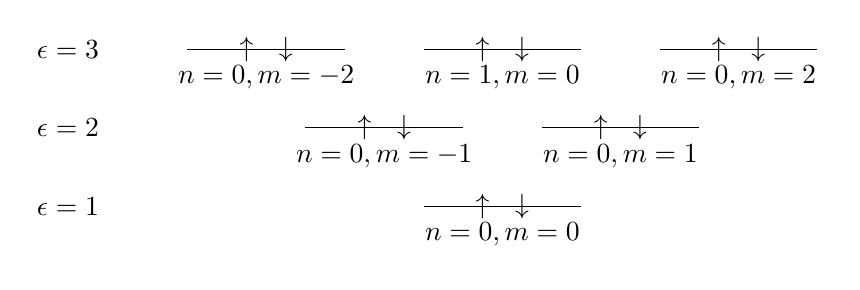
\begin{tikzpicture}
                        \begin{scope}
                            \foreach \i in {1, 2, 3} {
                                \draw(-1, \i - 1) node[anchor=east]
                                {$\epsilon = \i$};
                            }

                            % Highest energy level
                            \foreach \i in {0, 3, 6} {
                                \draw (\i, 2) -- (\i + 2, 2);
                                \node at (\i + 0.75, 2) {$\uparrow$};
                                \node at (\i + 1.25, 2) {$\downarrow$};
                            }
                            \node[below, inner sep=.2cm] at (1, 2)
                            {$n = 0, m = -2$};
                            \node[below, inner sep=.2cm] at (4, 2)
                            {$n = 1, m = 0$};
                            \node[below, inner sep=.2cm] at (7, 2)
                            {$n = 0, m = 2$};

                            % Middle energy level
                            \foreach \i in {1.5, 4.5} {
                                \draw (\i, 1) -- (\i + 2, 1);
                                \node at (\i + 0.75, 1) {$\uparrow$};
                                \node at (\i + 1.25, 1) {$\downarrow$};
                            }
                            \node[below, inner sep=.2cm] at (2.5, 1)
                            {$n = 0, m = -1$};
                            \node[below, inner sep=.2cm] at (5.5, 1)
                            {$n = 0, m = 1$};

                            % Lowest energy level
                            \draw (3, 0) -- (5, 0);
                            \node at (3 + 0.75, 0) {$\uparrow$};
                            \node at (3 + 1.25, 0) {$\downarrow$};
                            \node[below, inner sep=.2cm] at (4, 0)
                            {$n = 0, m = 0$};
                        \end{scope}
                    \end{tikzpicture}
                \end{center}
                \caption{In this plot we can see the energy degeneracy of the lowest
                three energy levels in the two-dimensional quantum dot.
                Each arrow representes a spin up or a spin down state with the
                quantum numbers $n$ and $m$ as listed below.
                This pattern goes on indefinitly with the addition of one bar
                (two oscillators) per level.}
                \label{fig:tdho-energy-levels}
            \end{figure}


        \subsubsection{Mapping the quantum numbers to a single value}
            When working with second quantized operators, we distinguish single
            particle functions in a Slater determinant by a single index.
            Including spin in the two-dimensional harmonic oscillator
            eigenstates we have to deal with three quantum numbers $n$, $m$, and
            $m_s$ per state.
            We are thus interested in finding a mapping $(n, m) \mapsto p$ and
            the inverse mapping $p \mapsto (n, m)$.\footnote{%
                The spin quantum number is easiest to deal with in the end as we
                can double each dimension in every matrix and label all odd or
                even indices by a spin direction.
            }
            Due to the degeneracy of the eigenenergies such a mapping will not
            be unique.
            We thus have to decide in advance how we should count the basis
            states.
            In this thesis we choose the convention that we start from the
            lowest energy level and move up by counting from left to right.
            Tabulating \autoref{fig:tdho-energy-levels} we get the table shown
            in \autoref{tab:tdho-mapping}.
            In \autoref{alg:nm-to-p} we give a sketch of the algorithm we use to
            compute $(n, m) \mapsto p$. We show the inverse algorithm in
            \autoref{alg:p-to-nm}.

            Using the aforementioned mapping we can find indices $p$ such that
            \begin{align}
                \ket{\psi_{nm}} \mapsto \ket{\psi_p},
            \end{align}
            and similarly for the eigenenergies
            \begin{align}
                \epsilon_{nm} \mapsto \epsilon_{p}.
            \end{align}

            \begin{table}
                \centering
                \caption{In this table we show an example of how our mapping
                convention will index the states shown in
                \autoref{fig:tdho-energy-levels}.}
                \renewcommand{\arraystretch}{1.3}
                \begin{tabular}{@{}lll@{}}
                    \toprule
                    $\epsilon_{nm}$ & $(n, m)$ & $p$ \\
                    \midrule
                    $1$ & $(0, 0)$ & $0$ \\
                    $2$ & $(0, -1)$ & $1$ \\
                    $2$ & $(0, 1)$ & $2$ \\
                    $3$ & $(0, -2)$ & $3$ \\
                    $3$ & $(1, 0)$ & $4$ \\
                    $3$ & $(0, 2)$ & $5$ \\
                    \bottomrule
                \end{tabular}
                \label{tab:tdho-mapping}
            \end{table}

            \begin{algorithm}
                \inputpython{implementation/quantum-systems/get_index_p.py}{0}{35}
                \caption{In this algorithm we describe how we can find $(n, m)
                \mapsto p$ relatively quick without having to tabulate all
                maps.}
                \label{alg:nm-to-p}
            \end{algorithm}

            \begin{algorithm}
                \inputpython{implementation/quantum-systems/get_indices_nm.py}{0}{48}
                \caption{In this algorithm we sketch how we can find $p \mapsto
                (n, m)$, i.e., the inverse of \autoref{alg:nm-to-p}.}
                \label{alg:p-to-nm}
            \end{algorithm}

        \subsubsection{Computing the dipole moments}
            The matrix elements of the dipole moment of the two-dimensional
            harmonic oscillator quantum dot is given by
            \begin{align}
                \vf{d}_{ij}
                \equiv \mel{i}{\positionvec}{j},
            \end{align}
            where we get a dipole moment for each coordinate in $\vf{r}$. As
            we've expressed the single particle functions in polar coordinates,
            but wish to express the dipole moments in a cartesian coordinate
            system, we have to compute the two integrals
            \begin{align}
                \vf{d}_{ij}
                &= \vf{i}\mel{i}{\position}{j}
                + \vf{j}\mel{i}{\position[y]}{j}
                = \vf{i}\mel{i}{r \cos(\phi)}{j}
                + \vf{j}\mel{i}{r \sin(\phi)}{j},
                \label{eq:dipole_elements}
            \end{align}
            where $\vf{i}$ and $\vf{j}$ are the unit vectors along the $x$- and
            $y$-axis respectively.
            Using \autoref{eq:eigenstate-tdho} we are able to find analytical
            expressions for the angular integral.
            The radial integral must be evaluated from $0$ to $\infty$, but
            lucikly SymPy \cite{sympy} handles this for us.
            Note that we use the notation $i \mapsto (n_i, m_i)$ from the
            mapping algorithms described above. We then get the following
            integrals
            \begin{align}
                \mel{i}{r \cos(\phi)}{j}
                &= N^{*}_{n_i m_i} N_{n_j m_j}
                \mathcal{R}_{ij}
                \mathcal{C}_{ij},
                \\
                \mel{i}{r \sin(\phi)}{j}
                &= N^{*}_{n_i m_i} N_{n_j m_j}
                \mathcal{R}_{ij}
                \mathcal{S}_{ij},
            \end{align}
            where no summation is implied in the index labels.
            The integrals are given by
            \begin{gather}
                \mathcal{R}_{ij}
                =
                \int_{0}^{\infty} \dd r r^2
                R_{n_i m_i}^{*}(r) R_{n_j m_j}(r),
                \label{eq:radial-integral-tdho}
                \\
                \mathcal{C}_{ij}
                =
                \int_{0}^{2\pi}
                \dd \phi
                \cos(\phi)
                \Phi_{m_i}^{*}(\phi)
                \Phi_{m_j}(\phi),
                \label{eq:cos-integral-tdho}
                \\
                \mathcal{S}_{ij}
                =
                \int_{0}^{2\pi}
                \dd \phi
                \sin(\phi)
                \Phi_{m_i}^{*}(\phi)
                \Phi_{m_j}(\phi).
                \label{eq:sin-integral-tdho}
            \end{gather}
            We solve the radial integral using SymPy \cite{sympy}.
            We start by constructing the radial functions $R_{n_i m_i}(r)$.
            This is done by the Python function shown in
            \autoref{alg:radial-function-tdho}, where the mapping from $i
            \mapsto (n_i, m_i)$ is done by \autoref{alg:p-to-nm}.
            \begin{algorithm}
                \inputpython{implementation/quantum-systems/spf_radial_function.py}{0}{10}
                \caption{Python function constructing the radial functions from
                the \autoref{eq:radial-function-tdho}.}
                \label{alg:radial-function-tdho}
            \end{algorithm}
            Having constructed the two radial functions we can perform the
            integraion using the function in \autoref{alg:radial-integral-tdho}.
            \begin{algorithm}
                \inputpython{implementation/quantum-systems/radial_integral.py}{0}{7}
                \caption{Python function performing the radial integral in
                \autoref{eq:radial-integral-tdho} using SymPy \cite{sympy} to
                evaluate the integral from $r \in [0, \infty)$.}
                \label{alg:radial-integral-tdho}
            \end{algorithm}

            The two angular integrals in \autoref{eq:cos-integral-tdho} and
            \autoref{eq:sin-integral-tdho} have closed form solutions which we
            derive.
            Starting with \autoref{eq:cos-integral-tdho} we can write
            \begin{align}
                \mathcal{C}_{ij}
                &=
                \int_{0}^{2\pi}
                \dd \phi
                \cos(\phi)
                \exp[-i\Delta m_{ij} \phi],
            \end{align}
            where we've defined the difference in the angular quantum number by
            \begin{align}
                \Delta m_{ij} \equiv m_i - m_j.
                \label{eq:diff-m-tdqd}
            \end{align}
            and we have that $\Delta m_{ij} \in \mathbb{Z}$.
            The closed form solution to this integral is
            \begin{align}
                \mathcal{C}_{ij}
                &= \brak{
                    \frac{\exp[-i\Delta m_{ij} \phi]}{1 - (\Delta m_{ij})^2}
                    \brak{
                        -i\Delta m_{ij} \cos(\phi)
                        + \sin(\phi)
                    }
                }_{0}^{2\pi}
                = 0,
                \label{eq:dipole-x-tdqd}
            \end{align}
            if $\Delta m_{ij} \neq \pm 1$.
            For the case when $\Delta m_{ij} = \pm 1$ we solve the easier
            integral
            \begin{align}
                \mathcal{C}_{ij}
                &=
                \int_{0}^{2\pi}
                \dd \phi
                \cos(\phi) \exp[\mp i\phi]
                \\
                &=
                \int_{0}^{2\pi}
                \dd \phi
                \para{
                    \cos^2(\phi)
                    \mp i\cos(\phi)\sin(\phi)
                }
                = \pi.
            \end{align}
            % TODO: Discuss the connection to the allowed dipole transitions in
            % a harmonic oscillator.
            For the sine integral in \autoref{eq:sin-integral-tdho} we have
            \begin{align}
                \mathcal{S}_{ij}
                &=
                \int_{0}^{2\pi}
                \dd\phi
                \sin(\phi)
                \exp[-i\Delta m_{ij} \phi].
            \end{align}
            The closed form solution of this integral is similar to the form for
            the cosine-integral.
            Again we look at the situation when $\Delta m_{ij} \neq \pm 1$
            initially.
            \begin{align}
                \mathcal{S}_{ij}
                &= \brak{
                    \frac{\exp[-i\Delta m_{ij} \phi]}{1 - (\Delta m_{ij})^2}
                    \brak{
                        -i\Delta m_{ij} \sin(\phi)
                        + \cos(\phi)
                    }
                }_{0}^{2\pi}
                = 0.
                \label{eq:dipole-y-tdqd}
            \end{align}
            For $\Delta m_{ij} = \pm 1$ we get
            \begin{align}
                \mathcal{S}_{ij}
                &=
                \int_{0}^{2\pi}
                \dd\phi
                \sin(\phi)
                \exp[\mp i\phi]
                \\
                &=
                \int_{0}^{2\pi}
                \dd\phi
                \para{
                    \sin(\phi)\cos(\phi)
                    \mp i\sin^2(\phi)
                }
                = \mp i\pi.
            \end{align}
            The results for the angular integrals yields the selection rules for
            the dipole approximation for the two-dimensional harmonic
            oscillator.
            Unless $\Delta m_{ij} = \pm 1$, the transition between the states is
            not allowed in the dipole approximation, i.e., the integral
            vanishes.
            % TODO: Write the full expression for the dipole elements.
            % TODO: Add plot of the dipole moments.


        \subsubsection{Computing the Coulomb elements}
            Having found the basis functions and the elements of the one-body
            hamiltonian, we are left with the task of finding the two-body
            elements from the Coulomb interaction.
            Luckily, there exists an analytic formula finding these elements for
            the two-dimensional harmonic oscillator in polar coordinates.
            This formula is shown in appendix A in the article
            \citetitle{anisimovas1998energy} by
            \citeauthor{anisimovas1998energy} \cite{anisimovas1998energy}.
            Note that \citeauthor{anisimovas1998energy} interchanges the indices
            in the ket-part of their two-body integrals as opposed to our
            convention. That is, in our notation we would write
            \begin{align}
                \mel{ij}{\twohamil}{kl}
                &=
                \int\dd x_1\dd x_2
                \psi_{i}^{*}(x_1) \psi_{j}^{*}(x_2)
                \twoten
                \psi_{k}(x_1)\psi_{l}(x_2)
                \equiv
                \mel{ij}{\twohamil}{lk}_{AM},
            \end{align}
            where $ \bra{ij}\twohamil\ket{lk}_{AM}$ is the convention used by
            \citeauthor{anisimovas1998energy}.
            There are two significant symmetries included in the calculation of
            the two-body elements.
            The first occurs as the Hamiltonian is spin-independent and the
            second comes from the azimuthal quantum number $m$.
            This can be expressed as
            \begin{align}
                \mel{ij}{\twohamil}{kl}
                = \delta_{\sigma_i \sigma_k} \delta_{\sigma_j \sigma_l}
                \int\dd \vf{r}_1\dd \vf{r}_2
                \psi_{i}^{*}(\vf{r}_i) \psi_{j}^{*}(\vf{r}_2)
                \twoten
                \psi_{k}(\vf{r}_1)\psi_{l}(\vf{r}_2),
            \end{align}
            where the symmetry that $m_i + m_j = m_k + m_l$ is baked into the
            integral.
            The formula for computing the integral
            \begin{align}
                \mathcal{I}^{ij}_{kl}
                =
                \int\dd \vf{r}_1\dd \vf{r}_2
                \psi_{i}^{*}(\vf{r}_1) \psi_{j}^{*}(\vf{r}_2)
                \twoten
                \psi_{k}(\vf{r}_1)\psi_{l}(\vf{r}_2),
            \end{align}
            is rather involved and we've pushed it to
            \autoref{app:coulomb-elements}.


    \subsection{Two-dimensional double well quantum dot}
        Another interesting system to explore is the double well quantum dot,
        i.e., a quantum dot with a finite barrier in the potential trap.
        Building the barrier on top of the two-dimensional harmonic oscillator
        lets us reuse much of the machinery from the previous section.
        There are a multitude of ways to create a confining double well
        potential.
        In the following we'll be focusing on a double well with a sharp
        boundary for the barrier in either $x$- or $y$-direction.
        The one-body Hamiltonian of the double well with the barrier in the
        $x$-direction is given by
        \begin{align}
            \onehamil
            &=
            \frac{\momentum^2}{2m}
            + \half m \omega^2 \position[r]^2
            + \half m \omega^2 \para{
                \frac{1}{4} l^2 - l\abs{\position}
            }.
            \label{eq:one-body-2ddw}
        \end{align}
        % TODO: Give motivation for the shape of the double-well.
        % Discuss the constant term.
        In \autoref{eq:one-body-2ddw} we recognize the two first terms as the
        kinetic energy and the harmonic oscillator confining potential.
        Instead of finding an analytical expression for the full one-body
        Hamiltonian, as we did for the harmonic oscillator, we'll instead use
        the single-particle functions in \autoref{eq:eigenstate-tdho} as trial
        wave functions and use the variational method to find as good an
        estimate as possible to the underlying exact eigenpair.
        The one-body matrix elements can then be found from
        \begin{align}
            \oneten^{p}_{q}
            &= \epsilon_{p}\delta^{p}_{q}
            + \half m \omega^2\mel{p}{\para{
                \frac{1}{4} l^2 - l \abs{\position}
            }}{q}
            \\
            &= \epsilon_{p}\delta^{p}_{q}
            + \frac{1}{8} m \omega^2 l^2 \delta^{p}_{q}
            - \half m \omega^2 l \mel{p}{\abs{\position}}{q},
        \end{align}
        where we have used the mapping $(n, m) \to p$ from
        \autoref{alg:nm-to-p} described above and where
        the eigenenergies $\epsilon_p$ are given by
        \autoref{eq:eigenenergy-tdho}.
        The two first terms give a shifted harmonic oscillator potential, viz.
        \begin{align}
            \epsilon_p' = \epsilon_p + \frac{1}{8} m \omega^2 l^2.
        \end{align}
        The last term is the double well barrier and resembles the dipole matrix
        elements from \autoref{eq:dipole_elements} except for the absolute
        value.
        We rewrite the potential barrier in polar coordinates by
        \begin{gather}
            \abs{x} = r\abs{\cos(\phi)}, \\
            \abs{y} = r\abs{\sin(\phi)},
        \end{gather}
        where we've included the barrier in $y$-direction for the sake of
        generality.
        We can thus compute the barrier integrals using the eigenstates from the
        harmonic oscillator.
        \begin{gather}
            \mel{p}{\abs{\position}}{q}
            =
            N^{*}_{n_p m_p} N_{n_q m_q}
            \mathcal{R}_{pq} \tilde{\mathcal{C}}_{pq},
            \\
            \mel{p}{\abs{\position[y]}}{q}
            =
            N^{*}_{n_p m_p} N_{n_q m_q}
            \mathcal{R}_{pq} \tilde{\mathcal{S}}_{pq},
        \end{gather}
        where the normalization and the radial integral is the same as for the
        dipole moment in the harmonic oscillator system.
        Note again that no summation is implied in the indices for the
        integrals.
        The only difference is the absolute value on the periodic functions in
        the polar integrals.
        These integrals are given by
        \begin{gather}
            \tilde{\mathcal{C}}_{pq}
            =
            \int_{0}^{2\pi} \dd \phi
            \abs{\cos(\phi)}
            \Phi^{*}_{m_p}(\phi)
            \Phi_{m_q}(\phi),
            \\
            \tilde{\mathcal{S}}_{pq}
            =
            \int_{0}^{2\pi} \dd \phi
            \abs{\sin(\phi)}
            \Phi^{*}_{m_p}(\phi)
            \Phi_{m_q}(\phi).
        \end{gather}
        For $k \in \mathbb{Z}$ and $\Delta m_{pq} \equiv m_p - m_q$, the
        solution to the cosine integral is given by
        \begin{align}
            \tilde{\mathcal{C}}_{pq}
            =
            \frac{4}{1 - (\Delta m_{pq})^2}
            \begin{cases}
                0 & \Delta m_{pq} = 2k + 1, \\
                1 & \Delta m_{pq} = 4k, \\
                -1 & \Delta m_{pq} = 4k + 2,
            \end{cases}
        \end{align}
        and for the sine integral we get
        \begin{align}
            \tilde{\mathcal{S}}_{pq}
            &=
            \frac{4}{1 - (\Delta m_{pq})^2}
            \begin{cases}
                0 & \Delta m_{pq} = 2k + 1, \\
                1 & \Delta m_{pq} = 2k.
            \end{cases}
        \end{align}
        For a full derivation, see \autoref{app:barrier-integrals}.

        Having constructed the full one-body Hamiltonian matrix $\onemat$, we
        diagonalize and find the variationally optimized eigenvectors $\vf{C}$.
        We can now use the coefficients to transform to the new double-well
        basis.
        That is, we construct the single-particle functions
        \begin{align}
            \ket{\psi_{\alpha}} = C^{p}_{\alpha}\ket{\phi_p},
        \end{align}
        where we label the double-well single-particle functions by
        $\ket{\psi_{\alpha}}$ with greek indices to distinguish from the known
        harmonic oscillator single-particle functions $\ket{\phi_p}$.
        Stated as an eigenequation for the double-well one-body Hamiltonian
        \begin{gather}
            \onehamil \ket{\psi_{\alpha}}
            = \varepsilon_{\alpha} \ket{\psi_{\alpha}}
            \implies
            \onehamil C^{q}_{\alpha} \ket{\phi_q}
            = \varepsilon_{\alpha} C^{q}_{\alpha} \ket{\phi_q},
        \end{gather}
        where we've inserted the known single-particle functions along with the
        coefficients.
        The eigenenergy $\varepsilon_{\alpha}$ is the eigenenergy of the
        double-well single-particle functions.
        Projecting onto the harmonic oscillator basis, we find a generalized
        eigenvalue equation.
        \begin{gather}
            \bra{\phi_{p}}\onehamil\ket{\phi_q} C^{q}_{\alpha}
            = \varepsilon_{\alpha} C^{q}_{\alpha} \braket{\phi_{p}}{\phi_{q}}.
        \end{gather}
        Recalling that the harmonic oscillator basis is orthonormal and
        inserting the matrix elements for the one-body Hamiltonian we are left
        with
        \begin{align}
            \oneten^{p}_{q} C^{q}_{\alpha}
            = \delta^{p}_{q} C^{q}_{\alpha} \varepsilon_{\alpha}
            = C^{p}_{\alpha} \varepsilon_{\alpha}.
        \end{align}
        Solving this generalized eigenvalue equation yields the coefficient
        matrix, $\vf{C} \in \mathbb{C}^{L\times L}$, and the eigenenergy matrix
        $\vfg{\varepsilon} = \diag(\varepsilon_1, \dots, \varepsilon_L)$, where
        $L$ is the number of harmonic oscillator basis functions.
        Having found the coefficient matrix we can transform the two-body
        elements from the harmonic oscillator basis to the double-well basis by
        \begin{align}
            \bra{\psi_{\alpha} \psi_{\beta}}
            \twohamil
            \ket{\psi_{\gamma} \psi_{\delta}}
            = {C^{p}_{\alpha}}^{*}
            {C^{q}_{\beta}}^{*}
            \bra{\phi_{p} \phi_{q}}
            \twohamil
            \ket{\phi_{r} \phi_{s}}
            C^{r}_{\gamma}
            C^{s}_{\delta}.
        \end{align}
        The same procedure can also be used on other matrix elements defined in
        the harmonic oscillator basis. For example, the dipole matrix elements
        yields
        \begin{align}
            \bra{\psi_{\alpha}}
            \vf{d}
            \ket{\psi_{\beta}}
            = {C^{p}_{\alpha}}^{*}
            \bra{\phi_{p}}
            \vf{d}
            \ket{\phi_{q}}
            C^{q}_{\beta}.
        \end{align}

        \subsubsection{Quality of the transformed single-particle functions}
            As the harmonic oscillator basis in no way is a complete basis
            covering enough of the Hilbert space in order to accurately describe
            the double-well basis, we need to make a choice on how many basis
            functions we deem ``good enough''.
            % TODO: This sentence needs rephrasing.


    \section{Atomic and molecular systems}
        \label{sec:atoms-and-molecules}
        Having discussed systems of quantum dots, or so-called ``artificial
        atoms'', we will now focus on actual atomic and molecular systems.
        As stated at the start of this chapter we make use of existing
        libraries to construct atomic and molecular basis sets.
        We will therefore touch briefly on the topic of atomic and molecular
        basis sets as much of the work therein will be treated as a black box.
        The molecular electronic one-body Hamiltonian in the Born-Oppenheimer
        approximation is given by \cite{basis-sets, hochstuhl2014time}
        \begin{align}
            \onehamil_i
            = -\half \nabla^2_i
            - \frac{Z_A}{\abs{\vfg{R}_A - \vfg{r}_i}},
        \end{align}
        where atomic units are assumed.
        Note that we sum over all nuclei $A$.
        Here we've left out the internuclear repulsion and the Coulomb
        interaction.
        Furthermore, in the Born-Oppenheimer approximation we treat the nuclei
        as being frozen and therefore ignore the kinetic energy contribution of
        the nuclear core.

        Now, perhaps not surprisingly the exact solution of the full molecular
        Hamiltonian\footnote{%
            Even in the Born-Oppenheimer approximation.
        } is a far fetched goal for all but the smallest systems to say the
        least.
        Similar to the procedure we did for the double-well in
        \autoref{subsec:tddw} we can solve the molecular Hamiltonian in an
        approximate basis set.
        We can then diagonalize the one-body Hamiltonian and express the
        matrix elements in this new basis.
        As a consequence a lot of effort in the quantum chemistry field has been
        put into the construction of efficient and good basis sets.
        We will in this thesis use the following basis sets:
        \begin{itemize}
            \item The minimal Slater-type orbital (STO-$k$G) basis sets
                \cite{sto-3g}.
                Here $k$ denotes the number of Gaussian primitive functions used
                in a single basis function.
            \item The split-valence ($X$-$YZ$g) basis sets \cite{x-yzg}.
                Here $X$ denotes the number of primitive Gaussian functions for
                the core basis functions.
                The $Y$ and $Z$ tells us that there are two sets of basis
                functions with $Y$ and $Z$ basis functions for the valence
                orbitals respectively.
            \item The correlation-consistent polarized valence (cc-pV$X$Z) basis
                sets \cite{cc-pVXZ}.
                These basis sets are better tuned for post Hartree-Fock methods.
                The $X$ parameter decides the number of functions for the
                valence electrons, e.g., $D$ for double-zeta, $T$ for
                triple-zeta, etc.
            \item The augmented correlation-consistent (aug-cc-pV$X$Z) basis
                sets \cite{aug-cc-pVXZ}.
                The cc-pV$X$Z basis sets are designed for ground state
                calculations, but are inferior when it comes to describing
                excited states.
                The aug-cc-pV$X$Z basis functions alleviates some of this by
                incuding diffuse functions for the outer valence electrons
                \cite{helgaker-molecular}.
                The parameter $X$ is the same as in the case of the cc-pV$X$Z
                basis set.
        \end{itemize}
        To reuse the basis sets from PySCF \cite{pyscf} and Psi4 \cite{psi4}
        we've created a class \pyth{CustomSystem} which lets us build a
        \pyth{QuantumSystem}-class by manually setting the matrix elements.
        We can thus ask PySCF and Psi4 to use their well-optimized methods to
        generate basis sets and reuse these in our solvers.
        In this thesis we will only use basis sets from PySCF and we therefore
        only describe the interface towards this library.

        We've created three interface functions which sets up a
        \pyth{CustomSystem} of atomic orbitals, restricted molecular orbitals,
        and unrestricted molecular orbitals respectively.
        The two latter methods use the restricted and unrestricted Hartree-Fock
        solvers of PySCF.
        There are two main input parameters to these functions and that is
        \pyth{molecule} and \pyth{basis}.
        The former is a string describing the atom or molecule.
        In case of an atom it is enough to write the chemical symbol for the
        atom, e.g., \pyth{"he"} for Helium.
        For molecules the coordinates of the atoms contained in the system must
        be included.
        In the case of diatomic molecules we can then specify a bond distance
        along a specific axis, e.g., \pyth{f"h 0 0 0; h 0 0 1.2"} for the
        \ch{H2}-molecule with the bond distance $1.2$ specified in atomic units
        along the $z$-axis.
        The basis strings share the same format as discussed above, e.g., to
        specify the usage of aug-cc-pVDZ, we pass in the string
        \pyth{"aug-ccpvdz"} as the basis.


    \section{Particle density}
        \label{sec:particle-density}
        From \autoref{subsec:particle-density} we know how to compute the
        one-body particle density once we have found the one-body density matrix
        from a specific solver.
        For variational methods where the dual state of $\ket*{\phi_p}$ is the
        adjoint $\bra*{\phi_p}$ we can use the expression in
        \autoref{eq:particle-density}.
        However, as we are focusing much of our work on the bi-variational
        formulation of coupled-cluster we will implement the more general
        particle-density calculation
        \begin{align}
            \densityten(x)
            = \tilde{\phi}_{q}(x)
            \densityten^{q}_{p}
            \phi_p(x),
        \end{align}
        where $\tilde{\phi}_q(x)$ is the bi-variational dual state of
        $\phi_p(x)$.
        For the Hartree-Fock methods and configuration-interaction solvers we
        choose $\tilde{\phi}_q(x) = \phi^{*}_q(x)$ and we have recovered the
        original expression for the particle density as seen in
        \autoref{eq:particle-density}.
        In \autoref{alg:particle-density} we've included the code used to
        compute the particle density given a one-body density matrix denoted
        \pyth{rho_qp}, and the set of orbitals \pyth{bra_spf} and \pyth{ket_spf}
        as the bra- and ket-states respectively.
        We let the first index (the rows) of the orbital arrays denote the
        orbital index $p$, $q$, etc, whereas the remaining indices define the
        evaluation of the function on a $d$-dimensional grid $x \in
        \mathbb{C}^{d}$.
        \begin{algorithm}
            \begin{python}
def compute_particle_density(rho_qp, bra_spf, ket_spf):
    rho = np.zeros(ket_spf.shape[1:], dtype=ket_spf.dtype)
    spf_slice = slice(0, ket_spf.shape[0])

    for _i in np.ndindex(rho.shape):
        i = (spf_slice, *_i)
        rho[_i] += np.dot(bra_spf[i], np.dot(rho_qp, ket_spf[i]))

    return rho
            \end{python}
            \caption{In this listing we've added a function computing the
            particle density on an arbitrary grid that the orbitals are
            evaluated on.}
            \label{alg:particle-density}
        \end{algorithm}

    \section{Change of basis}
        \label{sec:change-of-basis}
        Much of what we do in this thesis is related to basis transformations.
        Either by diagonalization of the one-body Hamiltonian, an initial
        Hartree-Fock calculation, or in the orbital rotations in the
        non-orthogonal and orbital-adaptive coupled-cluster methods.
        A basis transformation can in general be represented by
        \begin{align}
            \ket*{\psi_p} = C_{\alpha p} \ket*{\phi_{\alpha}},
            \label{eq:spf-basis-change}
        \end{align}
        where we use greek indices to denote a basis of $K$ orbitals
        $\brac{\phi_{\alpha}}$ and latin letters for the basis of $L$
        transformed orbitals $\brac{\psi_p}$, and where $\vfg{C} \in
        \mathbb{C}^{K\times L}$ is a complex matrix with the coefficients
        necessary for the transformation.

        Having found the coefficient matrix $\vfg{C}$ we can change basis for
        all the existing matrix elements stored in the
        \pyth{QuantumSystem}-class.
        We will also here assume for the sake of generality that the dual states
        $\tilde{\psi}_p$ and $\tilde{\phi}_{\alpha}$ are not necessarily the
        adjoints of $\psi_p$ and $\phi_{\alpha}$.
        This means that
        \begin{align}
            \bra*{\tilde{\psi}_p}
            = \tilde{C}_{p \alpha}\bra*{\tilde{\phi}_{\alpha}}.
            \label{eq:spf-dual-basis-change}
        \end{align}
        Take extra note of the ordering of the indices in the coefficients in
        the dual basis transformation.
        In the case of adjoint states we have the familiar $\tilde{C}_{p \alpha}
        = C^{*}_{\alpha p}$.
        From the list of contents in \pyth{QuantumSystem} at the top of this
        chapter, we have three types of basis transformations that we need to
        support to fully change our system.
        We need to be able to change basis for one- and two-body matrix
        elements, and for the single-particle functions.

        We denote arbitrary one-body matrix elements of the one-body matrix
        $\vfg{\oneten}$ in the original orbital basis by
        \begin{align}
            \oneten_{\alpha \beta}
            \equiv
            \mel*{\tilde{\phi}_{\alpha}}{\onehamil}{\phi_{\beta}}.
        \end{align}
        Transforming to the new basis set we have
        \begin{gather}
            \tilde{\oneten}_{pq}
            = \mel*{\tilde{\psi}_p}{\onehamil}{\psi_q}
            =
            \tilde{C}_{p\alpha}
            \oneten_{\alpha \beta}
            C_{\beta q}
            \implies
            \tilde{\vfg{\oneten}}
            = \tilde{\vfg{C}}
            \vfg{\oneten}
            \vfg{C},
        \end{gather}
        where $\tilde{\vfg{\oneten}}$ is the transformed one-body elements.
        An implementation of the change of basis for the one-body elements is
        shown in \autoref{alg:transform-one-body-elements}.
        In the case of the dipole moments we store these as an array of one-body
        elements, one for every dimension, which means that we need to transform
        each axis using the algorithm in
        \autoref{alg:transform-one-body-elements}.
        \begin{algorithm}
            \begin{python}
def transform_one_body_elements(h, c, c_tilde=None):
    if c_tilde is None:
        c_tilde = c.conj().T

    return c_tilde @ h @ c
            \end{python}
            \caption{This function changes basis for the one-body matrix
            elements given a coefficient matrix \pyth{c} and an optional dual
            coefficient matrix \pyth{c_tilde}.}
            \label{alg:transform-one-body-elements}
        \end{algorithm}
        For the two-body elements we denote the elements by
        \begin{align}
            \twoten^{\alpha\beta}_{\gamma\delta}
            \equiv
            \mel*{\tilde{\phi}_{\alpha}\tilde{\phi}_{\beta}}{
                \twohamil
            }{\phi_{\gamma}\phi_{\delta}},
        \end{align}
        where we do not care if the elements are antisymmetric or not as it does
        not change the basis transformation.
        The transformation can now be done by
        \begin{align}
            \tilde{\twoten}^{pq}_{rs}
            = \mel*{\psi_p\psi_q}{
                \twohamil
            }{\psi_r\psi_s}
            = \tilde{C}_{p\alpha}
            \tilde{C}_{q\beta}
            \twoten^{\alpha\beta}_{\gamma\delta}
            C_{\gamma r}
            C_{\delta s}.
        \end{align}
        In \autoref{alg:transform-two-body-elements} we demonstrate the function
        which changes the basis for the two-body elements.
        We make use of temporary storage of a two-body matrix \pyth{_u} which
        lowers the cost of the basis transformation from $\mathcal{O}(L^8)$ to
        $\mathcal{O}(L^5)$.
        \begin{algorithm}
            \begin{python}
def transform_two_body_elements(u, c, c_tilde=None):
    if c_tilde is None:
        c_tilde = c.conj().T

    # abcd, ds -> abcs
    _u = np.tensordot(u, c, axes=(3, 0))
    # abcs, cr -> absr -> abrs
    _u = np.tensordot(_u, c, axes=(2, 0)).transpose(0, 1, 3, 2)
    # abrs, qb -> arsq -> aqrs
    _u = np.tensordot(_u, c_tilde, axes=(1, 1)).transpose(
        0, 3, 1, 2
    )
    # pa, aqrs -> pqrs
    _u = np.tensordot(c_tilde, _u, axes=(1, 0))

    return _u
            \end{python}
            \caption{This function changes the basis of the two-body elements
            given a coefficient matrix \pyth{c} and an optional dual matrix
            \pyth{c_tilde}.}
            \label{alg:transform-two-body-elements}
        \end{algorithm}
        For the single-particle functions the basis transformation is performed
        by \autoref{eq:spf-basis-change} and \autoref{eq:spf-dual-basis-change}
        where the states are projected on a grid.
        We represent all the single-particle states as a $d + 1$-dimensional
        array, where the first axis denotes which single-particle state we are
        looking at, and the $d$-remaining axes denotes the grid.
        In \autoref{alg:transform-spfs} we show the member function of
        \pyth{QuantumSystem} for changing the single-particle state basis.
        \begin{algorithm}
            \begin{python}
class QuantumSystem:
    # Code removed for clarity

    def change_basis_spf(self, c, c_tilde=None):
        if c_tilde is not None:
            # In case of bi-orthogonal basis sets, we create an
            # extra set of single-particle functions for
            # the bra-side
            self._bra_spf = self.np.tensordot(
                c_tilde,
                self._spf.conj()
                if self._bra_spf is None else self._bra_spf,
                axes=((1), (0)),
            )

        self._spf = self.np.tensordot(
            c, self._spf, axes=((0), (0))
        )
            \end{python}
            \caption{Here we list the member function in \pyth{QuantumSystem}
            that transforms the single-particle states given a coefficient
            matrix \pyth{c} and an optional dual matrix \pyth{c_tilde}.
            The single-particle states are denoted \pyth{self._spf} and
            \pyth{self._bra_spf} in case of a dual state that is not the adjoint
            state.}
            \label{alg:transform-spfs}
        \end{algorithm}


    \section{Spin-doubling}
        The basis sets we are exploring are always formulated as spatial
        orbitals without any spin component.
        Furthermore, we look at spin-independent Hamiltonians for the most
        part\footnote{%
            We explore a spin-dependent laser field to some extent as will be
            demonstrated in the results.
        } and a restricted solution can be used where we incorporate the spin by
        reusing the doubly occupied orbitals.
        We will use this to some extent for the restricted Hartree-Fock solver
        which will be discussed in \autoref{subsec:rhf}.
        However, most of the methods we've implemented make no assumption on the
        spin-orbitals other than there being two spin-components, and therefore
        allow general spin-orbitals as discussed in
        \autoref{subsec:restrictions-on-spin-orbitals}.
        This means that after we've created our basis sets, we include spin by
        making the system doubly degenerate in each orbital.

        The ordering of the spin-orbitals are important as some solvers
        exploit the spin-degeneracy and therefore need to know how the
        spin-orbitals are ordered.
        We've chosen a solution which is far from optimal, but which is
        reasonable as long as we have an even number of particles with the same
        amount of particles in each spin-direction.
        We use the convention that orbitals are ordered in an increasing order
        based on their single-particle eigenenergy.\footnote{%
            This is the ordering that is returned by NumPy when diagonalizing
            the one-body Hamiltonian.
        }
        We then double the length of each orbital axis in the single-particle
        functions,\footnote{%
            Except for the grid axes.
        } the one-body- and two-body Hamiltonians, and all other matrix
        elements.
        Next we repeat each orbital twice so that even indices correspond to a
        certain spin-direction and odd indices to the other direction.
        We are able to achieve this quite succintly using the Kronecker-product
        and slicing in NumPy.
        In \autoref{alg:spin-doubling-spf} we demonstrate a snippet which adds
        spin to a set of orbitals defined on an arbitrary grid.
        \begin{algorithm}
            \begin{python}
class QuantumSystem:
    # Code removed for clarity

    def change_to_spin_orbital_basis(self, anti_symmetrize=True):
        # Code removed for clarity

        if not self._spf is None:
            new_shape = [
                self._spf.shape[0] * 2, *self._spf.shape[1:]
            ]

            spf = self.np.zeros(
                tuple(new_shape), dtype=self._spf.dtype
            )
            spf[::2] += self._spf
            spf[1::2] += self._spf

            self._spf = spf
            assert self._spf.shape[0] == self.l
            \end{python}
            \caption{Spin-doubling of the single-particle functions.}
            \label{alg:spin-doubling-spf}
        \end{algorithm}
        For the one-body elements we use the function listed in
        \autoref{alg:spin-doubling-one-body}.
        The two-body elements requires us to do some more work as the Kronecker
        product gets applied to the two last indices of the array.
        We also want the product to be applied to pairwise indices that interact
        in the two-body integrals.
        This requires some transposing of the elements, and is shown in
        \autoref{alg:spin-doubling-two-body}.
        \begin{algorithm}
            \begin{python}
def add_spin_one_body(h):
    return np.kron(h, np.eye(2))
            \end{python}
            \caption{Function adding spin to one-body matrix elements, that is,
            matrices.}
            \label{alg:spin-doubling-one-body}
        \end{algorithm}
        \begin{algorithm}
            \begin{python}
def add_spin_two_body(_u):
    u = _u.transpose(1, 3, 0, 2)
    u = np.kron(u, np.eye(2))
    u = u.transpose(2, 3, 0, 1)
    u = np.kron(u, np.eye(2))
    u = u.transpose(0, 2, 1, 3)

    return u
            \end{python}
            \caption{Function adding spin to the two-body elements.}
            \label{alg:spin-doubling-two-body}
        \end{algorithm}

        A more general solution -- and which should be implemented in the future
        -- is to create spin-blocks with each spin-direction following each
        other as this allows for an unequal number of particles in each
        spin-direction.
        This is the solution that needs to be taken for the unrestricted
        Hartree-Fock method when changing basis.

    \section{Time-evolution operators}
        The only time-evolution operators used in this thesis are dipole lasers
        in the length gauge.
        We've implemented this by allowing \pyth{QuantumSystem} to have a
        pointer to a \pyth{TimeEvolutionOperator}-class, where \pyth{LaserField}
        is a subclass.
        The \pyth{LaserField}-class takes in the parameter \pyth{laser_pulse}
        and an optional \pyth{polarization_vector}.
        The former parameter is the electric field of the laser including the
        envelope function, whereas the latter defines which axis to polarize
        along.
        By default the polarization vector is set along the $x$-axis, that is,
        the first axis.
        Note that \pyth{QuantumSystem} so far does not have a charge which means
        that for negative charge either the pulse or the polarization vector
        needs to incorporate this sign.
        Both \pyth{laser_pulse} and \pyth{polarization_vector} can be constants
        or functions of a single parameter; time.
        We restrict our attention to a constant linear polarization, but we use
        time-dependent laser pulses.
        To specify a laser pulse, the user creates a function or a class with a
        \pyth{__call__}-method which takes in a single parameter as time.
        This function should return the electric field at the given time
        including the envelope function.

    \section{Measuring the dipole moment}
        In order to measure the dipole moment in time we use the one-body
        density matrix from the given solver to compute
        \begin{align}
            \expval*{\vfg{d}(t)}
            = \densityten^{q}_{p}(t)\vfg{d}^{p}_{q},
        \end{align}
        where the time-dependence is kept in the one-body density matrix.
        For the time-dependent Hartree-Fock method and the orbital-adaptive
        time-dependent coupled-cluster methods we have to make sure that we
        change basis at each time step before computing the trace of the
        one-body density matrix and the dipole moment.
        This yields a time-dependent dipole moment.
        Note also that we choose a specific axis of the dipole moment.


        % Theory on computational aspects of the methods
        \chapter{Computational aspects}
    Along with this thesis we have implemented several quantum-mechanical
    solvers that are separated into different Github repositiories.\footnote{%
        Due to ongoing publications using the code most of the repositiories are
        at the time of writing private and access are therefore limited to
        collaborators.
        However, please do request access by sending a mail to:
        \href{mailto:o.s.schoyen@fys.uio.no}{o.s.schoyen@fys.uio.no}, and we'll
        set you up.
    }
    \begin{itemize}
        \item Quantum-systems is a Python package containing modules to set up
            matrix elements, time-evolution operators, and single-particle
            states to be used by the many-body solvers.
            Quantum-systems provides interfaces to the PySCF \cite{pyscf} and
            Psi4 \cite{psi4} systems.
            The code is located at
            \url{https://github.com/Schoyen/quantum-systems} with the
            documentation at
            \url{https://schoyen.github.io/quantum-systems/}.
        \item Coupled-cluster is a Python package with modules containing ground
            state and time-dependent coupled cluster solvers.
            Currently this packages contains doubles, singles-and-doubles ,
            non-orthogonal coupled cluster doubles, and the orbital adaptive
            time-dependent coupled cluster doubles methods.
            The module uses quantum-systems to get access to matrix elements.
            The code is located at
            \url{https://github.com/Schoyen/coupled-cluster} with the
            documentation at
            \url{https://schoyen.github.io/coupled-cluster/}.
        \item Configuration-interaction is a package containing ground state and
            time-dependent configuration interaction solvers.
            This code supports arbitrary levels of excitations, e.g.,
            singles-and-doubles, doubles-and-triples, etc, and full
            configuration interaction.
            The module uses quantum-systems to get access to matrix elements.
            The code is located at
            \url{https://github.com/Schoyen/configuration-interaction} with
            the documentation at
            \url{https://schoyen.github.io/configuration-interaction/}.
        \item Hartree-Fock is a package containing ground state and
            time-dependent Hartree-Fock solvers.
            We've implemented Hartree-Fock for general, restricted and
            unrestricted spin-orbitals.
            The module uses quantum-systems to get access to matrix elements.
            The code is located at
            \url{https://github.com/Schoyen/hartree-fock} with
            the documentation at
            \url{https://schoyen.github.io/hartree-fock/}.
    \end{itemize}
    We will in the rest of this chapter discuss various aspects of the
    implementation that we deem important to elaborate on, but we will leave
    specific implementation details and usage of the solvers to the
    repositiories and the documentation.

    \section{Why Python?}
        In working with this thesis we have developed a large computational
        framework for performing real-time quantum mechanics simulations for
        many-body problems in the programming language Python \cite{python}.
        The choice of using Python comes with a list of pros and cons.
        \begin{itemize}
            \item The development time is much lower when using Python as
                opposed to more verbose, but efficient languages such as C/C++,
                and Fortran.
            \item Integration with other Python libraries are relatively easy.
            \item Libraries such as SciPy \cite{scipy}, NumPy \cite{numpy}, and
                SymPy \cite{sympy} provides fast, and efficient interfaces to
                BLAS and LAPACK along with convenient array abstractions.
        \end{itemize}

    \section{Computing tensor contractions}
        Quite a significant amount of computational resources will go into the
        evaluation of tensor contractions\footnote{%
            We tend to call the matrix elements for tensors, but they more
            resemble numerical $N$-dimensional arrays.%
            % TODO: Check this footnote.
        } and we will therefore spend some time discussing how these
        contractions are performed and how we can speed up the contractions.

        Consider the antisymmetric, two-body, Coulomb elements given by
        \begin{align}
            \twoten^{pq}_{rs}
            = \mel{\phi_p\phi_q}{\twohamil}{\phi_r\phi_s}_{AS},
        \end{align}
        which, along with the two-body density matrix, is the largest tensor in
        use.
        This tensor often represents the bottleneck both in terms of memory and
        contraction time.
        When we represent these tensors mathematically, the labelling of the
        indices are in some sense arbitrary and depends on the context that the
        tensors are used.
        On a computer we however need to decide on a specific way of storing
        memory, and often this choice is related to speed concerns where some
        storage schemes show vast improvements in terms of cache hits as opposed
        to other schemes.
        However, tensor contractions are notoriously difficult to handle in
        terms of memory as they often involve change of dimensionality,
        re-ordering of indices resulting in the need of reshapes, and summation
        along axes that are inefficiently laid out in memory.
        % TODO: Add demonstration of this from CCD

        For the sake of generality we therefore ignore much of these problems
        and have decided to use a fixed layout of the memory and absorb the cost
        of reshapes and memory allocations.
        In our programs we read the axis from top-left and moving right before
        starting on bottom-left and going right.
        That is, to access element $\twoten^{pq}_{rs}$ we use the ordering
        \pyth{u[p, q, r, s]} in NumPy-arrays \cite{numpy}.
        This ordering is used consistenly for all tensors in all solver
        implementations.
        Other orderings might be smarter due to efficient usage of cache hits,
        but this clutters much of the implementation and is therefore ignored.

        \subsection{Intermediates}
            It is common in the coupled cluster litterature to talk about
            \emph{intermediates} \cite{hjorth2017advanced, gauss1995coupled}, or
            intermediate computations, as a technique for speeding up tensor
            contractions involving three or more tensors.
            The basics of intermediate computations is to treat a tensor
            contraction as a binary operation and precomputing common factors,
            or one of the contractions.
            As an example, consider the D3c term, sans the permutation opeator,
            from the coupled cluster doubles amplitudes in
            \autoref{tab:ccd-tau-amplitude-terms},
            \begin{align}
                g^{ab}_{ij} = \clustamp^{ab}_{lj} \clustamp^{dc}_{ik}
                \twoten^{kl}_{cd}.
            \end{align}
            The naïve solution using explicit for-loops yields a
            $\mathcal{O}(M^4 N^4)$-complexity.
            By first creating the intermediate contraction
            \begin{align}
                W^{l}_{i} = \clustamp^{dc}_{ik} \twoten^{kl}_{cd},
            \end{align}
            and then computing the total result from
            \begin{align}
                g^{ab}_{ij} = \clustamp^{ab}_{lj} W^{l}_{i},
            \end{align}
            we've reduced the complexity to $\mathcal{O}(M^2 N^3)$.
            This incurs a memory penalty from the temporary storage of
            $W^{l}_{i}$, but the gain in reduction of the number of FLOPS far
            exceeds this cost.

            The choice of which terms to use when creating intermediates has
            been explored in some depth, especially in the case of the
            coupled-cluster singles-and-doubles as done by
            \citeauthor{gauss1995coupled} \cite{gauss1995coupled}.
            We will however not employ pre-defined intermediates, but rather use
            the binary operator \pyth{np.tensordot} \cite{numpy} to do
            contractions.
            This forces us to pre-compute terms with three or more tensors thus
            lowering the cost.
            However, some care must be taken as the optimal choice depends on
            which terms are to be contracted.
            By inspection we choose the contractions which will yield the lowest
            amount of computational complexity by counting the number of unique
            indices and the lowest amount of storage cost.


    \section{Convergence acceleration}
        \label{sec:convergence}
        When performing optimization techniques such as the quasi-Newton method
        for the coupled-cluster equations and the self-consistent field
        iterations in Hartree-Fock, we often find that the solutions can have
        trouble converging.
        To alleviate some of these convergence issues we introduce two
        techniques which often lets us converge faster, or in some cases,
        converge at all.

        \subsection{Alpha filter}
            \label{subsec:alpha-filter}
            A first order approximation stems from data estimation theory as an
            alternative to the more sophisticated Kalman filter.
            This is a technique which lets us combine a predicted value and a
            measured value.
            % TODO: Cite slides:
            % https://www.uio.no/studier/emner/matnat/fys/FYS3240/v19/lecturenotes/l12---data-fusion.pdf
            Given a measurement $\vfg{x}^{(i)}$ at a time $i$ we can create an
            updated estimate $\bar{\vfg{z}}^{(i)}$ from a predicted estimate
            $\vfg{z}^{(i)}$ by
            \begin{align}
                \bar{\vfg{z}}^{(i)} = (1 - \alpha) \vfg{z}^{(i)}
                + \alpha \vfg{x}^{(i)},
            \end{align}
            where $\alpha \in \brak{0, 1}$ is a gain parameter.
            We have in our implementations perhaps (mis)named this filter for
            alpha mixing, as we ``mix'' some of the predicted and measured
            values in a new estimate.
            Note that for $\alpha = 0$ we only keep the predicted value
            $\vfg{z}^{(i)}$ whereas for $\alpha = 1$ we keep the raw
            measurements $\vfg{x}^{(i)}$.
            In our code we have dubbed the measurement vector by
            \pyth{trial_vector} and the predicted estimate by
            \pyth{direction_vector}.

        \subsection{Direct inversion of the iterative subspace}
            \label{subsec:diis}
            A more sophisticated acceleration technique is DIIS (direction
            inversion of the iterative subspace) acceleration
            \cite{pulay1980393, helgaker-molecular}.
            In order to estimate a measured vector $\vfg{p}^{(i + 1)}$ at a
            certain step $i + 1$ we use the linear combination
            \begin{align}
                \bar{\vfg{p}}^{(i + 1)} = \sum_{k = 1}^{i} c_k \vfg{p}^{(i)},
                \label{eq:diis-estimate}
            \end{align}
            where $\bar{\vfg{p}}_i$ is the estimated value at step $i$, and
            $c_k$ is a set of unknown coefficients subject to the constraint
            that they should sum up to unity at every step $i$.
            In order to find the coefficients, we construct an error vector
            $\vfg{e}_i$ from $\vfg{p}_i$.
            This step is dependent on the solver we are looking at and will be
            postponed to the implementation chapters on Hartree-Fock and
            coupled-cluster.
            For now, consider the extrapolated error vector
            \begin{align}
                \bar{\vfg{e}}_i
                = \sum_{k = 1}^{i - 1} c_k \vfg{e}_k,
            \end{align}
            calculated from the measured error vectors.
            We now wish to minimize the error, and we do this using Lagrange's
            method of undetermined multipliers in order to include the
            constraint that the coefficients should sum up to unity, viz.
            \begin{align}
                L &=  \norm{\bar{\vfg{e}}_i}^2
                - 2\lambda\para{
                    \sum_{k = 1}^{i - 1} c_i
                    - 1
                }.
                \label{eq:diis-lagrangian}
            \end{align}
            The squared norm of the error vectors can be expressed by
            \begin{align}
                \norm{\bar{\vfg{e}}_i}^2
                = c_k B_{kl} c_l,
            \end{align}
            where we've defined the matrix elements
            \begin{align}
                B_{kl} \equiv \vfg{e}_k^T\vfg{e}_l.
            \end{align}
            Finding the stationary condition of the Lagrangian in
            \autoref{eq:diis-lagrangian} with respect to the coefficients $c_k$
            we get system of $i$ linear equations.
            This can expressed as matrices by
            \begin{align}
                \begin{pmatrix}
                    B_{11} & \dots & B_{1i} & -1 \\
                    \vdots & \ddots & \vdots & \vdots \\
                    B_{i1} & \dots & B_{ii} & -1 \\
                    -1 & \dots & -1 & 0
                \end{pmatrix}
                \begin{pmatrix}
                    c_1 \\
                    \vdots \\
                    c_i \\
                    \lambda
                \end{pmatrix}
                = \begin{pmatrix}
                    0 \\
                    \vdots \\
                    0 \\
                    -1
                \end{pmatrix}.
            \end{align}
            Solving this equation for the coefficients $c_k$ we are able to
            compute the estimated quantity $\bar{\vfg{p}}_i$ from
            \autoref{eq:diis-estimate}.
            An existing implementation of the DIIS algorithm was given to us by
            \citeauthor{rolf-nocc} along with the non-orthogonal coupled-cluster
            method and has been integrated by the author into the libraries we
            have created.
            This makes the method available to all Hartree-Fock solvers and all
            coupled-cluster implementations.

    \section{Numerical integration}
        \label{sec:numerical-integration}
        In this section we'll review a select few time-integration schemes for
        solving time-dependent ordinary differential equations and we'll discuss the
        applicability of each scheme.

        \subsection{Problem statement}
            The problem we are trying to solve can be formulated as the
            two coupled time-dependent Schrödinger equations on the form
            \begin{gather}
                \dpd{}{t}\ket{\psi(t)}
                = -i\hamil(t)\ket{\psi(t)},
                \\
                \bra{\psi(t)}\dpd{}{t}
                = i\bra{\psi(t)}\hamil(t),
            \end{gather}
            where we've assumed atomic units, and moved $\pm i$ to the right-hand
            side.
            In the case of the time-dependent Hartree-Fock and the
            time-dependent configuration interaction methods, we only need to
            evaluate the former Schrödinger equation as the wave functions are
            variational and $\bra{\psi(t)}$ will be the adjoint of
            $\ket{\psi(t)}$.
            For the coupled cluster methods we need to solve both equations as
            the bra and ket sides of the wave function are no longer the adjoint
            of one another.
            Furthermore, in the orbital-adaptive formulation we need to include
            the time-dependence of the coefficients used in the orbital
            rotations.
            However, we can stack all the coefficients and/or the amplitudes
            after one another creating a long vector as each index in this
            vector can be updated individually as long as the coupling is
            handled in the derivatives.
            Thus, we are able to formulate the time-evolution of the
            parameters of the wave function by
            \begin{align}
                \dot{y} = f(y, t),
            \end{align}
            where $f(y, t)$ represents the right-hand side the time-dependent
            Schrödinger equation, the time-dependent Hartree-Fock equation, or
            the right-hand sides of the derivative of the coupled cluster
            Lagrangian.
            Discretizing time with a constant step $h = \Delta t$ such that $t_i
            = t_0 + i h$ for $i \in \brac{0, N_t}$, where $N_t$ is the number of
            time-steps and $t_0$ is the initial time-step.
            Note that we typically choose a time-step $h$ such that $N_t$ can be
            found by
            \begin{align}
                N_t = \floor{\frac{t_f - t_0}{h}} + 1,
            \end{align}
            where $t_f$ is the final time-step.
            We denote $y_0 \equiv y(t_0)$ and $y_i \equiv y(t_i)$, where $y_0$
            is the initial value of the problem.
            Typically we choose the initial value to be the ground state of the
            specific solver.
            This abstraction thus enables us to work with known ordinary
            differential equation solvers formulated in a familiar way.

        \subsection{Runge-Kutta}
            As a first approximation to solving the time-dependent equations,
            we've implemented the Runge-Kutta 4 algorithm.
            This algorithm is given by \cite{wiki:rk4}
            \begin{gather}
                y_{i + 1} = y_i + \frac{1}{6}\para{
                    k_1 + 2 k_2 + 2 k_3 + k_4
                }, \\
                t_{i + 1} = t_i + h,
            \end{gather}
            where the equations for the $k$'s are given by
            \begin{gather}
                k_1 = h f(y_i, t_i), \\
                k_2 = h f(y_i + k_1 / 2, t_i + h / 2), \\
                k_3 = h f(y_i + k_2 / 2, t_i + h / 2), \\
                k_4 = h f(y_i + k_3, t_i + h).
            \end{gather}
            Runge-Kutta 4 is a fourth-order method with a local numerical error
            of the order of $\mathcal{O}(h^5)$ and a total error of
            $\mathcal{O}(h^4)$.

        \subsection{Symplectic integrators}
            Looking back to \autoref{sec:time-evolution-operators} we note that
            for a time-dependent Hamiltonian in the Schrödinger picture, the
            time-evolution of a state $\ket{\psi(t)}$ is described by the
            time-evolution operator shown in \autoref{eq:td-evolution}, where
            the Hamiltonian in general does not commute at different time-steps.
            It is perhaps somewhat naïve to hope for a numerical method such as
            Runge-Kutta 4 to yield good results without some extra concern for
            the problem at hand.
            As discussed by \citeauthor{joshua-magnus} \cite{joshua-magnus} the
            solution to the time-dependent Schrödinger equation can be better
            approximated by the Magnus expansion \cite{magnus-expansion}.
            This leads to implicit differential equation integration methods
            that are \emph{symplectic} \cite{joshua-magnus}.
            These methods will in a much large degree conserve the energy as
            opposed to the explicit schemes such as Runge-Kutta 4.
            % TODO: Demonstrate this.
            We will also observe that the symplectic integrator that we have
            used, in a much larger degree preserves the unitarity requirement
            by, i.e., the bi-orthonormality, of the time-dependent coefficients
            in the orbital-adaptive time-dependent coupled-cluster method.
            % TODO: Demonstrate this as well.
            One of the first approximations to the Magnus expansion is the
            Crank-Nicolson algorithm \cite{ullrich2011time}.


        \subsection{Gauss-Legendre}
            In an article on the stability of the time-dependent coupled-cluster
            singles-and-doubles on atomic systems subject to intense laser
            pulses, \citeauthor{pedersen2018symplectic}
            \cite{pedersen2018symplectic} used symplectic, implicit Runge-Kutta
            methods in an attempt to alleviate some of the stability issues they
            faced.
            As part of an ongoing publication we have been given the
            % TODO: Cite publication in progress.
            implementation of the Gauss integrator\footnote{%
                Note that the name ``Gauss integrator'' is a notoriously
                ambigious name as this can refer to a multitude of techniques
                and solvers due to the use of named polynomials such as
                Legendre, and Laguerre polynomials, etc.%
            } as used by \citeauthor{pedersen2018symplectic}
            \cite{pedersen2018symplectic} to include it in our libraries.


        % Chapter on implementation of ab initio solvers
        \chapter{Solver implementations}
    In this chapter we'll discuss various implementation aspects of the \emph{ab
    initio} solvers discussed in \autoref{chap:hf} through \autoref{chap:ci} and
    \autoref{chap:cc}.

    \section{Hartree-Fock}
        In \autoref{sec:hf} we showed how the variational principle of the
        Hartree-Fock ansatz led to the canonical Hartree-Fock equations, where
        the molecular orbitals are the primary unknowns.
        Here we will demonstrate how we can find solvable equations for the
        molecular orbitals starting from an initial basis of atomic orbitals.
        We will in the following demonstrate three different procedures related
        to the restrictions put on the spin-orbitals as discussed in
        \autoref{subsec:restrictions-on-spin-orbitals}.
        First we'll discuss a general Hartree-Fock method which puts no
        restrictions on the molecular orbitals.
        This method leads to the molecular orbitals being described as general
        spin-orbitals as shown in \autoref{eq:general-spin-orbital}.
        The second method is known as the \emph{restricted Hartree-Fock} method
        as it limits the molecuar orbitals to restricted spin-orbitals as
        in \autoref{eq:restricted-spin-orbital}.
        Finally, we'll demonstrate the \emph{unrestricted Hartree-Fock method}
        yielding unrestricted spin-orbitals for the molecular orbitals as
        shown in \autoref{eq:unrestricted-spin-orbital}.

        \subsection{Hartree-Fock with general spin-orbitals}
            \label{subsec:ghf}
            Given a basis of $K$ known non-orthonormal atomic orbitals
            $\brac{\chi_{\alpha}}$, we wish to find an orthonomal basis of $L$
            molecular orbitals $\brac{\phi_{p}}$ satisfying the canonical
            Hartree-Fock equations.
            We can transform from the known atomic orbital basis to the unknown
            molecular orbital basis by
            \begin{align}
                \ket*{\phi_p} = C_{\alpha p}\ket{\chi_{\alpha}},
            \end{align}
            where $\vfg{C} \in \mathbb{C}^{K\times L}$ is now our unknown
            coefficient matrix.
            The orthonormality condition of the molecular orbitals can now be
            formulated as
            \begin{align}
                \braket*{\phi_p}{\phi_q}
                &= C^{*}_{\alpha p} C_{\beta q}
                \braket*{\chi_{\alpha}}{\chi_{\beta}}
                = C^{*}_{\alpha p} \overlapten_{\alpha \beta}
                C_{\beta q}
                = \delta_{pq},
            \end{align}
            where $\overlapten_{\alpha\beta}$ is the matrix elements of the
            overlap matrix $\overlapmat \in \mathbb{C}^{K\times K}$ of the
            atomic orbitals.
            In the case of an orthonormal basis of atomic orbitals, the overlap
            matrix $\overlapmat \in \mathbb{C}^{K \times K}$ reduces to the identity
            matrix.
            By left-projecting with a state from our atomic orbital basis onto
            the canonical Hartree-Fock equations, we obtain
            \begin{gather}
                \mel*{\chi_{\alpha}}{\fock}{\phi_q}
                = \epsilon_{q} \braket*{\chi_{\alpha}}{\phi_q}
                \implies
                \fockten_{\alpha\beta}
                C_{\beta q}
                = \epsilon_q C_{\beta q} \overlapten_{\alpha \beta}
                \implies
                \fockmat \vfg{C} = \overlapmat \vfg{C} \vfg{\epsilon},
                \label{eq:roothan-hall-general}
            \end{gather}
            where we've denoted the matrix elements of the Fock operator in the
            atomic orbital basis by
            \begin{align}
                \mel*{\chi_{\alpha}}{\fock}{\chi_{\beta}}
                \equiv \fockten_{\alpha \beta},
                \label{eq:ghf-fock-mel}
            \end{align}
            and where $\fockmat \in \mathbb{C}^{K \times K}$ is the \emph{Fock
            matrix} consisting of the matrix elements defined in
            \autoref{eq:ghf-fock-mel}.
            The diagonal matrix $\vfg{\epsilon} = \diag(\epsilon_1, \dots,
            \epsilon_L)$ is the matrix with the orbital eigenenergies from the
            canonical Hartree-Fock equation.
            The orbital eigenenergies are indeed energies, but they are
            \emph{not} the eigenenergy of the total Hamiltonian.
            Rather they are similar to the eigenergies of the one-body
            Hamiltonian, but with a the Fock operator representing a one-body
            Hamiltonian containing a potential built from the mean-field
            interaction in the many-body problem.
            The equations in \autoref{eq:roothan-hall-general} are known as the
            \emph{Roothan-Hall} equations \cite{roothan, hall}.
            The Roothan-Hall equations constitute a generalized eigenvalue
            equation.\footnote{%
                The grammar sounds highly speculative as we talk about the
                Roothan-Hall \emph{equations} reducing to a single
                \emph{equation}.
            }
            These equations represent a computational improvement to the
            integro-differential equations that come from the canonical
            Hartree-Fock equations.

            In Python we solve the Roothan-Hall equations using SymPy's linear
            algebra routine \pyth{scipy.linalg.eigh} which solves both ordinary
            and generalized eigenvalue equations for symmetric and Hermitian
            matrices \cite{sympy}, viz.
            \begin{python}
epsilon, C = scipy.linalg.eigh(fock_matrix, s)
            \end{python}
            where \pyth{s} is the overlap matrix.
            Our solution does not discriminate whether the atomic orbitals are
            orthornomal or not.
            We always solve the generalized eigenvalue equation, and therefore
            pass in the idenity matrix as the overlap matrix in case of an
            orthonormal atomic orbital basis.

        \subsection{Constructing the general Fock matrix}
            An important point to note is that the Fock matrix elements depends
            on both the atomic and the molecular orbitals.
            That is,
            \begin{align}
                \fockten_{\alpha\beta}
                &= \mel*{\chi_{\alpha}}{\fock}{\chi_{\beta}}
                = \mel*{\chi_{\alpha}}{\onehamil}{\chi_{\beta}}
                +
                \mel*{\chi_{\alpha}\phi_j}{\twohamil}{\chi_{\beta}\phi_j}_{AS},
            \end{align}
            where $j$ only sums over the occupied indices in the molecular
            orbital basis.
            We notice that only the antisymmetric two-body elements depend on
            the molecular orbitals.
            Formulating the matrix elements in terms of he known atomic orbitals
            and the coefficient matrix we get
            \begin{align}
                \mel*{\chi_{\alpha}\phi_j}{\twohamil}{\chi_{\beta}\phi_j}
                &=
                C^{*}_{\gamma j} C_{\delta j}
                \mel*{\chi_{\alpha}\chi_{\gamma}}{\twohamil}{\chi_{\beta}\chi_{\delta}},
                \\
                \mel*{\chi_{\alpha}\phi_j}{\twohamil}{\phi_j\chi_{\beta}}
                &=
                C^{*}_{\gamma j} C_{\delta j}
                \mel*{\chi_{\alpha}\chi_{\gamma}}{\twohamil}{\chi_{\delta}\chi_{\beta}}.
            \end{align}
            The product of the coefficient matrices inspires the introduction of
            the density matrix of the occupied orbitals
            \begin{align}
                D_{\delta\gamma} \equiv
                C^{*}_{\gamma j} C_{\delta j}
                \implies
                \vfg{D} = \vfg{C}_{o}\vfg{C}^{\dagger}_{o},
                \label{eq:ghf-density-matrix}
            \end{align}
            where $\vfg{D} \in \mathbb{C}^{K \times K}$, and we've denoted the
            occupied coefficient matrices by $\vfg{C}_o \in \mathbb{C}^{K \times
            N}$.
            We can compute the density matrix in Python by
            \begin{python}
o = slice(0, n)
density_matrix = C[:, o] @ C[:, 0].conj().T
            \end{python}
            where \pyth{n} is he number of occupied particles and \pyth{o} is a
            slice with the indices of the occupied states.
            We can then write the matrix elements of the Fock operator in terms
            of the atomic orbitals and the density matrix as
            \begin{align}
                \fockten_{\alpha\beta}
                &= \mel*{\chi_{\alpha}}{\onehamil}{\chi_{\beta}}
                +
                D_{\delta\gamma}
                \mel*{\chi_{\alpha}\chi_{\gamma}}{
                    \twohamil
                }{\chi_{\beta}\chi_{\delta}}_{AS}.
                \label{eq:ghf-fock-matrix}
            \end{align}
            We use NumPy's tensor contraction routine \pyth{np.tensordot} to
            contract the density matrix and the two-body antisymmetric matrix.
            The Fock matrix can thus be constructed by
            \begin{python}
fock_matrix = (
    h + np.tensordot(density_matrix, u, axes=((0, 1), (3, 1)))
)
            \end{python}
            where \pyth{h} is the one-body matrix elements, \pyth{u} the
            antisymmetric two-body elements with the memory ordered by reading
            the indices from left to right, and \pyth{density_matrix} the
            density matrix.

            \subsubsection{General Hartree-Fock energy}
                The Hartree-Fock energy can be found by inserting the expansion
                of the molecular orbitals in terms of the atomic orbitals and
                the coefficient matrices into the energy functional from
                \autoref{eq:energy_func_hf}.
                This yields
                \begin{align}
                    \energy
                    &=
                    D_{\beta\alpha}
                    \mel*{\chi_{\alpha}}{\onehamil}{\chi_{\beta}}
                    + \half
                    D_{\gamma\alpha} D_{\delta\beta}
                    \mel*{\chi_{\alpha}\chi_{\beta}}{
                        \twohamil
                    }{\chi_{\gamma}\chi_{\delta}}_{AS},
                    \label{eq:general-hartree-fock-energy}
                \end{align}
                where we've contracted the occupied coefficient matrices into
                density matrices.
                In Python we compute the energy by
                \begin{python}
energy = np.trace(np.dot(density_matrix, h))
term = 0.5 * np.tensordot(
    density_matrix, u, axes=((0, 1), (2, 0))
)
energy += np.trace(np.dot(density_matrix, term))
                \end{python}
                where \pyth{term} is used as a temporary storage for the
                contraction of one of the density matrices with the
                antisymmetric two-body elements.

            \subsubsection{General Hartree-Fock one-body density matrix}
                The one-body density matrix elements is given by
                \begin{align}
                    \densityten^{q}_{p}
                    = \mel*{\slat}{
                        \ccr{p}
                        \can{q}
                    }{\slat}
                    = \delta_{p \in o}
                    C^{*}_{\alpha p} \overlapten_{\alpha\beta}
                    C_{\beta q}
                    = \delta_{p \in o}
                    \delta_{pq},
                \end{align}
                where we have labelled the set of occupied indices in the Slater
                determinants by $o = \brac{1, \dots N}$.
                We can represent the one-body density matrix as a block matrix
                by
                \begin{align}
                    \vfg{\densityten}
                    = \begin{pmatrix}
                        \1_{N \times N} & \vfg{0}_{N \times M} \\
                        \vfg{0}_{M \times N} & \vfg{0}_{M \times M}
                    \end{pmatrix},
                \end{align}
                where $M = L - N$ is the number of virtual basis states.
                We compute the one-body density matrix by
                \begin{python}
o = slice(0, n)
rho_qp = np.zeros_like(h)
rho_qp[o, o] = C[:, o].conj().T @ s @ C[:, o]
                \end{python}
                where \pyth{n} is the number of occupied particles and \pyth{o}
                is a slice with the occupied indices.


        \subsection{Self consistent field procedure}
            Now, in order for us to solve the Roothan-Hall equations, we need an
            expression for the Fock matrix.
            However, the Fock matrix depends on the coefficients found from
            solving the Roothan-Hall equations.
            In order to get around this pickle, we use \emph{self consistent
            field iterations} to gradually converge towards a solution to the
            Roothan-Hall equations.
            We denote matrices at a specific step $i$ by a superscript $(i)$,
            e.g., the Fock matrix at step $i$ is denoted $\fockmat^{(i)}$.
            If there are no superscripts that means the matrix is independent of
            the self consistent iterations.
            The self consistent field method for the Roothan-Hall equations is
            then given by,
            \begin{align}
                \fockmat^{(i)}\vfg{C}^{(i + 1)}
                = \overlapmat \vfg{C}^{(i + 1)}\vfg{\epsilon}^{(i + 1)}.
                \label{eq:ghf-scf-roothan-hall}
            \end{align}
            Here $\fockmat^{(i)}$ is built from the coefficient matrices at the
            previous time step, i.e., $\vfg{C}^{(i)}$.
            The generalized eigenvalue equation is solved in the same manner as
            described in \autoref{subsec:ghf} yielding the coefficient matrix
            and the orbital eigenenergies for the next time step.

            To start the self consistent iterations we need an initial value for
            the Fock matrix.
            We choose $\fockmat^{(0)} = \vfg{\oneten}$, i.e., we set the initial
            Fock matrix to be the one-body Hamiltonian matrix.
            The self consistent procedure can now be explained by the following
            steps:
            \begin{enumerate}
                \item Construct the Fock matrix $\fockmat^{(i)}$ from
                    \autoref{eq:ghf-fock-matrix}, or from the initial state if
                    $i = 0$.
                \item Solve \autoref{eq:ghf-scf-roothan-hall} to find
                    $\vfg{C}^{(i + 1)}$ and $\vfg{\epsilon}^{(i + 1)}$.
                \item Build the density matrix $\vfg{D}^{(i + 1)}$ from the
                    occupied coefficient matrices as in
                    \autoref{eq:ghf-density-matrix}.
                \item Check for convergence.
            \end{enumerate}
            The convergence of the self consistent iterations are determined by
            the change in energy and the change in the density matrix between
            two consecutive steps.
            That is, for two given tolerances $\delta_E$ and $\delta_D$, we say
            that the iterations have converged when both
            \begin{gather}
                \Delta \energy
                = \energy^{(i + 1)} - \energy^{(i)} < \delta_E,
                \\
                \norm{\Delta \vfg{D}}_{F}
                = \norm{\vfg{D}^{(i + 1)} - \vfg{D}^{(i)}}_{F}
                < \delta_D.
            \end{gather}
            are satisfied.
            The matrix norm is given by the Frobenius norm.

        \subsection{Convergence acceleration}
            The self-consistent field iterations are not guaranteed to converge.
            By utlizing the convergence acceleration techniques discussed in
            \autoref{sec:convergence} we can often remedy some of these
            problems.
            We define $\fockmat^{(i)}$ as the measured quantity, and the newly
            built $\fockmat^{(i + 1)}$ as our predicted quantity.
            The error vector is contstructed from
            \begin{align}
                \vfg{e}_i
                = \fockmat^{(i)} \vfg{D}^{(i)} \vfg{S}
                - \vfg{S} \vfg{D}^{(i)} \fockmat^{(i)}.
            \end{align}
            The error vector is only used for the DIIS acceleration and ignored
            in the alpha filter.
            We use the estimated Fock matrix from the alpha filter or DIIS as
            our new Fock matrix before starting the next round in the
            self-consistent field iterations.


        \subsection{The restricted Hartree-Fock method}
            \label{subsec:rhf}
            In the restricted Hartree-Fock method we make the assumption that
            each spin-direction is doubly occupied by an orbital.
            This can be a valid assumption if the Hamiltonian is
            spin-independent\footnote{%
                We write \emph{can} as there are situations where the
                Hamiltonian is spin-independent, but subject to conditions where
                the spin-symmetry of the restricted spin-orbitals break.
            }.
            To be even more specific, we will look at the \emph{closed-shell
            restricted Hartree-Fock} method, i.e., each spin-orbital \emph{must}
            be doubly occupied and each energy shell must be completely filled.
            This corresponds the spin-restricted spin-orbitals from
            \autoref{eq:restricted-spin-orbital}.
            For a basis of $L$ spin-orbitals we get $L/2$ orbitals, where $L$
            must be an even number.
            We label the states by
            \begin{align}
                \phi_{P}(x) = \varphi_p(\vf{r}) \sigma(m_s)
                \implies
                \ket*{\phi_P} = \ket*{\varphi_p\sigma},
            \end{align}
            where $P \in \brac{1, \dots, L}$ and $p \in \brac{1, \dots, L / 2}$.
            That is, we use capital letters to refer to composite indices and
            lowercase letters for the orbitals.
            We write the ground state Slater determinant as
            \begin{align}
                \ket*{\slat} = \ket*{\phi_1 \phi_2 \dots \phi_{N - 1} \phi_N}
                = \ket*{
                    (\varphi_1 \alpha)
                    (\varphi_1 \beta)
                    \dots
                    (\varphi_{N / 2} \alpha)
                    (\varphi_{N / 2}\beta)
                },
            \end{align}
            where $N$ is an even number of particles.
            The requirement that the molecular orbitals should be orthonormal is
            kept in the restricted Hartree-Fock method.
            As a consequence both the spin basis functions and the orbitals are
            orthonormal,
            \begin{align}
                \braket*{\phi_P}{\phi_Q}
                = \braket*{\sigma}{\tau}
                \braket*{\varphi_p}{\varphi_q}
                = \delta_{\sigma \tau}
                \delta_{pq}
                = \delta_{PQ}.
            \end{align}
            Inserting the restricted spin-orbitals into the canonical
            Hartree-Fock equation we get,
            \begin{align}
                \fock\ket*{\phi_P} = \epsilon_P\ket*{\phi_P}
                \implies
                \fock\ket*{\varphi_p\sigma}
                = \epsilon_{p}\ket*{\varphi_p\sigma}.
            \end{align}
            By projecting onto a molecular orbital we demonstrate how we can
            construct the Fock matrix elements when the Hamiltonian is
            spin-independent.
            This gives
            \begin{align}
                \mel*{\phi_P}{\fock}{\phi_Q}
                = \mel*{\phi_P}{\onehamil}{\phi_Q}
                + \mel*{\phi_P\phi_J}{\twohamil}{\phi_Q\phi_J}_{AS}.
                \label{eq:mo-fock-elements}
            \end{align}
            For the one-body Hamiltonian part of the Fock matrix elements we get
            \begin{align}
                \mel*{\phi_P}{\onehamil}{\phi_Q}
                = \delta_{\sigma\tau}\mel*{\varphi_p}{\onehamil}{\varphi_q}.
            \end{align}
            For the two-body part, we split up the antisymmetric elements into
            its constituent parts and show the spin-dependence in each terms
            separately.
            We start with the Coulomb operator giving
            \begin{align}
                \mel*{\phi_P\phi_J}{\twohamil}{\phi_Q\phi_J}
                &= \braket*{\sigma}{\tau}\braket{\nu}{\nu}
                \mel*{\varphi_p\varphi_j}{\twohamil}{\varphi_q\varphi_j}
                = 2 \delta_{\sigma\tau}
                \mel*{\varphi_p}{\hat{J}}{\varphi_q},
            \end{align}
            where we've introduced the restricted Coulomb operator from
            \autoref{eq:coulomb-operator}, and summed over the spin-dependence
            $\ket{\nu}$ from the two occupied orbitals in the two-body elements.
            That is,
            \begin{align}
                \braket*{\nu}{\nu} = \delta_{\nu\nu} = 2.
            \end{align}
            The second term in the antisymmetric two body elements yields the
            exchange operator to be
            \begin{align}
                \mel*{\phi_P\phi_J}{\twohamil}{\phi_J\phi_Q}
                &= \braket*{\sigma}{\nu}\braket{\nu}{\tau}
                \mel*{\varphi_p\varphi_j}{\twohamil}{\varphi_j\varphi_q}
                = \delta_{\sigma\tau}
                \mel*{\varphi_p}{\hat{K}}{\varphi_q},
            \end{align}
            where we've used the completness relation for the spin of the
            occupied molecular orbitals, viz.
            \begin{align}
                \dyad*{\nu}
                = \1 \in \mathbb{R}^{2 \times 2}.
            \end{align}
            Collecting the terms, we get the Fock matrix elements
            \begin{align}
                \mel*{\phi_P}{\fock}{\phi_Q}
                &=
                \delta_{\sigma\tau}
                \brak{
                    \mel*{\varphi_p}{\onehamil}{\varphi_q}
                    +
                    2
                    \mel*{\varphi_p}{\hat{J}}{\varphi_q}
                    -
                    \mel*{\varphi_p}{\hat{K}}{\varphi_q}
                }
                \\
                &=
                \delta_{\sigma\tau}
                \mel*{\varphi_p}{\fock}{\varphi_q},
            \end{align}
            where we see that the spin-dependence has been removed from the
            orbital integrals.
            We can therefore restrict ourselves to the orbital integrals for the
            Fock matrix elements.
            This means that we only need to look for coefficients for the
            molecular orbitals in terms of a known atomic orbital basis without
            spin.
            That is,
            \begin{align}
                \ket*{\varphi_p} = C_{\alpha p} \ket*{\chi_{\alpha}},
            \end{align}
            where $\brac{\chi_{\alpha}}$ is our spin-independent basis of $K$
            known atomic orbitals.
            By projecting the atomic orbitals onto the canonical Hartree-Fock
            equations we will again be left with the Roothan-Hall equations as
            seen in \autoref{eq:roothan-hall-general}.

        \subsection{Constructing the restricted Fock matrix}
            The difference between the restricted and the general Hartree-Fock
            methods lies in our calculation of the Fock matrix elements in the
            atomic orbital basis.
            We now have that
            \begin{align}
                \fockten_{\alpha\beta}
                &\equiv \mel*{\chi_{\alpha}}{\fock}{\chi_{\beta}}
                =
                \mel*{\chi_{\alpha}}{\onehamil}{\chi_{\beta}}
                +
                2
                \mel*{\chi_{\alpha}}{\hat{J}}{\chi_{\beta}}
                -
                \mel*{\chi_{\alpha}}{\hat{K}}{\chi_{\beta}},
            \end{align}
            where the Coulomb and the exchange operator depends on the full
            spin-dependent molecular orbitals.
            Looking at these two operators separately we have
            \begin{gather}
                \mel*{\chi_{\alpha}}{\hat{J}}{\chi_{\beta}}
                =
                C^{*}_{j\gamma} C_{j\delta}
                \mel*{\chi_{\alpha}\chi_{\gamma}}{
                    \twohamil
                }{\chi_{\beta}\chi_{\delta}}
                =
                C^{*}_{j\gamma} C_{j\delta}
                \twotensym^{\alpha\gamma}_{\beta\delta},
                \\
                \mel*{\chi_{\alpha}}{\hat{K}}{\chi_{\beta}}
                =
                C^{*}_{j\gamma} C_{j\delta}
                \mel*{\chi_{\alpha}\chi_{\gamma}}{
                    \twohamil
                }{\chi_{\delta}\chi_{\beta}}
                =
                C^{*}_{j\gamma} C_{j\delta}
                \twotensym^{\alpha\gamma}_{\delta\beta},
            \end{gather}
            where we've introduced the tensor notation for the elements of the
            two-body operator to be
            \begin{align}
                \twotensym^{\alpha\beta}_{\gamma\delta}
                \equiv
                \mel*{\chi_{\alpha}\chi_{\beta}}{
                    \twohamil
                }{\chi_{\gamma}\chi_{\delta}},
            \end{align}
            where the greek letters indicate that the elements are expressed in
            the atomic orbital basis.
            Note that these elements are not antisymmetric as opposed to
            $\twoten^{\alpha\beta}_{\gamma\delta}$.
            We also introduce the restricted density matrix
            \begin{align}
                D_{\beta \alpha}
                \equiv 2 C^{*}_{\alpha i} C_{\beta i},
            \end{align}
            where $i \in \brac{1, \dots, N / 2}$, and $N$ is the number of
            particles.
            In Python we compute the density matrix in the same way as done for
            the general Hartree-Fock method, but now we choose the slice over
            the occupied indices to be \pyth{o = slice(0, n // 2)}, and multiply
            the density matrix by a factor $2$.
            The restricted Fock matrix elements in the atomic orbital basis can
            now be written
            \begin{align}
                \fockten_{\alpha\beta}
                &=
                \oneten_{\alpha\beta}
                + D_{\delta\gamma}
                \brak{
                    \twotensym^{\alpha\gamma}_{\beta\delta}
                    -
                    \half
                    \twotensym^{\alpha\gamma}_{\delta\beta}
                },
                \label{eq:atomic-fock-rhf}
            \end{align}
            In Python we compute the restricted Fock matrix by
            \begin{python}
fock_matrix = (
    h
    + np.tensordot(density_matrix, I, axes=((0, 1), (3, 1)))
    - 0.5 * np.tensordot(
        density_matrix, I, axes=((0, 1), (2, 1))
    )
)
            \end{python}
            where \pyth{density_matrix} is now the restricted density matrix and
            \pyth{I} are the two-body elements.
            Furthermore, the one-body Hamiltonian \pyth{h} is now
            spin-independent.
            By proceeding with the self-consistent field iterations solving the
            Roothan-Hall equations with \autoref{eq:atomic-fock-rhf} as the
            definition of the Fock matrix elements, we find the orbital
            coefficient matrix $\vfg{C} \in \mathbb{C}^{K \times L/2}$ which we
            use to transform to the restricted molecular orbitals.
            Once transformed, we are at liberty to introduce spin-redundancy to
            open up for non-restricted post Hartree-Fock methods, e.g., the
            coupled-cluster method.

            \subsubsection{Restricted Hartree-Fock energy}
                We can compute the ground-state restricted Hartree-Fock energy
                by inserting our expression for the restricted molecular
                orbitals into the energy functional in
                \autoref{eq:energy_func_hf}.
                This yields
                \begin{align}
                    \energy
                    &=
                    D_{\beta\alpha}
                    \brac{
                        \oneten_{\alpha\beta}
                        + \half D_{\delta\gamma}
                        \para{
                            \twotensym^{\alpha\gamma}_{\beta\delta}
                            - \half
                            \twotensym^{\alpha\gamma}_{\delta\beta}
                        }
                    }.
                    \label{eq:rhf-energy}
                \end{align}
                We compute the energy in Python by the snippet shown in
                \autoref{alg:rhf-energy}.
                \begin{algorithm}
                    \begin{python}
# term_{ab} <- D_{dc} I^{ac}_{bd}
term = np.tensordot(
    density_matrix, I, axes=((0, 1), (3, 1))
)
# term_{ab} <- term_{ab} -0.5 * D_{dc} I^{ac}_{db}
term -= 0.5 * np.tensordot(
    density_matrix, I, axes=((0, 1), (2, 1))
)

# term_{ab} <- h_{ab} + 0.5 term_{ab}
term = h + 0.5 * term

# energy = D_{ba} term_{ab}
energy = np.trace(np.dot(term, density_matrix))
                    \end{python}
                    \caption{In this snippet we demonstrate how to compute the
                    restricted Hartree-Fock energy from
                    \autoref{eq:rhf-energy}.}
                    \label{alg:rhf-energy}
                \end{algorithm}
                The one-body density matrix in the restricted Hartree-Fock
                method is computed in the same way as for the general
                Hartree-Fock method, but with the restricted coefficients and an
                extra factor from the double occupancy.

        \subsection{The unrestricted Hartree-Fock method}
            The unrestricted Hartree-Fock method allows the molecular orbitals
            to have independent orbitals for each spin-direction.
            Hence, we assume that the molecular orbitals can be described by
            spin-unrestricted spin-orbitals as seen in
            \autoref{eq:unrestricted-spin-orbital}.
            Introducing indices for the different molecular orbitals, we denote
            the spin-unrestricted molecular orbitals by
            \begin{align}
                \phi_P(x)
                &=
                \varphi^{\sigma}_{p}(\vf{r})
                \sigma(m_s)
                \implies
                \ket*{\phi_P}
                = \ket*{\varphi^{\sigma}_{p}\sigma},
            \end{align}
            where $P \in \brac{1, \dots, L}$, $\sigma \in \brac{\alpha, \beta}$,
            and $p \in \brac{1, \dots, L_{\sigma}}$.
            We have that $L = L_{\alpha} + L_{\beta}$, and we have refrained
            from labelling the lower case orbital indices as they always occur
            with a spin index.
            Note that there is no implicit sum over the label $\sigma$ in the
            orbital $\varphi^{\sigma}_{p}$ and the spin-function $\sigma(m_s)$.
            We can collect the orbitals in two sets
            $\bigl\{\varphi^{\sigma}_{p}\bigr\}$, one for each spin-direction.
            The ground state Slater determinant can then be written
            \begin{align}
                \ket*{\slat}
                &=
                \ket*{\phi_1 \phi_2 \dots \phi_{N - 1} \phi_N}
                =
                \ket*{
                    (\varphi^{\alpha}_{1}\alpha)
                    \dots
                    (\varphi^{\alpha}_{N_{\alpha}}\alpha)
                    (\varphi^{\beta}_{1}\beta)
                    \dots
                    (\varphi^{\beta}_{N_{\beta}}\beta)
                },
            \end{align}
            where $N_{\sigma}$ is the number of particles with spin
            $\sigma(m_s)$.
            Note the ordering of the spin-orbitals in the determinant.
            As the two sets of orbitals can be of different sizes, we can no
            longer be sure that there is an even number of spin states.
            We therefore stack the spin-orbitals after one another instead of
            interlacing them by odd and even positions.
            The orthonormality of the molecular orbitals is given by
            \begin{align}
                \braket*{\phi_P}{\phi_Q}
                &= \delta_{PQ}
                = \braket*{\sigma}{\tau}
                \braket*{\varphi^{\sigma}_{p}}{\varphi^{\tau}_{q}},
            \end{align}
            where the overlap between two orbitals with differing spin is not
            necessarily zero.
            However, if the two spin-directions are the same, i.e., $\sigma =
            \tau$, we get
            \begin{align}
                \braket*{\varphi^{\sigma}_{p}}{\varphi^{\sigma}_{q}}
                = \delta_{pq}.
            \end{align}
            Inserting the unrestricted spin-orbitals into the canonical
            Hartree-Fock equations yield
            \begin{align}
                \fock\ket*{\phi_P}
                = \epsilon_P\ket*{\phi_P}
                \implies
                \fock\ket*{\varphi^{\sigma}_{p}\sigma}
                = \epsilon^{\sigma}_{p}\ket*{\varphi^{\sigma}_{p} \sigma},
            \end{align}
            which demonstrates how each spin-component yields a different
            equation as the Fock eigenenergies $\epsilon^{\alpha}_{p}$ is in
            general different from $\epsilon^{\beta}_{p}$.
            By projecting onto another molecular orbital as in
            \autoref{eq:mo-fock-elements} we demonstrate how the spin yields two
            separate Fock matrices, one for each spin-direction.\footnote{%
                Note that this assumes a spin-independent Hamiltonian.
            }
            The one-body elements in the molecular orbital basis is given by
            \begin{align}
                \mel*{\phi_P}{\onehamil}{\phi_Q}
                = \delta_{\sigma\tau}
                \mel*{\varphi^{\sigma}_{p}}{
                    \onehamil
                }{\varphi^{\tau}_{q}},
            \end{align}
            while the Coulomb operator from the two-body elements is given by
            \begin{align}
                \mel*{\phi_P\phi_J}{
                    \twohamil
                }{\phi_Q\phi_J}
                &=
                \delta_{\sigma\tau}
                \sum_{\rho \in \brac{\alpha, \beta}}
                \mel*{\varphi^{\sigma}_{p}}{
                    \hat{J}^{\rho}
                }{\varphi^{\sigma}_{q}}.
            \end{align}
            We note that this term provides a coupling between the orbitals in
            both spin-directions as we get a sum over the two spin-directions.
            This is not the case for the exchange operator from the
            antisymmetric two-body elements.
            We have
            \begin{align}
                \mel*{\phi_P\phi_J}{
                    \twohamil
                }{\phi_J\phi_Q}
                =
                \delta_{\sigma\tau}
                \mel*{\varphi^{\sigma}_{p}}{
                    \hat{K}^{\sigma}
                }{\varphi^{\tau}_{q}}.
            \end{align}
            Collecting all the terms in order to find the Fock matrix, we get
            \begin{align}
                \mel*{\phi_P}{\fock}{\phi_Q}
                &=
                \delta_{\sigma\tau}
                \Biggl[
                    \mel*{\varphi^{\sigma}_{p}}{
                        \onehamil
                    }{\varphi^{\tau}_{q}}
                    +
                    \sum_{\rho \in \brac{\alpha, \beta}}
                    \mel*{\varphi^{\sigma}_{p}}{
                        \hat{J}^{\rho}
                    }{\varphi^{\tau}_{q}}
                    -
                    \mel*{\varphi^{\sigma}_{p}}{
                        \hat{K}^{\sigma}
                    }{\varphi^{\tau}_{q}}
                \Biggr].
            \end{align}
            This demonstrates how the spin yields two different Fock matrices
            from the canonical Hartree-Fock equations.
            That is,
            \begin{align}
                \mel*{\varphi^{\sigma}_{p}}{
                    \fock^{\sigma}
                }{\varphi^{\sigma}_{q}}
                &=
                \mel*{\varphi^{\sigma}_{p}}{
                    \onehamil
                }{\varphi^{\sigma}_{q}}
                +
                \sum_{\rho \in \brac{\alpha, \beta}}
                \mel*{\varphi^{\sigma}_{p}}{
                    \hat{J}^{\rho}
                }{\varphi^{\sigma}_{q}}
                -
                \mel*{\varphi^{\sigma}_{p}}{
                    \hat{K}^{\sigma}
                }{\varphi^{\sigma}_{q}},
            \end{align}
            where the spin label on the Fock matrix corresponds to the spin
            label of the exchange operator.
            We now look for a set of coefficients for the orbitals in each
            spin-direction in terms of our original atomic orbital basis,
            \begin{align}
                \ket*{\varphi^{\sigma}_{p}}
                &= C^{\sigma}_{\kappa p} \ket*{\chi_{\kappa}},
            \end{align}
            where we use the greek letters $\kappa$, $\lambda$, $\mu$, and $\nu$
            for the atomic orbitals to avoid confusion with the spin-functions
            $\alpha(m_s)$ and $\beta(m_s)$.
            Before we demonstrate how we can generate a set of equations in
            order to find the coefficient matrices $\vfg{C}^{\sigma} \in
            \mathbb{C}^{K \times L_{\sigma}}$, we motivate the spin-labelling of
            the Fock matrices in the atomic orbital basis.
            We define
            \begin{align}
                \fockten^{\sigma}_{\kappa\lambda}
                &\equiv
                \mel{\chi_{\kappa}}{\fock^{\sigma}}{\chi_{\lambda}}
                %=
                %\oneten_{\kappa\lambda}
                %+ \sum_{\rho \in \brac{\alpha, \beta}}
                %\mel{\chi_{\kappa}}{
                %    \hat{J}^{\rho}
                %}{\chi_{\lambda}}
                %- \mel{\chi_{\kappa}}{
                %    \hat{K}^{\sigma}
                %}{\chi_{\lambda}}
                %\\
                %&=
                %\oneten_{\kappa\lambda}
                %+ \sum_{\rho \in \brac{\alpha, \beta}}
                %(C^{\rho}_{\mu j})^{*}
                %C^{\rho}_{\nu j}
                %\twotensym^{\kappa\mu}_{\lambda\nu}
                %-
                %(C^{\sigma}_{\mu j})^{*}
                %C^{\sigma}_{\nu j}
                %\twotensym^{\kappa\mu}_{\nu\lambda}
                %\\
                %&=
                =
                \oneten_{\kappa\lambda}
                + \sum_{\rho \in \brac{\alpha, \beta}}
                D^{\rho}_{\nu\mu}
                \twotensym^{\kappa\mu}_{\lambda\nu}
                -
                D^{\sigma}_{\nu\mu}
                \twotensym^{\kappa\mu}_{\nu\lambda},
            \end{align}
            where the density matrix along a certain spin-direction is defined
            similarly to the density matrices in the general Hartree-Fock
            method.
            Left-projecting the atomic orbital basis on the canonical
            Hartree-Fock equations acting on an orbital in the unrestricted
            regime yields
            \begin{gather}
                \mel*{\chi_{\kappa}}{\fock^{\sigma}}{\varphi^{\sigma}_{p}}
                = \epsilon^{\sigma}_{p}
                \braket*{\chi_{\kappa}}{\varphi^{\sigma}_{p}}
                \implies
                C^{\sigma}_{\lambda p}
                \mel*{\chi_{\kappa}}{\fock^{\sigma}}{\chi_{\lambda}}
                = C^{\sigma}_{\lambda p} \epsilon^{\sigma}_{p}
                \braket*{\chi_{\kappa}}{\chi_{\lambda}}
                \\
                \implies
                \fockten^{\sigma}_{\kappa \lambda}
                C^{\sigma}_{\lambda p}
                =
                \overlapten_{\kappa\lambda}
                C^{\sigma}_{\lambda p}
                \epsilon^{\sigma}_{p}
                \implies
                \vfg{F}^{\sigma}
                \vfg{C}^{\sigma}
                =
                \overlapmat
                \vfg{C}^{\sigma}
                \vfg{\epsilon}^{\sigma}.
                \label{eq:pople-nesbet}
            \end{gather}
            These coupled equations constitute the \emph{Pople-Nesbet
            equations}.
            They resemble the Roothan-Hall equations seen in the two previous
            methods in that they are generalized eigenvalue equations, but now
            we solve two sets of eigenvalue equations simultaneously.
            Note that the coupling between the two spin-directions occurs in the
            Fock matrix via the Coulomb operator.
            The self-consistent field iterations for the unrestricted
            Hartree-Fock method remains the same, but now we iterate equations
            for both spin-directions at the same time.

            \subsubsection{The unrestricted Hartree-Fock energy}
                Inserting our expression for the molecular orbitals into the
                energy functional we find the unrestricted Hartree-Fock energy,
                \begin{align}
                    \energy
                    %&=
                    %\mel{\slat}{\hamil}{\slat}
                    %=
                    %\mel{\phi_I}{\onehamil}{\phi_I}
                    %+
                    %\half
                    %\mel{\phi_I\phi_J}{
                    %    \twohamil
                    %}{\phi_I\phi_J}_{AS}
                    %\\
                    %&=
                    %\sum_{\sigma \in \brac{\alpha, \beta}}\brac{
                    %    \mel{\varphi^{\sigma}_{i}}{
                    %        \onehamil
                    %    }{\varphi^{\sigma}_{i}}
                    %    + \half\brak{
                    %        \sum_{\tau \in \brac{\alpha, \beta}}
                    %        \mel{\varphi^{\sigma}_{i}}{
                    %            \hat{J}^{\tau}
                    %        }{\varphi^{\sigma}_{i}}
                    %        -
                    %        \mel{\varphi^{\sigma}_{i}}{
                    %            \hat{K}^{\sigma}
                    %        }{\varphi^{\sigma}_{i}}
                    %    }
                    %}
                    %\\
                    &=
                    \sum_{\sigma \in \brac{\alpha, \beta}}
                    \Biggl\{
                        D^{\sigma}_{\lambda\kappa}
                        \oneten_{\kappa\lambda}
                        + \half
                        \sum_{\tau \in \brac{\alpha, \beta}}
                        D^{\sigma}_{\mu\kappa}
                        D^{\tau}_{\nu\lambda}
                        \twotensym^{\kappa\lambda}_{\mu\nu}
                        - \half
                        D^{\sigma}_{\mu\kappa}
                        D^{\sigma}_{\nu\lambda}
                        \twotensym^{\kappa\lambda}_{\nu\mu}
                    \Biggr\}.
                \end{align}

        \subsection{Time-evolution}
            Due to time limitations we have only implemented a time-dependent
            general Hartree-Fock method.
            From \autoref{eq:tdhf} we know that we can write the time-evolution
            of the molecular orbitals by,
            \begin{align}
                i\hslash\dpd{}{t}\ket*{\phi_i(t)}
                &= \fock(t)\ket*{\phi_i(t)}.
            \end{align}
            We can now insert the linear combination for the molecular orbitals in
            terms of the known atomic orbital basis.
            The time-evolution of the molecular orbitals is kept in the
            coefficients leaving the atomic orbital basis static in time.
            This gives
            \begin{align}
                i\hslash\dpd{}{t}C_{\alpha i}(t)\ket*{\chi_{\alpha}}
                &= \fock(t)C_{\alpha i}(t)\ket*{\chi_{\alpha}}.
            \end{align}
            Left projecting with another state from the atomic orbitals we can rewrite
            the previous equation to
            \begin{gather}
                i\hslash\dpd{}{t}C_{\alpha i}(t)\braket*{\chi_{\beta}}{\chi_{\alpha}}
                =
                C_{\alpha i}(t)\mel*{\chi_{\beta}}{\fock(t)}{\chi_{\alpha}}
                \\
                \implies
                i\hslash \dot{C}_{\alpha i} \overlapten_{\beta\alpha}
                = C_{\alpha i}(t)\fockten_{\beta\alpha}(t)
                \implies
                i\hslash \vf{S}\dot{\vf{C}}
                = \fockmat(t)\vf{C}(t),
                \label{eq:tdhf-equations}
            \end{gather}
            where the time-dependent Fock matrix $\fockmat(t)$ contains the
            matrix elements
            \begin{align}
                \fockten_{\beta\alpha}(t)
                = \mel*{\chi_{\beta}}{\fock(t)}{\chi_\alpha}.
            \end{align}
            We restrict ourselves to orthonormal atomic orbital basis sets as we
            start the time evolution after performing a ground state
            Hartree-Fock calculation and transforming to the orthonormal
            molecular orbital basis.
            Using atomic units we can then write \autoref{eq:tdhf-equations} as,
            \begin{align}
                \dot{\vf{C}} = -i\fockmat(t)\vf{C}(t).
                \label{eq:tdhf-orthogonal}
            \end{align}
            In case of non-orthogonal atomic orbitals, the orthonormalization
            procedure described in \autoref{subsec:basis-transformation} can be
            used to make the orbitals orthonormal prior to starting the
            time-evolution.
            As discussed in \autoref{sec:numerical-integration} we need to
            convert $\dot{\vfg{C}}$ to a vector.
            Using NumPy we store the result from the right-hand side as a
            two-dimensional array and we can use the function \pyth{np.ravel} to
            convert the two-dimensional array to a contiguous, flattened,
            one-dimensional array.
            We use the member function \pyth{reshape} to go from the flattened
            array back to the two-dimensional form.

        \subsection{Time-dependent energy}
            The time-dependent energy is computed in exactly same way as for the
            general Hartree-Fock method.
            We therefore reuse this functionality, but use the time-dependent
            coefficients for the density matrices.
            % TODO: Consider adding normalization

        \subsection{Time-dependent overlap}
            From \autoref{subsec:determinant-overlap} we an expression for the
            overlap of two Slater determinants.
            Due to the orthonormality of the atomic orbital basis, the
            time-dependent overlap is given by
            \begin{align}
                P(t, t_0)
                =
                \abs{\braket*{\Phi(t)}{\Phi(t_0)}}^2
                &= \abs{\determinant(\vf{C}^{\dagger}(t)\vf{C}(t_0))}^{2},
            \end{align}
            where $\vf{C}(t)$ is the coefficient matrix of the time evolved states.


    \section{Configuration interaction}
        As the main goal of this thesis has been to implement coupled-cluster
        solvers, the configuration interaction solver has not been worked at to
        such a large degree.
        The motivation for implementing a full configuration interaction solver
        for small systems is to compare our approximate methods to an -- within
        the computational space -- exact method.
        We have therefore implemented a ``naïve'' configuration interaction
        solver where we create the full Slater determinant space and store it in
        memory.
        From this we also create the full Hamiltonian matrix $\hamilmat$.
        Our implementation thus quickly absorb too much memory and therefore
        limits the number of particles and basis functions that can be explored.
        To improve on the current scheme, an implementation of the \emph{direct
        CI} methods \cite{helgaker-molecular, olsen2012full} along with only
        storing non-zero elements in $\hamilmat$ will yield a more powerful
        method supporting more particles and basis functions.

        \subsection{Constructing the Slater determinant basis}
            We represent the Slater determinants as NumPy-arrays \cite{numpy} of
            bit strings using unsigned integers.
            The reason for choosing NumPy-arrays is that we are ble to use Numba
            \cite{numba} to speed up much of the explicit for-loops.
            Unfortunately this means that we have to the bit-twiddling manually.
            The default choice is to use \pyth{np.uint64}, i.e., 64-bit unsigned
            integers with room for 64 single-particle states, but other options
            such as 32-bit and 16-bit unsignd integers are available.
            If we have a system with $L > 64$ we add more integers in the array
            thus allowing for an integer mutiple of $64$ single-particle states at
            a time.
            Let $b$ be the number of bits in an integer, then the number of
            integers needed for a single Slater determinant $N_i$ is given by
            \begin{align}
                N_i = \left\lfloor\frac{L}{b}\right\rfloor
                + q,
            \end{align}
            where $q$ is either one or zero,
            \begin{align}
                q = \begin{cases}
                    1 & L \mod b > 0, \\
                    0 & L \mod b = 0,
                \end{cases}
            \end{align}
            where $L \mod b$ is the remainder of the integer division.
            The number of Slater determinants $N_s$ is given by a recursive
            function $N_s(S)$ depending on the order $S$ of the truncation,
            \begin{align}
                N_s(S) = \begin{cases}
                    1, & S = 0, \\
                    N_s(S - 1) \frac{(N - [S - 1])(M - [S - 1])}{S^2}, & S > 0.
                \end{cases}
            \end{align}
            Here $N$ is the number of particles, $M = L - N$ is the number of
            virtual states, and we've denoted the order $S$ as an integer where
            $1$ represents singles, $2$ doubles, and so forth.
            This formula counts the number of ways $N$ particles can be
            distributed among $M$ positions moving $S$ particles at a time.
            For a given truncation level, e.g., singles-and-doubles (CISD), the
            number of Slater determinants is then
            \begin{align}
                N_s = N_s(2) + N_s(1) + N_s(0),
            \end{align}
            where $N_s(0) = 1$ counts the reference state.
            In \autoref{tab:num-slater-determinants} we demonstrate how the
            number of Slater determinants increase as a function of truncation
            for a fixed number of particles.
            The storage cost of the Hamiltonian matrix $\hamilmat$ is uncanny
            going from CIS to CISDTQ as the storage increases by $7$ orders of
            magnitude.
            \begin{table}
                \centering
                \caption{In this table we demonstrate how the number of
                Slater determinants $N_s$ increase as a function of truncation
                level for $N = 4$ and $L = 80$.
                We've also included the number of bytes needed to store the
                Slater determinants using \pyth{np.uint64}, i.e., 64-bit
                unsigned integers to represent the determinants, and the size of
                the Hamiltonian matrix in bytes where we assume 128-bit complex
                numbers as elements.
                The storage cost of the Hamiltonian matrix for CIS was
                $\SI{0.001}{\giga\byte}$, which does not show up in the
                designated one decimal point.}
                \renewcommand{\arraystretch}{1.3}
                \begin{tabular}{@{}lrrr@{}}
                    \toprule
                    Truncation & $N_s$ & Determinant storage $[\si{\byte}]$
                    & Hamiltonian storage $[\si{\giga\byte}]$ \\
                    \midrule
                    CIS & $305$ & $2440$ & $0.0$ \\
                    CISD & $17405$ & $139240$ & $4.5$ \\
                    CISDT & $298605$ & $2388840$ & $1328.7$ \\
                    CISDTQ & $1581580$ & $12652640$ & $37273.7$ \\
                    \bottomrule
                \end{tabular}
                \label{tab:num-slater-determinants}
            \end{table}

            In our code we construct the Slater determinant basis by creating
            the reference determinant where we set the $N$ first bits in the
            array of unsigned integers and then create $N_s - 1$ copies of this
            state.
            The setting of a single-particle state in a bit string is done using
            the binary OR command.
            An example of the setting of single-particle states represented as
            bits is shown in \autoref{alg:set-state-68}.
            \begin{algorithm}
                \inputpython{implementation/solvers/determinants.py}{0}{13}
                \caption{An example of how set the single-particle state $68$ in
                a binary state array \pyth{state} using \pyth{np.uint64}
                integers to represent determinants.}
                \label{alg:set-state-68}
            \end{algorithm}
            Other options are to use the binary XOR operation, but whichever one
            is chosen some care must be shown as bugs can arise if the
            single-particle state is already set.
            In the case of the OR operation this does not change the state, but
            the XOR operation will remove the state.
            For this reason we use the XOR operation in order to unset a bit,
            i.e., remove a single-particle state.

            The higher excited determinants are created by exciting the
            reference determinant in a recursive fashion.
            The excitation operator for a single Slater determinant is shown in
            \autoref{alg:excite-state}.
            \begin{algorithm}
                \inputpython{implementation/solvers/determinants.py}{16}{23}
                \caption{Function used to represent a series of excitation
                operators $\hat{X}^{a}_{i}$, neglecting the sign.}
                \label{alg:excite-state}
            \end{algorithm}
            This function excites all single-particle states in the array
            \pyth{o_remove} to the single-particle states in \pyth{v_insert}.
            Note that the Slater determinants are interpreted as being in
            canonical ordering and we ignore the sign handling when creating the
            basis of determinants.
            The signs are thus handled when computing matrix elements.
            To populate the \pyth{o_remove}- and \pyth{v_insert}-arrays, we have
            a function which recursively adds an occupied index into
            \pyth{o_remove} and then proceeds to add all the virtual indices in
            order into \pyth{v_insert}, before calling the excitation function
            defined in \autoref{alg:excite-state}.
            The full recursive procedure is shown in
            \autoref{alg:create-excited-states}.
            \begin{algorithm}
                \inputpython{implementation/solvers/determinants.py}{26}{56}
                \caption{Function creating all excited determinants of a given
                order \pyth{order}.}
                \label{alg:create-excited-states}
            \end{algorithm}
            The entire implementation of the configuration interaction method is
            uniquely defined by the basis of Slater determinants.
            This means that after a truncation order has been chosen and the
            basis of Slater determinants has been constructed, everything that
            follows will be solved in the same manner independently of the
            truncation level.

        \subsection{Constructing the Hamiltonian matrix}
            The arguably most effective ``first-order'' optimization that can be
            performed for the configuration interaction method is to implement
            the Slater-Condon rules when evaluating matrix elements of operator
            strings, as opposed to brute force evaluation of the action of the
            second quantized operators on a determinant.
            When constructing the Hamiltonian matrix $\hamilmat$ with one- and
            two-body operators, we wish to evaluate the matrix elements
            \begin{align}
                \hamilten_{IJ}
                = \mel*{\Phi_{I}}{\hamil}{\Phi_J}
                =
                \oneten^{p}_{q}
                \mel*{\Phi_{I}}{\ccr{p}\can{q}}{\Phi_J}
                +
                \frac{1}{4}
                \twoten^{pq}_{rs}
                \mel*{\Phi_{I}}{
                    \ccr{p}
                    \ccr{q}
                    \can{r}
                    \can{s}
                }{\Phi_J},
            \end{align}
            using the Slater-Condon rules defined in
            \autoref{lemma:slater-condon-one-body} and
            \autoref{lemma:slater-condon-two-body}.
            Given two Slater determinants $\ket*{\slat_I}$ and $\ket*{\slat_J}$
            which we represent as two occupation number states $\ket*{\vfg{n}}$
            and $\ket*{\vfg{m}}$, respectively, we need ways to evaluate the
            following:
            \begin{itemize}
                \item The sign given by the phase,
                    \begin{align}
                        (\Gamma_{-})^{\vfg{n}}_{p}
                        = \prod_{i = 1}^{p - 1}(-1)^{n_i},
                    \end{align}
                    as defined in \autoref{def:creation_1}.
                \item The Kronecker-Delta $\delta_{p \in \vfg{n}}$ checking if
                    the single-particle state $p$ is an occupied state in
                    $\ket{\vfg{n}}$.
                \item The difference $\abs{\vfg{n} - \vfg{m}}$, between the two
                    determinants $\ket{\vfg{n}}$ and $\ket{\vfg{m}}$.
                \item The position of a set bit to a single-particle index $p$
                    in order to find the correct matrix elements in
                    $\oneten^{p}_{q}$ and $\twoten^{pq}_{rs}$.
            \end{itemize}
            For the sign calculation we use the product for the phase
            $(\Gamma_{-})^{\vfg{n}}_i$ defined in \autoref{def:creation_1} by
            counting the number of set bits $k$ at positions below $i$, and
            computing $(-1)^k$.
            An implementation of this sign calculation is shown in
            \autoref{alg:gamma-phase}.
            \begin{algorithm}
                \inputpython{implementation/solvers/determinants.py}{59}{72}
                \caption{Function computing the sign of the action of a creation
                or annihilation operator for index \pyth{p} on a determinant
                \pyth{state}.
                This is the binary implementation of the phase defined in
                \autoref{def:creation_1}.}
                \label{alg:gamma-phase}
            \end{algorithm}
            The implementation of the Kronecker-Delta is shown in
            \autoref{alg:kronecker-delta}.
            \begin{algorithm}
                \inputpython{implementation/solvers/determinants.py}{75}{81}
                \caption{Implementation of the Kronecker-Delta $\delta_{p \in
                \vfg{n}}$.}
                \label{alg:kronecker-delta}
            \end{algorithm}
            To compute the difference between the two determinants we start by
            using the XOR operation to find the specific bits that are set in
            either $\vfg{n}$ or $\vfg{m}$, but not both.
            Next, we count the number of set bits in this difference state.
            The counting of set bits in an integer is a topic which has been
            explored in some depth in the field of computer science and has led
            to some very efficient algorithms.
            We use the population count algorithm \cite{popcount} shown in
            \autoref{alg:popcount_64}.
            \begin{algorithm}
                \inputpython{implementation/solvers/determinants.py}{84}{97}
                \caption{Implementation of the popcount algorithm for 64-bit
                integers.}
                \label{alg:popcount_64}
            \end{algorithm}
            Now, counting the number of set bits in the difference-state from
            $\ket{\vfg{n}} \text{XOR} \ket{\vfg{m}}$ yields the difference
            $\abs{\vfg{n} - \vfg{m}}$.
            The function in \autoref{alg:state-diff} computes the difference
            between two determinants.
            \begin{algorithm}
                \inputpython{implementation/solvers/determinants.py}{100}{108}
                \caption{Function counting the difference in the number of
                single-particle states in two Slater determinants.}
                \label{alg:state-diff}
            \end{algorithm}
            To compute the index of a set bit in a bitstring we iterate over all
            bit positions in the bitstring and right-shift the bits before using
            the binary AND operation to check if the rightmost bit is set.
            Once we encounter a bit, the iteration counter contains the index of
            the bit.
            An implementation of this scheme is shown in
            \autoref{alg:get-index}.
            \begin{algorithm}
                \inputpython{implementation/solvers/determinants.py}{111}{125}
                \caption{Function computing the index of a set bit in Slater
                determinant.
                The parameter \pyth{index_num} decides if we should find the
                first (\pyth{0}), second (\pyth{1}), or higher, set bits.}
                \label{alg:get-index}
            \end{algorithm}
            % TODO: Add the implementation of the Slater-Condon rules?


        \subsection{Diagonalization}
            Having constructed the full Hamiltonian matrix $\hamilmat \in
            \mathbb{C}^{N_s \times N_s}$ the next step is to diagonalize the
            matrix in order to get the eigenenergies $\vfg{\energy} = \diag(E_1,
            \dots, E_{N_s})$ and the eigenvectors, i.e., the coefficients for
            the eigenstates, $\vfg{C} \in \mathbb{C}^{N_s \times N_s}$.
            As stated in \autoref{chap:ci}, we restrict our attention to
            orthonormal single-particle states and hence orthonormal Slater
            determinants.
            We therefore need to solve the eigenvalue equation
            \begin{align}
                \hamilmat\vfg{C} = \vfg{E}\vfg{C}.
            \end{align}
            The Hamiltonian matrix is Hermitian and we can therefore use the
            function \pyth{np.linalg.eigh} \cite{numpy}, which uses the
            LAPACK-routines \cite{laug} \pyth{_syevd} and \pyth{_heevd} for
            symmetric and Hermitian matrices respectively, to solve the
            eigenvalue equation.
            This will yield the full spectrum of $\hamilmat$ and will often
            prove a limiting factor in terms of computational complexity as the
            number of FLOPS required to solve this equation scales as
            $\mathcal{O}(N_s^3)$.

            As an alternative to the full spectrum we can use a sparse
            eigenvalue solver.
            We use the function \pyth{scipy.sparse.linalg.eigsh} from SymPy
            \cite{sympy} which is a wrapper around the ARPACK routines SSEUPD
            and DSEUPD \cite{arpack} implementing the Implictly Restarted
            Lanczos Method with a theoretical complexity of $\mathcal{O}(N_s^2)$.
            This lets us specify how many eigenpairs $k$ we wish to compute,
            which is then found iteratively.

            The eigensolvers given by NumPy \cite{numpy} and SciPy \cite{sympy}
            sorts the eigenvalues in an ascending order with the eigenvectors
            sorted in the same fashion, and with the eigenvectors unitary.
            This means that the ground state energy is found as the first
            element of the eigenvalues.

        \subsection{One-body density matrix}
            Having diagonalized the Hamiltonian matrix we can compute the one-body
            density matrix of the system.
            For a given eigenstate $\ket*{\Psi_I}$ we compute the one-body
            density matrix by
            \begin{align}
                {\rho_I}^{q}_{p}
                &= \mel*{\Psi_I}{\ccr{p}\can{q}}{\Psi_I}
                = C_{JI}^{*}C_{KI}
                \mel*{\slat_J}{\ccr{p}\can{q}}{\slat_K}.
                \label{eq:ci-one-body-density}
            \end{align}
            As matrix elements of the one-body density matrix is given by a pair
            of creation and annihilation operators we can use the Slater-Condon
            rules for one-body operators to evaluate the overlap.
            This results in virtually the same implementation as for the
            one-body Hamiltonian, but with a new one-body operator given by the
            coefficient vector $\vfg{c}_I$ for a specific eigenstate
            $\ket*{\Psi_I}$.
            Do note that $\vfg{c}_I \in \mathbb{C}^{N_s}$ and that the indices
            into this vector is given by the same indices as for the Slater
            determinants, unlike the single-particle indices used for the
            one-body density matrix and the one-body Hamiltonian.

        \subsection{Time-evolution}
            Having solved the ground state problem, we move on to the dynamics
            of the configuration interaction method.
            Choosing an initial state with a given coefficient vector
            $\vfg{c}(0) \in \mathbb{C}^{N_s}$, either from the ground state
            problem or from some other method, we proceed to solve the
            differential equation demonstrated in \autoref{eq:tdci}.
            In atomic units this corresponds to solving
            \begin{align}
                \dot{\vfg{c}}(t) = -i\hamilmat(t)\vfg{c}(t),
            \end{align}
            which we see is already a vector and therefore be directly fed into
            the numerical integrators described in
            \autoref{sec:numerical-integration}.
            Our task is now to construct the time-dependent Hamiltonian matrix.
            In general we can construct the time-dependent matrix elements from
            \begin{align}
                \hamilten_{IJ}(t)
                &=
                \oneten^{p}_{q}(t)
                \mel*{\slat_I}{\ccr{p}\can{q}}{\slat_J}
                + \frac{1}{4}\twoten^{pq}_{rs}(t)
                \mel*{\slat_I}{
                    \ccr{p}\ccr{q}\can{s}\can{r}
                }{\slat_J}.
            \end{align}
            and reuse the Slater-Condon rules to evaluate the one- and two-body
            operators.
            Our implementation does programmatically support a time-dependent
            two-body operator, but this is not something that we will use.
            Therefore, by only including time-dependent one-body operators, an
            optimization is to store two copies of the full Hamiltonian
            matrix,\footnote{%
                This might seem a little odd as we've already argued at length
                of how the Hamiltonian matrix is the bottleneck of the
                implementation, but remember that our focus is on the dynamics
                of quantum-mechanical systems and we are therefore quite limited
                in the size of the systems we can explore.
                This means that we will seldom look at very large systems and we
                can often store the full Hamiltonian matrix, and copies, in
                memory.
            }
            and only re-compute the time-dependent one-body contributions.
            We define the two sets of matrix elements for the Hamiltonian matrix
            by
            \begin{gather}
                (\hamil_1)_{IJ}(t)
                \equiv
                \mel*{\slat_I}{\onehamil(t)}{\slat_J}, \\
                (\hamil_2)_{IJ}(t)
                \equiv
                \mel*{\slat_I}{\twohamil(t)}{\slat_J}.
            \end{gather}
            Setting $\twohamil(t) = \twohamil$ we now compute the Hamiltonian
            matrix from
            \begin{align}
                \hamilmat(t)
                = \hamilmat_1(t) + \hamilmat_2,
            \end{align}
            where we only construct a new $\hamilmat_1(t)$ -- using the
            Slater-Condon rules for the one-body operator -- at every time step.

        \subsection{Time-dependent energy}
            For a time-evolved state $\ket*{\Psi(t)}$ with a time-evolved
            Hamiltonian $\hamil(t)$, we can compute the energy of the state at a
            certain time $t$ by
            \begin{align}
                E(t) = \frac{
                    \mel*{\Psi(t)}{\hamil(t)}{\Psi(t)}
                }{
                    \braket*{\Psi(t)}
                },
            \end{align}
            where we've included an explicit normalization due to potential
            drift in the coefficients from the time-evolution using numerical
            integrators.
            Expanding the time-evolved state in the static basis of Slater
            determinants with time-dependent coefficients, $\vfg{c}(t)$, we find
            the time-dependent energy to be
            \begin{align}
                E(t)
                &=
                \frac{
                    c^{*}_I(t)\mel*{\slat_I}{\hamil(t)}{\slat_J}c_J(t)
                }{
                    c^{*}_I(t)c_I(t)
                }
                = \frac{
                    \vfg{c}^{\dagger}(t)\hamilmat(t)\vfg{c}(t)
                }{
                    \vfg{c}^{\dagger}(t)\vfg{c}(t)
                }.
            \end{align}


        \subsection{Time-dependent overlap}
            We compute the time-dependent overlap by
            \begin{align}
                P(t, t_0)
                =
                \frac{
                    \abs{\braket*{\Psi(t)}{\Psi(t_0)}}^2
                }{
                    \braket*{\Psi(t)}\braket*{\Psi(t_0)}
                }
                = \frac{
                    \abs{\vfg{c}^{\dagger}(t)\vfg{c}(t_0)}^2
                }{
                    \abs{\vfg{c}(t)}^2
                    \abs{\vfg{c}(t_0)}^2
                },
            \end{align}
            where we again include an explicit normalization term in case of
            drift in the normalization due to the integrator.

    \section{Coupled cluster}
        \label{sec:cc-solver}
        In this thesis we have implemented a set of coupled-cluster solvers,
        they are:
        \begin{itemize}
            \item The coupled-cluster doubles (CCD) and the coupled-cluster
                singles-and-doubles (CCSD) methods with static orbitals.
                This includes both time-independent and time-dependent solvers.
            \item The non-orthogonal coupled-cluster doubles (NOCCD) ground
                state solver.
                Note that we often call this solver for the orbital-adaptive
                coupled-cluster doubles method (OACCD).
                This solver was written by \citeauthor{rolf-nocc}
                \cite{rolf-nocc} and given to use as part of an ongoing article
                on the stability of time-dependent coupled-cluster methods.
                We still describe the implementation in some detail as we had to
                integrate the solution into our library.
                % TODO: Cite ongoing article
            \item The orbital-adaptive time-dependent coupled-cluster doubles
                (OATDCCD) method.
                This method uses the OACCD method as an initial ground state
                solver.
        \end{itemize}
        Our coupled-cluster library tries in as large degree as possible to
        reuse routines for the different solvers as this makes optimization
        more efficient, that is, we only need to optizime a specific function
        once, instead of once per solver.

        \subsection{Ground state solvers with static orbitals}
            \label{subsec:gs-cc}
            From \autoref{chap:cc} we know that the projected amplitude
            equations from \autoref{eq:cc_amp_sim} should be satisfied once we
            have found the optimal $\clustamp_{\mu}$-amplitudes.
            However, in order to find the optimal amplitudes we employ an
            iterative \emph{quasi-Newton} method which avoids the need for
            computing the Jacobian matrix and solving a linear equation as in
            Newton's method \cite{helgaker-molecular}.
            We define the left-hand side of \autoref{eq:cc_amp_sim} with the
            normal-ordered Hamiltonian to be
            \begin{align}
                \Omega_{\mu}(\vfg{\clustamp}^{(i)})
                = \mel*{\slat_{\mu}}{
                    \exponential(-\clust^{(i)})
                    \hamil_N
                    \exponential(\clust^{(i)})
                }{\slat},
            \end{align}
            where $\vfg{\clustamp}^{(i)}$ is the collection of cluster
            amplitudes at iteration $i$ and $\mu$ denotes an excitation level.
            Note that we treat $\Omega_{\mu}$ as a tensor of rank $\mu$ in
            order to collect all elements from a cluster of rank $\mu$.
            In \autoref{app:cc-tau-amplitudes} the $\clustamp$-amplitude
            equations are listed for the doubles (CCD) and singles-and-doubles
            (CCSD) truncation levels.

            In the quasi-Newton method we now solve \cite{bartlett-purvis,
            helgaker-molecular}
            \begin{align}
                \Delta \clustamp^{(i)}_{\mu}
                = \frac{\Omega_{\mu}(\vfg{\clustamp}^{(i)})}{
                    D_{\mu}
                },
                \label{eq:delta-tau}
            \end{align}
            in order to find the change in the amplitudes between two
            iterations.
            In the former equation $\mu$ serves as a label and should not be
            summed.
            The division is also interpreted as an element-wise division.
            Now, $D_{\mu}$ is a tensor of rank $\mu$ and serves as an
            approximation to the Jacobian matrix in case of a full fledged
            Newton's method \cite{helgaker-molecular}.
            For the singles and doubles amplitudes we have the tensors
            \begin{gather}
                D^{a}_{i} \equiv \epsilon_i - \epsilon_a, \\
                D^{ab}_{ij} \equiv \epsilon_i + \epsilon_j
                - \epsilon_a - \epsilon_b,
            \end{gather}
            where $\epsilon = \diag(\epsilon_1, \dots, \epsilon_L)$ are the
            diagonal elements of the normal-ordered Fock matrix.
            In order for \autoref{eq:delta-tau} to be well-defined we require
            that none of the elements in $D_{\mu}$ are zero.
            This is ensured as long as we have a well-defined single-reference
            problem as \cite{cramer2004computational}
            \begin{align}
                \epsilon_i \neq \epsilon_a,
            \end{align}
            for all $i \in \brac{1, \dots, N}$ and $a \in \brac{N + 1, \dots,
            L}$ when the single-reference assumption holds.
            However, do note that the lack of infinite precision on a computer
            means that we can get instabillities if we approach a system that is
            almost degenerate across the Fermi vacuum, that is, if we are almost
            in a multireference situation.
            % TODO: This sounds kinda sketchy!
            We are now able to compute the next iteration of the cluster
            amplitudes by
            \begin{align}
                \vfg{\clustamp}^{(i + 1)}
                = \vfg{\clustamp}^{(i)}
                + \Delta \vfg{\clustamp}^{(i)},
            \end{align}
            where we collect all the cluster amplitudes together when computing
            the improved estimate.
            We order the $\clustamp$-amplitudes with the virtual indices first,
            for example the doubles amplitudes is given by
            \begin{align}
                \clustamp^{ab}_{ij}
                \to \text{\pyth{t_2[a, b, i, j]}},
            \end{align}
            as NumPy arrays.
            To determine if we have found a converged set of cluster amplitude
            we compute the Frobenius norm of each set of amplitudes using
            NumPy, and checking whether or not we have a value below a set
            threshold.
            An alternative is to compute the energy in every iteration of the
            cluster amplitudes and determining convergence based on the
            difference in energy between each step.

            Having found converged $\vfg{\clustamp}$-amplitudes we turn our
            attention to the Lagrange multipliers, also known as the
            $\vfg{\clustlamp}$-amplitudes.
            The procedure is virtually the same as for the
            $\vfg{\clustamp}$-amplitudes, but now we solve for the stationary
            condition in \autoref{eq:cc-lagrangian-lambda}.
            That is,
            \begin{align}
                \Omega_{\mu}(\vfg{\clustamp}, \vfg{\clustlamp}^{(i)})
                = \mel{\slat}{
                    (\1 + \clustl^{(i)})
                    \exponential(-\clust)
                    \com{\hamil}{\hat{X}_{\mu}}
                    \exponential(\clust)
                }{\slat}
            \end{align}
            where $\vfg{\clustamp}$ are now the converged
            $\vfg{\clustamp}$-amplitudes.
            The equations for CCD and CCSD are listed in
            \autoref{app:cc-lambda-amplitudes}.
            Reusing the quasi-Newton method we compute
            \begin{align}
                \Delta\clustlamp_{\mu}^{(i)}
                = \frac{
                    \Omega_{\mu}(\vfg{\clustamp}, \vfg{\clustlamp}^{(i)})
                }{
                    D_{\mu}
                },
            \end{align}
            where the $D_{\mu}$ is the same tensor as for the
            $\clustamp$-amplitudes, but with the occupied and the virtual
            indices reversed.
            That is, we order the indices of the $\clustlamp$-amplitudes
            in the opposite order from the $\clustamp$-amplitudes, e.g., the
            doubles amplitudes are
            \begin{align}
                \clustlamp^{ij}_{ab}
                \to \text{\pyth{l_2[i, j, a, b]}},
            \end{align}
            using NumPy arrays.
            We compute the next iteration of the $\clustlamp$-amplitudes from
            \begin{align}
                \vfg{\clustlamp}^{(i + 1)}
                = \vfg{\clustlamp}^{(i)}
                + \Delta\vfg{\clustlamp}^{(i)}.
            \end{align}
            The convergence criteria for $\vfg{\clustlamp}$ is the same as for
            the $\vfg{\clustamp}$-amplitudes, i.e., we check if the Frobenius
            norm of each amplitude set is below a certain threshold.


        \subsection{Convergence acceleration}
            As discussed in \autoref{sec:convergence} the quasi-Newtion method
            can suffer from convergence instabillities.
            We can therefore use the alpha filter from
            \autoref{subsec:alpha-filter} and the DIIS technique from
            \autoref{subsec:diis} to accelerate the convergence.
            In order to use these techniques as they stand we need to define the
            predicted estimate $z_i$ to use in the alpha filter and the error
            vectors in DIIS.

            \subsubsection{Alpha filter}
                For the alpha filter we define our predicted estimate to be
                \begin{align}
                    \vfg{z}^{(i)} = \vfg{\clustamp}^{(i)}
                    + \Delta\vfg{\clustamp}^{(i)},
                \end{align}
                for the $\clustamp$-amplitudes.
                The measurement is thus $\vfg{\clustamp}^{(i)}$.
                Moving to the $\clustlamp$-amplitudes we define the predicted
                estimate similarly, viz.
                \begin{align}
                    \vfg{z}^{(i)} = \vfg{\clustlamp}^{(i)}
                    + \Delta\vfg{\clustlamp}^{(i)},
                \end{align}
                and with the measurement as $\clustlamp^{(i)}$.
                This means that we need to represent our amplitude tensors as
                vectors, and in the case of more than one set of amplitudes we
                need to concatenate these vectors on top of one another.
                By letting $\alpha \to 1$ we include less and less of the next
                iteration.
                Setting $\alpha = 0$ we remove the convergence acceleration
                entirely.

            \subsubsection{DIIS}
                For the DIIS algorithm described in \autoref{subsec:diis} we
                define our error vectors to be
                \begin{align}
                    \vfg{e}_{i} = \vfg{\Omega}^{(i)},
                \end{align}
                for both amplitude sets.
                This choice is made as we know that $\vfg{\Omega} \to 0$ when we
                reach convergence and have found the optimized amplitudes.
                Thus the least squares minimization of the error vectors should
                yield the optimal converged amplitudes.
                The measured vector $\vfg{p}_{i + 1}$ is given by
                \begin{align}
                    \vfg{p}_{i + 1}
                    = \vfg{\clustamp}^{(i)}
                    + \Delta\vfg{\clustamp}^{(i)},
                \end{align}
                for the $\clustamp$-amplitudes and similarly for the
                $\clustlamp$-amplitudes.
                The extrapolated value from the DIIS algorithm is chosen as the new
                amplitude before starting the next iteration of the quasi-Newton
                method.

        \subsection{Non-orthogonal ground state solver}
            The non-orthogonal coupled-cluster doubles (NOCCD/OACCD) method has been
            implemented by \citeauthor{rolf-nocc} as part of his article
            \citetitle{rolf-nocc} \cite{rolf-nocc} and has been implemented into
            our framework by the author.
            We wish to use the quasi-Newton method for the orbital rotations
            $\noccten$ in a similar fashion as for the cluster amplitudes in
            \autoref{subsec:gs-cc}.
            From the stationary conditions in \autoref{eq:nocc-kappa-up-rhs} and
            \autoref{eq:nocc-kappa-down-rhs}, we can compute the change in the
            orbital rotations by \cite{ugur-occ}
            \begin{gather}
                \Delta (\noccten^{u})^{(i)}
                = -\frac{1}{D^a_i}
                \left.
                \dpd{
                    L(\vfg{\clustamp}, \vfg{\clustlamp},
                    \noccten^{u}, \noccten^{d})
                }{
                    {\noccten^{d}}
                }
                \right\rvert_{\noccten = 0},
                \\
                \Delta (\noccten^{d})^{(i)}
                = -\frac{1}{D^i_a}
                \left.
                \dpd{
                    L(\vfg{\clustamp}, \vfg{\clustlamp},
                    \noccten^{u}, \noccten^{d})
                }{
                    {\noccten^{u}}
                }
                \right\rvert_{\noccten = 0},
            \end{gather}
            where the index placement of the $\vfg{D}$-matrix should be noted.
            This lets us compute the next iteration of the rotations in the
            quasi-Newton method by
            \begin{gather}
                (\noccten^{u})^{(i + 1)}
                = (\noccten^{u})^{(i)} + \Delta(\noccten^{u})^{(i)}, \\
                (\noccten^{d})^{(i + 1)}
                = (\noccten^{d})^{(i)} + \Delta(\noccten^{d})^{(i)}.
            \end{gather}
            As discussed in \autoref{subsec:nocc} the ground state algorithm for
            the NOCCD method can be formulated as \cite{ugur-occ, rolf-nocc}:
            \begin{enumerate}
                \item Compute the orbital transformation matrices by
                    \begin{gather}
                        \vfg{S} = \exponential(\noccmat),
                        \qquad
                        \tilde{\vfg{S}} = \exponential(-\noccmat),
                    \end{gather}
                    where we use the matrix exponential function
                    \pyth{scipy.linalg.expm} from SciPy \cite{scipy} to compute
                    the exponential of the $\noccmat$-matrices.
                    Initially we set $\noccmat = \1$.
                \item Change from the original atomic orbital basis to the new
                    non-orthogonal basis using $\vfg{S}$ and $\tilde{\vfg{S}}$
                    as coefficient matrices for the ket and bra states
                    respectively, as discussed in \autoref{sec:change-of-basis}.
                \item Solve the $\clustamp$ and $\clustlamp$ equations as
                    described in \autoref{subsec:gs-cc}.
                    Note that as we have transformed to the new non-orthogonal
                    basis we need to recompute the $D_{\mu}$-matrices.
                \item Compute the stationary conditions for the orbital
                    rotations from \autoref{eq:nocc-kappa-up-rhs} and
                    \autoref{eq:nocc-kappa-down-rhs}, and build the next
                    $\noccmat$ from the new matrices $(\noccten^{u})^{(i + 1)}$
                    and $(\noccten^{d})^{(i + 1)}$ found from the quasi-Newton
                    method.
            \end{enumerate}
            We start the initial minimization using $\noccmat = \1$.
            This means that the initial iterations of the $\clustamp$- and
            $\clustlamp$-amplitudes are the same as for the CCD-method, and if
            we are looking at a system where the CCD-method has ``extreme''
            convergence issues, \footnote{%
                By ``extreme'' convergence issues we mean so severe problems
                that the first iteration of the cluster amplitudes yield
                residuals that blow up and clearly diverges.
            } the NOCCD-method will also follow the same diverging trend.

            Now, the convergence criteria for the NOCCD method is slightly
            different than in the static ground state solvers.
            The method uses a semi-adaptive convergence scheme where we
            initially let the cluster amplitudes converge to a very low
            tolerance, i.e., a non-precise convergence.
            We then compute the new orbital rotations using the quasi-Newton
            method with optional convergence acceleration, e.g., DIIS.
            The convergence critera of the orbital rotations are found from the
            Frobenius norm of $\Delta(\noccten^{u})^{(i)}$ and
            $\Delta(\noccten^{d})^{(i)}$ as these should be zero in the optimal
            basis.
            Now we update the convergence criteria of the cluster amplitudes by
            multiplying the smallest orbital residual and multiplying it with
            some pre-defined factor.
            Choosing the largest tolerance criterion, either the newly computed
            tolerance from the orbital rotations, or some pre-defined
            termination tolerance we repeat the steps numerated above.
            Once the residuals of the orbital matrices are below the termination
            tolerance, we say that the method has converged.

        \subsection{Computing the coupled-cluster energy}
            In the case of ``pure'' ground state calculations for CCD and CCSD
            where we are only interested in the energy, we can compute the
            projected coupled-cluster energy from
            \autoref{eq:cc-energy-equation}.
            However, for the NOCCD-method we compute the full Lagrangian from
            \autoref{eq:nocc-lagrangian}.
            As we continually transform to the new basis in the NOCCD-method
            this is equivalent to the coupled-cluster Lagrangian in
            \autoref{eq:cc-energy-functional}.
            This Lagrangian can also be used for the CCD- and CCSD-methods once
            we have found the optimal values for $\vfg{\clustlamp}$.
            % TODO: Refer to full expression in appendix

        \subsection{Density matrices}
            Having found the converged $\clustamp$- and $\clustlamp$-amplitudes
            we can compute the one- and two-body density matrices as discussed
            in \autoref{subsec:cc-density-matrices}.
            These values only depend on the cluster amplitudes which means that
            NOCCD can reuse the density matrices from the static CCD-method.
            We have listed the tensor contractions involved for the one- and
            two-body density matrices in the CCD-method, and the one-body
            density matrix for the CCSD-method in
            \autoref{app:cc-density-matrices}.

        \subsection{Time-evolution with static orbitals}
            \label{subsec:tdcc-implementation}
            From \autoref{eq:time-evolution-tau} and
            \autoref{eq:time-evolution-lambda} we find the equations of motion
            for the amplitudes.
            To evolve the amplitudes in time using a numerical integration
            scheme we compute
            \begin{gather}
                \partial_t \clustamp_{\mu}
                = -i\mel*{\slat_{\mu}}{
                    \exponential(-\clust(t))
                    \hamil(t)
                    \exponential(\clust(t))
                }{\slat},
                \\
                \partial_t \clustlamp_{\mu}
                = i\mel*{\slat}{
                    (\1 + \clustl(t))
                    \exponential(-\clust(t))
                    \com{\hamil(t)}{\hat{X}_{\mu}}
                    \exponential(\clust(t))
                }{\slat},
            \end{gather}
            where we've set $\hslash = 1$ in atomic units.
            Sans the imaginary number and sign these are just the $\clustamp$-
            and $\clustlamp$-amplitude equations as used in the time-independent
            case.
            However, the Hamiltonian and the amplitudes themselves are the
            time-evolved states.
            The explicit tensor contractions for CCD and CCSD are listed in
            \autoref{app:cc-tau-amplitudes} and
            \autoref{app:cc-lambda-amplitudes}.

            Now, the integration schemes assume a vector of derivatives instead
            of a set of rank $2$ and rank $4$ tensors.
            We therefore ravel the amplitude tensors using \pyth{np.ravel} from
            NumPy to represent them as a one-dimensional array.
            We then concatenate the arrays as a single long one-dimensional
            array.
            However, we've formulated all our amplitude equations using the rank
            $2$ and $4$ tensors and we must transform the input vector with
            amplitudes from the integration schemes to the correct shape of the
            amplitudes when solving the right-hand sides.
            To do this we've created a Python class called
            \pyth{AmplitudeContainer} which defines convenience functions
            handling the reshaping of the amplitudes.
            This class was originally intended to provide operators such as
            \pyth{__add__}, \pyth{__mul__}, etc, to allow direct manipulation of
            the amplitudes inside the containers when calling differential
            equation solvers.
            This worked relatively right out of the box for the Runge-Kutta 4
            scheme, but once we included the Gauss-integrator with more complex
            manipulations of the solution vector we were forced to move to the
            -- in hindsight -- much smarter solution of making all the
            amplitudes into a single vector.

            Using the Python dunder method \pyth{__iter__} we make
            \pyth{AmplitudeContainer} into a generator object, viz.
            \begin{python}
class AmplitudeContainer:
    # Code removed for clarity

    def __iter__(self):
        yield self._t
        yield self._l

    def unpack(self):
        yield from self._t
        yield from self._l
            \end{python}
            where \pyth{self._t} and \pyth{self._l} are Python lists with the
            $\clustamp$- and $\clustlamp$-amplitudes respectively.
            The latter method \pyth{unpack} allows us to iterate over all the
            amplitudes in a for-loop.
            For CCSD \pyth{self._t} will be a list of three amplitudes,
            $\clustamp_0$, $\clustamp^{a}_{i}$ and $\clustamp^{ab}_{ij}$, where
            the $\clustamp_0$ is the phase defined in \autoref{sec:cc-phase}.
            The \pyth{self._l}-list will contain the two amplitudes
            $\clustlamp^{i}_{a}$ and $\clustlamp^{ij}_{ab}$.
            The method for stacking all the amplitudes into a vector is now
            given by \autoref{alg:cc-asarray}.
            \begin{algorithm}
                \begin{python}
class AmplitudeContainer:
    # Code removed for clarity

    def asarray(self):
        np = self.np

        amp_vec = np.zeros(self.n)
        start_index = 0
        stop_index = 0

        for amp in self.unpack():
            start_index = stop_index
            stop_index += amp.size

            try:
                amp_vec[start_index:stop_index] += amp.ravel()
            except TypeError:
                amp_vec = amp_vec.astype(amp.dtype)
                amp_vec[start_index:stop_index] += amp.ravel()

        return amp_vec
                \end{python}
                \caption{Function in \pyth{AmplitudeContainer} building a single
                vector with all coupled-cluster ampltides stacked on top of one
                another.}
                \label{alg:cc-asarray}
            \end{algorithm}
            The inverse operation where we go from a vector of amplitudes to two
            sets of amplitudes is demonstrated in \autoref{alg:cc-from_array}.
            Note that this is a static method which means that the function is
            available outside an instance of the container object.
            This lets us build the container by comparing with an existing
            container denoted \pyth{u} where we assume that the dimensionality
            are the same in both containers.
            \begin{algorithm}
                \begin{python}
class AmplitudeContainer:
    # Code removed for clarity

    @staticmethod
    def from_array(u, arr):
        np = u.np

        args = []
        start_index = 0
        stop_index = 0

        for amps in u:
            inner = []

            if type(amps) == list:
                for amp in amps:
                    start_index = stop_index
                    stop_index += amp.size

                    inner.append(
                        arr[start_index:stop_index].reshape(
                            amp.shape
                        )
                    )
            else:
                start_index = stop_index
                stop_index += amps.size
                inner = arr[start_index:stop_index].reshape(
                    amps.shape
                )

            args.append(inner)

        return type(u)(*args, np=np)
                \end{python}
                \caption{Function in \pyth{AmplitudeContainer} building lists
                amplitudes and reshaping them into the correct rank.}
                \label{alg:cc-from_array}
            \end{algorithm}

        \subsection{Time-dependent energy}
            The time-dependent energy for the coupled-cluster method is computed
            in exactly the same way as for the variational ground state solvers,
            that is, by computing the Lagrangian from
            \autoref{eq:cc-energy-functional}.

        \subsection{Time-dependent overlap}
            Due to the dual state of $\ket{\Psi}$ in coupled-cluster not being
            the adjoint, we have that
            \begin{align}
                \braket*{\tilde{\Psi}}{\Psi}
                \neq \braket*{\Psi}{\tilde{\Psi}}^{*}.
            \end{align}
            This means that there is an inherent ambiguity in the calculation of
            the autocorrelation as defined \autoref{eq:autocorrelation} where
            $A(t, t_0) \neq A^{*}(t_0, t)$.
            To get around this we force hermiticity by computing the
            autocorrelation from \cite{pedersen2018symplectic}
            \begin{align}
                A(t, t_0)
                \equiv \half\para{
                    \braket*{\tilde{\Psi}(t)}{\Psi(t_0)}
                    + \braket*{\tilde{\Psi}(t_0)}{\Psi(t)}^{*}
                }.
            \end{align}
            The time-dependent overlap can then be found by
            \begin{align}
                P(t, t_0)
                = \abs{A(t, t_0)}^2.
            \end{align}
            In \autoref{app:cc-autocorrelation} we've added explicit tensor
            contractions for both CCD and CCSD in order to compute the
            coupled-cluster autocorrelation.

        \subsection{Orbital-adaptive time-evolution}
            \label{subsec:oatdcc-implementation}
            We have in this thesis implemented the doubles truncation of the
            orbital-adaptive time-dependent coupled-cluster family; the
            OATDCCD-method.
            This method uses the NOCCD-method as its ground state solver due to
            the lack of an existing ground state OACCD-method
            \cite{kvaal2012ab}.
            Thus, after we have computed the ground state using the
            NOCCD-method, we change to this basis using the converged $\vfg{S}$
            and $\tilde{\vfg{S}}$ as coefficient matrices with the latter
            serving as the left-hand coefficients.

            % TODO: Explain that D_0 is zero for OATDCCD
            To propagate the cluster amplitudes and the orbitals in time we
            start by noticing that
            \begin{align}
                \mathcal{E}[
                    \vfg{\clustamp},
                    \vfg{\clustlamp},
                    \slat,
                    \tilde{\slat}
                ]
                = \mel*{\tilde{\Psi}}{
                    \para{
                        \hamil
                        - i\hslash\hat{\eta}
                    }
                }{\Psi}
                = \mel*{\tilde{\Psi}}{
                    \hamil
                }{\Psi},
            \end{align}
            in the doubles approximation.
            This is a consequence of the gauge condition imposed on the orbital
            rotations with the occupied-occupied and virtual-virtual blocks of
            $\eta^{p}_{q}$ being zero, viz.
            \begin{align}
                \eta^{a}_{b} = \eta^{i}_{j} = 0,
            \end{align}
            and from the CCD one-body density matrix.
            In \autoref{app:ccd-density-matrices} we demonstrate that
            \begin{align}
                \densityten^{a}_{i} = \densityten^{i}_{a} = 0,
            \end{align}
            which means that
            \begin{align}
                \mel*{\tilde{\Psi}}{\hat{\eta}}{\Psi}
                =
                \eta^{p}_{q}
                \mel*{\tilde{\Psi}}{\biccr{p}\bican{q}}{\Psi}
                = \eta^{p}_{q}\densityten^{q}_{p}
                = 0.
            \end{align}
            This means that the right-hand side evaluation in the OATDCCD-method
            now consists of evaluating the $\clustamp$- and
            $\clustlamp$-amplitudes similarly as in the time-dependent static
            orbital coupled-cluster methods and we can reuse the machinery from
            the TDCCD-method to propagate the amplitudes.
            We then move on to evolving the orbitals in time.
            This means that we must solve the $P$-space and $Q$-space equations
            as discussed in \autoref{sec:oatdcc}.
            The equations of motion for the orbitals can then be expressed as
            \cite{kvaal2012ab}
            \begin{gather}
                \partial_t\ket*{\phi_p}
                = (\hat{P} + \hat{Q})\partial_t\ket*{\phi_p}
                = \eta^{q}_{p}\ket*{\phi_q}
                + \hat{Q}\partial_t\ket*{\phi_p},
                \\
                \partial_t\bra*{\tilde{\phi}_p}
                = \partial_t\bra*{\tilde{\phi}_p}(\hat{P} + \hat{Q})
                = -\eta^{p}_{q}\bra*{\tilde{\phi}_q}
                + \partial_t\bra*{\tilde{\phi}_p}\hat{Q},
            \end{gather}
            where we in the second equation used that
            \begin{align}
                \eta^{p}_{q}
                = \mel*{\tilde{\phi}_{p}}{\partial_t}{\phi_q}
                = -\para{
                    \partial_t \bra*{\tilde{\phi}_{p}}
                }\ket*{\phi_q}.
            \end{align}
            We start by solving the $P$-space equations, which means that we
            need to compute the one- and two-body density matrices.
            These are listed in \autoref{app:cc-density-matrices}.
            From the right-hand sides of \autoref{eq:eta-jb} and
            \autoref{eq:eta-bj} we can construct the two matrices $R^{i}_{a}$
            and $R^{a}_{i}$ respectively, that is,
            \begin{gather}
                R^{i}_{a}
                = \oneten^{p}_{a}\densityten^{i}_{p}
                - \oneten^{i}_{q}\densityten^{q}_{a}
                + \half\twoten^{pq}_{is}\densityten^{as}_{pq}
                - \half\twoten^{aq}_{rs}\densityten^{sr}_{iq},
                \\
                \tilde{R}^{a}_{i}
                =
                \oneten^{p}_{i}\densityten^{a}_{p}
                -
                \oneten^{a}_{q}\densityten^{q}_{i}
                +
                \half
                \twoten^{pq}_{is}\densityten^{sa}_{pq}
                -
                \half
                \twoten^{aq}_{rs}\densityten^{sr}_{iq},
            \end{gather}
            where we note that $\partial_t\densityten^{a}_{i} = 0$ in the
            doubles approximation.
            Next we construct the coefficient matrix $\vfg{A}$ by
            \begin{align}
                A^{ib}_{aj}
                \equiv \delta^{b}_{a}\densityten^{i}_{j}
                - \delta^{i}_{j}\densityten^{b}_{a}.
            \end{align}
            We can now formulate the $P$-space equations quite succintly by
            \begin{gather}
                iA^{ib}_{aj}\eta^{j}_{b} = R^{i}_{a},
                \label{eq:eta-jb-R}
                \\
                -i\eta^{b}_{j}A^{ja}_{bi} = \tilde{R}^{a}_{i},
                \label{eq:eta-bj-R}
            \end{gather}
            where atomic units are assumed.
            Here \autoref{eq:eta-jb-R} and \autoref{eq:eta-bj-R} are two linear
            equations for $\eta^{j}_{b}$ and $\eta^{b}_{j}$ respectively.
            To solve these equations we can either create compound indices such
            that $\vfg{\eta}$, $\vfg{R}$, and $\tilde{\vfg{R}}$ become vectors,
            and similarly for $\vfg{A}$ as a matrix.
            We use NumPy's method \pyth{np.linalg.tensorsolve} \cite{numpy} to
            solve the linear equation more or less as they stand and let NumPy
            handle the dimensionality transformations.
            However, we do need to transpose the axes in the $A^{ib}_{aj}$
            array as we use a fixed ordering of the elements.
            For \autoref{eq:eta-jb-R} we have
            \begin{align}
                A^{ib}_{aj} \to A^{ai}_{jb} \equiv \vfg{A}_r,
            \end{align}
            whereas for \autoref{eq:eta-bj-R} we do
            \begin{align}
                A^{ib}_{aj} \to A^{bj}_{ai} \equiv \vfg{A}_l.
            \end{align}
            As matrices and vectors this then translates to the matrix equations
            \begin{gather}
                i \vfg{A}_r \vfg{\eta} = \vfg{R},
                \\
                -i\tilde{\vfg{\eta}}\vfg{A}_l = \tilde{\vfg{R}},
            \end{gather}
            where we've marked the virtual-occupied block of $\eta^{p}_{q}$ by a
            tilde to distinguish it from merely the transpose of the
            occupied-virtual block.
            Solving both these equations yield the two non-zero blocks of
            $\eta^{p}_{q}$.
            % TODO: Add code example of this? The compute_eta-function maybe?

            Having found $\eta^{p}_{q}$ we can now solve the $Q$-space
            equations found in \autoref{eq:ket-q} and \autoref{eq:bra-q}.
            Recalling that
            \begin{align}
                \hat{Q} \equiv \1 - \hat{P}
                = \1 - \dyad*{\phi_p}{\tilde{\phi}_p},
            \end{align}
            where the sum over the orbitals can be truncated to further lower
            the computational cost of the OATDCCD-method.
            In this thesis we have not included any studies where we truncate
            the orbital basis further.
            The $Q$-space equations therefore simplifies as the right-hand side
            of \autoref{eq:ket-q} and \autoref{eq:bra-q} will be zero.
            A demonstration of this fact is shown in
            \autoref{app:untruncated-q-space}.
            The $Q$-space equations thus reduce to
            \begin{gather}
                i\densityten^{q}_{p}\hat{Q}\partial_t\ket*{\phi_q} = 0
                \implies
                \partial_t\ket*{\phi_q}
                = \eta^{r}_{q}\ket*{\phi_r},
                \\
                -i\densityten^{q}_{p}\para{
                    \partial_t\bra*{\tilde{\phi}_q}
                }\hat{Q}
                = 0
                \implies
                \partial_t\bra*{\tilde{\phi}_q}
                = -\bra*{\tilde{\phi}_r}\eta^{q}_{r}.
            \end{gather}
            We denote the biorthonormal basis of single-particle states from
            NOCCD by $\brac{\chi_{\alpha}}$ where we have
            \begin{align}
                \braket*{\tilde{\chi}_{\alpha}}{\chi_{\beta}}
                = \delta_{\alpha \beta}.
            \end{align}
            The time-dependent orbitals can then be constructed from the ground
            state orbitals by
            \begin{gather}
                \ket*{\phi_p(t)}
                = C_{\alpha p}(t) \ket*{\chi_{\alpha}},
                \\
                \bra*{\tilde{\phi}_p(t)}
                = \tilde{C}_{p \alpha}(t) \bra*{\tilde{\chi}_{\alpha}},
            \end{gather}
            where the time-dependence is kept in the coefficients.
            The equations of motion for the coefficients is then found by
            projecting onto the ground state orbital basis.
            This gives
            \begin{gather}
                \dot{C}_{\alpha q} = C_{\alpha r} \eta^{r}_{q}
                \implies
                \dot{\vfg{C}} = \vfg{C} \vfg{\eta},
                \\
                \dot{\tilde{C}}_{q \alpha}
                = -\eta^{q}_{r} \tilde{C}_{r \alpha}
                \implies
                \dot{\tilde{\vfg{C}}}
                = -\vfg{\eta} \tilde{\vfg{C}},
            \end{gather}
            where we denote the derivative of the coefficient matrices in time
            by a dot.

            In order to use known numerical integration schemes we collect all
            the amplitudes and the coefficients together in a single vector
            as done for the regular time-dependent coupled-cluster methods.
            In fact, we are able to reuse the \pyth{AmplitudeContainer}-class by
            creating a subclass called \pyth{OACCVector} which only needs new
            \pyth{__iter__} and \pyth{unpack} methods thanks to the generality
            of \pyth{AmplitudeContainer}.
            These are listed in \autoref{alg:oaccvector-iter}.
            \begin{algorithm}
                \begin{python}
class OACCVector(AmplitudeContainer):
    # Code removed for clarity

    def __iter__(self):
        yield self._t
        yield self._l
        yield self._C
        yield self._C_tilde

    def unpack(self):
        yield from super().unpack()
        yield self._C
        yield self._C_tilde
                \end{python}
                \caption{Iterator and unpacking methods for \pyth{OACCVector}.}
                \label{alg:oaccvector-iter}
            \end{algorithm}
            We are then able to reuse the \pyth{asarray} and \pyth{from_array}
            methods from \pyth{AmplitudeContainer}.
            Thus we can reuse the already implemented differential equation
            solvers.

        \subsection{Measuring quantities}
            More or less all measurable quantities can be computed in the same
            manner as for the regular time-dependent coupled-cluster method, but
            we must remember to change the basis of the matrix elements as
            discussed in \autoref{sec:change-of-basis}.

        \subsection{Time-dependent overlap}
            \label{subsec:autocorrelation-oatdccd}
            A significant drawback of the orbital-adaptive time-dependent
            coupled-cluster family of methods are their inability to compute the
            time-dependent overlap, or the autocorrelation, in polynomial time.
            The main reason for this is that the overlap is computed at two
            separate times which yield two different sets of operators.
            We can see this from
            \begin{gather}
                \ket*{\phi_p(t)}
                = \biccr{p}(t)\ket*{\vac}
                = C_{\alpha p}(t) \ket*{\chi_{\alpha}}
                = C_{\alpha p}(t) \biccr{\alpha}(0)\ket*{\vac}
                \\
                \implies
                \biccr{p}(t) = C_{\alpha p}(t) \biccr{\alpha}(0),
                \\
                \implies
                \bican{p}(t) = \tilde{C}_{p \alpha}(t) \bican{\alpha}(0),
            \end{gather}
            where we've expressed the time-evolved biorthonormal second
            quantized operators as a linear combination of the initial
            operators.
            Now, the biorthonormality condition is only maintained at equal
            times which means that
            \begin{align}
                \acom{\biccr{p}(t)}{\bican{q}(t_0)} \neq \delta_{pq},
            \end{align}
            in general.
            To get around this we express all operators in terms of the initial
            operators and use the coefficient matrices to keep track of the
            time-dependence.
            Looking at the doubles cluster amplitudes we then have
            \begin{align}
                \clust_2(t)
                &= \clustamp^{ab}_{ij}(t)
                \biccr{a}(t)\biccr{b}(t)\bican{j}(t)\bican{i}(t)
                = \clustamp^{\alpha \beta}_{\gamma \delta}(t)
                \biccr{\alpha}(0)\biccr{\beta}(0)
                \bican{\delta}(0)\bican{\gamma}(0),
                \label{eq:transformed-cluster-operator}
            \end{align}
            where we've defined the transformed cluster amplitudes
            \begin{align}
                \clustamp^{\alpha \beta}_{\gamma \delta}(t)
                \equiv
                \clustamp^{ab}_{ij}(t)
                C_{\alpha a}(t)
                C_{\beta b}(t)
                \tilde{C}_{j\delta}(t)
                \tilde{C}_{i\gamma}(t).
            \end{align}
            An imporant point to note in
            \autoref{eq:transformed-cluster-operator}
            is that the sum over the greek indices run over the entire basis set
            of initial orbitals $\brac{\chi_{\alpha}}$.
            This means that the $\clust$-operators no longer are excitation
            operators in the usual sense, and similarly for the
            $\clustl$-operators no longer being relaxation operators.
            At equal times the biorthonormality condition is fulfilled by the
            coefficients.
            As this is not the case for unequal times, the overlap can be found
            by
            \begin{align}
                \braket*{\tilde{\Psi}(t)}{\Psi(t_0)}
                =
                \mel*{\tilde{\slat}(t)}{
                    (
                        \1 + \clustl(t)
                    )
                    \exponential(-\clust(t))
                    \exponential(\clust(t_0))
                }{\slat(t_0)},
            \end{align}
            where the unequal times in the reference determinants remove our
            ability to use the Fermi vacuum formalism as the right and left
            reference determinants are defined in terms of different second
            quantized operators.
            This problem resembles the variational formulation of the
            coupled-cluster method as discussed in
            \autoref{subsec:non-variational-coupled-cluster}.

            This means that we are unable to compute the spectrum of energy
            levels of a system.
            However, we are still able to compute the energy transitions using
            the dipole moment.


    \part{Results}
        \chapter{Benchmarking against litterature}
    In this chapter we use our developed code to reproduce results from relevant
    articles to verify that our implementation works as expected.

    \section{Single quantum dots}
        In this section we'll discuss results for quantum dots subject to a
        harmonic oscillator potential in one and two dimensions.
        These systems are rather well studied and therefore provides ample
        results which can be used as verification.

        \subsection{The one-dimensional harmonic oscillator}
            An excellent starting point is the one-dimensional harmonic
            oscillator as discussed in \autoref{subsec:one-dim-ho}.
            A study done by \citeauthor{zanghellini_2004}
            \cite{zanghellini_2004, skattum2013time, kristiansen2017time}
            explores the multi-configuration time-dependent Hartree-Fock method
            on the one-dimensional harmonic oscillator system for two particles
            compared to a semi-analytic result\footnote{Semi-analytic as the
            time-evolution is solved numerically.}.
            In this study the Hamiltonian is given by
            \begin{align}
                \hamil
                &=
                \sum_{i = 1}^{N}
                \para{
                    \frac{\momentum^2_i}{2m}
                    + \half m \omega^2 \position^2_i
                    + \mathcal{E}_0 \sin(\Omega t)\position_i
                }
                \nonumber \\
                &\qquad
                + \sum_{i, j = 1}^{N}
                \frac{1}{4\epsilon_0\pi}
                \frac{e^2}{\sqrt{(\position_i - \position_j)^2 + a^2}}.
            \end{align}
            However, \citeauthor{zanghellini_2004} uses the more convenient set
            of Hartree atomic units where $m = e = \hslash = k_e =
            \para{4\epsilon_0\pi}^{-1} = 1$.
            The term $a$ is a smoothing parameter included to remove the
            singularity when we integrate over all space and the two positions
            $x_i$ and $x_j$ overlap. \cite{suq, zanghellini_2004}
            In the simulation done by \citeauthor{zanghellini_2004} they set $a
            = 0.25$, $\omega = 0.25$, $\mathcal{E}_0 = 1$ and $\Omega = 8\omega$
            on a grid where $x \in [-10, 10]$.
            The laser pulse is turned on for the entirety of the simulation.

            In \autoref{fig:one-body-density-zanghellini} we plot the ground
            state one-body particle densities using Hartree-Fock and
            configuration interaction with singles and doubles, i.e., full
            configuration interaction for two particles.
            In the lower plot in \autoref{fig:one-body-density-zanghellini} we
            demonstrate that the coupled cluster method with singles and double
            reproduces the exact solution as achieved from configuration
            interaction to a high precision.
            Furthermore, in \autoref{fig:overlap-zanghellini}, we show the
            time-dependent overlap for two one-dimensional quantum dots subject
            to the same dipole laser as in the study done by
            \citeauthor{zanghellini_2004} \cite{zanghellini_2004}.
            We also show how the coupled cluster method with singles and doubles
            reproduces the exact solution to a large degree.

            It is worth re-iterating that we have not included a comparison
            using the orbital-adaptive time-dependent coupled cluster method due
            to the frustrating fact that the orbital rotations induced by this
            method makes the process of computing the time-dependent overlap a
            challenging task and has therefore been treated as an out-of-scope
            task for this thesis.

            \begin{figure}
                \centering
                \begin{tikzpicture}
                    \begin{groupplot}[
                            group style={
                                group size=1 by 2,
                                vertical sep=30pt,
                                xlabels at=edge bottom,
                            },
                            width=11cm,
                            height=6cm,
                            xlabel={$x$ $[\text{a.u.}]$},
                        ]
                        \nextgroupplot[
                                grid=major,
                                ylabel={$\densityten(x, 0)$},
                                restrict x to domain=-6:6,
                                enlarge x limits=false,
                                ymin=0,
                                ymax=0.4,
                                enlarge y limits=false,
                            ]
                            \addplot+ [
                                mark=none,
                                thick,
                            ]
                            table
                            {results/benchmarks/zanghellini/dat/rho_tdcisd_real.dat};
                            \addlegendentry{TDCISD}

                            \addplot+ [
                                mark=none,
                                thick,
                                dashed,
                            ]
                            table
                            {results/benchmarks/zanghellini/dat/rho_tdhf_real.dat};
                            \addlegendentry{TDHF}
                        \nextgroupplot[
                                ymode=log,
                                grid=major,
                                ylabel={$\abs{\Delta\densityten(x, 0)}$},
                                restrict x to domain=-6:6,
                                enlarge x limits=false,
                            ]
                            \addplot+ [
                                mark=none,
                                thick,
                            ]
                            table
                            {results/benchmarks/zanghellini/dat/rho_diff_tdccsd_tdcisd.dat};
                    \end{groupplot}
                \end{tikzpicture}
                \caption{In the top figure we have reproduced Figure 1. in the
                study done by \citeauthor{zanghellini_2004}
                \cite{zanghellini_2004}, that is, we have plotted the one-body
                particle density two one-dimensional quantum dots in an harmonic
                oscillator trap using full-configuration interaction and a
                general Hartree-Fock solver.
                In the lower figure we have plotted the absolute difference
                between the one-body particle densities from the
                full-configuration interaction and coupled cluster with singles
                and doubles methods.}
                \label{fig:one-body-density-zanghellini}
             \end{figure}

            \begin{figure}
                \centering
                \begin{tikzpicture}
                    \begin{groupplot}[
                            group style={
                                group size=1 by 2,
                                vertical sep=30pt,
                                xlabels at=edge bottom,
                            },
                            width=11cm,
                            height=6cm,
                            xlabel={$\omega t / (2\pi)$},
                        ]
                        \nextgroupplot[
                                grid=major,
                                ylabel={$\abs{\braket*{\Psi(t)}{\Psi(0)}}^2$},
                                enlarge x limits=false,
                            ]
                            \addplot+ [
                                mark=none,
                                thick,
                            ]
                            table
                            {results/benchmarks/zanghellini/dat/overlap_tdcisd_real.dat};
                            \addlegendentry{TDCISD}

                            \addplot+ [
                                mark=none,
                                thick,
                                dashed,
                            ]
                            table
                            {results/benchmarks/zanghellini/dat/overlap_tdhf_real.dat};
                            \addlegendentry{TDHF}
                        \nextgroupplot[
                                ymode=log,
                                grid=major,
                                ylabel={$\Delta\abs{\braket*{\Psi(t)}{\Psi(0)}}^2$},
                                restrict x to domain=-6:6,
                                enlarge x limits=false,
                            ]
                            \addplot+ [
                                mark=none,
                                thick,
                            ]
                            table
                            {results/benchmarks/zanghellini/dat/overlap_diff_tdccsd_tdcisd.dat};
                    \end{groupplot}
                \end{tikzpicture}
                \caption{In the top figure we have plotted the time-dependent
                overlap between the initial ground state $\ket{\Psi(0)}$ and the
                state $\ket{\Psi(t)}$ at a later time.
                We compare the time-dependent general Hartree-Fock method and
                the time-dependent full configuration interaction method.
                The figure is a reproduction of Figure 2. in the study done by
                \citeauthor{zanghellini_2004} \cite{zanghellini_2004}.
                In the lower figure we show the absolute difference in the
                overlap between the time-dependent full configuration
                interaction method the time-dependent coupled cluster method
                with singles and doubles.}
                \label{fig:overlap-zanghellini}
             \end{figure}

    \section{Double-well quantum dots}

    \section{Atoms and molecules}
        In this section we'll look at how our methods perform when applied to
        atomic and molecular systems.
        Building atomic and molecular systems is a large field in itself and we
        will not make our own basis sets as there are already excellent
        libraries available.
        We'll mainly use two libraries throughout this thesis for creating
        atomic systems and that is PySCF \cite{pyscf} and Psi4 \cite{psi4}.

        \subsection{Two-electron atoms}
            In a study on the Hydrogen molecule subject to an intense laser
            field done by \citeauthor{li_2005} \cite{li_2005} a comparison of
            the time-dependent Hartree-Fock method and the time-dependent full
            configuration interaction\footnote{%
                Note that \citeauthor{li_2005} calls the time-dependent
                full-configuration interaction method for the time-dependent
                Schrödinger equation.%
            } is performed.
            This provides us with an ample opportunity to repeat the
            experiments in order for us to verify our methods.
            Particularly, we are in a position to test the orbital-adaptive
            time-dependent coupled cluster method as the dipole moment requires
            us to do a basis transformation to the new orbital basis and compute
            the one-body density matrix.
            That is, we compute
            \begin{align}
                \tilde{\vfg{d}}^{p}_{q}(t)
                = \mel*{\tilde{\phi}_p(t)}{\hat{\vfg{d}}}{\phi_q(t)}
                = \tilde{C}_{p\alpha}(t)
                \mel*{\chi_{\alpha}}{\hat{\vfg{d}}}{\chi_{\beta}}
                C_{\beta q}(t),
            \end{align}
            as the basis transformed dipole matrix elements.
            Having compute the one-body density matrix $\densityten^{q}_{p}(t)$
            we can find the induced dipole-moment along the $z$-axis by picking
            out the $z$-component of the dipole elements, that is,
            \begin{align}
                \expv{z(t)}
                &= \densityten^{q}_{p}(t) \tilde{z}^{p}_{q}(t),
            \end{align}
            where $\tilde{z}^{p}_{q}(t)$ is the $z$-component of
            $\tilde{\vfg{d}}^{p}_{q}(t)$.
            The Hydrogen molecule is expressed in $14$ Gaussian type orbitals,
            the $6-311++G(d, p)$ basis set, with an equilibrium geometry of $R_e
            = \SI{0.7354}{\angstrom} \approx \SI{1.3897}{\bohr}$.
            We center the molecule around the origin with each atom centered at
            $\pm R_e/2$.
            We then make the basis set doubly occupied by including spin.
            The basis is run through a general Hartree-Fock solver which finds
            the Hartree-Fock molecular orbitals and changes to this basis.
            The laser field used by \citeauthor{li_2005} is
            \begin{align}
                \hat{\vfg{d}} \cdot \vfg{f}(t)
                = \hat{\vfg{d}} \cdot \vfg{E}(t)\sin(\omega t),
            \end{align}
            where $\hat{\vfg{d}}$ is the dipole operator in three dimensions and
            the envelope $\vfg{E}(t) = E(t) \cdot \vfg{\epsilon}$ with
            $\vfg{\epsilon}$ as the polarization vector.
            We let the envelope cycle as a function of time by
            \begin{align}
                E(t) = \begin{cases}
                    (\omega t / 2\pi) E_m, & t\omega \in [0, 2\pi], \\
                    E_m, & t\omega \in [2\pi, 4\pi], \\
                    [3 - \omega t / (2\pi)], & t\omega \in [4\pi, 6\pi], \\
                    0, & t\omega \neq [0, 6\pi],
                \end{cases}
            \end{align}
            where we set $E_m = \SI{0.07}{\text{a.u.}}$ and $\omega =
            \SI{0.1}{\text{a.u.}}$.
            In our programs the dipole moment is defined with a positive sign,
            which means that we need to introduce a negative sign in the
            envelope or the polarization vector to include the negative charge
            of the electrons.
            We have chosen to set the polarization vector along the negative
            $z$-direction.
            A plot of the induced dipole moment in the $z$-direction where we
            simulate for a total of $t_f = \SI{225}{\text{a.u.}}$ with the laser
            turned on from start until $2\pi/\omega \approx
            \SI{62.8}{\text{a.u.}}$ is shown in \autoref{fig:dipole-moment-li}.
            In the lower figure we show the absolute error in the induced dipole
            moment as calculated by the time-dependent coupled cluster singles
            and doubles method and the orbital-adaptive time-dependent coupled
            cluster doubles method compared with the exact full configuration
            interaction solution.

            It is interesting to note in the top figure in
            \autoref{fig:dipole-moment-li} that the time-dependent Hartree-Fock
            method performs surprisingly well.
            There are small discrepancies, but at the intensity we use for our
            laser the mean-field approximation performs excellently.
            However, we expect that as the intensity increases, this method will
            prove far more inferior to the correlated methods.
            % TODO: Back this up.

            \begin{figure}
                \centering
                \begin{tikzpicture}
                    \begin{groupplot}[
                            group style={
                                group size=1 by 2,
                                vertical sep=30pt,
                                xlabels at=edge bottom,
                            },
                            width=11cm,
                            height=6cm,
                            xlabel={$t$ $[\text{a.u.}]$},
                        ]
                        \nextgroupplot[
                                grid=major,
                                ylabel={$\expv{z(t)}$},
                                enlarge x limits=false,
                                enlarge y limits=false,
                            ]
                            \addplot+ [
                                mark=none,
                                thick,
                            ]
                            table
                            {results/benchmarks/li/dat/dipole_z_tdcisd_real.dat};
                            \addlegendentry{TDCISD}

                            \addplot+ [
                                mark=none,
                                thick,
                            ]
                            table
                            {results/benchmarks/li/dat/dipole_z_tdhf_real.dat};
                            \addlegendentry{TDHF}

                        \nextgroupplot[
                                ymode=log,
                                grid=major,
                                ylabel={$\abs{\Delta\expv{z(t)}}$},
                                enlarge x limits=false,
                                enlarge y limits=false,
                            ]
                            \addplot+ [
                                mark=none,
                                thick,
                            ]
                            table
                            {results/benchmarks/li/dat/dipole_z_diff_tdccsd_tdcisd.dat};
                            \addlegendentry{TDCCSD}

                            \addplot+ [
                                mark=none,
                                thick,
                            ]
                            table
                            {results/benchmarks/li/dat/dipole_z_diff_oatdccd_tdcisd.dat};
                            \addlegendentry{OATDCCD}
                    \end{groupplot}
                \end{tikzpicture}
                \caption{In the top figure we have plotted the induced dipole
                moment by radiating a Hydrogen molecule with a dipole laser.
                The figure reproduces Figure. 4 by \citeauthor{li_2005}
                \cite{li_2005} using both the time-dependent general
                Hartree-Fock solver and the time-dependent full
                configuration-interation solver.}
                \label{fig:dipole-moment-li}
            \end{figure}

        \subsection{Ionization of one-dimensional atoms}
            The process of modelling ionization of electrons is atoms and
            molecules is a tricky subject.
            This is because we are forcing our systems to be bound by simulating
            a restricted space and requiring that all particles are contained
            inside the simulation box.
            As a consequence, ionziation has to be inferred in some way or
            another, e.g., an absorbing potential \cite{kosloff1986363,
            miyagi_and_madsen}.
            However, in our formalizm we use static atomic orbitals which we
            force to zero at the boundaries of the simulation box.
            This makes the use of an absorbing potential useless and ionization
            must be inferred in some other way.

            In a study done by \citeauthor{miyagi_and_madsen}
            \cite{miyagi_and_madsen} they explored the dynamics of
            one-dimensional atoms subject to a dipole laser.
            This study provides us with an excellent benchmark to observe a form
            of ionization and see if this is reproducible in our formalism.
            Note that \citeauthor{miyagi_and_madsen} used a
            discrete-variable-representation basis (DVR) which is why they
            include an absorbing potential.
            Our solution differs from this as we use the static one-dimensional
            quantum dot basis with a one-dimensional atom potential.
            In a position basis with Hartree atomic units, the one-body
            Hamiltonian is given by \cite{miyagi_and_madsen}
            \begin{align}
                \oneten(x, t)
                &= -\half \dod[2]{}{x}
                - \frac{Z}{\sqrt{x^2 + 1}}
                + xF(t)
                - iW(x),
            \end{align}
            where $Z = N_e$, that is, the number of electrons in the system,
            $W(x)$ is the absorbing potential, which we'll set to zero.
            The second term gives rise to naming these systems as
            one-dimensional atoms as this term serves as the electron-nuclear
            interaction in the atomic Hamiltonian, but with the
            three-dimensional position replaced with $x$.
            The laser pulse $F(t)$ is given by \cite{miyagi_and_madsen}
            \begin{align}
                F(t)
                &= -\dod[]{A(t)}{t}
                = -\dod[]{}{t}\brak{
                    \frac{F_0}{\omega}
                    \sin^2\para{\frac{\pi t}{T}}
                    \sin(\omega t)
                }
                \\
                &=
                -\sin\para{\frac{\pi t}{T}}\brak{
                    \omega \sin\para{\frac{\pi t}{T}}
                    \cos(\omega t)
                    + \frac{2\pi}{T}
                    \cos\para{\frac{\pi t}{T}}
                    \sin(\omega t)
                }.
                \label{eq:miyagi-laser}
            \end{align}
            where this field is only turned on for $t \in [0, T]$.
            A plot of the laser pulse is shown in \autoref{fig:miyagi-laser}.
            The two-body Hamiltonian in coordinate representation is given by
            \begin{align}
                \twoten(x_i, x_j) = \frac{1}{\sqrt{(x_1 + x_2)^2 + 1}},
            \end{align}
            which corresponds to a shielding parameter of $a = 1$ and $\alpha =
            1$.
            % TODO: Refer to the shielded Coulomb model in the one-dimensional
            % quantum dot.

            \begin{figure}
                \centering
                \begin{tikzpicture}
                    \begin{axis}[
                            width=11cm,
                            height=6cm,
                            xlabel={$t$ $[\text{a.u.}]$},
                            grid=major,
                            ylabel={$F(t)$},
                            enlarge x limits=false,
                            enlarge y limits=false,
                        ]
                        \addplot+ [
                            mark=none,
                            thick,
                        ]
                        table
                        {results/benchmarks/miyagi/dat/miyagi_laser.dat};
                    \end{axis}
                \end{tikzpicture}
                \caption{In this figure we have plotted the laser pulse from
                \autoref{eq:miyagi-laser} for $T = \SI{331}{\text{a.u.}}$,
                $\omega = \SI{0.057}{\text{a.u.}}$, and $F_0 =
                \SI{0.0755}{\text{a.u.}}$ \cite{miyagi_and_madsen}.}
                \label{fig:miyagi-laser}
            \end{figure}

            \begin{figure}
                \centering
                \begin{tikzpicture}
                    \begin{groupplot}[
                            group style={
                                group size=1 by 3,
                                vertical sep=30pt,
                                xlabels at=edge bottom,
                                xticklabels at=edge bottom,
                                ylabels at=edge left,
                                vertical sep=10pt,
                            },
                            width=11cm,
                            height=6cm,
                            xlabel={$x$ $[\text{a.u.}]$},
                            ylabel={$\rho(x, t)$ $[\text{a.u.}]$},
                            xmin=-30,
                            xmax=50,
                            ymin=1e-4,
                        ]
                        \nextgroupplot[
                                grid=major,
                                enlarge x limits=false,
                                enlarge y limits=false,
                                ymode=log,
                            ]
                            \addplot+ [
                                mark=none,
                                thick,
                            ]
                            table
                            {results/benchmarks/miyagi/dat/rho_tdhf_start_real.dat};
                            \addlegendentry{TDHF}

                            \addplot+ [
                                mark=none,
                                thick,
                            ]
                            table
                            {results/benchmarks/miyagi/dat/rho_oatdccd_start_real.dat};
                            \addlegendentry{OATDCCD}

                            \node[anchor=north west] at (rel axis cs:0,1)
                            {$t = 0$};
                        \nextgroupplot[
                                grid=major,
                                enlarge x limits=false,
                                enlarge y limits=false,
                                ymode=log,
                            ]
                            \addplot+ [
                                mark=none,
                                thick,
                            ]
                            table
                            {results/benchmarks/miyagi/dat/rho_tdhf_half_real.dat};
                            \addlegendentry{TDHF}

                            \addplot+ [
                                mark=none,
                                thick,
                            ]
                            table
                            {results/benchmarks/miyagi/dat/rho_oatdccd_half_real.dat};
                            \addlegendentry{OATDCCD}

                            \node[anchor=north west] at (rel axis cs:0,1)
                            {$t = T/2$};
                        \nextgroupplot[
                                grid=major,
                                enlarge x limits=false,
                                enlarge y limits=false,
                                ymode=log,
                            ]
                            \addplot+ [
                                mark=none,
                                thick,
                            ]
                            table
                            {results/benchmarks/miyagi/dat/rho_tdhf_end_real.dat};
                            \addlegendentry{TDHF}

                            \addplot+ [
                                mark=none,
                                thick,
                            ]
                            table
                            {results/benchmarks/miyagi/dat/rho_oatdccd_end_real.dat};
                            \addlegendentry{OATDCCD}

                            \node[anchor=north west] at (rel axis cs:0,1)
                            {$t = T$};
                    \end{groupplot}
                \end{tikzpicture}
                \caption{In these figures we have included the one-particle
                density for the initial ground state, after half the simulation
                has been run and the final state.}
                \label{fig:one-body-particle-density-miyagi}
            \end{figure}

            In order for us to observe ionization we need to have a basis
            containing scattered states, that is, states that have an eigenenegy
            above the potential well, such that we get a non-zero portion of the
            wave function outside the potential well.
            % TODO: This probably needs to be rephrased
            If the basis set is too small all states will be bound in the atomic
            potential and it is not possible to make a linear combination where
            some parts of the total wave function is outside the potential well
            more than a small tunneling effect.
            We will demonstrate this by looking at the single-particle functions
            for a small basis set of $l = 20$ spin-orbitals, i.e., there are $l
            / 2 = 10$ orbitals as each orbital is doubly occupied, and larger
            set with $l = 40$ spin-orbitals.
            % TODO: Include this study
            % TODO: Maybe plot the one-body density in time for the two basis
            % sets?

            \begin{figure}
                \centering
                \begin{tikzpicture}
                    \begin{groupplot}[
                            group style={
                                group size=1 by 3,
                                vertical sep=30pt,
                                xlabels at=edge bottom,
                                xticklabels at=edge bottom,
                                ylabels at=edge left,
                                vertical sep=10pt,
                            },
                            width=11cm,
                            height=6cm,
                            xlabel={$x$ $[\text{a.u.}]$},
                            ylabel={$\rho(x, t)$ $[\text{a.u.}]$},
                            xmin=-30,
                            xmax=50,
                            ymin=1e-4,
                        ]
                        \nextgroupplot[
                                grid=major,
                                enlarge x limits=false,
                                enlarge y limits=false,
                                ymode=log,
                            ]
                            \addplot+ [
                                mark=none,
                                thick,
                            ]
                            table
                            {results/benchmarks/miyagi/dat/rho_tdhf_start_real_l=40.dat};
                            \addlegendentry{TDHF}

                            \addplot+ [
                                mark=none,
                                thick,
                            ]
                            table
                            {results/benchmarks/miyagi/dat/rho_oatdccd_start_real_l=40.dat};
                            \addlegendentry{OATDCCD}

                            \node[anchor=north west] at (rel axis cs:0,1)
                            {$t = 0$};
                        \nextgroupplot[
                                grid=major,
                                enlarge x limits=false,
                                enlarge y limits=false,
                                ymode=log,
                            ]
                            \addplot+ [
                                mark=none,
                                thick,
                            ]
                            table
                            {results/benchmarks/miyagi/dat/rho_tdhf_half_real_l=40.dat};
                            \addlegendentry{TDHF}

                            %\addplot+ [
                            %    mark=none,
                            %    thick,
                            %]
                            %table
                            %{results/benchmarks/miyagi/dat/rho_oatdccd_half_real.dat};
                            %\addlegendentry{OATDCCD}

                            \node[anchor=north west] at (rel axis cs:0,1)
                            {$t = T/2$};
                        \nextgroupplot[
                                grid=major,
                                enlarge x limits=false,
                                enlarge y limits=false,
                                ymode=log,
                            ]
                            \addplot+ [
                                mark=none,
                                thick,
                            ]
                            table
                            {results/benchmarks/miyagi/dat/rho_tdhf_end_real_l=40.dat};
                            \addlegendentry{TDHF}

                            %\addplot+ [
                            %    mark=none,
                            %    thick,
                            %]
                            %table
                            %{results/benchmarks/miyagi/dat/rho_oatdccd_end_real.dat};
                            %\addlegendentry{OATDCCD}

                            \node[anchor=north west] at (rel axis cs:0,1)
                            {$t = T$};
                    \end{groupplot}
                \end{tikzpicture}
                \caption{$l = 40$}
                \label{fig:one-body-particle-density-miyagi-l=40}
            \end{figure}

        \chapter{Quantum dots}
    In this chapter we'll demonstrate results for the one- and
    two-dimensional quantum dots subject to various potentials.
    We'll explore both the time-independent and the time-dependent situations.

    \section{Ground state energies}

    \section{Ground state particle densities}

    \section{Wigner crystallization}
        In a seminal paper by \citeauthor{wigner-crystal}
        \cite{wigner-crystal} the concept of crystallization of the electrons in
        an electronic system is discussed.
        If the potential energy -- here potential energy includes the
        correlation energy from the Coulomb interaction -- exceeds the kinetic
        energy, then the quantum dots will crystalize
        \cite{Cavaliere_2009, zeng-wigner, constantine-wigner, Mikhailov2002,
        akman1999277, hogberget2013quantum}.
        As we've reduced the Hamiltonian of our two-dimensional harmonic
        oscillator system to a dimensionless quantity where $\omega$ is the only
        adjustable parameter, viz. \autoref{eq:tdho-hamiltonian}, we need to
        lower the value of the potential well in order to achieve
        crystallization.
        When the system gets dispersed enough, i.e., $\omega \to 0$, then the
        particles will move into localized spread out shells.

        However, low frequency systems are notoriously difficult to solve using
        coupled cluster methods as they require a substantial amount of basis
        functions to accurately represent the dispersed system.
        Our rather general coupled cluster solvers requires the full two-body
        elements in memory in order to run a simulation.
        This provides a limiting factor on the number of basis functions that
        are tractable to work with.
        As a consequence, we will not demonstrate Wigner crystallization for
        larger systems than $6$ particles.
        A plot of the particle densities for $N = 2$ and $N = 6$ are shown in
        \autoref{fig:ground-state-particle-densities-tdho-2-6}.
        \begin{figure}
            \centering
            \begin{tabular}{cc}
                $N = 2$ & $N = 6$
                \\
                \begin{tikzpicture}
                    \pgfplotsset{small}
                    \begin{polaraxis}[
                            %colorbar,
                            colormap/viridis,
                            view={0}{90},
                            xtick={0, 90, 180, 270},
                            xticklabels={
                                $0$,
                                $\pi/2$,
                                $\pi$,
                                $3\pi/2$,
                            },
                            axis on top,
                            title={$\omega = \SI{0.28}{\text{a.u.}}$},
                            title style={
                                rotate=90,
                                at={(axis description cs:-0.2, 0.5)},
                            },
                        ]
                        \addplot3[
                            surf,
                            data cs=polarrad,
                            mesh/rows=101,
                        ]
                        table
                        {results/quantum-dots/two-dim-quantum-dots/one-body-densities/dat/ccsd_n=2_l=132_omega=0.28_rho_real.dat};
                    \end{polaraxis}
                \end{tikzpicture}
                &
                \begin{tikzpicture}
                    \pgfplotsset{small}
                    \begin{polaraxis}[
                            %colorbar,
                            colormap/viridis,
                            view={0}{90},
                            xtick={0, 90, 180, 270},
                            xticklabels={
                                $0$,
                                $\pi/2$,
                                $\pi$,
                                $3\pi/2$,
                            },
                            axis on top,
                        ]
                        \addplot3[
                            surf,
                            data cs=polarrad,
                            mesh/rows=101,
                        ]
                        table
                        {results/quantum-dots/two-dim-quantum-dots/one-body-densities/dat/ccsd_n=6_l=90_omega=0.28_rho_real.dat};
                    \end{polaraxis}
                \end{tikzpicture}
                \\
                \begin{tikzpicture}
                    \pgfplotsset{small}
                    \begin{polaraxis}[
                            %colorbar,
                            colormap/viridis,
                            view={0}{90},
                            xtick={0, 90, 180, 270},
                            xticklabels={
                                $0$,
                                $\pi/2$,
                                $\pi$,
                                $3\pi/2$,
                            },
                            axis on top,
                            title={$\omega = \SI{0.10}{\text{a.u.}}$},
                            title style={
                                rotate=90,
                                at={(axis description cs:-0.2, 0.5)},
                            },
                        ]
                        \addplot3[
                            surf,
                            data cs=polarrad,
                            mesh/rows=101,
                        ]
                        table
                        {results/quantum-dots/two-dim-quantum-dots/one-body-densities/dat/ccsd_n=2_l=132_omega=0.1_rho_real.dat};
                    \end{polaraxis}
                \end{tikzpicture}
                &
                \begin{tikzpicture}
                    \pgfplotsset{small}
                    \begin{polaraxis}[
                            %colorbar,
                            colormap/viridis,
                            view={0}{90},
                            xtick={0, 90, 180, 270},
                            xticklabels={
                                $0$,
                                $\pi/2$,
                                $\pi$,
                                $3\pi/2$,
                            },
                            axis on top,
                        ]
                        \addplot3[
                            surf,
                            data cs=polarrad,
                            mesh/rows=201,
                        ]
                        table
                        {results/quantum-dots/two-dim-quantum-dots/one-body-densities/dat/oaccd_n=6_l=72_omega=0.1_rho_real.dat};
                    \end{polaraxis}
                \end{tikzpicture}
                \\
                \begin{tikzpicture}
                    \pgfplotsset{small}
                    \begin{polaraxis}[
                            %colorbar,
                            colormap/viridis,
                            view={0}{90},
                            xtick={0, 90, 180, 270},
                            xticklabels={
                                $0$,
                                $\pi/2$,
                                $\pi$,
                                $3\pi/2$,
                            },
                            axis on top,
                            title={$\omega = \SI{0.01}{\text{a.u.}}$},
                            title style={
                                rotate=90,
                                at={(axis description cs:-0.2, 0.5)},
                            },
                        ]
                        \addplot3[
                            surf,
                            data cs=polarrad,
                            mesh/rows=201,
                        ]
                        table
                        {results/quantum-dots/two-dim-quantum-dots/one-body-densities/dat/ccsd_n=2_l=132_omega=0.01_rho_real.dat};
                    \end{polaraxis}
                \end{tikzpicture}
                &
                \begin{tikzpicture}
                    \pgfplotsset{small}
                    \begin{polaraxis}[
                            %colorbar,
                            colormap/viridis,
                            view={0}{90},
                            xtick={0, 90, 180, 270},
                            xticklabels={
                                $0$,
                                $\pi/2$,
                                $\pi$,
                                $3\pi/2$,
                            },
                            axis on top,
                        ]
                        \addplot3[
                            surf,
                            data cs=polarrad,
                            mesh/rows=201,
                        ]
                        table
                        {results/quantum-dots/two-dim-quantum-dots/one-body-densities/dat/oaccd_n=6_l=30_omega=0.01_rho_real.dat};
                    \end{polaraxis}
                \end{tikzpicture}
            \end{tabular}
            \caption{In this figure we see how the particle densities moves into
            shell structures -- resembling waves in a pond -- when the frequency
            is lowered.
            This is the system moving into a Wigner crystal.}
            \label{fig:ground-state-particle-densities-tdho-2-6}
        \end{figure}
        In \autoref{fig:ground-state-particle-densities-tdho-2-6} we are able to
        observe how particle density gets ``pushed'' away from the center of the
        well when we lower the frequency.
        This is the crystallization effect where the particles move into
        localized shell structures.

        In order to produce the figures in
        \autoref{fig:ground-state-particle-densities-tdho-2-6} we have used the
        restricted Hartree-Fock method to produce a reference state before using
        either CCSD or NOCCD to compute the ground state particle densities.
        For all three systems with $N = 2$ and the system with $N = 6$ and
        $\omega = \SI{0.28}{\text{a.u.}}$ we have used CCSD with $L = 132$ (this
        corresponds to $12$ full shells) spin-orbitals to produce the particle
        densities.
        The two last systems were created with NOCCD after the initial
        restricted Hartree-Fock run.
        Strangely enough NOCCD suffers convergence issues for large basis sets
        and we were therefore forced to lower the number of spin-orbitals.
        For $\omega = \SI{0.1}{\text{a.u.}}$ we used $L = 72$ spin-orbitals ($9$
        shells) whereas for $\omega = \SI{0.01}{\text{a.u.}}$ only converged for
        $L = 30$ spin-orbitals ($5$ shells).
        % TODO: Discuss this more in depth?

    \section{The Harmonic potential theorem}
        \label{sec:hpt}
        A remarkable result for quantum dots trapped in parabolic quantum wells
        is that the system behaves as a single large harmonic oscillator
        independent of the number of particles \cite{kohn, brey}.
        This means that we are unable to see a ``many-body effect'' when the
        system of quantum dots are trapped in an harmonic oscillator potential
        well as all inter-particle interactions are not observable, and the
        system behaves as a single particle.
        A way to observe this phenomenom known as the harmonic potential theorem
        is by observing the one-body particle density in time and by looking at
        the Fourier transform of the dipole moment.
        For the former we should observe the system moving as a single stiff
        object and the latter results in a single frequency corresponding to the
        oscillator trap frequency.
        % TODO: Expand on this section.

        \chapter{Atoms and molecules}
    In this chapter we'll discuss ground state and time-evolution of various
    atomic and molecular systems.

    \section{Ground state energies}
        The basis sets for the atomic systems were built using PySCF
        \cite{pyscf} along with their implementation of the restricted
        Hartree-Fock scheme.

        \begin{table}
            \centering
            \renewcommand{\arraystretch}{1.5}
            \begin{tabular}{@{}lllll@{}}
                \toprule
                Atom & $E_{RHF}*$ & $E_{NOCCD}$ & $E_{exp}$ & $e$ \\
                \midrule
                He & $-2.8612$    & $-2.9006$    & \\
                Be & $-14.5729$   & $-14.6242$   & \\
                Ne & $-128.5333$  & $-128.8202$  &\\
                Mg & $-199.6133$  & $-199.6664$  &\\
                Ar & $-526.8134$  & $-527.0723$  &\\
                Kr & $-2752.0522$ & $-2752.3438$ &\\
                \bottomrule
            \end{tabular}
            \caption{Ground state energies for a select few atoms using the
            aug-ccPVTZ basis from PySCF \cite{pyscf} along with the ground state
            energies from their implementation of the restricted Hartree-Fock in
            $E_{RHF}*$.}
            \label{tab:gs-atoms}
        \end{table}

    \section{Time-evolution of noble gasses}

    \part{Summary remarks}
        \chapter{Conclusions and perspective}
    % Summarize achievements and goals
    Our initial goal of this thesis was to implement time-dependent
    coupled-cluster doubles (CCD/TDCCD), singles-and-doubles (CCSD/TDCCSD), and
    orbital-adaptive time-dependent coupled-cluster doubles (NOCCD/OATDCCD)
    methods.
    These were to be tested on one- and two-dimensional single and double
    quantum dots.
    However, due to the novelty of the OATDCCD method this thesis diverged to a
    new set of goals.
    We therefore switched focus to the stability of real-time coupled-cluster
    methods -- which in itself is a rather new research area -- with
    collaborators at the Hylleraas Center.
    This will lead to a forthcoming publication \cite{oa-stability}.
    The focus is on atoms and molecules as these systems are more applicable and
    common among quantum chemists than quantum dots.
    Also, due to the close collaboration with \citeauthor{greg-winther}
    \cite{greg-winther} this proved a natural divergence on the systems to be
    explored on our separate theses.
    To fully challenge and explore the coupled-cluster methods we have implemented
    a set of Hartree-Fock (HF/RHF/UHF/TDHF) solvers and configuration
    interaction (CISD\dots/TDCISD\dots) methods which allow us to improve and
    compare results from the coupled-cluster solvers.

    In this thesis we have described the implementation of the TDHF, TDCI and
    TDCC/OATDCCD methods along with descriptions on how to represent the quantum
    systems we are exploring.
    We have demonstrated that our methods work as expected by comparing with known
    results from the scientific literature.
    We have also compared the various truncation levels of the
    coupled-cluster\footnote{%
        Up to and including the CCSD truncation level.
    }
    and the configuration interaction methods, and demonstrated how the
    Hartree-Fock approach can be used to improve these results by providing an
    optimal single reference state.
    We then moved on to demonstrate that orbital-adaptive time-dependent
    coupled-cluster doubles is more stable than time-dependent coupled-cluster
    singles-and-doubles subject to very intense fields.
    We demonstrated that the inclusion of explicit orbital rotations -- as
    conjectured by \citeauthor{pedersen2018symplectic}
    \cite{pedersen2018symplectic} -- made the method more robust for the Helium
    and Beryllium systems subject to very intense laser field than with static
    orbitals in the regular time-dependent coupled-cluster method.

    Having verified that our implemented methods worked as expected we went on
    to apply the methodology to four different topics.
    \begin{enumerate}
        \item We explored the \ch{LiH}-molecule subject to a laser field
            polarized along the $x$- and $z$-direction and measured absorption
            energies using TDHF, TDCCSD, and OATDCCD.
            This was a study done by \citeauthor{nest} \cite{nest}, and we were
            able to reproduce their results.
            We also used CISD to compute all dipole-allowed transition energies
            from the ground state to higher excited states.
            This allows us to compare the coupled-cluster results with
            transitions from higher lying levels than reported by
            \citeauthor{nest} \cite{nest}.
        \item We then set out to demonstrate that the coupled-cluster
            formulation lets us explore systems that are much larger than what
            is possible using full configuration interaction theory.
            We chose to explore the absorption energies of \ch{Ne} and \ch{Ar},
            that is, atoms with $N = 10$ and $N = 18$ particles respectively.
            We used two different basis sets and thereby also demonstrated that
            in order to get good results we require a diffuse correlation
            consistent basis set (aug-cc-pVDZ).
            The results for \ch{Ne} were compared with existing works.
            We were unable to find comparable results for \ch{Ar}, but we report
            the first dipole allowed transition in the aug-cc-pVDZ basis to be
            $\Delta\energy = \SI{0.4677}{\hartree}$.
        \item Having demonstrated the applicability of the implemented methods,
            we set out to demonstrate its versatility as well.
            We modelled a spin-dependent laser field as done by
            \citeauthor{isborn} \cite{isborn}.
            We were able to achieve comparable results using OATDCCD, but we
            also showed how the general TDHF-method failed to reproduce the
            results from TDUHF reported by \citeauthor{isborn} \cite{isborn} for
            larger molecules.
        \item Finally we explored ionization in a one-dimensional Beryllium
            atom.
            We demonstrated how the choice of basis limits the amount of
            ionization.
            We noted that if one is to consider ionization in a
            three-dimensional system more flexible basis sets should be
            utilized.
    \end{enumerate}
    All in all we have demonstrated that our implemented libraries are robust
    and that they can be applied to a wide range of physical and chemical
    systems.
    Furthermore, this conclusion should be seen in conjunction with the results
    from the work of \citeauthor{greg-winther} \cite{greg-winther} as we have used
    the same framework applied to different systems.
    We have limited the discussion of the quantum dots in this thesis, but these
    are explored in detail by \citeauthor{greg-winther}.
    Also, as part of these theses there is an ongoing publication where we apply
    these methods to more exotic systems of quantum dots \cite{td-quantum-dots}.


    \section{Future prospects}
        \label{sec:future-work}
        Even though we have demonstrated a wide range of applications, there is
        still a vast amount of studies that can be done in lieu of this work.
        The future prospects from this thesis can be divided into two parts: the
        continued development of the methods and solvers, and the application of
        the methods to unexplored systems.
        We will discuss these two prospect categories separately.

        \subsection{Development of the libraries}
            In this thesis we have explored a significant amount of methodology
            and techniques used in real-time electronic many-body theories, but
            we have in no way exhausted the space of possibilities.
            Furthermore, much of our work is written in such a way that we wish
            to inspire continued development by other students and researchers,
            and we will hopefully be able to publish a software specification.
            But as such, we will here list some topics we deem interesting to
            explore and include in the implemented methods.
            \begin{itemize}
                \item CuPy \cite{cupy} is a Python library resembling NumPy
                    \cite{numpy} in both use and content, however CuPy is an
                    implementation of arrays and linear algebra on a graphics
                    processing unit (GPU).
                    Our libraries were originally set up to allow for the usage
                    of CuPy, but due to a few shortcomings we have not had the
                    time to fully integrate this into our systems.
                    This should absolutely be explored
                    further as this will almost surely increase the speed of the
                    methods.
                \item There are excellent differential equation libraries
                    such as SciPy \cite{scipy} and diffeqpy \cite{julia-diff}
                    which would remove the need for self-implemented solvers as
                    these can potentially lead to bugs and are most likely not
                    properly optimized.
                    However, do note that for the same reasons as discussed in
                    \autoref{subsec:symplectic}, we want our integrators to be
                    symplectic, and SciPy does not have any implemented
                    symplectic solvers.
                    Diffeqpy on the other hand contains quite a few solvers
                    which are symplectic.
                    A proper interface towards either or both of these libraries
                    should be implemented and a thorough study of the effects of
                    various solvers can be explored.
                \item To properly study ionization we should investigate
                    grid-based basis sets \cite{takeshi, miyagi_and_madsen,
                    hochstuhl2014time}.
                    This allows for a more flexible description away from
                    equilibrium.
                    In particular the discrete-variable-representation as used
                    by \citeauthor{miyagi_and_madsen} \cite{miyagi_and_madsen}
                    is of interest.
                \item The inclusion of triples amplitudes in TDCCSDT and OATDCCD
                    is of interest.
                    In the latter case this would include a substantial
                    increase in complexity in the orbital equations.
                    However, the OATDCCDT-method has -- to the authors knowledge
                    -- \emph{never} been implemented.
                \item One of the main obstacles -- in the authors opinion -- for
                    an effective workflow with the implemented libraries are: the
                    reimplementation of methods used to sample various
                    quantities, e.g., the dipole moment, and the occasional
                    manual optimization to ensure convergence.
                    We have stressed a philosophy where all methods should behave
                    in a similar way, that is, they compute the ground state,
                    and they open up for propagation.
                    All quantities should have a similar interface when it comes
                    to measurement, but occasionally time and lack of creativity
                    have hindered this philosophy leading to small discrepancies
                    in the interfaces between the different methods.
                    This is frustrating as each sampling script must be tailored
                    to fit each method.

                    The second obstacle with manual optimization should be
                    improved by using adaptive techniques allowing for automatic
                    improvement of convergence thresholds.
                    For example, using a gradient descent method to improve upon
                    a converged state.
                    Directly related to this is also an attempt at implementing
                    the Kalman filter as an improvement to the alpha filter
                    discussed in \autoref{sec:convergence}.
            \end{itemize}

        \subsection{Application to physical and chemical systems}
            We have in this thesis and the thesis by \citeauthor{greg-winther}
            \cite{greg-winther} demonstrated a wide range of applications of the
            libraries we have developed.
            One of the main difficulties in writing this thesis has been the
            downscaling of the amount of results to present.
            There is a multitude of systems that we have not had the time to
            include between the four covers that our theses consist of.
            Along with our work there are also two manuscripts in preparation.
            The first manuscript concerns itself with the stability of
            time-dependent coupled-cluster methods \cite{oa-stability} and
            serves as a follow up to the work by
            \citeauthor{pedersen2018symplectic} \cite{pedersen2018symplectic}.
            The second manuscript is an extensive study on the time evolution of
            quantum dots \cite{td-quantum-dots} and seeks to apply the developed
            framework to studies on various quantum dot systems.
            Therefore, it is not surprising that much of this work will be
            presented in later studies as part of \citeauthor{greg-winther}'s
            and my own PhD-studies at the Centre for Computing in Science
            Education.

            \begin{itemize}
                \item Interesting systems to include are: three-dimensional
                    quantum dots, magnetic fields with spin-coupling, and
                    exploration, and relativistic systems.
                \item Large systems of atoms and molecules are often restricted
                    to Hartree-Fock simulations.
                    Real-time simulations of any such system could potentially
                    lead to new results.
                \item In the work of \citeauthor{greg-winther}
                    \cite{greg-winther} the inclusion of an orbital-dependent
                    magnetic field is done.
                    By including a spin-dependent magnetic field this could
                    potentially lead to interesting physics.
                    In \autoref{sec:isborn} we saw some examples of a
                    spin-dependent laser field leading to ``exotic''
                    transitions.
                \item Studies of nuclear systems and nuclear reactions such as
                    fission and fusion are immensely interesting.
                    The exploration of such phenomena using real-time
                    coupled-cluster methods holds great promise for applying
                    \emph{ab initio} approaches to these challenging topics.
                \item In \autoref{sec:noble-gasses} we demonstrated the
                    importance of basis sets when it comes to the quality of the
                    results achieved from dynamical systems.
                    A proper study of this has been left out of this thesis, but
                    is of fundamental interest.
                \item We have in this thesis limited our attention to laser
                    fields described in the dipole approximation.
                    The inclusion of higher-order multipoles could potentially
                    let us move into the high-energy regime of Röntgen and the
                    like.
                    This would also require relativistic considerations as well.
            \end{itemize}

\clearemptydoublepage


    \part{Appendices}

\appendix
    \chapter{Quantum Mechanics}
    In this appendix we'll add proofs and derivations of expressions arising
    from the theory section on quantum mechanics and many-body theory.

    \section{Gauge invariant electromagnetic Hamiltonian}
        \label{app:gauge-invariant-electromagnetic-hamiltonian}
        Given the semi-classical Hamiltonian on the form
        \begin{align}
            \hamil
            = -\frac{\hslash^2}{2m}\vfg{\nabla}^2
            + v(\vfg{r})
            + i\hslash\frac{q}{2m}\brak{
                \vfg{A}\cdot\vfg{\nabla}
                + \vfg{\nabla}\cdot\vfg{A}
            }
            + \frac{q^2}{2m}\vfg{A}^2
            + q\phi,
        \end{align}
        where $\vfg{A}$ and $\phi$ are the classical description of the
        electromagnetic vector and scalar potentials respectively, we wish to
        show that under the gauge transformations
        \begin{gather}
            \vfg{A} \to \vfg{A}' = \vfg{A} + \vfg{\nabla}f,
            \\
            \phi \to \phi' = \phi - \dpd{f}{t},
            \\
            \psi \to \psi' = \exp[\frac{iq}{\hslash}f]\psi,
        \end{gather}
        as listed in \autoref{eq:gauge-invariant-vector-potential} to
        \autoref{eq:gauge-invariant-wave-function}, the time-dependent
        Schrödinger equation is invariant.
        We start by looking at the gradient and the Laplace operator on the
        gauge transformed wave function.
        \begin{gather}
            \vfg{\nabla}\psi'
            = \exp[\frac{iq}{\hslash} f]\brak{
                \frac{iq}{\hslash}\para{\vfg{\nabla}f}
                + \vfg{\nabla}
            }\psi, \\
            \vfg{\nabla}^2\psi'
            = \exp[\frac{iq}{\hslash} f]\brak{
                \frac{iq}{\hslash}\para{\vfg{\nabla}f}
                + \vfg{\nabla}
            }^2\psi, \\
        \end{gather}
        where the nabla-operator works on everything to its right unless it is
        in a paranthesis.
        This means that one must include the product rule with the wave function
        $\psi$ for the squared bracket.
        The potential $v(\vfg{r})$ does not include derivatives and therefore
        leaves the state $\psi'$ unchanged.
        For the third term we get
        \begin{align}
            \vfg{A}'\cdot\vfg{\nabla}\psi'
            +
            \vfg{\nabla}\cdot\para{
                \vfg{A}'\psi'
            }
            =
            2
            \vfg{A}'\cdot\vfg{\nabla}\psi'
            +
            \para{\vfg{\nabla}\cdot\vfg{A}'}\psi'.
        \end{align}
        The former of these two terms yield
        \begin{align}
            2\vfg{A}'\cdot\vfg{\nabla}\psi'
            = 2\exp[\frac{iq}{\hslash}f]
            \brak{
                \frac{iq}{\hslash}
                \vfg{A}\cdot\para{\vfg{\nabla}f}
                + \vfg{A}\cdot\vfg{\nabla}
                + \frac{iq}{\hslash}
                \para{\vfg{\nabla}f}^2
                + \para{\vfg{\nabla}f}\cdot\vfg{\nabla}
            }\psi,
        \end{align}
        and the latter gives
        \begin{align}
            \para{\vfg{\nabla}\cdot\vfg{A}'}\psi'
            =
            \exp[\frac{iq}{\hslash}f]
            \brak{
                \para{\vfg{\nabla}\cdot\vfg{A}}
                + \para{\vfg{\nabla}^2f}
            }\psi.
        \end{align}
        The term squared in the vector potential yields
        \begin{align}
            \para{\vfg{A}'}^2\psi'
            =
            \exp[\frac{iq}{\hslash}f]
            \brak{
                \vfg{A}^2
                + 2\vfg{A}\cdot\para{\vfg{\nabla}f}
                + \para{\vfg{\nabla}f}^2
            }\psi.
        \end{align}
        For the scalar potential we get
        \begin{align}
            \phi'\psi'
            = \exp[\frac{iq}{\hslash}f]\brak{
                \phi
                - \dpd{f}{t}
            }\psi.
        \end{align}
        The left-hand side of the time-dependent Schrödinger equation gives
        \begin{align}
            \dpd{}{t}
            \psi'
            =
            \exp[\frac{iq}{\hslash}f]
            \brak{
                \frac{iq}{\hslash}\dpd{f}{t}
                + \dpd{}{t}
            }\psi.
        \end{align}
        Noting that all terms in the time-dependent Schrödinger equation
        contains the exponential function from $\psi'$ we can remove this term
        on both sides.
        Starting with the scalar potential and the left-hand side of the
        time-dependent Schrödinger equation, we have that
        \begin{align}
            i\hslash\dpd{}{t}\psi'
            \supset
            v(\vfg{r})\psi'
            +
            q\phi'\psi'
            \implies
            i\hslash\dpd{}{t}\psi
            \supset
            v(\vfg{r})\psi
            +
            q\phi\psi,
        \end{align}
        where we've used the notation $\supset$ to denote a term in the right-hand
        side of the Schrödinger equation, and included the potential term.
        To go from here we collect all terms that contain the function $f$.
        For the kinetic term we have
        \begin{align}
            -\frac{\hslash^2}{2m}\vfg{\nabla}^2\psi'
            \supset
            \brak{
                \frac{q^2}{2m}\para{\vfg{\nabla}f}^2
                - \frac{iq\hslash}{m}\para{\vfg{\nabla}f}\cdot\vfg{\nabla}
                - \frac{iq\hslash}{2m}\para{\vfg{\nabla}^2f}
            }\psi,
        \end{align}
        where we've multiplied in the constant factor to recognizing equal
        terms.
        \begin{align}
            \frac{iq\hslash}{2m}\brak{
                \vfg{A}'\cdot\vfg{\nabla}
                + \vfg{\nabla}\cdot\vfg{A}'
            }\psi'
            &\supset
            \Biggl[
                - \frac{q^2}{m}\vfg{A}\cdot\para{\vfg{\nabla}f}
                - \frac{q^2}{m}\para{\vfg{\nabla}f}^2
                \nonumber \\
                &\qquad
                + \frac{iq\hslash}{m}\para{\vfg{\nabla}f}\cdot\vfg{\nabla}
                + \frac{iq\hslash}{2m}\para{\vfg{\nabla}^2f}
            \Biggr]\psi.
        \end{align}
        Finally, the squared term contains the function $f$ in the following
        places
        \begin{align}
            \frac{q^2}{2m}\para{\vfg{A}'}^2\psi'
            &\supset
            \brak{
                \frac{q^2}{m}\vfg{A}\cdot\para{\vfg{\nabla}f}
                + \frac{q^2}{2m}\para{\vfg{\nabla}f}^2
            }\psi.
        \end{align}
        We are thus able to see that all terms containing the function $f$
        cancels and can conclude that
        \autoref{eq:gauge-invariant-vector-potential} to
        \autoref{eq:gauge-invariant-wave-function} are gauge transformations for
        the electromagnetic potentials and the wave function that leave the
        time-dependent Schrödinger equation invariant.

    \section{Positive definite overlap matrix}
        \label{app:positive-definite-overlap}
        Consider an atomic orbital basis $\brac{\chi_{\alpha}}_{\alpha = 1}^{L}$
        where the overlap is given by
        \begin{align}
            \overlapten_{\alpha\beta}
            = \braket{\chi_{\alpha}}{\chi_{\beta}}
            = \int\dd x \chi^{*}_{\alpha}(x)\chi_{\beta}(x)
            \neq \delta_{\alpha\beta}.
        \end{align}
        The overlap matrix $\overlapmat \in \mathbb{C}^{L \times L}$ constructed
        from the overlap elements above is Hermitian by construction.
        This means that there exists a unitary matrix $\vfg{U} \in \mathbb{C}^{L
        \times L}$ which diagonalizes the overlap matrix, viz.
        \begin{align}
            \vfg{U}^{\dagger}\overlapmat\vfg{U}
            = \vfg{s},
        \end{align}
        where $\vfg{s}$ is a diagonal matrix with the eigenvalues $\lambda_i$ of
        $\overlapmat$.
        We now wish to show that $\overlapmat$ is positive definite.
        \begin{proof}
            Defining $\vfg{u}_{i} \in \mathbb{C}^{L}$ as the $i$'th column of
            $\vfg{U}$ we have that
            \begin{align}
                \vfg{u}_{i}^{\dagger}\overlapmat\vfg{u}_i
                &= u^{*}_{\alpha i}
                \overlapten_{\alpha\beta}
                u_{\beta i}
                = \int\dd x
                \para{
                    u_{\alpha i}
                    \chi_{\alpha}(x)
                }
                \para{
                    \chi_{\beta}(x)
                    u_{\beta i}
                }
                \\
                &=
                \int \dd x
                \psi^{*}_i(x)
                \psi_i(x)
                =
                \braket{\psi_i}{\psi_i}
                = \lambda_i
                > 0,
            \end{align}
            as the normalization of $\psi_i$ dictates that the inner product with
            itself must be greater than zero.
            This demonstrates that $\overlapmat$ is positive definite.
        \end{proof}
        Now, as $\overlapmat$ is positive definite, we have that the eigenvalues
        $\lambda_i > 0$.

    \section{Deriving the reference energy}
        \label{sec:deriving-the-reference-energy}
        For the orthormal basis $\brac{\ket{\phi_p}}_{p = 1}^{L}$ with the $N$
        first states occupied in the reference state $\ket{\refslat}$, we
        compute the reference energy from \autoref{eq:reference-energy}.
        We use Wick's theorem with normal ordering relative to the Fermi vacuum,
        that is, we treat the reference state as our vacuum state.
        Starting with the one-body operator, we get
        \begin{align}
            \onehamil
            &=
            \oneten^{p}_{q}
            \ccr{p}
            \can{q}
            =
            \oneten^{p}_{q}
            \para{
                \brac{
                    \ccr{p}
                    \can{q}
                }
                +
                \wick{
                    \c {\ccr{p}}
                    \c {\can{q}}
                }
            }
            =
            \oneten^{p}_{q}
            \brac{
                \ccr{p}
                \can{q}
            }
            +
            \oneten^{p}_{q}
            \delta_{p \in O}
            \delta_{pq},
            \label{eq:one-hamil-wick}
        \end{align}
        where we use $\delta_{p \in O}$ to denote that the general index
        $p$ must be contained in the set of occupied indices $O = \brac{1,
        \dots, N}$.
        This notation is similar to the one used by
        \citeauthor{crawford2000introduction} in
        \citetitle{crawford2000introduction}\cite{crawford2000introduction}.
        We call the first term, the \emph{normal-ordered one-body Hamiltonian},
        \begin{align}
            \onehamil_N \equiv \oneten^{p}_{q}\brac{
                \ccr{p}
                \can{q}
            }.
            \label{eq:one-hamil-normal}
        \end{align}
        Computing the expectation value of the one-body Hamiltonian on the
        reference state, we get
        \begin{align}
            \bra{\refslat}\onehamil\ket{\refslat}
            =
            \bra{\refslat}\onehamil_N\ket{\refslat}
            +
            \oneten^{p}_{q}
            \delta_{p \in O}
            \delta_{pq}
            \braket{\refslat}{\refslat}
            = 0 + \oneten^{i}_{i}.
        \end{align}
        To see why the former term becomes zero, we have to consider the four
        combinations of indices that can be summed over in the operators.
        From \autoref{subsec:fermi-vacuum} we know that only terms with both
        occupied or both virtual indices will contribute to the expectation
        value.
        As the operators are normal-ordered relative to the Fermi vacuum they
        will destroy the reference state by either creating a particle that is
        already present in the reference state, or destroying a particle that is
        not in the reference state.
        The expectation value of the two-body term is given by
        \begin{align}
            \bra{\refslat}\twohamil\ket{\refslat}
            &=
            \frac{1}{4}u^{pq}_{rs}
            \bra{\refslat}\ccr{p}\ccr{q}\can{s}\can{r}\ket{\refslat}.
        \end{align}
        For brevity, we will only write out the operator strings.
        \begin{align}
            \ccr{p}\ccr{q}\can{s}\can{r}
            &=
            \wick{
                \c1 {\ccr{p}}
                \c2 {\ccr{q}}
                \c1 {\can{s}}
                \c2 {\can{r}}
            }
            +
            \wick{
                \c2 {\ccr{p}}
                \c1 {\ccr{q}}
                \c1 {\can{s}}
                \c2 {\can{r}}
            }
            + \brac{
                \wick{
                    \c {\ccr{p}}
                    {\ccr{q}}
                    \c {\can{s}}
                    {\can{r}}
                }
            }
            + \brac{
                \wick{
                    \c {\ccr{p}}
                    {\ccr{q}}
                    {\can{s}}
                    \c {\can{r}}
                }
            }
            \nonumber \\
            &\qquad
            + \brac{
                \wick{
                    {\ccr{p}}
                    \c {\ccr{q}}
                    \c {\can{s}}
                    {\can{r}}
                }
            }
            + \brac{
                \wick{
                    {\ccr{p}}
                    \c {\ccr{q}}
                    {\can{s}}
                    \c {\can{r}}
                }
            }
            + \brac{
                {\ccr{p}}
                {\ccr{q}}
                {\can{s}}
                {\can{r}}
            }
            \\
            &=
            -\delta_{p \in O}
            \delta_{q \in O}
            \delta_{ps}
            \delta_{qr}
            + \delta_{p \in O}
            \delta_{q \in O}
            \delta_{pr}
            \delta_{qs}
            - \delta_{p \in O}
            \delta_{ps}
            \brac{
                \ccr{q}
                \can{r}
            }
            \nonumber \\
            &\qquad
            + \delta_{p \in O}
            \delta_{pr}
            \brac{
                \ccr{q}
                \can{s}
            }
            + \delta_{q \in O}
            \delta_{qs}
            \brac{
                \ccr{p}
                \can{r}
            }
            - \delta_{q \in O}
            \delta_{qr}
            \brac{
                \ccr{p}
                \can{s}
            }
            \nonumber \\
            &\qquad
            + \brac{
                {\ccr{p}}
                {\ccr{q}}
                {\can{s}}
                {\can{r}}
            }.
            \label{eq:two-hamil-op-wick}
        \end{align}
        For the same reason as with the expectation value of the one-body
        operator, all terms with a normal-ordered pair of creation and
        annihilation operators will be zero.
        This means that we are left with the two fully contracted terms and the
        normal-ordered product with two pairs of creation and annihilation
        operators.
        We note that there exists a combination of indices which will \emph{not}
        destroy the reference even though the operators are normal-ordered.
        This occurs when both creation operators act on virtual states and the
        two annihilation operators act on occupied states, viz.
        \begin{align}
            \brac{
                {\ccr{a}}
                {\ccr{b}}
                {\can{j}}
                {\can{i}}
            }
            \ket{\refslat}
            = A\ket{\slat^{ab}_{ij}},
        \end{align}
        where $A$ is some phase factor.
        In other words, this combination of operators will leave the reference
        state excited, but due to the orthonormality of the basis states, the
        overlap between the reference state and the excited state will be zero.
        We are thus left with
        \begin{align}
            \bra{\refslat}\twohamil\ket{\refslat}
            &=
            \frac{1}{4}\twoten^{pq}_{rs}\brac{
                -\delta_{p \in O}
                \delta_{q \in O}
                \delta_{ps}
                \delta_{qr}
                + \delta_{p \in O}
                \delta_{q \in O}
                \delta_{pr}
                \delta_{qs}
            }\braket{\refslat}{\refslat}
            \\
            &=
            -\frac{1}{4} \twoten^{ij}_{ji}
            + \frac{1}{4} \twoten^{ij}_{ij}
            = \half \twoten^{ij}_{ij},
        \end{align}
        where we've used the anti-symmetry of the two-body tensor to collect the
        two remaining terms, that is, $\twoten^{ij}_{ij} =-\twoten^{ij}_{ji}$.
        In total we are left with the reference energy of the electronic
        Hamiltonian
        \begin{align}
            \energyref
            &=
            \bra{\refslat}\hamil\ket{\refslat}
            =
            \bra{\refslat}\onehamil\ket{\refslat}
            + \bra{\refslat}\twohamil\ket{\refslat}
            =
            \oneten^{i}_{i}
            + \half \twoten^{ij}_{ij},
        \end{align}
        which is what we wanted to show.

    \section{The normal-ordered Hamiltonian}
        \label{app:normal-ordered-hamiltonian}
        Given an orthonormal basis $\brac{\ket{\phi_p}}_{p = 1}^{L}$, with the
        $N$ first states occupied in the reference state $\ket{\slat}$, we
        can construct the normal-ordered Hamiltonian, $\hamil_N$, relative to
        the Fermi vacuum by using Wick's theorem.
        Starting with the one-body Hamiltonian, we know from
        \autoref{eq:one-hamil-wick} that we can write the one-body Hamiltonian
        as
        \begin{align}
            \onehamil = \onehamil_N + \oneten^{i}_{i},
        \end{align}
        where $\onehamil_N$ is the normal-ordered one-body Hamiltonian from
        \autoref{eq:one-hamil-normal}.
        For the two-body operator, we use \autoref{eq:two-hamil-op-wick} and
        perform the summation.
        This gives
        \begin{align}
            \twohamil
            &=
            - \frac{1}{4}\twoten^{ij}_{ji}
            + \frac{1}{4}\twoten^{ij}_{ij}
            - \frac{1}{4}\twoten^{iq}_{ri}\normalord{
                \ccr{q}
                \can{r}
            }
            + \frac{1}{4}\twoten^{iq}_{is}\normalord{
                \ccr{q}
                \can{s}
            }
            \nonumber \\
            &\qquad
            + \frac{1}{4}\twoten^{pj}_{rj}\normalord{
                \ccr{p}
                \can{r}
            }
            - \frac{1}{4}\twoten^{pj}_{js}\normalord{
                \ccr{p}
                \can{s}
            }
            + \frac{1}{4}\twoten^{pq}_{rs}\normalord{
                \ccr{p}
                \ccr{q}
                \can{s}
                \can{r}
            }.
        \end{align}
        Using the antisymmetric properties of the antisymmetric two-body
        matrix elements,
        \begin{align}
            \twoten^{pq}_{rs}
            =
            -\twoten^{qp}_{rs}
            =
            -\twoten^{pq}_{sr}
            =
            \twoten^{qp}_{sr},
        \end{align}
        and relabeling some of the indidces, we can collect terms and rewrite
        the two-body operator to
        \begin{align}
            \twohamil
            &=
            \half \twoten^{ij}_{ij}
            + \twoten^{pi}_{qi}\normalord{
                \ccr{p}
                \can{q}
            }
            + \twohamil_N.
        \end{align}
        Here we have introduced the \emph{normal-ordered two-body operator} to
        be
        \begin{align}
            \twohamil_N
            &\equiv
            \frac{1}{4}\twoten^{pq}_{rs}\normalord{
                \ccr{p}
                \ccr{q}
                \can{s}
                \can{r}
            }.
        \end{align}
        Combining the one- and two-body operators, we get the full Hamiltonian
        \begin{align}
            \hamil
            &=
            \onehamil + \twohamil
            =
            \oneten^{i}_{i}
            + \half \twoten^{ij}_{ij}
            + \para{
                \oneten^{p}_{q}
                +
                \twoten^{pi}_{qi}
            }
            \normalord{
                \ccr{p}
                \can{q}
            }
            +
            \frac{1}{4}\twoten^{pq}_{rs}
            \normalord{
                \ccr{p}
                \ccr{q}
                \can{s}
                \can{r}
            },
        \end{align}
        where we've collected the constant terms, the one-body terms and the
        two-body term.
        We recognize the two first constant terms as the reference energy from
        \autoref{eq:reference-energy}.
        The two next terms constitute the normal-ordered Fock operator given by
        \begin{align}
            \fock_N
            &\equiv
            \para{
                \oneten^{p}_{q}
                +
                \twoten^{pi}_{qi}
            }
            \normalord{
                \ccr{p}
                \can{q}
            }
            \equiv
            \fockten^{p}_{q}
            \normalord{
                \ccr{p}
                \can{q}
            }.
        \end{align}
        Inserted into the full Hamiltonian we are able to discern the
        normal-ordered Hamiltonian.
        \begin{align}
            \hamil
            &=
            \energyref
            +
            \fock_N
            +
            \twohamil_N
            \equiv
            \energyref
            +
            \hamil_N.
        \end{align}
        In terms of the second quantized operator the normal-ordered Hamiltonian
        is given by
        \begin{align}
            \hamil_N
            &=
            \fock_N + \twohamil_N
            =
            \fockten^{p}_{q}\normalord{
                \ccr{p}
                \can{q}
            }
            +
            \frac{1}{4}
            \twoten^{pq}_{rs}\normalord{
                \ccr{p}
                \ccr{q}
                \can{s}
                \can{r}
            }.
        \end{align}
        The normal-ordered Hamiltonian relative to the Fermi vacuum is defined
        in such a manner that
        \begin{align}
            \bra{\slat}\hamil_N\ket{\slat}
            = \bra{\slat}\fock_N\ket{\slat}
            + \bra{\slat}\twohamil_N\ket{\slat}
            = 0.
        \end{align}
        You can convince yourself of this by noting that the only terms that
        do not destroy the reference state must leave it excited.
        For an orthonormal basis of Slater determinants, this will necessarily
        leave the overlap between the reference state and an excited state zero.

    \section{Many-body operators in second quantization}
        \label{app:operator-representation}
        We will in this section demonstrate the representation of the one- and
        two-body operators as matrix elements of single-particle functions and
        second quantized operators.
        We let $\hat{Q}_1$ be a one-body operator acting on a single
        single-particle state at a time,
        \begin{align}
            \hat{Q}_1
            = \sum_{i = 1}^{N}\hat{q}(i),
        \end{align}
        where $\hat{q}(i)$ acts on particle state $i$ and ignores the other
        states.
        As a tensor product we can write this particular operator by
        \begin{align}
            \hat{q}(i)
            = \1\otimes
            \dots\otimes\hat{q}\otimes\dots\otimes\1
            = \1^{\otimes (i - 1)}
            \otimes\hat{q}
            \otimes\1^{\otimes (N - (i + 1))}
            \label{eq:tensor-one-body}
        \end{align}
        that is, a tensor product of identity operators except for position $i$
        where the one-body operator $\hat{q}$ is located.
        Let $\brac{\phi_p}_{p = 1}^{L}$ be a basis of single-particle states.
        We can then find the action of $\hat{q}$ on a single-particle state,
        \begin{align}
            \hat{q}\ket{\phi_i}
            = \sum_{p = 1}^{L}\ket{\phi_{p}}\mel{\phi_p}{\hat{q}}{\phi_i}
            \equiv \sum_{p = 1}^{L} q^{p}_{i}\ket{\phi_p},
        \end{align}
        where we've used the resolution of the identity.
        Furthermore, we've re-instated explicit sums for the moment to avoid
        confusion.
        As the one-body operator acts on a single single-particle state at a
        time, the operator will commute with the permutation operator
        $\hat{P}_{\sigma}$.
        We can construct an $N$-particle Slater determinant by the
        antisymmetrizer $\hat{A}$ shown in
        \autoref{eq:slater-determinant-abstract}.
        Acting with $\hat{Q}_1$ on the Slater determinant, we get
        \begin{align}
            \hat{Q}_1\ket{\slat}
            &=
            \hat{Q}_1\ket{\phi_1\dots\phi_N}
            =
            \frac{1}{\sqrt{N!}}
            \sum_{\sigma \in S_N}
            (-1)^{\abs{\sigma}}
            \hat{P}_{\sigma}
            \sum_{i = 1}^{N}\hat{q}(i)
            \bigotimes_{j = 1}^{N}
            \ket{\phi_j},
        \end{align}
        where we've moved the one-body operator to the far right.
        We've also represented the Slater determinant as a single ket with the
        occupied single-particle states inside, similar to the occupation number
        representation in the section on Fock space.
        Concentrating on the action of the one-body operator on the product
        state, we can write
        \begin{align}
            \sum_{i = 1}^{N}\hat{q}(i)
            \bigotimes_{j = 1}^{N}
            \ket{\phi_j}
            =
            \sum_{i = 1}^{N}
            \sum_{p = 1}^{L}
            q^{p}_{i}
            \para{
                \bigotimes_{j = 1}^{i - 1}
                \ket{\phi_j}
            }
            \otimes \ket{\phi_p}
            \otimes \para{
                \bigotimes_{j = i + 1}^{N}
                \ket{\phi_j}
            },
        \end{align}
        where the single-particle state $\ket{\phi_i}$ has been replaced in the
        product state by the single-particle state $\ket{\phi_p}$.
        Moving the matrix elements outside the antisymmetrizer we get a sum over
        Slater determinants which we write
        \begin{align}
            \hat{Q}_1\ket{\slat}
            &=
            \sum_{p = 1}^{L}
            \sum_{i = 1}^{N}q^{p}_{i}
            \ket{\phi_1\dots\phi_p\dots\phi_N},
        \end{align}
        where the placement of $\phi_p$ depends on the index $i$ as we replace
        $\phi_i$ with $\phi_p$.
        This means that we ignore the canonical ordering of the determinants for
        now, but this can be included after $\phi_p$ has been inserted.
        We will however not sort the state after the removal and insertion of a
        new single-particle state.
        Having moved the matrix elements of $\hat{q}(i)$ outside the
        antisymmetrizer we see that
        \begin{align}
            \ket{\phi_1\dots\phi_{i - 1}\phi_p\phi_{i + 1}\dots\phi_N}
            = \ccr{p}\can{i}\ket{\phi_1\dots\phi_N}
            = \ccr{p}\can{i}\ket{\slat}
            = \ccr{p}\can{q}\ket{\slat},
        \end{align}
        where we in the last equality used that $\can{a}\ket{\slat} = 0$ using
        the Fermi vacuum formalism and therefore $\can{i}\ket{\slat} =
        \can{q}\ket{\slat}$.
        We also see that the sum over $p$ is independent of the sum over
        $q$ (where we went from $i \to q$), and we write
        \begin{align}
            \hat{Q}_1\ket{\slat}
            = \sum_{p = 1}^{L}\sum_{q = 1}^{L}q^{p}_{q}
            \ccr{p}\can{q}\ket{\slat},
        \end{align}
        Removing the explicit sums and extracting the operator without the
        reference determinant, we then have
        \begin{align}
            \hat{Q}_1 = q^{p}_{q}\ccr{p}\can{q},
        \end{align}
        where the matrix elements $q^{p}_{q}$ can be found in a basis of given
        single-particle states $\phi_p$ by
        \begin{align}
            q^{p}_{q}
            \equiv
            \mel{\phi_p}{\hat{q}}{\phi_q}
            = \int\dd x\phi^{*}_{p}(x)\hat{q}\phi_{q}(x),
        \end{align}
        which is what we wanted to show.

        The two-body operator $\hat{Q}_2$ is given by
        \begin{align}
            \hat{Q}_2
            = \sum_{i < j}^{N}
            \hat{q}(i, j),
        \end{align}
        where the sum runs over all pairs $(i, j)$ for $N$ particles and we
        treat $i < j$.
        The two-body operator is harder to represent in an explicit tensor
        representation as opposed to the one-body operator in
        \autoref{eq:tensor-one-body}.
        This is due to there being two operators acting on two separate
        single-particle states, but the results being connected.
        We will therefore describe the action of the two-body operator on a
        product state of two single-particle states by
        \begin{align}
            \hat{q}(i, j)\ket{\phi_i}\otimes\ket{\phi_j}
            = \sum_{p, q = 1}^{L}
            q^{pq}_{ij}
            \ket{\phi_p}\otimes\ket{\phi_q},
        \end{align}
        where we've used the resolution of the identity for both single-particle
        states in the product state.
        The two-body matrix elements is given by
        \begin{align}
            q^{pq}_{ij}
            &\equiv
            \mel{\phi_p\phi_q}{\hat{q}(i, j)}{\phi_i\phi_j}
            \\
            &=
            \int\dd x_1 \dd x_2
            \phi^{*}_{p}(x_1)\phi^{*}_{q}(x_2)
            \hat{q}(i, j)
            \phi_i(x_1)\phi_j(x_2),
        \end{align}
        where some care must be shown for the notation of the matrix elements in
        the definition of the two-body elements as we use $\ket{\phi_i\phi_j} =
        \ket{\phi_i}\otimes\ket{\phi_j}$ to denote a product state in the matrix
        elements.
        However, outside the matrix elements, this notation will denote a Slater
        determinant in the occupation number representation.
        Note the symmetry of the integral that
        \begin{align}
            q^{pq}_{ij} = q^{qp}_{ji},
            \label{eq:symmetry-two-body}
        \end{align}
        as the ordering of the two integrals is arbitrary.
        The two-body operator will also commute with the permutation operator
        $\hat{P}_{\sigma}$ as the ordering of the pairs does not matter when all
        pairs are included.
        The action of the two-body operator on a Slater determinant can thus be
        written
        \begin{align}
            \hat{Q}_2\ket{\slat}
            = \sum_{i < j}^{N}\sum_{p, q = 1}^{L}
            q^{pq}_{ij}\ket{\phi_1\dots\phi_p\dots\phi_q\dots\phi_N},
            \label{eq:temp-action-two-body}
        \end{align}
        where $\phi_p$ is at position $i$ and $\phi_q$ at $j$.
        Again we ignore canonical ordering after the new single-particle states
        have been inserted.
        From \autoref{eq:temp-action-two-body} we see that the insertion and
        removal of the single-particle states can be described by the second
        quantized operator string $\ccr{p}\ccr{q}\can{j}\can{i}$ as we first
        remove single-particle state $\phi_i$, then $\phi_j$ before inserting
        $\phi_q$ and then $\phi_p$.\footnote{%
            Note the ordering of the annihilation operators.
        }
        This ensures that after the total operator string has been evaluted, no
        sign-change has occured.
        Now, including $i = j$ introduces no extra elements as $\can{j}\can{i}$
        will destroy the reference determinant.
        Furthermore, due to the symmetry of the two-body elements from
        \autoref{eq:symmetry-two-body} we have that including $i > j$ in the
        summation will introduce double counting of the same states as for $i <
        j$ thus this can be added at the cost of a factor $1/2$.
        Finally, as in the case of the one-body operators, changing the limit on
        the sum over $i$ and $j$ from $N$ to $L$ will not introduce any new
        elements as $\can{r}\can{s}$ will destroy the reference whenever $r > N$
        and $s > N$.
        In total we can then write the action of the two-body operator on a
        Slater determinant,
        \begin{align}
            \hat{Q}_2\ket{\slat}
            = q^{pq}_{rs} \ccr{p}\ccr{q}\can{s}\can{r}\ket{\slat},
        \end{align}
        where we've removed the explicit summations and all sums run over the
        entire number of basis states.
        Without the determinant we have the operator given by
        \begin{align}
            \hat{Q}_2
            = q^{pq}_{rs}\ccr{p}\ccr{q}\can{s}\can{r},
        \end{align}
        which is the same form as in the second term of
        \autoref{eq:many-body-operator}.

    \section{Deriving the dimensionless Hamiltonian}
        \label{app:two-dim-ho-dimensionless}
        In \autoref{subsec:two-dim-ho} we introduced the dimensionless form of
        the two-dimensional harmonic oscillator \cite{anisimovas1998energy}.
        Here we will show the steps involved in the derivation to make the
        Hamiltonian dimensionless.
        Introducing the dimensionless position $\vfg{r}'$ given by
        \begin{align}
            \vfg{r} = a \vfg{r}',
        \end{align}
        where $a$ is the scaling radius given by \autoref{eq:bohr-radius}.
        Inserting the dimensionless position into the Hamiltonian from
        \autoref{eq:two-dim-ho-hamiltonian} we find for the Laplace operator in
        polar coordinates $\vfg{r} = (r, \phi)$,
        \begin{align}
            \vfg{\nabla}^2
            &= \frac{1}{r}\dpd{}{r}\para{
                r\dpd{}{r}
            }
            + \frac{1}{r^2}\dpd[2]{}{\phi}
            \\
            &= \frac{1}{a r'}\frac{1}{a}\dpd{}{r'}\para{
                a r' \frac{1}{a}\dpd{}{r'}
            }
            + \frac{1}{a^2 r^2}\dpd[2]{}{\phi}
            = \frac{1}{a^2}\para{\vfg{\nabla}'}^2,
        \end{align}
        where we've dropped the particle indices for the sake of brevity.
        Thus, the one-body part of the Hamiltonian becomes
        \begin{align}
            \oneten(\vfg{r})
            = -\frac{\hslash^2}{2m a^2}\para{\vfg{\nabla}'}^2
            + \half m \omega^2 a^2 \para{\vfg{r}'}^2
            = \frac{\hslash\omega}{2}\brak{
                -\para{\vfg{\nabla}'}^2
                + \para{\vfg{r}'}^2
            }.
        \end{align}
        The Coulomb interaction becomes
        \begin{align}
            \twoten(\vfg{r}_i, \vfg{r}_j)
            &= \frac{e^2}{4\pi\epsilon_0 \abs{\vfg{r}_i - \vfg{r}_j}}
            = \frac{e^2}{4\pi \epsilon_0 a}
            \frac{1}{\abs{\vfg{r}_i' - \vfg{r}_j'}}.
        \end{align}
        Thus, the full dimensionless Hamitonian becomes
        \begin{align}
            \hamilten(\vfg{r})
            = \frac{\hslash\omega}{2} \sum_{i = 1}^{N}\brak{
                -\vfg{\nabla}^2_i
                + \vfg{r}^2_i
            }
            + \hslash \omega \lambda
            \sum_{i < j}^{N} \frac{1}{\abs{\vfg{r}_i - \vfg{r}_j}},
        \end{align}
        where $\lambda$ is defined as in \autoref{eq:two-dim-ho-lambda}.
        This is the form of the Hamiltonian we wanted to show.

    \section{Two-dimensional harmonic oscillator spectrum}
        \label{app:tdho-spectrum}
        In this section we discuss how we can find the spectrum of the
        non-interacting two-dimensional harmonic oscillator with the
        dimensionless Hamiltonian given in
        \autoref{eq:tdho-one-body-hamiltonian}.
        In order to solve the time-independent Schrödinger equation
        \begin{align}
            \oneten(\vfg{r})\psi(\vfg{r}) = \epsilon \psi(\vfg{r}),
        \end{align}
        we assume a separable solution in polar coordinates to be given by
        \begin{align}
            \psi(\vfg{r}) = \psi(r, \phi)
            = R(r)\Phi(\phi),
        \end{align}
        where we ignore the normalization condition for now.
        Inserted into the one-body Hamiltonian and collecting terms we get
        \begin{gather}
            -\frac{\Phi}{r}\dpd{}{r}\para{
                r\dpd{}{r}
            }R
            - \frac{R}{r^2}\dpd[2]{}{\phi}\Phi
            + r^2 R \Phi = \epsilon R \Phi,
        \end{gather}
        where we've expressed the Laplace operator in polar coordinates.
        Next we divide by $R\Phi$ on both sides and multiply by $-r^2$.
        This yields
        \begin{gather}
            \frac{r}{R}\dpd{}{r}\para{
                r\dpd{}{r}
            } R
            + \frac{1}{\Phi}
            \dpd[2]{}{\phi}
            \Phi
            - r^2\brak{
                r^2 - \epsilon
            }
            = 0,
        \end{gather}
        which has now been reduced to two separate differential equations as
        we've decoupled radial and the azimuthal dependence.
        Introducing a dependent variable $m^2$ we can write the two equations
        as
        \begin{gather}
            \frac{1}{\Phi}\dod[2]{}{\phi}\Phi = -m^2,
            \label{eq:tdho-angular-eq}
            \\
            \frac{r}{R}\dod{}{r}\para{
                r\dod{}{r}
            }R
            - r^2 \brak{
                r^2 - \epsilon
            }
            = m^2.
            \label{eq:tdho-radial-eq}
        \end{gather}
        We recognize \autoref{eq:tdho-angular-eq} as the azimuthal equation from
        solving the Schrödinger equation in three dimensions
        \cite{griffiths2017introduction}.
        This solution can be expressed as
        \begin{align}
            \Phi(\phi) &= \exp[im\phi],
        \end{align}
        where we absorb the constant term into the normalization of the wave
        function which we solve in the end.
        Furthermore, by allowing $m$ to be negative we can avoid including the
        negative frequency solutions $\exp{-im\phi}$
        \cite{griffiths2017introduction}.

        For the radial equation in \autoref{eq:tdho-radial-eq} we start by doing
        a variable substitution \cite{439282}.
        As $r \geq 0$ we define $r^2 \equiv \rho$ which yields
        \begin{align}
            r\dod{}{r} = r\dod{\rho}{r}\dod{}{\rho}
            = 2r^2\dod{}{\rho}
            = 2\rho\dod{}{\rho},
        \end{align}
        and for the full Laplace operator
        \begin{align}
            r\dod{}{r}\para{r \dod{}{r}}
            &= 2r\dod{}{r}\para{\rho\dod{}{\rho}}
            = 2r\para{
                \dod{\rho}{r}\dod{}{\rho}
                + \rho\dod{\rho}{r}\dod[2]{}{\rho}
            }
            \\
            &= 4\rho\dod{}{\rho} + 4\rho^2\dod[2]{}{\rho}.
        \end{align}
        Now the radial equation in \autoref{eq:tdho-radial-eq} can be written
        \begin{align}
            \frac{4\rho}{R}\dod{R}{\rho}
            + \frac{4\rho^2}{R}\dod[2]{R}{\rho}
            - \rho\brak{
                \rho - \epsilon
            } = m^2.
        \end{align}
        Dividing through by $4\rho^2/R$ and moving the constant $m^2$ over to
        the left-hand side we get
        \begin{align}
            \dod[2]{R}{\rho}
            + \frac{1}{\rho}\dod{R}{\rho}
            - \frac{1}{4\rho}\brak{
                \rho
                - \epsilon
                + \frac{m^2}{\rho}
            }R = 0
            \label{eq:tdho-radial-sub}
        \end{align}
        A solution to this equation is given by \cite{439282,
        sandev2005selection}
        \begin{align}
            R(\rho)
            = \rho^{\abs{m}/2}
            \exp[-\rho/2]
            L(\rho),
        \end{align}
        where $L(\rho)$ is some function of $\rho$.
        Computing the derivatives of $R(\rho)$ with respect to $\rho$ we get
        \begin{gather}
            \dod{R}{\rho}
            = \rho^{\abs{m}/2} \exp[-\rho/2]\brak{
                \frac{\abs{m}}{2\rho}
                - \half
                + \dod{}{\rho}
            }L(\rho),
            \\
            \dod[2]{R}{\rho}
            = \rho^{\abs{m}/2} \exp[-\rho/2]\brak{
                \frac{\abs{m}}{2\rho}
                - \half
                + \dod{}{\rho}
            }^2 L(\rho),
        \end{gather}
        where it is understood that the differential operator acts on everything
        to its right, including the use of the product rule.
        This means that unpacking the paranthesis for the second order
        derivative must be done with some care.
        Inserted into \autoref{eq:tdho-radial-sub} and dividing through by the
        two first factors, we get
        \begin{align}
            \brak{
                \frac{\abs{m}}{2\rho}
                - \half
                + \dod{}{\rho}
            }^2
            L(\rho)
            &+ \frac{1}{\rho}
            \brak{
                \frac{\abs{m}}{2\rho}
                - \half
                + \dod{}{\rho}
            }
            L(\rho)
            \nonumber \\
            &\qquad
            - \frac{1}{4\rho}\brak{
                \rho
                - \epsilon
                + \frac{m^2}{\rho}
            }
            L(\rho)
            = 0.
        \end{align}
        Expanding the paranthesis and collecting terms we are left with
        \begin{align}
            \dod[2]{L}{\rho}
            + \frac{1}{\rho}\brak{
                1 - \rho + \abs{m}
            }\dod{L}{\rho}
            + \frac{1}{2\rho}\brak{
                \frac{\epsilon}{2}
                - (\abs{m} + 1)
            }L
            = 0.
        \end{align}
        Finally, multiplying by $\rho$ we get
        \begin{align}
            \rho\dod[2]{L}{\rho}
            + \brak{
                \abs{m}+ 1 - \rho
            }\dod{L}{\rho}
            + \frac{1}{2}\brak{
                \frac{\epsilon}{2}
                - (\abs{m} + 1)
            }L
            = 0,
        \end{align}
        we recognize this as the differential equation where the
        \emph{associated Laguerre polynomials}\footnote{%
            Also known as the \emph{generalized Laguerre polynomial}.
        } are the solutions as long as the requirement
        \begin{align}
            n \equiv \half\brak{
                \frac{\epsilon}{2}
                - (\abs{m} + 1)
            } \geq 0,
        \end{align}
        with $n \in \mathbb{N}$ is upheld \cite{laguerre-polynomials}.
        This automatically sets some restrictions on the values of $m$ and
        $\epsilon$ as both will have to have integer values, with $\epsilon \in
        \mathbb{N}$, and $m \in \mathbb{Z}$ as the absolute value ensures that
        negative integers are allowed.
        Substituting back to the regular radius $r$ we have the solution to the
        radial equation as
        \begin{align}
            R_{nm}(r)
            = r^{\abs{m}} \exp[-r^2 / 2]
            L^{\abs{m}}_{n}(r^2),
        \end{align}
        where the \emph{Rodrigues formula} for the associated Laguerre
        polynomials can be written
        \begin{align}
            L^{\abs{m}}_{n}(r^2)
            &= \frac{r^{-2\abs{m}}}{n!}
            \para{
                \frac{1}{2r}
                \dod{}{r}
                - 1
            }^{n}
            r^{2(n + \abs{m})}.
        \end{align}
        Note that formula looks a little extra messy with the squared argument,
        but luckily for us, we only need to call this function using SymPy
        \cite{sympy}, which handles all the messy parts.
        % TODO: Discuss orthonormality of the radial equation.
        % TODO: Introduce the normalization constant.

    \section{Two-dimensional harmonic oscillator dipole}
        \label{app:tdho-dipole}
        Starting with \autoref{eq:cos-integral-tdho} we can write
        \begin{align}
            \mathcal{C}_{ij}
            &=
            \int_{0}^{2\pi}
            \dd \phi
            \cos(\phi)
            \exp[-i\Delta m_{ij} \phi],
        \end{align}
        where we use the definition of the difference in the azimuthal quantum
        from \autoref{eq:diff-m-tdqd}.
        The closed form solution to this integral is
        \begin{align}
            \mathcal{C}_{ij}
            &= \brak{
                \frac{\exp[-i\Delta m_{ij} \phi]}{1 - (\Delta m_{ij})^2}
                \brak{
                    -i\Delta m_{ij} \cos(\phi)
                    + \sin(\phi)
                }
            }_{0}^{2\pi}
            = 0,
            \label{eq:dipole-x-tdqd}
        \end{align}
        if $\Delta m_{ij} \neq \pm 1$.
        For the case when $\Delta m_{ij} = \pm 1$ we solve the easier
        integral
        \begin{align}
            \mathcal{C}_{ij}
            &=
            \int_{0}^{2\pi}
            \dd \phi
            \cos(\phi) \exp[\mp i\phi]
            \\
            &=
            \int_{0}^{2\pi}
            \dd \phi
            \para{
                \cos^2(\phi)
                \mp i\cos(\phi)\sin(\phi)
            }
            = \pi.
        \end{align}
        For the sine integral in \autoref{eq:sin-integral-tdho} we have
        \begin{align}
            \mathcal{S}_{ij}
            &=
            \int_{0}^{2\pi}
            \dd\phi
            \sin(\phi)
            \exp[-i\Delta m_{ij} \phi].
        \end{align}
        The closed form solution of this integral is similar to the form for
        the cosine-integral.
        Again we look at the situation when $\Delta m_{ij} \neq \pm 1$
        initially.
        \begin{align}
            \mathcal{S}_{ij}
            &= \brak{
                \frac{\exp[-i\Delta m_{ij} \phi]}{1 - (\Delta m_{ij})^2}
                \brak{
                    -i\Delta m_{ij} \sin(\phi)
                    + \cos(\phi)
                }
            }_{0}^{2\pi}
            = 0.
            \label{eq:dipole-y-tdqd}
        \end{align}
        For $\Delta m_{ij} = \pm 1$ we get
        \begin{align}
            \mathcal{S}_{ij}
            &=
            \int_{0}^{2\pi}
            \dd\phi
            \sin(\phi)
            \exp[\mp i\phi]
            \\
            &=
            \int_{0}^{2\pi}
            \dd\phi
            \para{
                \sin(\phi)\cos(\phi)
                \mp i\sin^2(\phi)
            }
            = \mp i\pi.
        \end{align}


    \section{Coulomb elements}
        \label{app:coulomb-elements}
        In this section we'll write out the closed form solution to the Coulomb
        elements for the two-dimensional harmonic oscillator in polar
        coordinates \cite{anisimovas1998energy}.
        The eigenstates are given by \autoref{eq:eigenstate-tdho} and the
        Coulomb interaction in coordinate representation by
        \begin{align}
            u(\vf{r}_i, \vf{r}_j)
            &= \frac{1}{4\pi\epsilon_0}\frac{e^2}{\abs{\vf{r}_i - \vf{r}_j}}.
        \end{align}
        Replacing the positions with the dimensionless length $\vf{r} \to
        \vf{r}/a$, where $a$ is the scaling radius from \autoref{eq:bohr-radius},
        and measuring energy in dimensionless units of $\hslash \omega$
        \cite{anisimovas1998energy} we can write the Coulomb interaction as
        \begin{align}
            u(\vf{r}_i, \vf{r}_j)
            &= \lambda
            \frac{1}{\abs{\vf{r}_i - \vf{r}_j}},
        \end{align}
        where we have introduced the coupling constant
        \begin{align}
            \lambda = \frac{a m e^2}{4 \hslash^2 \pi \epsilon_0}.
        \end{align}
        In the case of atomic Hartree units, the Coulomb
        interaction can be written
        \begin{align}
            u(\vf{r}_i, \vf{r}_j)
            &= \sqrt{\omega}
            \frac{1}{\abs{\vf{r}_i - \vf{r}_j}},
        \end{align}
        where the frequency comes from the scaling radius.
        The scaled eigenstates are then given by
        \begin{align}
            \psi_{nm}(r, \phi)
            &= \sqrt{\frac{n!}{\pi(\abs{m} + n)!}}
            r^{\abs{m}} L^{\abs{m}}_n(r^2)
            \exp[-r^2/2]
            \exp[im\phi].
        \end{align}
        % TODO: Should there be a factor 2 in n! and pi?
        % See Anisimovas article.
        We will only look at the orbital part of the elements, as the
        spin-symmetry can be added afterwards.
        \begin{align}
            \mel{ij}{\hat{u}}{kl}
            &= \lambda
            \mathcal{I}^{ij}_{kl},
        \end{align}
        where we are interested in computing the integral
        \begin{align}
            \mathcal{I}^{ij}_{kl}
            &=
            \delta_{m_i + m_j, m_k + m_l}
            \int\dd \vf{r}_1\dd \vf{r}_2
            \psi_{i}^{*}(\vf{r}_1) \psi_{j}^{*}(\vf{r}_2)
            \frac{1}{\abs{\vf{r}_1 - \vf{r}_2}}
            \psi_{k}(\vf{r}_1)\psi_{l}(\vf{r}_2),
        \end{align}
        Unlike \citeauthor{anisimovas1998energy} we will compute the log of the
        integral they list as this is slightly more convenient in terms of
        computation.
        % TODO: Remember to introduce the index convention used by Anisimovas
        % and Matulis.

    \section{Barrier integrals}
        \label{app:barrier-integrals}
        We start by solving the integral for the absolute value of the cosine.
        \begin{align}
            \tilde{\mathcal{C}}_{pq}
            =
            \int_{0}^{2\pi} \dd \phi
            \abs{\cos(\phi)}
            \exp[-i\Delta m_{pq} \phi],
        \end{align}
        where we've again introduced the difference in the angular quantum
        number as in \autoref{eq:diff-m-tdqd}.
        We split up the integrals in three parts where $\cos(\phi) \geq 0$ to
        get rid of the absolute value.
        \begin{align}
            \tilde{\mathcal{C}}_{pq}
            &=
            \para{
                \int_{0}^{\pi/2}
                \dd \phi
                -
                \int_{\pi/2}^{3\pi/2}
                \dd \phi
                +
                \int_{3\pi/2}^{2\pi}
                \dd \phi
            }
            \cos(\phi)
            \exp[-i\Delta m_{pq}\phi],
        \end{align}
        where the notation should be understood such that each integral should
        evaluate the function to its right.
        The sign of the second integral comes from the fact that $\cos(\phi)
        \leq 0$ for $\phi \in [\pi/2, 3\pi/2]$.
        The solutions to the indefinite integrals are the same as for the dipole
        moment in the $x$-direction as seen in \autoref{eq:dipole-x-tdqd}.
        Taking care to look at the situation when $\Delta m_{pq} \neq \pm 1$
        first, we get
        \begin{align}
            \tilde{\mathcal{C}}_{pq}
            &=
            \frac{2}{1 - (\Delta m_{pq})^2}\brac{
                \exp[-i\Delta m_{pq} \pi / 2]
                + \exp[-i \Delta m_{pq} 3\pi / 2]
            }
            \\
            &= \frac{2}{1 - (\Delta m_{pq})^2}
            \exp[-i\Delta m_{pq} \pi / 2]
            \para{
                1 + \cos(\Delta m_{pq} \pi)
            }.
        \end{align}
        We can then see that odd values of $\Delta m_{pq}$ makes the integral
        vanish as
        \begin{align}
            1 + \cos(\Delta m_{pq} \pi)
            = 1 + \cos((2k + 1) \pi) = 0,
        \end{align}
        where $k \in \mathbb{Z}$, whereas for even values of $\Delta m_{pq}$ we
        get
        \begin{align}
            1 + \cos(\Delta m_{pq} \pi)
            = 1 + \cos(2k \pi) = 2.
        \end{align}
        Furthermore, the sign of the exponential will alternate between $\pm 1$
        for odd and even values of $k$.
        We thus have
        \begin{align}
            \tilde{\mathcal{C}}_{pq}
            =
            \frac{4}{1 - (\Delta m_{pq})^2}
            \begin{cases}
                0 & \Delta m_{pq} = 2k + 1, \\
                1 & \Delta m_{pq} = 4k, \\
                -1 & \Delta m_{pq} = 4k + 2,
            \end{cases}
        \end{align}
        where $k \in \mathbb{Z} \setminus \brac{0}$.
        Looking at the case when $\Delta m_{pq} = \pm 1$ we get
        \begin{align}
            \tilde{\mathcal{C}}_{pq}
            &=
            \para{
                \int_{0}^{\pi/2}
                \dd \phi
                -
                \int_{\pi/2}^{3\pi/2}
                \dd \phi
                +
                \int_{3\pi/2}^{2\pi}
                \dd \phi
            }
            \cos(\phi)
            \exp[\mp i\phi]
            \\
            &=
            \para{
                \int_{0}^{\pi/2}
                \dd \phi
                -
                \int_{\pi/2}^{3\pi/2}
                \dd \phi
                +
                \int_{3\pi/2}^{2\pi}
                \dd \phi
            }
            \brak{
                \cos^2(\phi)
                \mp i \cos(\phi)\sin(\phi)
            }
            \\
            &= 0.
        \end{align}
        Moving to the integral with the absolute value of the sine.
        \begin{align}
            \tilde{\mathcal{S}}_{pq}
            &= \int_{0}^{2\pi} \dd \phi
            \abs{\sin(\phi)}
            \exp[-i\Delta m_{pq} \phi]
            \\
            &= \para{
                \int_{0}^{\pi} \dd \phi
                - \int_{\pi}^{2\pi} \dd \phi
            }
            \sin(\phi) \exp[-i\Delta m_{pq} \phi].
        \end{align}
        We again start our initial analysis for $\Delta m_{pq} \neq \pm 1$.
        The solution to each of the indefinite integrals is the same as in
        \autoref{eq:dipole-y-tdqd} but with changed integration limits.
        Evaluating at the new limits we get
        \begin{align}
            \tilde{\mathcal{S}}_{pq}
            &=
            \frac{2}{1 - (\Delta m_{pq})^2}
            \brak{
                \exp[-i\Delta m_{pq} \pi]
                + 1
            }
            \\
            &= \frac{2}{1 - (\Delta m_{pq})^2}
            \brak{
                \cos(\Delta m_{pq} \pi)
                + 1
            }
            \\
            &=
            \frac{4}{1 - (\Delta m_{pq})^2}
            \begin{cases}
                0 & \Delta m_{pq} = 2k + 1, \\
                1 & \Delta m_{pq} = 2k,
            \end{cases}
        \end{align}
        where $k \in \mathbb{Z} \setminus \brac{0}$.
        For $\Delta m_{pq} = \pm 1$ we get
        \begin{align}
            \tilde{\mathcal{S}}_{pq}
            &= \para{
                \int_{0}^{\pi} \dd \phi
                - \int_{\pi}^{2\pi} \dd \phi
            }
            \sin(\phi) \exp[\mp i \phi]
            \\
            &= \para{
                \int_{0}^{\pi} \dd \phi
                - \int_{\pi}^{2\pi} \dd \phi
            }
            \brak{
                \sin(\phi)\cos(\phi)
                \mp i\sin^2(\phi)
            }
            = 0.
        \end{align}

    \chapter{Coupled-cluster equations}
    In this appendix we will show the explicit equations used in the
    coupled-cluster methods for different truncation levels.

    \section{Energy equations}
        \label{app:cc-energy-equations}
        In this section we derive the projected coupled-cluster correlation
        energy from the normal-ordered Hamiltonian.
        This consists of the linear contribution in
        \autoref{eq:cc-energy-linear-contrib} and the squared contribution in
        \autoref{eq:cc-energy-squared-contrib}.
        As stated in \autoref{subsec:cc-energy-equations}, we need only concern
        ourselves with the case where the cluster operator is given by
        \begin{align}
            \clust
            &= \clust_1 + \clust_2
            = \clustamp^{a}_{i}\normalord{\ccr{a}\can{i}}
            + \frac{1}{4}\clustamp^{ab}_{ij}
            \normalord{\ccr{a}\ccr{b}\can{j}\can{i}},
        \end{align}
        where we note that the cluster operators are normal-ordered by
        construction.
        Looking at the energy contribution linear in the cluster operator we get
        \begin{align}
            \mel*{\slat}{
                \brak{
                    \hamil_N
                    \clust
                }_c
            }{\slat}
            &=
            \mel*{\slat}{
                \brak{
                    \hamil_N
                    \clust_1
                }_c
            }{\slat}
            + \mel*{\slat}{
                \brak{
                    \hamil_N
                    \clust_2
                }_c
            }{\slat}
            \\
            &=
            \mel*{\slat}{
                \brak{
                    \fock_N
                    \clust_1
                }_c
            }{\slat}
            + \mel*{\slat}{
                \brak{
                    \twohamil_N
                    \clust_2
                }_c
            }{\slat},
        \end{align}
        where we only keep the non-zero contributions in the last line.
        As we are projecting onto the reference determinant, we are dependent on
        the operators being fully contracted.
        This means that all non-contracted operators will destroy the overlap.
        Hence, the doubles cluster operator cannot couple with the Fock-operator
        nor can a single singles cluster operator couple with the
        two-body-operator.
        Looking at each operator pair separately we get
        \begin{align}
            \mel*{\slat}{
                \brak{
                    \fock_N\clust_1
                }_c
            }{\slat}
            &=
            \fockten^{p}_{q}\clustamp^{a}_{i}
            \mel*{\slat}{
                \normalord{
                    \ccr{p}\can{q}
                }\normalord{
                    \ccr{a}
                    \can{i}
                }
            }{\slat}
            =
            \fockten^{p}_{q}\clustamp^{a}_{i}
            \mel*{\slat}{
                \wick{
                    \normalord{
                        \c2 {\ccr{p}}
                        \c1 {\can{q}}
                        \c1 {\ccr{a}}
                        \c2 {\can{i}}
                    }
                }
            }{\slat}
            \\
            &=
            \fockten^{p}_{q}\clustamp^{a}_{i}
            \delta_{qa}\delta_{pi}
            = \fockten^{i}_{a}\clustamp^{a}_{i}.
        \end{align}
        The doubles cluster operator on the two-body Hamiltonian yields
        \begin{align}
            \mel*{\slat}{\brak{
                \twohamil_N \clust_2
            }_c}{\slat}
            &=
            \frac{1}{16}\twoten^{pq}_{rs}\clustamp^{ab}_{ij}
            \mel*{\slat}{
                \normalord{
                    \ccr{p}
                    \ccr{q}
                    \can{s}
                    \can{r}
                }
                \normalord{
                    \ccr{a}
                    \ccr{b}
                    \can{j}
                    \can{i}
                }
            }{\slat}.
        \end{align}
        For the sake of brevity we will restrict our attention to the operator
        strings that are non-zero when utilizing Wick's theorem.
        \begin{align}
            \normalord{
                \ccr{p}
                \ccr{q}
                \can{s}
                \can{r}
            }
            \normalord{
                \ccr{a}
                \ccr{b}
                \can{j}
                \can{i}
            }
            &=
            \wick{
                \normalord{
                    \c4 {\ccr{p}}
                    \c3 {\ccr{q}}
                    \c2 {\can{s}}
                    \c1 {\can{r}}
                    \c1 {\ccr{a}}
                    \c2 {\ccr{b}}
                    \c3 {\can{j}}
                    \c4 {\can{i}}
                }
            }
            +
            \wick{
                \normalord{
                    \c4 {\ccr{p}}
                    \c3 {\ccr{q}}
                    \c2 {\can{s}}
                    \c1 {\can{r}}
                    \c2 {\ccr{a}}
                    \c1 {\ccr{b}}
                    \c3 {\can{j}}
                    \c4 {\can{i}}
                }
            }
            \nonumber \\
            &\qquad
            +
            \wick{
                \normalord{
                    \c4 {\ccr{p}}
                    \c3 {\ccr{q}}
                    \c2 {\can{s}}
                    \c1 {\can{r}}
                    \c1 {\ccr{a}}
                    \c2 {\ccr{b}}
                    \c4 {\can{j}}
                    \c3 {\can{i}}
                }
            }
            +
            \wick{
                \normalord{
                    \c4 {\ccr{p}}
                    \c3 {\ccr{q}}
                    \c2 {\can{s}}
                    \c1 {\can{r}}
                    \c2 {\ccr{a}}
                    \c1 {\ccr{b}}
                    \c4 {\can{j}}
                    \c3 {\can{i}}
                }
            }
            \\
            &=
            \delta_{ra}
            \delta_{sb}
            \delta_{qj}
            \delta_{pi}
            -
            \delta_{rb}
            \delta_{sa}
            \delta_{qj}
            \delta_{pi}
            \nonumber \\
            &\qquad
            -
            \delta_{ra}
            \delta_{sb}
            \delta_{qi}
            \delta_{pj}
            +
            \delta_{rb}
            \delta_{sa}
            \delta_{qi}
            \delta_{pj}.
        \end{align}
        Inserting the Kronecker-delta functions back into the energy
        contribution and summing, we get
        \begin{align}
            \mel*{\slat}{
                \brak{
                    \twohamil_N \clust_2
                }_c
            }{\slat}
            &=
            \frac{1}{16}\brak{
                \twoten^{ij}_{ab}
                - \twoten^{ij}_{ba}
                - \twoten^{ji}_{ab}
                + \twoten^{ji}_{ba}
            }\clustamp^{ab}_{ij}
            =
            \frac{1}{4}\twoten^{ij}_{ab}\clustamp^{ab}_{ij},
        \end{align}
        where we have used the antisymmetric properties of the two-body
        elements to collect all four terms.

        Moving on to the squared cluster operator contribution we note that the
        only non-zero contribution to the energy can come from the singles
        cluster operator as this provides a doubly excited state from the
        reference state.
        This also means that we can only get a coupling with the two-body
        operator.
        We are thus left with
        \begin{align}
            \mel*{\slat}{
                \brak{
                    \twohamil_N \clust_1^2
                }_c
            }{\slat}
            &=
            \frac{1}{4}\twoten^{pq}_{rs}\clustamp^{a}_{i}\clustamp^{b}_{j}
            \mel*{\slat}{
                \normalord{
                    \ccr{p}
                    \ccr{q}
                    \can{s}
                    \can{r}
                }
                \normalord{
                    \ccr{a}
                    \can{i}
                }
                \normalord{
                    \ccr{b}
                    \can{j}
                }
            }{\slat}
            \\
            &=
            \twoten^{ij}_{ab}\clustamp^{a}_{i}\clustamp^{b}_{j},
        \end{align}
        where we note that the same contractions as in the previous term is
        performed for the squared cluster operators.
        Collecting all the contributions to the correlation energy we get
        \begin{align}
            \mel*{\slat}{\simhamil_N}{\slat}
            &=
            \mel*{\slat}{
                \brak{
                    \hamil_N\clust
                }_{c}
            }{\slat}
            + \frac{1}{2!}
            \mel*{\slat}{
                \brak{
                    \hamil_N\clust^2
                }_{c}
            }{\slat}
            \\
            &=
            \fockten^{i}_{a}\clustamp^{a}_{i}
            + \half \twoten^{ij}_{ab}\para{
                \clustamp^{ab}_{ij}
                + \clustamp^{a}_{i}\clustamp^{b}_{j}
            },
        \end{align}
        which is what we wanted to show.

    \section{Coupled-cluster $\clustamp$-amplitude equations}
        \label{app:cc-tau-amplitudes}
        We use the amplitude expressions from the book
        \citetitle{shavitt2009many} \cite{shavitt2009many} for the
        $\clustamp$-amplitudes.
        The task at hand is to evaluate
        \begin{align}
            \Omega_{\mu}(\vfg{\clustamp})
            = \mel*{\slat_{\mu}}{
                \exponential(-\clust)
                \hamil_N
                \exponential(\clust)
            }{\slat},
        \end{align}
        for the CCD approximation with $\clust = \clust_2$ and CCSD with $\clust
        = \clust_1 + \clust_2$.
        We denote the number of basis functions by $L$, the number of particles
        by $N$, and the number virtual states by $M = L - N$.
        We assume that $N < L / 2$ so that it is better to replace a contraction
        along a virtual index with an occupied index.
        Furthermore, we assume that the tensor contractions are performed as
        binary operations where the ordering of the contractions involving the
        lowest cost are performed.
        The permutation operator $P(ab)$ is defined by the action
        \begin{align}
            \fockten^{b}_{c} \clustamp^{ac}_{ij} P(ab)
            =
            \fockten^{b}_{c} \clustamp^{ac}_{ij}
            -
            \fockten^{a}_{c} \clustamp^{bc}_{ij},
        \end{align}
        that is, it subtracts the same term, but with two indices replaced.

        The CCD $\clustamp$-amplitudes are shown in
        \autoref{tab:ccd-tau-amplitude-terms}.
        For the CCSD $\clustamp$-amplitudes we have the doubles amplitudes from
        CCD in \autoref{tab:ccd-tau-amplitude-terms} along with the new doubles
        terms in \autoref{tab:ccsd-tau-2-amplitude-terms}.
        Note that term D8a in \autoref{tab:ccsd-tau-2-amplitude-terms} is
        different by a sign from the one in \citetitle{shavitt2009many} as the
        latter contains a typo.
        In \autoref{tab:ccsd-tau-1-amplitude-terms} we show the singles
        amplitude contributions for CCSD.

        \begin{table}
            \centering
            \caption{Terms and intermediates included in the CCD
            $\clustamp$-amplitudes.}
            \renewcommand{\arraystretch}{1.5}
            \begin{tabular}{@{}llll@{}}
                \toprule
                Label & Intermediate & Term & Complexity \\
                \midrule
                D1 & & $\twoten^{ab}_{ij}$ & $\mathcal{O}(M^2 N^2)$ \\
                D2a & & $\fockten^{b}_{c} \clustamp^{ac}_{ij} P(ab)$
                & $\mathcal{O}(M^3 N^2)$ \\
                D2b & & $-\fockten^{k}_{j} \clustamp^{ab}_{ik} P(ij)$
                & $\mathcal{O}(M^2 N^3)$ \\
                D2c & & $\half \clustamp^{cd}_{ij} \twoten^{ab}_{cd}$
                & $\mathcal{O}(M^4 N^2)$ \\
                D2d & & $\half \clustamp^{ab}_{kl} \twoten^{kl}_{ij}$
                & $\mathcal{O}(M^2 N^4)$ \\
                D2e & & $\clustamp^{ac}_{ik} \twoten^{kb}_{cj} P(ab) P(ij)$
                & $\mathcal{O}(M^3 N^3)$ \\
                D3a
                & $W^{kl}_{ij} = \frac{1}{4} \clustamp^{cd}_{ij}
                \twoten^{kl}_{cd}$
                & $\clustamp^{ab}_{kl} W^{kl}_{ij}$
                & $\mathcal{O}(M^2 N^4)$ \\
                D3b
                & $W^{bk}_{jc} = \clustamp^{bd}_{jl} \twoten^{kl}_{cd}$
                & $\clustamp^{ac}_{ik} W^{bk}_{jc} P(ij)$
                & $\mathcal{O}(M^3 N^3)$ \\
                D3c
                & $W^{l}_{i} = \half \clustamp^{dc}_{ik} \twoten^{kl}_{cd}$
                & $-\clustamp^{ab}_{lj} W^{l}_{i} P(ij)$
                & $\mathcal{O}(M^2 N^3)$ \\
                D3d
                & $W^{a}_{d} = \half \clustamp^{ac}_{lk} \twoten^{kl}_{cd}$
                & $-\clustamp^{db}_{ij} W^{a}_{d} P(ab)$
                & $\mathcal{O}(M^3 N^2)$ \\
                \bottomrule
            \end{tabular}
            \label{tab:ccd-tau-amplitude-terms}
        \end{table}

        \begin{center}
            \renewcommand{\arraystretch}{1.5}
            \begin{longtable}{@{}llll@{}}
                \caption{Terms and intermediates included in the CCSD
                $\clustamp_1$-amplitudes.  Empty lines continue from the line
                above.}
                \label{tab:ccsd-tau-1-amplitude-terms} \\
                \toprule

                Label & Intermediate & Term & Complexity \\
                \midrule

                \endfirsthead
                \caption{(continued)} \\
                \toprule

                Label & Intermediate & Term & Complexity \\
                \midrule

                \endhead

                \bottomrule

                \endfoot

                S1
                &
                & $\fockten^{a}_{i}$
                & $\mathcal{O}(M N)$ \\

                S2a
                &
                & $\fockten^{k}_{c} \clustamp^{ac}_{ik}$
                & $\mathcal{O}(M^2 N^2)$ \\

                S2b
                &
                & $\half \twoten^{ak}_{cd} \clustamp^{cd}_{ik}$
                & $\mathcal{O}(M^3 N^2)$ \\

                S2c
                &
                & $-\half \twoten^{kl}_{ic} \clustamp^{ac}_{kl}$
                & $\mathcal{O}(M^2 N^3)$ \\

                S3a
                &
                & $\fockten^{a}_{c} \clustamp^{c}_{i}$
                & $\mathcal{O}(M^2 N)$ \\

                S3b
                &
                & $-\fockten^{k}_{i} \clustamp^{a}_{k}$
                & $\mathcal{O}(M N^2)$ \\

                S3c
                &
                & $\twoten^{ak}_{ic} \clustamp^{c}_{k}$
                & $\mathcal{O}(M^2 N^2)$ \\

                S4a
                & $W^{kl}_{di} = -\half\twoten^{kl}_{cd} \clustamp^{c}_{i}$
                & $\clustamp^{ad}_{kl} W^{kl}_{di}$
                & $\mathcal{O}(M^2 N^3)$ \\

                S4b
                & $W^{k}_{i} = -\half \twoten^{kl}_{cd} \clustamp^{cd}_{il}$
                & $\clustamp^{a}_{k} W^{k}_{i}$
                & $\mathcal{O}(M^2 N^3)$ \\

                S4c
                & $W^{l}_{d} = \twoten^{kl}_{cd} \clustamp^{c}_{k}$
                & $W^{l}_{d} \clustamp^{da}_{li}$
                & $\mathcal{O}(M^2 N^2)$ \\

                S5a
                & $W^{k}_{i} = -\fockten^{k}_{c} \clustamp^{c}_{i}$
                & $\clustamp^{a}_{k} W^{k}_{i}$
                & $\mathcal{O}(M N^2)$ \\

                S5b
                & $W^{ak}_{di} = \twoten^{ak}_{cd} \clustamp^{c}_{i}$
                & $W^{ak}_{di} \clustamp^{d}_{k}$
                & $\mathcal{O}(M^3 N^2)$ \\

                S5c
                & $W^{k}_{i} = -\twoten^{kl}_{ic} \clustamp^{c}_{l}$
                & $\clustamp^{a}_{k} W^{k}_{i}$
                & $\mathcal{O}(M N^3)$ \\

                S6
                & $W^{k}_{c} = -\twoten^{kl}_{cd} \clustamp^{d}_{l}$ \\
                & $W^{k}_{i} = W^{k}_{c} \clustamp^{c}_{i}$
                & $\clustamp^{a}_{k} W^{k}_{i}$
                & $\mathcal{O}(M^2 N^2)$ \\
            \end{longtable}
        \end{center}

        \begin{center}
            \renewcommand{\arraystretch}{1.5}
            \begin{longtable}{@{}llll@{}}
                \caption{New terms included in the CCSD $\clustamp_2$-amplitudes.
                These terms should be added along with the ones from CCD in
                \autoref{tab:ccd-tau-amplitude-terms}.
                Empty lines continue from the line above.}
                \label{tab:ccsd-tau-2-amplitude-terms} \\
                \toprule

                Label & Intermediate & Term & Complexity \\
                \midrule

                \endfirsthead
                \caption{(continued)} \\
                \toprule

                Label & Intermediate & Term & Complexity \\
                \midrule

                \endhead

                \bottomrule

                \endfoot

                D4a
                &
                & $\twoten^{ab}_{cj} \clustamp^{c}_{i} P(ij)$
                & $\mathcal{O}(M^3 N^2)$ \\

                D4b
                &
                & $-\twoten^{kb}_{ij} \clustamp^{a}_{k} P(ab)$
                & $\mathcal{O}(M^2 N^3)$ \\

                D5a
                & $W^{k}_{i} = \fockten^{k}_{c} \clustamp^{c}_{i}$
                & $-t^{ab}_{kj} W^{k}_{i} P(ij)$
                & $\mathcal{O}(M^2 N^3)$ \\

                D5b
                & $W^{a}_{c} = \clustamp^{a}_{k} \fockten^{k}_{c}$
                & $- W^{a}_{c} \clustamp^{cb}_{ij} P(ab)$
                & $\mathcal{O}(M^3 N^2)$ \\

                D5c
                & $W^{ak}_{di} = \twoten^{ak}_{cd} \clustamp^{c}_{i}$
                & $W^{ak}_{di} \clustamp^{db}_{kj} P(ab) P(ij)$
                & $\mathcal{O}(M^3 N^3)$ \\

                D5d
                & $W^{al}_{ic} = \clustamp^{a}_{k} \twoten^{kl}_{ic}$
                & $-W^{al}_{ic} \clustamp^{cb}_{lj} P(ab) P(ij)$
                & $\mathcal{O}(M^3 N^3)$ \\

                D5e
                & $W^{kb}_{ij} = \twoten^{kb}_{cd} \clustamp^{cd}_{ij}$
                & $-\half \clustamp^{a}_{k} W^{kb}_{ij} P(ab)$
                & $\mathcal{O}(M^3 N^3)$ \\

                D5f
                & $W^{kl}_{ji} = \twoten^{kl}_{cj} \clustamp^{c}_{i}$
                & $\half \clustamp^{ab}_{kl} W^{kl}_{ji} P(ij)$
                & $\mathcal{O}(M^2 N^4)$ \\

                D5g
                & $W^{a}_{d} = \twoten^{ka}_{cd} \clustamp^{c}_{k}$
                & $W^{a}_{d} \clustamp^{db}_{ij} P(ab)$
                & $\mathcal{O}(M^3 N^2)$ \\

                D5h
                & $W^{l}_{i} = \twoten^{kl}_{ci} \clustamp^{c}_{k}$
                & $-\clustamp^{ab}_{lj} W^{l}_{i} P(ij)$
                & $\mathcal{O}(M^2 N^3)$ \\

                D6a
                & $W^{ab}_{di} = \twoten^{ab}_{cd} \clustamp^{c}_{i}$
                & $W^{ab}_{di} \clustamp^{d}_{j}$
                & $\mathcal{O}(M^4 N)$ \\

                D6b
                & $W^{bk}_{ij} = \clustamp^{b}_{l} \twoten^{kl}_{ij}$
                & $\clustamp^{a}_{k} W^{bk}_{ij}$
                & $\mathcal{O}(M^2 N^3)$ \\

                D6c
                & $W^{kb}_{ji} = -\twoten^{kb}_{cj} \clustamp^{c}_{i}$
                & $\clustamp^{a}_{k} W^{kb}_{ji} P(ab) P(ij)$
                & $\mathcal{O}(M^2 N^3)$ \\

                D7a
                & $W^{kl}_{di} = \half \twoten^{kl}_{cd} \clustamp^{c}_{i}$
                \\
                & $W^{kl}_{ij} = W^{kl}_{di} \clustamp^{d}_{j}$
                & $\clustamp^{ab}_{kl} W^{kl}_{ij}$
                & $\mathcal{O}(M^2 N^4)$ \\

                D7b
                & $W^{kl}_{ij} = \half \twoten^{kl}_{cd} \clustamp^{cd}_{ij}$ \\
                & $W^{bk}_{ij} = \clustamp^{b}_{l} W^{kl}_{ij}$
                & $\clustamp^{a}_{k} W^{bk}_{ij}$
                & $\mathcal{O}(M^2 N^4)$ \\

                D7c
                & $W^{al}_{cd} = - \clustamp^{a}_{k} \twoten^{kl}_{cd}$ \\
                & $W^{al}_{di} = W^{al}_{cd} \clustamp^{c}_{i}$
                & $W^{al}_{di} \clustamp^{db}_{lj} P(ij) P(ab)$
                & $\mathcal{O}(M^3 N^3)$ \\

                D7d
                & $W^{l}_{d} = -\twoten^{kl}_{cd} \clustamp^{c}_{k}$ \\
                & $W^{l}_{i} = W^{l}_{d} \clustamp^{d}_{i}$
                & $\clustamp^{ab}_{lj} W^{l}_{i} P(ij)$
                & $\mathcal{O}(M^2 N^3)$ \\

                D7e
                & $W^{l}_{d} = -\twoten^{kl}_{cd} \clustamp^{c}_{k}$ \\
                & $W^{a}_{d} = \clustamp^{a}_{l} W^{l}_{d}$
                & $W^{a}_{d} \clustamp^{db}_{ij} P(ab)$
                & $\mathcal{O}(M^3 N^2)$ \\

                D8a
                & $W^{kb}_{di} = -\twoten^{kb}_{cd} \clustamp^{c}_{i}$ \\
                & $W^{kb}_{ij} = W^{kb}_{di} \clustamp^{d}_{j}$
                & $\clustamp^{a}_{k} W^{kb}_{ij} P(ab)$
                & $\mathcal{O}(M^3 N^2)$
                \\

                D8b
                & $W^{kl}_{ji} = \twoten^{kl}_{cj} \clustamp^{c}_{i}$ \\
                & $W^{bk}_{ji} = \clustamp^{b}_{l} W^{kl}_{ji}$
                & $\clustamp^{a}_{k} W^{bk}_{ji} P(ij)$
                & $\mathcal{O}(M^2 N^3)$
                \\

                D9
                & $W^{kl}_{di} = \twoten^{kl}_{cd} \clustamp^{c}_{i}$ \\
                & $W^{kl}_{ij} = W^{kl}_{di} \clustamp^{d}_{j}$ \\
                & $W^{bk}_{ij} = \clustamp^{b}_{l} W^{kl}_{ij}$
                & $\clustamp^{a}_{k} W^{bk}_{ij}$
                & $\mathcal{O}(M^2 N^3)$
                \\

            \end{longtable}
        \end{center}

    \section{Coupled-cluster $\clustlamp$-amplitude equations}
        \label{app:cc-lambda-amplitudes}
        Using SymPy \cite{sympy} we are able to efficiently create amplitude
        equations by programmatically evaluating Wick's theorem.
        The labelling of the terms in the equations are inspired by the naming
        convention used in \citetitle{shavitt2009many} \cite{shavitt2009many},
        but with slight modifications.
        The first letter, either ``S'' or ``D'', denotes a singles or a doubles
        contribution respectively.
        The number is used to collect terms with a similar structure, e.g.,
        contractions between a singles amplitude, a doubles amplitude, and the
        two-body Hamiltonian will share the same number.
        To differentiate the different terms with the same type of contractions
        we tack on a second letter which is increased alphabetically.
        However, the number and the second letter do not have a deeper meaning
        as in the work by \citeauthor{shavitt2009many} \cite{shavitt2009many}.

        \begin{center}
            \renewcommand{\arraystretch}{1.5}
            \begin{longtable}{@{}llll@{}}
                \caption{Terms included in the CCD $\clustlamp_2$-amplitudes.
                Empty lines continue from the line above.}
                \label{tab:ccd-lambda-amplitude-terms} \\
                \toprule

                Label & Intermediate & Term & Complexity \\
                \midrule

                \endfirsthead
                \caption{(continued)} \\
                \toprule

                Label & Intermediate & Term & Complexity \\
                \midrule

                \endhead

                \bottomrule

                \endfoot

                D1
                &
                & $\twoten^{ij}_{ab}$
                & $\mathcal{O}(M^2 N^2)$
                \\

                D2a
                &
                & $\half \clustlamp^{kl}_{ab} \twoten^{ij}_{kl}$
                & $\mathcal{O}(M^2 N^4)$
                \\

                D2b
                &
                & $\half \clustlamp^{ij}_{dc} \twoten^{dc}_{ab}$
                & $\mathcal{O}(M^4 N^2)$
                \\

                D2c
                &
                & $-\fockten^{c}_{a} \clustlamp^{ij}_{bc} P(ab)$
                & $\mathcal{O}(M^3 N^2)$
                \\

                D2d
                &
                & $\fockten^{i}_{k} \clustlamp^{jk}_{ab} P(ij)$
                & $\mathcal{O}(M^2 N^3)$
                \\

                D2e
                &
                & $\clustlamp^{jk}_{bc} \twoten^{ic}_{ak} P(ab) P(ij)$
                & $\mathcal{O}(M^3 N^3)$
                \\

                D3a
                & $W^{c}_{a} = \half \clustamp^{dc}_{kl} u^{kl}_{ad}$
                & $-\clustlamp^{ij}_{bc} W^{c}_{a} P(ab)$
                & $\mathcal{O}(M^3 N^2)$
                \\

                D3b
                & $W^{ij}_{kl} = \frac{1}{4} \clustlamp^{ij}_{dc} \clustamp^{dc}_{kl}$
                & $W^{ij}_{kl} \twoten^{kl}_{ab}$
                & $\mathcal{O}(M^2 N^4)$
                \\

                D3c
                & $W^{i}_{k} = \half\clustamp^{dc}_{kl} \twoten^{il}_{dc}$
                & $\clustlamp^{jk}_{ab} W^{i}_{k} P(ij)$
                & $\mathcal{O}(M^2 N^3)$
                \\

                D3d
                & $W^{jd}_{bl} = \clustlamp^{jk}_{bc} \clustamp^{dc}_{kl}$
                & $-W^{jd}_{bl} \twoten^{il}_{ad} P(ab) P(ij)$
                & $\mathcal{O}(M^3 N^3)$
                \\

                D3e
                & $W^{j}_{l} = \half\clustlamp^{jk}_{dc} \clustamp^{dc}_{kl}$
                & $W^{j}_{l} \twoten^{il}_{ab} P(ij)$
                & $\mathcal{O}(M^2 N^3)$
                \\

                D3f
                & $W^{ij}_{kl} = \frac{1}{4}\clustamp^{dc}_{kl} \twoten^{ij}_{dc}$
                & $\clustlamp^{kl}_{ab} W^{ij}_{kl}$
                & $\mathcal{O}(M^2 N^4)$
                \\

                D3g
                & $W^{d}_{b} = \half \clustlamp^{kl}_{bc} \clustamp^{dc}_{kl}$
                & $-W^{d}_{b} \twoten^{ij}_{ad} P(ab)$
                & $\mathcal{O}(M^3 N^2)$
                \\

            \end{longtable}
        \end{center}

        \begin{center}
            \renewcommand{\arraystretch}{1.5}
            \begin{longtable}{@{}llll@{}}
                \caption{Terms included in the CCSD
                $\clustlamp_1$-amplitudes.
                Empty lines continue from the line above.}
                \label{tab:ccsd-lambda-1-amplitude-terms} \\
                \toprule

                Label & Intermediate & Term & Complexity \\
                \midrule

                \endfirsthead
                \caption{(continued)} \\
                \toprule

                Label & Intermediate & Term & Complexity \\
                \midrule

                \endhead

                \bottomrule

                \endfoot

                S1
                &
                & $\fockten^{i}_{a}$
                & $\mathcal{O}(M N)$
                \\

                S2a
                &
                & $\clustlamp^{i}_{b} \fockten^{b}_{a}$
                & $\mathcal{O}(M^2 N)$
                \\

                S2b
                &
                & $\fockten^{i}_{j} \clustlamp^{j}_{a}$
                & $\mathcal{O}(M N^2)$
                \\

                S3a
                &
                & $\clustlamp^{j}_{b} \twoten^{ib}_{aj}$
                & $\mathcal{O}(M^2 N^2)$
                \\

                S3b
                &
                & $- \clustamp^{b}_{j} \twoten^{ij}_{ab}$
                & $\mathcal{O}(M^2 N^2)$
                \\

                S4a
                &
                & $\half \clustlamp^{ij}_{bc} \twoten^{bc}_{aj}$
                & $\mathcal{O}(M^3 N^2)$
                \\

                S4b
                &
                & $-\half \clustlamp^{jk}_{ab} \twoten^{ib}_{jk}$
                & $\mathcal{O}(M^2 N^3)$
                \\

                S5a
                & $W^{b}_{a} = \clustamp^{c}_{j} \twoten^{bj}_{ac}$
                & $\clustlamp^{i}_{b} W^{b}_{a}$
                & $\mathcal{O}(M^3 N)$
                \\

                S5b
                & $W^{i}_{j} = \clustamp^{b}_{k} \twoten^{ik}_{bj}$
                & $W^{i}_{j} \clustlamp^{j}_{a}$
                & $\mathcal{O}(M N^3)$
                \\

                S5c
                & $W^{c}_{b} = \clustamp^{c}_{j} \clustlamp^{j}_{b}$
                & $\twoten^{ib}_{ac} W^{c}_{b}$
                & $\mathcal{O}(M^3 N)$
                \\

                S5d
                & $W^{j}_{k} = -\clustlamp^{j}_{b} \clustamp^{b}_{k}$
                & $\twoten^{ik}_{aj} W^{j}_{k}$
                & $\mathcal{O}(M N^3)$
                \\

                S6a
                & $W^{ij}_{ck} = \clustlamp^{ij}_{bc} \clustamp^{b}_{k}$
                & $W^{ij}_{ck} \twoten^{ck}_{aj}$
                & $\mathcal{O}(M^2 N^3)$
                \\

                S6b
                & $W^{ij}_{ad} = \half \clustlamp^{ij}_{bc} \twoten^{bc}_{ad}$
                & $W^{ij}_{ad} \clustamp^{d}_{j}$
                & $\mathcal{O}(M^4 N^2)$
                \\

                S6c
                & $W^{jk}_{al} = \half \clustlamp^{jk}_{ab} \clustamp^{b}_{\clustlamp}$
                & $\twoten^{il}_{jk} W^{jk}_{al}$
                & $\mathcal{O}(M N^4)$
                \\

                S6d
                & $W^{d}_{c} = \half \clustamp^{bd}_{jk} \clustlamp^{jk}_{bc}$
                & $\twoten^{ic}_{ad} W^{d}_{c}$
                & $\mathcal{O}(M^3 N^2)$
                \\

                S7
                & $W^{c}_{k} = \clustlamp^{j}_{b} \clustamp^{bc}_{jk}$
                & $W^{c}_{k} \twoten^{ik}_{ac}$
                & $\mathcal{O}(M^2 N^2)$
                \\

                S8a
                & $W^{b}_{a} = -\clustamp^{b}_{j} \clustlamp^{j}_{a}$
                & $\fockten^{i}_{b} W^{b}_{a}$
                & $\mathcal{O}(M^2 N)$
                \\

                S8b
                & $W^{i}_{j} = - \clustlamp^{i}_{b} \clustamp^{b}_{j}$
                & $W^{i}_{j} \fockten^{j}_{a}$
                & $\mathcal{O}(M N^2)$
                \\

                S9a
                & $W^{ic}_{dk} = - \clustlamp^{ij}_{bc} \clustamp^{bd}_{jk}$
                & $W^{ic}_{dk} \twoten^{ck}_{ad}$
                & $\mathcal{O}(M^3 N^3)$
                \\

                S9b
                & $W^{ck}_{ab} = - \clustamp^{c}_{j} \clustlamp^{jk}_{ab}$
                & $\twoten^{ib}_{ck} W^{ck}_{ab}$
                & $\mathcal{O}(M^3 N^2)$
                \\

                S9c
                & $W^{ka}_{cl} = - \clustlamp^{jk}_{ab} \clustamp^{bc}_{jl}$
                & $\twoten^{il}_{ck} W^{ka}_{cl}$
                & $\mathcal{O}(M^3 N^3)$
                \\

                S10a
                & $W^{b}_{a} = -\half \clustamp^{bc}_{jk} \clustlamp^{jk}_{ac}$
                & $\fockten^{i}_{b} W^{b}_{a}$
                & $\mathcal{O}(M^3 N^2)$
                \\

                S10b
                & $W^{i}_{j} = -\half \clustlamp^{ik}_{bc} \clustamp^{bc}_{jk}$
                & $W^{i}_{j} \fockten^{j}_{a}$
                & $\mathcal{O}(M^2 N^3)$
                \\

                S10c
                & $W^{b}_{a} = -\half \clustamp^{bc}_{jk} \twoten^{jk}_{ac}$
                & $\clustlamp^{i}_{b} W^{b}_{a}$
                & $\mathcal{O}(M^3 N^2)$
                \\

                S10d
                & $W^{i}_{j} = -\half \twoten^{ik}_{bc} \clustamp^{bc}_{jk}$
                & $W^{i}_{j} \clustlamp^{j}_{a}$
                & $\mathcal{O}(M^2 N^3)$
                \\

                S10e
                & $W^{k}_{\clustlamp} = -\half \clustlamp^{jk}_{bc} \clustamp^{bc}_{jl}$
                & $W^{k}_{\clustlamp} \twoten^{il}_{ak}$
                & $\mathcal{O}(M^2 N^3)$
                \\

                S10f
                & $W^{ib}_{jk} = -\frac{1}{4} \twoten^{ib}_{cd} \clustamp^{cd}_{jk}$
                & $W^{ib}_{jk} \clustlamp^{jk}_{ab}$
                & $\mathcal{O}(M^3 N^3)$
                \\

                S10g
                & $W^{ij}_{kl} = \frac{1}{4} \clustlamp^{ij}_{bc} \clustamp^{bc}_{kl}$
                & $W^{ij}_{kl} \twoten^{kl}_{aj}$
                & $\mathcal{O}(M^2 N^4)$
                \\

                S11a
                & $W^{ij}_{ck} = \clustlamp^{ij}_{bc} \clustamp^{b}_{k}$
                \\
                & $W^{ic}_{kd} = W^{ij}_{ck} \clustamp^{d}_{j}$
                & $W^{ic}_{kd} \twoten^{ck}_{ad}$
                & $\mathcal{O}(M^3 N^2)$
                \\

                S11b
                & $W^{jk}_{al} = \clustlamp^{jk}_{ab} \clustamp^{b}_{\clustlamp}$
                \\
                & $W^{ic}_{ja} = \twoten^{il}_{ck} W^{jk}_{al}$
                & $W^{ic}_{ja} \clustamp^{c}_{j}$
                & $\mathcal{O}(M^2 N^4)$
                \\

                S11c
                & $W^{ib}_{cj} = \half \twoten^{ib}_{cd} \clustamp^{d}_{j}$
                \\
                & $W^{ib}_{jk} = W^{ib}_{cj} \clustamp^{c}_{k}$
                & $W^{ib}_{jk} \clustlamp^{jk}_{ab}$
                & $\mathcal{O}(M^3 N^2)$
                \\

                S11d
                & $W^{jk}_{cl} = \half \clustlamp^{jk}_{bc} \clustamp^{b}_{\clustlamp}$
                \\
                & $W^{\clustlamp}_{d} = W^{jk}_{cl} \clustamp^{cd}_{jk}$
                & $W^{\clustlamp}_{d} \twoten^{il}_{ad}$
                & $\mathcal{O}(M^2 N^3)$
                \\

                S11e
                & $W^{kb}_{cd} = \half \clustlamp^{jk}_{bc} \clustamp^{d}_{j}$
                \\
                & $W^{d}_{\clustlamp} = W^{kb}_{cd} \clustamp^{bc}_{kl}$
                & $W^{d}_{\clustlamp} \twoten^{il}_{ad}$
                & $\mathcal{O}(M^3 N^2)$
                \\

                S11f
                & $W^{i}_{j} = - \clustlamp^{i}_{b} \clustamp^{b}_{j}$
                \\
                & $Z^{j}_{a} = \twoten^{jk}_{ac} \clustamp^{c}_{k}$
                & $W^{i}_{j} Z^{j}_{a}$
                & $\mathcal{O}(M^2 N^2)$
                \\

                S11g
                & $W^{i}_{b} = - \twoten^{ik}_{bc} \clustamp^{c}_{k}$
                \\
                & $W^{i}_{j} = W^{i}_{b} \clustamp^{b}_{j}$
                & $W^{i}_{j} \clustlamp^{j}_{a}$
                & $\mathcal{O}(M^2 N^2)$
                \\

                S11h
                & $W^{j}_{k} = - \clustlamp^{j}_{b} \clustamp^{b}_{k}$
                \\
                & $W^{c}_{k} = \clustamp^{c}_{j} W^{j}_{k}$
                & $\twoten^{ik}_{ac} W^{c}_{k}$
                & $\mathcal{O}(M^2 N^2)$
                \\

                S11i
                & $W^{ij}_{ck} = - \clustlamp^{ij}_{bc} \clustamp^{b}_{k}$
                \\
                & $W^{ik}_{dl} = W^{ij}_{ck} \clustamp^{cd}_{jl}$
                & $W^{ik}_{dl} \twoten^{kl}_{ad}$
                & $\mathcal{O}(M^2 N^3)$
                \\

                S11j
                & $W^{ka}_{bc} = -\clustlamp^{jk}_{ab} \clustamp^{c}_{j}$
                \\
                & $W^{ac}_{dl} = W^{ka}_{bc} \clustamp^{bd}_{kl}$
                & $\twoten^{il}_{cd} W^{ac}_{dl}$
                & $\mathcal{O}(M^4 N^2)$
                \\

                S11k
                & $W^{ij}_{cl} = -\half \clustlamp^{ij}_{bc} \clustamp^{b}_{\clustlamp}$
                \\
                & $w^{ij}_{lk} = w^{ij}_{cl} \clustamp^{c}_{k}$
                & $W^{ij}_{lk} \twoten^{kl}_{aj}$
                & $\mathcal{O}(M^2 N^3)$
                \\

                S11l
                & $W^{i}_{\clustlamp} = -\half \clustlamp^{ij}_{bc} \clustamp^{bc}_{jl}$
                \\
                & $Z^{\clustlamp}_{a} = \clustamp^{d}_{k} \twoten^{kl}_{ad}$
                & $W^{i}_{\clustlamp} Z^{\clustlamp}_{a}$
                & $\mathcal{O}(M^2 N^3)$
                \\

                S11m
                & $W^{d}_{a} = -\half \clustamp^{bd}_{jk} \clustlamp^{jk}_{ab}$
                \\
                & $Z^{i}_{d} = \clustamp^{c}_{\clustlamp} \twoten^{il}_{cd}$
                & $Z^{i}_{d} W^{d}_{a}$
                & $\mathcal{O}(M^3 N^2)$
                \\

                S11n
                & $W^{ij}_{kl} = \frac{1}{4} \clustlamp^{ij}_{bc} \clustamp^{bc}_{kl}$
                \\
                & $Z^{kl}_{aj} = \twoten^{kl}_{ad} \clustamp^{d}_{j}$
                & $W^{ij}_{kl} Z^{kl}_{aj}$
                & $\mathcal{O}(M^2 N^4)$
                \\

                S11o
                & $W^{il}_{jk} = \frac{1}{4} \twoten^{il}_{cd} \clustamp^{cd}_{jk}$
                \\
                & $W^{il}_{ab} = W^{il}_{jk} \clustlamp^{jk}_{ab}$
                & $W^{il}_{ab} \clustamp^{b}_{\clustlamp}$
                & $\mathcal{O}(M^2 N^4)$
                \\

                S12a
                & $W^{ij}_{cl} = -\half \clustlamp^{ij}_{bc} \clustamp^{b}_{\clustlamp}$
                \\
                & $W^{ij}_{lk} = W^{ij}_{cl} \clustamp^{c}_{k}$
                \\
                & $W^{il}_{kd} = W^{ij}_{lk} \clustamp^{d}_{j}$
                & $W^{il}_{kd} \twoten^{kl}_{ad}$
                & $\mathcal{O}(M^2 N^3)$
                \\

                S12b
                & $W^{jk}_{al} = -\half \clustlamp^{jk}_{ab} \clustamp^{b}_{\clustlamp}$
                \\
                & $W^{ja}_{lc} = W^{jk}_{al} \clustamp^{c}_{k}$
                \\
                & $W^{al}_{cd} = W^{ja}_{lc} \clustamp^{d}_{j}$
                & $\twoten^{il}_{cd} W^{al}_{cd}$
                & $\mathcal{O}(M^3 N^2)$
                \\
            \end{longtable}
        \end{center}

        \begin{center}
            \renewcommand{\arraystretch}{1.5}
            \begin{longtable}{@{}llll@{}}
                \caption{New terms included in the CCSD
                $\clustlamp_2$-amplitudes.
                These terms should be added along with the ones from CCD in
                \autoref{tab:ccd-lambda-amplitude-terms}.
                Empty lines continue from the line above.}
                \label{tab:ccsd-lambda-2-amplitude-terms} \\
                \toprule

                Label & Intermediate & Term & Complexity \\
                \midrule

                \endfirsthead
                \caption{(continued)} \\
                \toprule

                Label & Intermediate & Term & Complexity \\
                \midrule

                \endhead

                \bottomrule

                \endfoot

                D4a
                & $W^{ij}_{dk} = l^{ij}_{cd} t^{c}_{k}$
                & $W^{ij}_{dk} \twoten^{dk}_{ab}$
                & $\mathcal{O}(M^3 N^3)$
                \\

                D4b
                & $W^{ij}_{kl} = t^{c}_{k} u^{ij}_{cl}$
                & $W^{ij}_{kl} l^{kl}_{ab}$
                & $\mathcal{O}(M^2 N^4)$
                \\

                D5a
                &
                & $l^{k}_{a} u^{ij}_{bk} P(ab)$
                & $\mathcal{O}(M^2 N^3)$
                \\

                D5b
                &
                & $-l^{i}_{c} u^{jc}_{ab} P(ij)$
                & $\mathcal{O}(M^3 N^2)$
                \\

                D7a
                &
                & $\fockten^{i}_{a} \clustlamp^{j}_{b} P(ab) P(ij)$
                & $\mathcal{O}(M^2 N^2)$
                \\

                D7b
                & $W^{i}_{k} = \fockten^{i}_{c} \clustamp^{c}_{k}$
                & $W^{i}_{k} \clustlamp^{jk}_{ab} P(ij)$
                & $\mathcal{O}(M^2 N^3)$
                \\

                D7c
                & $W^{c}_{a} = \clustamp^{c}_{k} \fockten^{k}_{a}$
                & $\clustlamp^{ij}_{bc} W^{c}_{a} P(ab)$
                & $\mathcal{O}(M^3 N^2)$
                \\

                D8a
                & $W^{i}_{k} = \clustlamp^{i}_{c} \clustamp^{c}_{k}$
                & $W^{i}_{k} \twoten^{jk}_{ab} P(ij)$
                & $\mathcal{O}(M^2 N^3)$
                \\

                D8b
                & $W^{c}_{a} = \clustamp^{c}_{k} \clustlamp^{k}_{a}$
                & $\twoten^{ij}_{bc} W^{c}_{a} P(ab)$
                & $\mathcal{O}(M^3 N^2)$
                \\

                D8c
                & $W^{c}_{b} = \clustamp^{d}_{k} \twoten^{ck}_{bd}$
                & $\clustlamp^{ij}_{ac} W^{c}_{b} P(ab)$
                & $\mathcal{O}(M^3 N^2)$
                \\

                D8d
                & $W^{j}_{k} = \clustamp^{c}_{\clustlamp} \twoten^{jl}_{ck}$
                & $W^{j}_{k} \clustlamp^{ik}_{ab} P(ij)$
                & $\mathcal{O}(M^2 N^3)$
                \\

                D10a
                & $W^{dl}_{ab} = -\half \clustamp^{d}_{k} \clustlamp^{kl}_{ab}$
                \\
                & $W^{cd}_{ab} = \clustamp^{c}_{\clustlamp} W^{dl}_{ab}$
                & $\twoten^{ij}_{cd} W^{cd}_{ab}$
                & $\mathcal{O}(M^4 N^2)$
                \\

                D10b
                & $W^{ij}_{dl} = -\half \clustlamp^{ij}_{cd} \clustamp^{c}_{\clustlamp}$
                \\
                & $W^{ij}_{lk} = W^{ij}_{dl} \clustamp^{d}_{k}$
                & $W^{ij}_{lk} \twoten^{kl}_{ab}$
                & $\mathcal{O}(M^2 N^4)$
                \\

                D11a
                & $W^{j}_{b} = \clustamp^{c}_{k} \twoten^{jk}_{bc}$
                & $\clustlamp^{i}_{a} W^{j}_{b} P(ab) P(ij)$
                & $\mathcal{O}(M^2 N^3)$
                \\

                D11b
                & $W^{di}_{ac} = \clustamp^{d}_{k} \clustlamp^{ik}_{ac}$
                & $W^{di}_{ac} \twoten^{jc}_{bd} P(ab) P(ij)$
                & $\mathcal{O}(M^4 N^2)$
                \\

                D11c
                & $W^{ik}_{al} = - \clustlamp^{ik}_{ac} \clustamp^{c}_{\clustlamp}$
                & $W^{ik}_{al} \twoten^{jl}_{bk} P(ab) P(ij)$
                & $\mathcal{O}(M^2 N^4)$
                \\

                D12a
                & $W^{k}_{b} = -\clustamp^{d}_{\clustlamp} \twoten^{kl}_{bd}$
                \\
                & $W^{c}_{b} = \clustamp^{c}_{k} W^{k}_{b}$
                & $\clustlamp^{ij}_{ac} W^{c}_{b} P(ab)$
                & $\mathcal{O}(M^3 N^2)$
                \\

                D12b
                & $W^{j}_{c} = - \clustamp^{d}_{\clustlamp} \twoten^{jl}_{cd}$
                \\
                & $W^{j}_{k} = W^{j}_{c} \clustamp^{c}_{k}$
                & $\clustlamp^{ik}_{ab} W^{j}_{k} P(ij)$
                & $\mathcal{O}(M^2 N^3)$
                \\


                D12c
                & $W^{jl}_{bk} = -\twoten^{jl}_{bd} \clustamp^{d}_{k}$
                \\
                & $W^{cj}_{bk} = \clustamp^{c}_{\clustlamp} W^{jl}_{bk}$
                & $\clustlamp^{ik}_{ac} W^{cj}_{bk} P(ab) P(ij)$
                & $\mathcal{O}(M^3 N^3)$
                \\
            \end{longtable}
        \end{center}

    \section{Coupled-cluster Lagrangian}
        \label{app:cc-lagrangian}
        The coupled-cluster doubles Lagrangian is given by
        \begin{align}
            L(\vfg{\clustamp}, \vfg{\clustlamp})
            &=
            \frac{\clustlamp^{ij}_{ab} \twoten^{ab}_{ij}}{4}
            + \frac{\clustamp^{ab}_{ij} \twoten^{ij}_{ab}}{4}
            + \frac{\fockten^{a}_{b} \clustlamp^{ij}_{ac} \clustamp^{bc}_{ij}}{2}
            \nonumber \\
            \qquad &
            - \clustlamp^{ij}_{ab} \clustamp^{ac}_{ik} \twoten^{bk}_{cj}
            - \frac{\fockten^{j}_{i} \clustlamp^{ik}_{ab} \clustamp^{ab}_{jk}}{2}
            + \frac{\clustlamp^{ij}_{ab} \clustamp^{ab}_{kl} \twoten^{kl}_{ij}}{8}
            \nonumber \\
            \qquad &
            + \frac{\clustlamp^{ij}_{ab} \clustamp^{cd}_{ij} \twoten^{ab}_{cd}}{8}
            - \frac{\clustlamp^{ij}_{ab} \clustamp^{ac}_{jk} \clustamp^{bd}_{il} \twoten^{kl}_{cd}}{2}
            - \frac{\clustlamp^{ij}_{ab} \clustamp^{ac}_{kl} \clustamp^{bd}_{ij} \twoten^{kl}_{cd}}{4}
            \nonumber \\
            \qquad &
            + \frac{\clustlamp^{ij}_{ab} \clustamp^{ab}_{il} \clustamp^{cd}_{jk} \twoten^{kl}_{cd}}{8}
            + \frac{\clustlamp^{ij}_{ab} \clustamp^{ab}_{jk} \clustamp^{cd}_{il} \twoten^{kl}_{cd}}{8}
            + \frac{\clustlamp^{ij}_{ab} \clustamp^{ab}_{kl} \clustamp^{cd}_{ij} \twoten^{kl}_{cd}}{16}.
        \end{align}
        The coupled-cluster singles-and-doubles Lagrangian is given by
        \begin{align}
            L(\vfg{\clustamp}, \vfg{\clustlamp})
            &=
            \fockten^{a}_{i} \clustlamp^{i}_{a}
            + \fockten^{i}_{a} \clustamp^{a}_{i}
            + \frac{\clustlamp^{ij}_{ab} \twoten^{ab}_{ij}}{4}
            + \frac{\clustamp^{ab}_{ij} \twoten^{ij}_{ab}}{4}
            + \fockten^{a}_{b} \clustlamp^{i}_{a} \clustamp^{b}_{i}
            \nonumber \\
            &\qquad
            + \fockten^{i}_{a} \clustlamp^{j}_{b} \clustamp^{ab}_{ij}
            + \frac{\fockten^{a}_{b} \clustlamp^{ij}_{ac} \clustamp^{bc}_{ij}}{2}
            + \frac{\clustlamp^{i}_{a} \clustamp^{ab}_{jk} \twoten^{jk}_{bi}}{2}
            + \frac{\clustlamp^{i}_{a} \clustamp^{bc}_{ij} \twoten^{aj}_{bc}}{2}
            \nonumber \\
            &\qquad
            + \frac{\clustlamp^{ij}_{ab} \clustamp^{a}_{k} \twoten^{bk}_{ij}}{2}
            + \frac{\clustlamp^{ij}_{ab} \clustamp^{c}_{i} \twoten^{ab}_{cj}}{2}
            - \fockten^{j}_{i} \clustlamp^{i}_{a} \clustamp^{a}_{j}
            - \clustlamp^{i}_{a} \clustamp^{b}_{j} \twoten^{aj}_{bi}
            \nonumber \\
            &\qquad
            - \clustlamp^{ij}_{ab} \clustamp^{ac}_{ik} \twoten^{bk}_{cj}
            - \frac{\fockten^{j}_{i} \clustlamp^{ik}_{ab} \clustamp^{ab}_{jk}}{2}
            - \frac{\clustamp^{a}_{j} \clustamp^{b}_{i} \twoten^{ij}_{ab}}{2}
            + \frac{\clustlamp^{ij}_{ab} \clustamp^{ab}_{kl} \twoten^{kl}_{ij}}{8}
            \nonumber \\
            &\qquad
            + \frac{\clustlamp^{ij}_{ab} \clustamp^{cd}_{ij} \twoten^{ab}_{cd}}{8}
            + \clustlamp^{i}_{a} \clustamp^{a}_{j} \clustamp^{b}_{k} \twoten^{jk}_{bi}
            + \clustlamp^{i}_{a} \clustamp^{b}_{i} \clustamp^{c}_{j} \twoten^{aj}_{bc}
            + \clustlamp^{i}_{a} \clustamp^{b}_{j} \clustamp^{ac}_{ik} \twoten^{jk}_{bc}
            \nonumber \\
            &\qquad
            + \clustlamp^{ij}_{ab} \clustamp^{a}_{k} \clustamp^{c}_{i} \twoten^{bk}_{cj}
            - \fockten^{i}_{a} \clustlamp^{j}_{b} \clustamp^{a}_{j} \clustamp^{b}_{i}
            - \clustlamp^{ij}_{ab} \clustamp^{a}_{k} \clustamp^{bc}_{il} \twoten^{kl}_{cj}
            - \clustlamp^{ij}_{ab} \clustamp^{c}_{i} \clustamp^{ad}_{jk} \twoten^{bk}_{cd}
            \nonumber \\
            &\qquad
            - \frac{\fockten^{i}_{a} \clustlamp^{jk}_{bc} \clustamp^{a}_{j} \clustamp^{bc}_{ik}}{2}
            - \frac{\fockten^{i}_{a} \clustlamp^{jk}_{bc} \clustamp^{b}_{i} \clustamp^{ac}_{jk}}{2}
            - \frac{\clustlamp^{i}_{a} \clustamp^{a}_{j} \clustamp^{bc}_{ik} \twoten^{jk}_{bc}}{2}
            - \frac{\clustlamp^{i}_{a} \clustamp^{b}_{i} \clustamp^{ac}_{jk} \twoten^{jk}_{bc}}{2}
            \nonumber \\
            &\qquad
            - \frac{\clustlamp^{ij}_{ab} \clustamp^{c}_{k} \clustamp^{ab}_{il} \twoten^{kl}_{cj}}{2}
            - \frac{\clustlamp^{ij}_{ab} \clustamp^{c}_{k} \clustamp^{ad}_{ij} \twoten^{bk}_{cd}}{2}
            - \frac{\clustlamp^{ij}_{ab} \clustamp^{ac}_{jk} \clustamp^{bd}_{il} \twoten^{kl}_{cd}}{2}
            \nonumber \\
            &\qquad
            - \frac{\clustlamp^{ij}_{ab} \clustamp^{a}_{l} \clustamp^{b}_{k} \twoten^{kl}_{ij}}{4}
            - \frac{\clustlamp^{ij}_{ab} \clustamp^{c}_{j} \clustamp^{d}_{i} \twoten^{ab}_{cd}}{4}
            - \frac{\clustlamp^{ij}_{ab} \clustamp^{ac}_{kl} \clustamp^{bd}_{ij} \twoten^{kl}_{cd}}{4}
            \nonumber \\
            &\qquad
            + \frac{\clustlamp^{ij}_{ab} \clustamp^{a}_{k} \clustamp^{cd}_{ij} \twoten^{bk}_{cd}}{4}
            + \frac{\clustlamp^{ij}_{ab} \clustamp^{c}_{i} \clustamp^{ab}_{kl} \twoten^{kl}_{cj}}{4}
            + \frac{\clustlamp^{ij}_{ab} \clustamp^{ab}_{il} \clustamp^{cd}_{jk} \twoten^{kl}_{cd}}{8}
            \nonumber \\
            &\qquad
            + \frac{\clustlamp^{ij}_{ab} \clustamp^{ab}_{jk} \clustamp^{cd}_{il} \twoten^{kl}_{cd}}{8}
            + \frac{\clustlamp^{ij}_{ab} \clustamp^{ab}_{kl} \clustamp^{cd}_{ij} \twoten^{kl}_{cd}}{16}
            - \clustlamp^{i}_{a} \clustamp^{a}_{k} \clustamp^{b}_{j} \clustamp^{c}_{i} \twoten^{jk}_{bc}
            \nonumber \\
            &\qquad
            - \clustlamp^{ij}_{ab} \clustamp^{a}_{k} \clustamp^{c}_{i} \clustamp^{bd}_{jl} \twoten^{kl}_{cd}
            - \frac{\clustlamp^{ij}_{ab} \clustamp^{a}_{k} \clustamp^{c}_{j} \clustamp^{d}_{i} \twoten^{bk}_{cd}}{2}
            - \frac{\clustlamp^{ij}_{ab} \clustamp^{a}_{k} \clustamp^{c}_{l} \clustamp^{bd}_{ij} \twoten^{kl}_{cd}}{2}
            \nonumber \\
            &\qquad
            - \frac{\clustlamp^{ij}_{ab} \clustamp^{a}_{l} \clustamp^{b}_{k} \clustamp^{c}_{i} \twoten^{kl}_{cj}}{2}
            - \frac{\clustlamp^{ij}_{ab} \clustamp^{c}_{i} \clustamp^{d}_{k} \clustamp^{ab}_{jl} \twoten^{kl}_{cd}}{2}
            - \frac{\clustlamp^{ij}_{ab} \clustamp^{a}_{l} \clustamp^{b}_{k} \clustamp^{cd}_{ij} \twoten^{kl}_{cd}}{8}
            \nonumber \\
            &\qquad
            - \frac{\clustlamp^{ij}_{ab} \clustamp^{c}_{j} \clustamp^{d}_{i} \clustamp^{ab}_{kl} \twoten^{kl}_{cd}}{8}
            \frac{\clustlamp^{ij}_{ab} \clustamp^{a}_{l} \clustamp^{b}_{k}
            \clustamp^{c}_{j} \clustamp^{d}_{i} \twoten^{kl}_{cd}}{4}.
        \end{align}
        The same consideration in terms of intermediates should used when
        computing the Lagrangian as well.

    \section{Non-orthogonal orbital equations}
        \label{app:kappa-equations}
        Here we list the stationary conditions for $\noccten^{u}$ and
        $\noccten^{d}$ as used in the non-orthogonal coupled-cluster doubles
        method.
        For $\Delta \noccten^{d}$ we have \cite{rolf-nocc}
        \begin{align}
            (\Delta \noccten^{d})^{I}_{A}
            &= - \frac{\clustlamp^{lk}_{cd} \clustamp^{cd}_{mk}}{2} \twoten^{Im}_{Al}
            - \frac{\clustlamp^{lk}_{cd} \clustamp^{ec}_{lk}}{2} \twoten^{Id}_{Ae}
            + \frac{\clustlamp^{lk}_{Ac} \clustamp^{cd}_{lk}}{2} \fockten^{I}_{d}
            \nonumber \\
            &\qquad
            - \clustlamp^{lk}_{Ac} \clustamp^{cd}_{mk} \twoten^{Im}_{dl}
            - \frac{\clustlamp^{lk}_{Ac} \clustamp^{ed}_{lk}}{4} \twoten^{Ic}_{ed}
            - \frac{\clustlamp^{lk}_{Ac} \twoten^{Ic}_{lk}}{2}
            \nonumber \\
            &\qquad
            - \frac{\clustlamp^{Ik}_{cd} \clustamp^{cd}_{lk}}{2} \fockten^{l}_{A}
            + \frac{\clustlamp^{Ik}_{cd} \clustamp^{cd}_{ml}}{4} \twoten^{ml}_{Ak}
            - \clustlamp^{Ik}_{cd} \clustamp^{ec}_{lk} \twoten^{dl}_{Ae}
            \nonumber \\
            &\qquad
            + \frac{\clustlamp^{Ik}_{cd} \twoten^{cd}_{Ak}}{2} +
            \fockten^{I}_{A},
        \end{align}
        where \citeauthor{rolf-nocc} \cite{rolf-nocc} uses capital letters to
        denote indices which will not get contracted.
        For $\Delta \noccten^{u}$ we get \cite{rolf-nocc}
        \begin{align}
            (\Delta \noccten^{u})^{A}_{I}
            &=
            \frac{\clustlamp^{lk}_{cd} \clustamp^{cd}_{mk}}{4} \clustamp^{ef}_{Il} \twoten^{Am}_{ef}
            - \frac{\clustlamp^{lk}_{cd} \clustamp^{Ae}_{ln}}{2} \clustamp^{cd}_{mk} \twoten^{mn}_{Ie}
            + \frac{\clustlamp^{lk}_{cd} \clustamp^{cd}_{mk}}{2} \twoten^{Am}_{Il}
            \nonumber \\
            &\qquad
            + \frac{\clustlamp^{lk}_{cd} \clustamp^{Ae}_{lk}}{8} \clustamp^{cd}_{mn} \twoten^{mn}_{Ie}
            + \frac{\clustlamp^{lk}_{cd} \clustamp^{cd}_{Ik}}{2} \fockten^{A}_{l}
            + \frac{\clustlamp^{lk}_{cd} \clustamp^{cd}_{Il}}{4} \clustamp^{ef}_{mk} \twoten^{Am}_{ef}
            \nonumber \\
            &\qquad
            - \frac{\clustlamp^{lk}_{cd} \clustamp^{cd}_{Im}}{8} \clustamp^{ef}_{lk} \twoten^{Am}_{ef}
            - \frac{\clustlamp^{lk}_{cd} \clustamp^{cd}_{Im}}{4} \twoten^{Am}_{lk}
            + \frac{\clustlamp^{lk}_{cd} \clustamp^{ec}_{lk}}{2} \clustamp^{fd}_{Im} \twoten^{Am}_{ef}
            \nonumber \\
            &\qquad
            + \frac{\clustlamp^{lk}_{cd} \clustamp^{Ad}_{mn}}{4} \clustamp^{ec}_{lk} \twoten^{mn}_{Ie}
            + \frac{\clustlamp^{lk}_{cd} \clustamp^{ec}_{lk}}{2} \twoten^{Ad}_{Ie}
            - \clustlamp^{lk}_{cd} \clustamp^{ec}_{mk} \clustamp^{fd}_{Il} \twoten^{Am}_{ef}
            \nonumber \\
            &\qquad
            - \clustlamp^{lk}_{cd} \clustamp^{ec}_{mk} \clustamp^{Ad}_{ln} \twoten^{mn}_{Ie}
            + \frac{\clustlamp^{lk}_{cd} \clustamp^{Ad}_{lk}}{4} \clustamp^{ec}_{mn} \twoten^{mn}_{Ie}
            + \clustlamp^{lk}_{cd} \clustamp^{ec}_{Ik} \twoten^{Ad}_{el}
            \nonumber \\
            &\qquad
            - \frac{\clustlamp^{lk}_{cd} \clustamp^{Ac}_{lk}}{2} \fockten^{d}_{I}
            + \clustlamp^{lk}_{cd} \clustamp^{Ac}_{mk} \twoten^{dm}_{Il}
            + \frac{\clustlamp^{lk}_{cd} \clustamp^{Ae}_{lk}}{4} \twoten^{cd}_{Ie}
            \nonumber \\
            &\qquad
            - \frac{\clustamp^{cd}_{Ik} \twoten^{Ak}_{cd}}{2}
            + \frac{\clustamp^{Ac}_{lk} \twoten^{lk}_{Ic}}{2}
            - \fockten^{A}_{I}.
        \end{align}

    \section{Untruncated $Q$-space equations}
        \label{app:untruncated-q-space}
        Let $\brac{\chi_{\alpha}}$ be an initial biorthonormal single-particle
        basis with the corresponding dual states such that
        \begin{gather}
            \ket*{\phi_p} = C_{\alpha p} \ket*{\chi_{\alpha}}, \\
            \bra*{\tilde{\phi}_p} = \tilde{C}_{p \alpha}
            \bra*{\tilde{\chi}_{\alpha}},
        \end{gather}
        are the time-evolved biorthonormal orbitals in the OATDCC-method.
        It is important to note that we are now in a position where we can
        truncate the number of basis states $\brac{\phi_p}$.
        That is, if we let $p \in \brac{1, \dots, L}$ we can choose a $K \leq L$
        such that $p \in \brac{1, \dots, K}$ and thus lower the number of
        orbitals that we need to evolve in time.
        The time-dependency is kept in the coefficients and we have that
        \begin{align}
            \braket*{\tilde{\phi}_p}{\phi_q}
            = \tilde{C}_{p\alpha} C_{q\beta}
            \braket*{\tilde{\chi}_{\alpha}}{\chi_{\beta}}
            = \tilde{C}_{p\alpha} C_{q\alpha}
            = \delta_{pq},
        \end{align}
        at equal times.
        Now, if we do not truncate the basis of time-evolved orbitals
        $\brac{\phi_p}$, i.e., $K = L$, we have the inverse transformation
        \begin{gather}
            \ket*{\chi_{\beta}}
            = \delta_{\alpha \beta} \ket*{\chi_{\alpha}}
            = \tilde{C}_{p \beta} C_{\alpha p} \ket*{\chi_{\alpha}}
            = \tilde{C}_{p \beta} \ket*{\phi_p}, \\
            \bra*{\tilde{\chi}_{\beta}}
            = \delta_{\beta \alpha} \bra*{\tilde{\chi}_{\alpha}}
            = \tilde{C}_{p \alpha} C_{\beta p} \bra*{\tilde{\chi}_{\alpha}}
            = C_{\beta p} \bra*{\phi_p}.
        \end{gather}
        In order to find equations for the coefficients using \autoref{eq:ket-q}
        and \autoref{eq:bra-q} we left-project the former equation with
        $\bra*{\tilde{\chi}_{\alpha}}$ and right-project the latter equation with
        $\ket*{{\chi}_{\alpha}}$.
        Looking at the one-body Hamiltonian term from \autoref{eq:ket-q} we have
        \begin{align}
            \densityten^{q}_{p}\mel*{\tilde{\chi}_{\alpha}}{
                \hat{Q}\onehamil
            }{\phi_q}
            &=
            \densityten^{q}_{p}\mel*{\tilde{\chi}_{\alpha}}{
                \onehamil
            }{\phi_q}
            - \densityten^{q}_{p}\oneten^{r}_{q}
            \braket*{\tilde{\chi}_{\alpha}}{\phi_r}
            \\
            &=
            \densityten^{q}_{p}\oneten^{r}_{q}
            C_{\alpha r}
            - \densityten^{q}_{p} \oneten^{r}_{q}
            C_{\beta r} \delta_{\alpha \beta}
            = 0,
        \end{align}
        if the basis set over the time-evolved orbitals is untruncated.
        This exact same cancellation will occur for the two-body Hamiltonian
        term in \autoref{eq:ket-q} as well as both the one- and two-body
        Hamiltonian terms in \autoref{eq:bra-q}.

\clearemptydoublepage


    \chapter{Reformulating the amplitude equations as matrix products}
    \label{app:ccsd-dot-products}
    We will in this appendix show how to formulate the tensor contractions
    occuring in the coupled-cluster equations as matrix products. The reason we
    wish to do this is to be able to perform these contractions as dot products
    (or matrix products) as there exists highly optimized code performing these
    operations, e.g., BLAS\footnote{BLAS can be found here:
    \url{http://www.netlib.org/blas/}}.

    To be able to treat tensors of rank $> 2$ as matrices we have to create
    \emph{compound indices} by stacking the dimensions after one another. For
    instance, by looking at the tensor $g \in \mathbb{C}^{I \times J \times K
    \times L}$, where we denote a single element by $g_{ijkl}$. Here $g$ is a
    tensor of rank 4. By creating compound indices $\tilde{I} = IJ$ and
    $\tilde{K} = KL$ we can create a new tensor $\tilde{g} =
    \mathbb{C}^{\tilde{I} \times \tilde{K}}$ of rank 2 (represented as a
    matrix). Using the indices $\tilde{i} = iJ + j$ and $\tilde{k} = kL + l$ we
    now construct $\tilde{g}$ in such a way that $\tilde{g}_{\tilde{i}\tilde{k}}
    = g_{ijkl}$.

    It is also possible to create compound indices of more than two indices. For
    instance; choosing $\tilde{J} = JKL$ and setting $\tilde{j} = jKL + kL + l$
    we can construct $\bar{g} = \mathbb{C}^{I\times \tilde{J}}$ where
    $\bar{g}_{i\tilde{j}} = g_{ijkl}$.

    For the sake of brevity and clarity we will in the following avoid renaming
    the compound indices and their sizes, but we will instead indicate with a
    comma where we construct new indices.
    % TODO: Explain the notation with paranthesis for reshapes and the use of
    % tilde when building a new u-matrix.
    % TODO: Add examples of the notation with twiddle u, reshapes and compound
    % indices.
    % TODO: Explain the index ordering with upper indices as the most
    % significant and lower indices as the least significant.
    % TODO: Explain the cost with reshapes and how this is potentially faster
    % than the price of cache misses with a slanted view on a matrix.

    \section{Reformulating the CCD equations}

    \section{Reformulating the CCSD equations}
        We use the expressions for the CCSD equations derived by Gauss et
        al.\cite{gauss1995coupled}. We start with the \emph{effective double
        excitation amplitudes} found at the bottom of table 3 in their article.
        Note that we rename $\tilde{\tau} \to \xi$ thus reserving the twiddle
        for intermediate calculations.

        \begin{gather}
            \tau^{ab}_{ij} = t^{ab}_{ij}
            + \frac{1}{2}P(ij)P(ab)t^{a}_{i} t^{b}_{j}
            \\
            \implies \tau_{ab, ij} = t_{ab, ij}
            + \frac{1}{2}P(ij)P(ab)\left(t_{a, i} t_{b, j}\right)_{ab, ij},
            \\
            \xi^{ab}_{ij} = t^{ab}_{ij}
            + \frac{1}{4}P(ij)P(ab)t^{a}_{i}t^{b}_{j}
            \\
            \implies
            \xi_{ab, ij} = t_{ab, ij}
            + \frac{1}{4}P(ij)P(ab)\left(t_{a, i} t_{b, j}\right)_{ab, ij}.
        \end{gather}

        Next we look at the one-body intermediates found at the top of table 3
        in the article by Gauss et al.\cite{gauss1995coupled}. We use the
        notation
        \begin{align}
            u^{am}_{ef} \equiv \bra{am}\ket{ef},
        \end{align}
        that is, we treat the matrix elements $u$ as the antisymmetric matrix
        elements of the two-body operator.
        \begin{gather}
            F^{a}_{e} = f^{a}_{e}
            - \frac{1}{2}f^{m}_{e}t^{a}_{m}
            + t^{f}_{m}u^{am}_{ef}
            - \frac{1}{2}\xi^{af}_{mn}u^{mn}_{ef}
            \\
            \implies
            F_{a, e} = f_{a, e}
            - \frac{1}{2}t_{a, m}f_{m, e}
            + \left(t_{fm}\tilde{u}_{fm, ae}\right)_{a, e}
            - \frac{1}{2}\xi_{a, fmn}\tilde{u}_{fmn, e},
            \\
            F^{m}_{i} = f^{m}_{i} + \frac{1}{2}f^{m}_{e}t^{e}_{i}
            + t^{e}_{n}u^{mn}_{ie}
            + \frac{1}{2}\xi^{ef}_{in}u^{mn}_{ef}
            \\
            \implies
            F_{m, i} = f_{m, i}
            + \frac{1}{2}f_{m, e} t_{e, i}
            + \left(t_{en}\tilde{u}_{en, mi}\right)_{m, i}
            + \frac{1}{2}\tilde{u}_{m, nef}\tilde{\xi}_{nef, i},
            \\
            F^{m}_{e} = f^{m}_{e} + t^{f}_{n}u^{mn}_{ef}
            \\
            \implies
            F_{m, e} = f_{m, e}
            + \left(t_{fn}\tilde{u}_{fn, me}\right)_{m, e}.
        \end{gather}

        % TODO: Add an overview of new views on top of the tensors that is
        % needed.

        We now move on to the two-body intermediates found just below the
        one-body intermediates in table 3 in the article by Gauss et
        al.\cite{gauss1995coupled}. To avoid storing two matrices with $M^4$
        elements we will not create the intermediate $W^{ab}_{ef}$ but rather
        compute the products in place in the amplitude equations by splitting up
        the products and do them one-by-one (this will shown in due time).
        % TODO: Add link to the explicit amplitude equations where this occurs.
        We will therefore still preserve the asymptotical scaling
        $\mathcal{O}(M^4N^2)$ but add a constant term at the price of saving
        memory.

    \chapter{Coupled-cluster density matrices}
    \label{app:cc-density-matrices}
    From \autoref{eq:cc-one-body-density} we have an expression for the
    coupled-cluster one-body density matrices $\densityten^q_p$ from the left-
    and right-hand coupled-cluster wave functions,
    \begin{align}
        \densityten^{q}_{p}
        &= \mel*{\tilde{\Psi}}{\ccr{p}\can{q}}{\Psi}
        = \mel*{\slat}{
            (\1 + \clustl)
            \exponential(-\clust)
            \ccr{p}\can{q}
            \exponential(\clust)
        }{\slat}.
    \end{align}
    Note that we here restrict ourselves to the case of static orbitals,
    however, the expressions turn out to be the same for the case of
    orbital-adaptive orbitals due to the bi-orthonormality of the bi-variational
    second quantized operators.
    In order to find an expression for the one-body density matrices in terms of
    the $\clustlamp$- and $\clustamp$-amplitudes we wish to use Wick's theorem.
    We start by splitting up the left-hand wave function into two terms.
    \begin{align}
        \densityten^q_p
        &= \mel*{\slat}{
            \exponential(-\clust)
            \ccr{p}\can{q}
            \exponential(\clust)
        }{\slat}
        + \mel*{\slat}{
            \clustl
            \exponential(-\clust)
            \ccr{p}\can{q}
            \exponential(\clust)
        }{\slat}.
    \end{align}
    Next we expand the exponentials and use the Baker-Campbell-Hausdorff
    formula.
    This lets us write
    \begin{align}
        \exponential(-\clust)
        \ccr{p}\can{q}
        \exponential(\clust)
        &= \ccr{p}\can{q}
        + \com{\ccr{p}\can{q}}{\clust}
        + \frac{1}{2!}\com{\com{\ccr{p}\can{q}}{\clust}}{\clust}
        + \dots.
    \end{align}
    To determine how many terms to include we have to look at the number of
    excitations that will be performed by the excitation operators $\clust$ and
    relaxation operators $\clustl$.
    We know that $\clust$ will at least excite the reference by $1$.
    The combined operator $\ccr{p}\can{q}$ is able to excite and relax the
    reference with at most $1$, or leave it unchanged.
    The relaxation operator $\clustl$ will at least relax the reference by $1$.
    As our basis of Slater determinants are orthonormal the only non-zero
    contributions to $\densityten^q_p$ will be the operator combinations that
    leave the reference unchanged after applying the total operator product.
    For the first term in $\densityten^q_p$ this leaves us with
    \begin{align}
        \mel*{\slat}{
            \exponential(-\clust)
            \ccr{p}\can{q}
            \exponential(\clust)
        }{\slat}
        &= \mel*{\slat}{
            \ccr{p}\can{q}
        }{\slat}
        + \mel*{\slat}{
            \ccr{p}\can{q}\clust
        }{\slat},
    \end{align}
    where we've only kept the first term in the first commutator for the
    Baker-Campbell-Hausdorff expansion as the second term in the first
    commutator will leave the state excited thus annihilating the overlap.
    For the term in the one-body density matrix with the Lagrange multipliers,
    we find
    \begin{align}
        \mel*{\slat}{
            \clustl
            \exponential(-\clust)
            \ccr{p}\can{q}
            \exponential(\clust)
        }{\slat}
        &= \mel*{\slat}{
            \clustl
            \ccr{p}\can{q}
        }{\slat}
        + \mel*{\slat}{
            \clustl
            \com{\ccr{p}\can{q}}{\clust}
        }{\slat}
        \nonumber \\
        &\qquad
        + \frac{1}{2!}
        \mel*{\slat}{
            \clustl
            \com{\com{\ccr{p}\can{q}}{\clust}}{\clust}
        }{\slat}
        + \dots.
        \label{eq:densityten_q_p_lambda_part}
    \end{align}
    Depending on the truncation level of the coupled-cluster equations, e.g.,
    singles, doubles etc, this will provide a natural truncation for
    \autoref{eq:densityten_q_p_lambda_part}.

    \section{Doubles one-body density matrix}
        \label{app:ccd-density-matrices}
        In the doubles truncation, the only contribution to
        \autoref{eq:densityten_q_p_lambda_part} will be
        \begin{align}
            \bra*{\slat}\clustl e^{-\clust}\ccr{p}\can{q}e^{\clust}\ket*{\slat}
            &= \bra*{\slat}\clustl \com{\ccr{p}\can{q}}{\clust}\ket*{\slat}.
        \end{align}
        This happens as the first term in \autoref{eq:densityten_q_p_lambda_part} will
        at best leave the reference relaxed by $1$ as $\ccr{p}\can{q}$ can only
        excite a single particle. The next commutator will suffer the same
        effect, but in reverse. Two $\clust$ operators will leave the reference in a
        $+4$ state, $\ccr{p}\can{q}$ will at best relax this to a $+3$ state.
        Then, $\clustl$, will only be able to relax the total down to a $+1$,
        thus annihilating the overlap. The one-body density matrix for coupled
        cluster doubles is then
        \begin{align}
            \densityten^{q}_{p}
            &= \bra*{\slat}\ccr{p}\can{q}\ket*{\slat}
            + \bra*{\slat}\com{\ccr{p}\can{q}}{\clust}\ket*{\slat}
            + \bra*{\slat}\clustl \com{\ccr{p}\can{q}}{\clust}\ket*{\slat}
            \\
            &=
            \delta^{q}_{j} \delta^{i}_{p} \para{
                \delta^{j}_{i}
                + \half l^{ik}_{ab} t^{ab}_{kj}
            }
            - \half \delta^{q}_{b} \delta^{a}_{p} l^{ij}_{ac} t^{cb}_{ij}.
        \end{align}
        We note that there are no contribution to the terms with an occupied and
        a virtual index, that is, $\densityten^{i}_{a} = \rho^{a}_{i} = 0$. This is a
        direct consequence of the lack of single excitations. The density
        operators $\ccr{a}\can{i}$ and $\ccr{i}\can{a}$ will excite and relax a
        single particle respectively. But, $\clustl$ and $\clust$ only works on pairs
        therefore leaving the reference oddly excited or relaxed thus
        annihilating the overlap.

    \section{Singles-and-doubles one-body density matrix}
        For coupled-cluster singles-and-doubles \autoref{eq:densityten_q_p_lambda_part}
        will truncate at the double commutator as written. Employing
        SymPy\cite{sympy} we can compute an expression for the one-body density
        matrices.
        \begin{align}
            \densityten^{q}_{p}
            &= \bra*{\slat}\ccr{p}\can{q}\ket*{\slat}
            + \bra*{\slat}\com{\ccr{p}\can{q}}{\clust}\ket*{\slat}
            + \bra*{\slat}\clustl \ccr{p}\can{q}\ket*{\slat}
            \nonumber \\
            &\qquad
            + \bra*{\slat}\clustl \com{\ccr{p}\can{q}}{\clust}\ket*{\slat}
            + \frac{1}{2!}
            \bra*{\slat}\clustl \com{\com{\ccr{p}\can{q}}{\clust}}{\clust}\ket*{\slat}
            \\
            &=
            \delta^a_p \delta^q_b \para{
                l^i_a t^b_i + \frac{1}{2} l^{ij}_{ac} t^{bc}_{ij}
            }
            + \delta^a_p \delta^q_i l^i_a
            + \delta^q_j \delta^i_p \para{
                \delta^j_i
                - l^j_a t^a_i
                + \half l^{jk}_{ab} t^{ab}_{ki}
            }
            \nonumber \\
            &\qquad
            + \delta^q_a \delta^i_p \para{
                t^a_i
                + l^j_b \brak{
                    t^{ab}_{ij} - t^b_i t^a_j
                }
                + \half t^{b}_{i} l^{kj}_{cb} t^{ac}_{kj}
                - \half t^{a}_{j} l^{kj}_{cb} t^{cb}_{ki}
            }.
            \label{eq:densityten_q_p_ccsd}
        \end{align}
        In this expression we have only kept the fully contracted terms. SymPy
        sets the indices arbitrarily so the expression shown in
        \autoref{eq:densityten_q_p_ccsd} has been factorized and had a relabeling of
        the indices for improved readability.

    \chapter{Coupled cluster autocorrelation}
    We compute the autocorrelation of any wavefunction from an initial state at
    time $t_0$ to a later time $t$ by
    \begin{align}
        P(t_0 \to t)
        \equiv \abs{\braket{\psi(t)}{\psi(t_0)}}^2.
    \end{align}
    That is, we compute the squared overlap between the initial state
    $\ket{\psi(t_0)}$ and the final state $\ket{\psi(t)}$.
    % TODO: This should be in the theory section.
    In the bivariational formulation of Hilbert space, where the left- and
    right-hand states of the coupled cluster wave function differ, some care
    must be taken as to how the autocorrelation should be computed.
    \begin{align}
        P(t_0 \to t)
        &\equiv \abs{\braket{\tilde{\Psi}(t)}{\Psi(t_0)}}^2
        = \braket{\tilde{\Psi}(t)}{\Psi(t_0)}
        \braket{\tilde{\Psi}(t_0)}{\Psi(t)},
    \end{align}
    where we note that the two latter terms no loner a complex conjugates of one
    another.
    This is a consequence of treating the two different Hilbert spaces
    indepedently.
    For clarity we set $t_0 = 0$ and define $\ket{\Psi(0)}$ as the coupled
    cluster ground state, and $\bra{\tilde{\Psi}(0)}$ as the left-hand ground
    state.
    % TODO: Refer to the autocorrelation for the orbital-adaptive method.
    Restricting ourselves to the case of time-independent spin-orbitals, we need
    to evolve the $\clustlamp$- and $\clustamp$-amplitudes in time.
    We thus have to find an expression for the inner product of
    \begin{gather}
        \braket{\tilde{\Psi}(t)}{\Psi(0)}
        =
        \mel{\slat}{
            \brak{\1 + \clustl(t)}
            \exp[-\clust(t)]
            \exp[\clust]
        }{\slat},
    \end{gather}
    and where the second inner product can be found by replacing the
    time-dependence of the amplitudes to the other state.
    Note that $\clust(t) \neq \clust$ and $\clustl(t) \neq \clustl$.
    We split up the $\brak{\1 + \clustl}$-term, and expand the exponentials.
    The term with $\1$ will only give back the overlap between the reference
    states.
    As $\clust$ provides a net excitation of at least $1$ and $\clustl$ a net
    relaxation of at least $1$,\footnote{
        Note that this applies to the time-dependent versions
        of these operators as well. It is only the amplitudes that are
        time-dependent and not the creation nor the annihilation operators.
    } only terms with a combination of $\clustl$ and $\clust$ will survive.
    \begin{align}
        \braket{\tilde{\Psi}(t)}{\Psi(0)}
        &=
        1
        +
        \mel{\slat}{
            \clustl(t)
            \exp[-\clust(t)]
            \exp[\clust]
        }{\slat}
        \\
        &=
        1
        + \sum_{n = 0}^{\infty}\sum_{m = 0}^{\infty}
        \frac{(-1)^{n}}{n!m!}
        \mel{\slat}{
            \clustl(t)
            \clust^n(t)
            \clust^m
        }{\slat},
        \label{eq:cc-autocorrelation}
    \end{align}
    where the alternating sign comes from the left-hand side, time-dependent,
    cluster operator.
    To find explicit expressions for the autocorrelation, we need to look at
    specific truncation levels for the cluster operators.

    \section{Doubles autocorrelation}
        In the doubles approximation $\clust$ and $\clustl$ yield a net
        excitation and relaxation of 2, respectively.
        This means that $n, m \in \brac{0, 1}$ as any higher exponentials will
        leave the reference excited after the action of $\clustl$.
        Furthermore, for $n = m = 0$, $\clustl$ will annihilate the reference as
        it acts as a relaxation operator on the Fermi vacuum.
        We also have for $n = m = 1$ the reference will be left doubly excited
        thus annihilating the overlap.
        This leaves us with
        \begin{gather}
            \braket{\tilde{\Psi}(t)}{\Psi(0)}
            = 1
            + \mel{\slat}{
                \clustl(t)\brak{
                    -\clust(t) + \clust
                }
            }{\slat},
        \end{gather}
        Using SymPy \cite{sympy} to compute Wick's theorem and only keeping
        fully contracted terms, we get
        \begin{gather}
            \braket{\tilde{\Psi}(t)}{\Psi(0)}
            = 1
            + \frac{1}{4}\clustamp^{ab}_{ij} \clustlamp^{ij}_{ab}(t)
            - \frac{1}{4}\clustlamp^{ij}_{ab}(t) \clustamp^{ab}_{ij}(t).
        \end{gather}
        The bivariational conjugate of this equation consists of removing the
        time-dependence from the $\clustlamp$-amplitudes and switching the
        time-dependence in the $\clustamp$-amplitudes.

    \section{Singles-and-doubles autocorrelation}
        Restricting ourselves to the singles and doubles approximation we have
        that the $\clust$ operator can yield a net excitation of 1 and 2,
        whereas $\clustl$ can give a net relaxation of 1 and 2.
        This truncates the infinite sums in \autoref{eq:cc-autocorrelation} to
        $n, m \in \brac{0, 1, 2}$.
        Note however that for $n = m = 0$, $\clustl$ will annihilate the Fermi
        vacuum.
        We are then left with
        \begin{align}
            \braket{\tilde{\Psi}(t)}{\Psi(0)}
            &= 1
            + \mel{\slat}{
                \clustl(t)\brak{
                    - \clust(t) + \clust - \clust(t)\clust
                    + \half \clust(t)^2 + \half \clust^2
                }
            }{\slat}.
        \end{align}
        Using SymPy \cite{sympy} to compute this expression using Wick's theorem
        and only keeping the fully contracted terms, we find
        \begin{align}
            \braket{\tilde{\Psi}(t)}{\Psi(0)}
            &=
            1
            + \clustlamp^{i}_{a}(t) \brak{
                \clustamp^{a}_{i} - \clustamp^{a}_{i}(t)
            }
            + \clustlamp^{ij}_{ab}(t) \biggl[
                \frac{1}{4}\clustamp^{ab}_{ij}
                - \half \clustamp^{a}_{j} \clustamp^{b}_{i}
                \nonumber \\
                &\qquad
                - \clustamp^{a}_{i}(t) \clustamp^{b}_{j}
                - \half \clustamp^{a}_{j}(t) \clustamp^{b}_{i}(t)
                - \frac{1}{4} \clustamp^{ab}_{ij}(t)
            \biggr]
        \end{align}
        and the bivariational conjugate of this equation by switching the
        time-dependence of the amplitudes.



\printbibliography

\end{document}
